% 高一140_甘泉外国语_期中.tex
%   —— 高一上数学"2026-2027 年甘泉外国语高一上期中"（试卷版/答案版）
% 试卷版：xelatex 高一140_甘泉外国语_期中.tex
% 答案版：xelatex "\def\isanswer{1}% 高一140_甘泉外国语_期中.tex
%   —— 高一上数学"2026-2027 年甘泉外国语高一上期中"（试卷版/答案版）
% 试卷版：xelatex 高一140_甘泉外国语_期中.tex
% 答案版：xelatex "\def\isanswer{1}% 高一140_甘泉外国语_期中.tex
%   —— 高一上数学"2026-2027 年甘泉外国语高一上期中"（试卷版/答案版）
% 试卷版：xelatex 高一140_甘泉外国语_期中.tex
% 答案版：xelatex "\def\isanswer{1}% 高一140_甘泉外国语_期中.tex
%   —— 高一上数学"2026-2027 年甘泉外国语高一上期中"（试卷版/答案版）
% 试卷版：xelatex 高一140_甘泉外国语_期中.tex
% 答案版：xelatex "\def\isanswer{1}\input{高一140_甘泉外国语_期中.tex}"
% 紧凑版：xelatex "\def\iscompact{1}\input{高一140_甘泉外国语_期中.tex}"
%
% ① 原始材料：微信公众号"魔都数学加油站"文章，连载"27学年高一140"，原文标题
% "27学年高一140——2026-2027年上海市甘泉外国语高一上期中"；
% 原文链接：https://mp.weixin.qq.com/s/eflgf2Ktk1LyT9x-k-ltLw。
% 正文为 9 张 PNG 页（01、02、03、05、06、07、08 为 4762x6735；04、09 为 2560x3620，
% 同一篇各页分辨率不同，逐页按各自分辨率裁图核对），题目下印有【答案】或【解析】，为讲评版。
% 题目、解析均据原图转录；卷面粉红色水印"魔都数学加油站"及公众号页脚未录入。
% 全卷 1 幅插图：第 14 题四幅坐标函数图象选项（04 页），取原卷截图去粉色水印、去色、
% LANCZOS 放大 2 倍，四幅选项按原卷 2x2 排布（含（A）（B）（C）（D）图注与 A./B./C./D.
% 选项字母）合并裁为一张；图前按惯例加 \needvspace 守卫。
%
% 卷首标题：原卷印作"2026-2027 年甘泉外国语高一上期中"（公众号标题中的"上海市"
% 卷面标题行没有，本稿照卷面），年份区间按全稿惯例排 en dash；原卷未印副标题，
% 本卷为期中卷、跨集合与常用逻辑用语／不等式／函数三章，按题目内容标为
% "集合与常用逻辑用语、不等式、函数"（与 125／126／128／129／131／132／133 同期中卷口径相同）：
% 集合与逻辑见 Q5、Q13、Q15、Q16、Q17，不等式见 Q3、Q10、Q11、Q19、Q20，
% 函数（指数／对数／幂函数及其图象、同构与 QB 函数）见 Q4、Q6、Q7、Q8、Q12、Q14、Q18、Q21。
%
% 题号体例：本卷共 19 题——一、填空题 3—12（10 题）、二、选择题 13—16（4 题）、
% 三、解答题 17—21（5 题）。三节分别 \setcounter{enumi}{2}／{12}／{16}。
% 原卷从第 3 题起、无第 1、2 题，本稿保留原题号。
%
% ② 与原卷的排版差异：
%   ① 原文从第 3 题起，本稿保留原题号；
%   ② 原卷每题下直接印【答案】或【解析】，本稿按全稿惯例置于答案版；第 5 题只印
%      【答案】、无【解析】，提 \ans{}；第 13、14、15、16 题答案均在【解析】末句
%      "故选 …"，题干括号内留空、不另提 \ans{}；其余各题印【解析】、无独立答案段；
%      全卷无"答案印在题干括号内且无解析"的一型；
%   ③ 原卷未印副标题，本稿按"知识模块"口径补出；
%   ④ 原卷填空横线按全稿惯例排为 \blankline[4.4em]；选择题括号排 \mbox{（\quad）}、
%      每个选项段前按惯例加 \keepwithprev（四幅图选项那一枚放在 \begin{center} 之前）；
%      解答题不留作答区、不加 \anspace（原卷为讲评版，与 129／131／132／133／136 同）；
%   ⑤ 原卷数集混排：斜体 $R$（Q9、Q12、Q15 等）与黑体／黑板粗体 $R$（Q15、Q17、
%      Q19、Q21）、粗体 $Z$（Q18），按全稿惯例统一改 \R／\Z；空集记号 \varnothing；
%      绝对值排 \lvert…\rvert，集合描述竖线排 \mid；不等号按全稿惯例排 \leqslant／\geqslant；
%      补集照原卷上划线排 \overline{A}；
%   ⑥ 子题标号 (1)(2)(3)(4) 原卷印半角括号，照录（与 131／132／133／134／136 同口径）；
%      括注原卷全角／半角混用，逐处照录：Q8"（结果用 a,b 表示）"、Q19"（a∈R）"、
%      Q21 (2)"（舍去）"印全角，Q18"$a^x(a>0$ 且 $a\neq1)$"、Q20"$40000(0<x\leqslant300)$"、
%      Q21 (3)"($a\in\R$ 且 $a>0$)"及 (0,+∞)、2(a>0) 等数学式内括注印半角；
%   ⑦ 数学式内半角逗号照录（如 Q8"$\lg2=a,10^b=3$"、Q11"$-2,3,4,\cdots,2027$"、
%      Q12"$x_1,x_2$"、Q19"$f(x)=ax^2+(1-a)x+a-2$"、Q21"$x>0,y>0$"）；
%      原卷行末西文句点照录（Q20 题干"300 吨. 当月处理量为 x 吨时"），行中全角逗号照录；
%   ⑧ 一幅插图：第 14 题四幅坐标函数图象选项合并裁为一张 \includegraphics
%      （题前 \needvspace{9cm}）。Q14 是"二、选择题"节内带大图块的第二题
%      （Q13 为节首题但无图），另在 \bigsec{二、选择题} 之前加 \needvspace{11cm}
%      连节标题一起量——守卫必须放在 \bigsec 之前，放标题之后会让"二、选择题"
%      孤立在页末（B 类，照 高一26／40／59／136 成例）；三版切页审计均"合计异常：无"；
%   ⑨ 跨页续印按题合并：Q9 题干在 01 页、解析续至 02 页；Q11 题干与解析前 3 行在 02 页、
%      后 2 行在 03 页；Q14 题干在 03 页末、四幅图与【解析】在 04 页；Q16 题干四条命题
%      在 04 页、选项与【解析】在 05 页；Q18 解析 (1) 首行在 05 页、其余 7 行在 06 页；
%      Q20 题干在 06 页末、"300 元."与两小问及【解析】在 07 页；Q21 解析跨 07—09 页
%      （末 3 行在 09 页）；本稿按题连排，不丢行；
%   ⑩ 题干中的中文弯引号按原卷照录，注释内一律 ASCII 引号；原卷"图像／图象"
%      两种写法混用，逐处照录（Q7、Q18 作"图像"，Q14 作"图象"）；
%   ⑪ 原卷无红色加粗标签（【解析】【答案】均黑色印刷），故本卷未用 \stepm。
%
% 判别式字形：全卷仅第 9 题【解析】"经验证得"cases 块出现两处判别式
%   "$\Delta=p^2-4q>0$"与"$\Delta'=q^2-4p>0$"，原卷两处均印等腰、偏高的
%   三角 $\Delta$（带撇的为 $\Delta'$），逐处放大核对并照录 \Delta、\Delta'；
%   全卷未出现扁等边三角 \triangle。
%
% 子集符号：第 15 题【解析】"由 (1,4/3)⊂(-2,2) 得 q⇒p"一处原卷印单线 $\subset$
%   （不带下划线），逐处放大核对、照录 \subset；全卷未出现带下划线的 \subseteq。
%
% 原卷存疑照录（均照录未改，正文对应处另有 % 注）：
%   第 16 题 (2) 命题"$M$ 中有不属于 $P$ 元素"中"不属于 $P$ 元素"脱"的"字，照录；
%   第 20 题题干 (2) 作"每吨的平均处理成本"、而【解析】(2) 作"每吨的平均出来成本"，
%      "出来"疑为"处理"之误，两处措辞照录不统一；
%   第 21 题 (3)【解析】"综上所述，$a\in\{1\}$，即充分性成立"与"即必要性成立"
%      两处标签与所证方向互换（按充要条件的通常口径），照录。
%
% 行数复核：一条 \step = 原卷解析的一个印刷行，cases 块作一个印刷行计。逐题数 \step
%   条数，合计 92 条（Q3：2；Q4：1；Q5：0；Q6：2；Q7：1；Q8：1；Q9：7；Q10：5；
%   Q11：5；Q12：4；Q13：6；Q14：1；Q15：3；Q16：5；Q17：3；Q18：8；Q19：6；
%   Q20：9；Q21：23），与原卷印刷行逐题相等。第 5 题只印【答案】、提 \ans{}，
%   不计入 \step 账；第 13、14、15、16 题答案在解析末句"故选 …"，括号内留空、
%   不另提 \ans{}；答案版【答案】/【解析】标记数 = 19（1 个 \ans + 18 个 \solbegin）
%   = 全卷题数。
%
\documentclass[a4paper,11pt]{article}
\usepackage{common}

\begin{document}

\examtitlest[3]{2026--2027 年甘泉外国语高一上期中}{集合与常用逻辑用语、不等式、函数}

\bigsec{一、填空题}

\begin{enumerate}
\setcounter{enumi}{2}

\item 不等式 $x^2-2x-3<0$ 的解集为\blankline[4.4em].

\ifanswer
\solbegin
\step{方程 $x^2-2x-3=0$ 的实数根是 $x_1=-1$，$x_2=3$；}
\step{所以不等式 $x^2-2x-3<0$ 的解集为 $\{x\mid -1<x<3\}$.}
\solend
\fi

\item 根式 $\sqrt{x\sqrt{x}}(x>0)$ 的指数幂形式为\blankline[4.4em].

\ifanswer
\solbegin
\step{$\sqrt{x\sqrt{x}}=\sqrt{x\cdot x^{\frac12}}=\sqrt{x^{\frac32}}=x^{\frac34}$.}
\solend
\fi

\item 陈述句 “ $x>1$ 或 $y>1$ ” 的否定形式是\blankline[4.4em].

\ifanswer
\ans{$x\leqslant1$ 且 $y\leqslant1$}
\fi

\item 若 $x<0$ 时，指数函数 $y=(a-1)^x$ 的值总大于 $1$，则实数 $a$ 的取值范围是\blankline[4.4em].

\ifanswer
\solbegin
\step{由题意得 $(a-1)^x>1$ 在 $(-\infty,0)$ 上恒成立，则 $0<a-1<1$，解得 $1<a<2$.}
\step{故实数 $a$ 的取值范围是 $(1,2)$.}
\solend
\fi

\item 若 $f(x)=\log_a(x-1)$，对任意 $a>0$ 且 $a\neq1$，函数 $y=f(x)$ 的图像必过定点\blankline[4.4em].

\ifanswer
\solbegin
\step{令 $x-1=1$，即 $x=2$，此时 $f(2)=0$，即函数图像过定点 $(2,0)$.}
\solend
\fi

\item 已知 $\lg 2=a,10^b=3$，则 $\log_6 2=$\blankline[4.4em]（结果用 $a,b$ 表示）.

\ifanswer
\solbegin
\step{由 $10^b=3$，得 $b=\lg 3$，则 $\log_6 2=\dfrac{\lg 2}{\lg 6}=\dfrac{\lg 2}{\lg 2+\lg 3}=\dfrac{a}{a+b}$.}
\solend
\fi

\item 已知 $p$、$q\in\R$，$x_1$、$x_2$ 是关于 $x$ 的方程 $x^2+px+q=0$ 的两实根，$x_1+1$、$x_2+1$ 是关于 $x$ 的方程 $x^2+qx+p=0$ 的两实根，则 $pq=$\blankline[4.4em].

\ifanswer
\solbegin
\step{因为 $x_1$、$x_2$ 是关于 $x$ 的方程 $x^2+px+q=0$ 的两实根，}
\step{由韦达定理得 $x_1+x_2=-p$，$x_1\cdot x_2=q$，}
\step{因为 $x_1+1$、$x_2+1$ 是关于 $x$ 的方程 $x^2+qx+p=0$ 的两实根，}
\step{由韦达定理得 $x_1+1+x_2+1=-q$，$(x_1+1)(x_2+1)=p$，}
\step{即 $x_1+x_2=-q-2$，$x_1+x_2+x_1x_2=p-1$，又 $x_1+x_2=-p$，$x_1\cdot x_2=q$，}
\step{所以 $\begin{cases}-p=-q-2\\-p+q=p-1\end{cases}$，解得 $\begin{cases}p=-1\\q=-3\end{cases}$，经验证得 $\begin{cases}\Delta=p^2-4q>0\\\Delta'=q^2-4p>0\end{cases}$，}% 判别式原卷印高三角 $\Delta$、$\Delta'$，照录
\step{则 $pq=3$.}
\solend
\fi

\item 对于 $x\in\R$，不等式 $\lvert 3-x\rvert+\lvert 1+x\rvert\geqslant a^2-3a$ 恒成立，则实数 $a$ 的取值范围是\blankline[4.4em].

\ifanswer
\solbegin
\step{对于 $x\in\R$，不等式 $\lvert 3-x\rvert+\lvert 1+x\rvert\geqslant a^2-3a$ 恒成立，}
\step{即 $\lvert 3-x\rvert+\lvert 1+x\rvert$ 的最小值大于或等于 $a^2-3a$，}
\step{$\lvert 3-x\rvert+\lvert 1+x\rvert$ 表示数轴上的 $x$ 对应点到 $3$ 和 $-1$ 对应点的距离之和，}
\step{它的最小值为 $4$，故 $4\geqslant a^2-3a$，即 $a^2-3a-4\leqslant0$，解得 $-1\leqslant a\leqslant4$，}
\step{故实数 $a$ 的取值范围是 $[-1,4]$.}
\solend
\fi

\item 已知同时满足不等式 $x^2-x-2>0$ 和 $2x^2+(5+2a)x+5a<0$ 的 $x$ 的整数值只有 $2026$ 个，则实数 $a$ 的取值范围是\blankline[4.4em].

\ifanswer
\solbegin
\step{整数 $x$ 须满足 $x\leqslant-2$ 或 $x\geqslant3$，且 $(2x+5)(x+a)<0$.}
\step{当 $a<\dfrac52$ 时，需使整数解恰为 $-2,3,4,\cdots,2027$，即 $2027<-a\leqslant2028$.}
\step{当 $a>\dfrac52$ 时，需使整数解恰为 $-2028,-2027,\cdots,-3$，即 $2028<a\leqslant2029$；}
\step{$a=\dfrac52$ 时无解.}
\step{故 $a\in[-2028,-2027)\cup(2028,2029]$.}
\solend
\fi

\item 同构式通俗讲是结构相同的表达式，如：$f(x)=x+e^x$，$f(\ln x)=\ln x+e^{\ln x}=\ln x+x$，称 $x+e^x$ 与 $\ln x+x$ 为同构式. 已知实数 $x_1,x_2$ 满足 $e^{x_1}+x_1=8,\ln\sqrt[5]{5x_2+3}+x_2=1$，则 $x_1+5x_2=$\blankline[4.4em].

\ifanswer
\solbegin
\step{函数 $f(x)=x+e^x$ 在 $\R$ 上严格增，且 $f(x_1)=x_1+e^{x_1}=8$，}
\step{由 $\ln\sqrt[5]{5x_2+3}+x_2=1$，得 $\ln(5x_2+3)+5x_2=5$，则 $\ln(5x_2+3)+5x_2+3=8$，}
\step{即 $f(\ln(5x_2+3))=8$，因此 $f(\ln(5x_2+3))=8=f(x_1)$，则 $x_1=\ln(5x_2+3)$，}
\step{所以 $x_1+5x_2=\ln(5x_2+3)+5x_2=5$.}
\solend
\fi

\end{enumerate}

% 第 14 题四幅图是"二、选择题"节内的大图块；守卫须放在 \bigsec 之前连节标题一起量，
% 否则"二、选择题"会孤立在页末（B 类，照 高一26／40／59／136 成例）
\needvspace{11cm}
\bigsec{二、选择题}

\begin{enumerate}
\setcounter{enumi}{12}

\item 设 $a$、$b$ 为实数，则 “ $a>b>0$ ” 的一个充分非必要条件是\mbox{（\quad）}

\keepwithprev
A. $\sqrt{a-1}>\sqrt{b-1}$\qquad B. $a^2>b^2$

C. $\dfrac1b>\dfrac1a$\qquad D. $a-b>b-a$

\ifanswer
\solbegin
\step{由 $\sqrt{a-1}>\sqrt{b-1}$ 得 $a>b\geqslant1$，故 $a>b>0$，反之不成立，满足题意；}
\step{由 $a^2>b^2$，则 $\lvert a\rvert>\lvert b\rvert$，推不出 $a>b>0$，反向可推出，不满足；}
\step{由 $\dfrac1b>\dfrac1a$，则 $a>b>0$ 或 $b>0>a$ 或 $0>a>b$，推不出 $a>b>0$，}
\step{反向可推出，不满足；}
\step{由 $a-b>b-a$，则 $a>b$，推不出 $a>b>0$，反向可推出，不满足；}
\step{故选 $A$.}
\solend
\fi

% 第 14 题四幅坐标函数图象选项是一整块，守卫放在 \item 之前
\needvspace{9cm}
\item 幂函数 $f(x)=x^{\frac23}$ 的图象大致为\mbox{（\quad）}

\keepwithprev
\begin{center}
% 四幅坐标函数图象选项取原卷 04 页截图去粉色水印、去色，按原卷 2x2 排布合并为一张
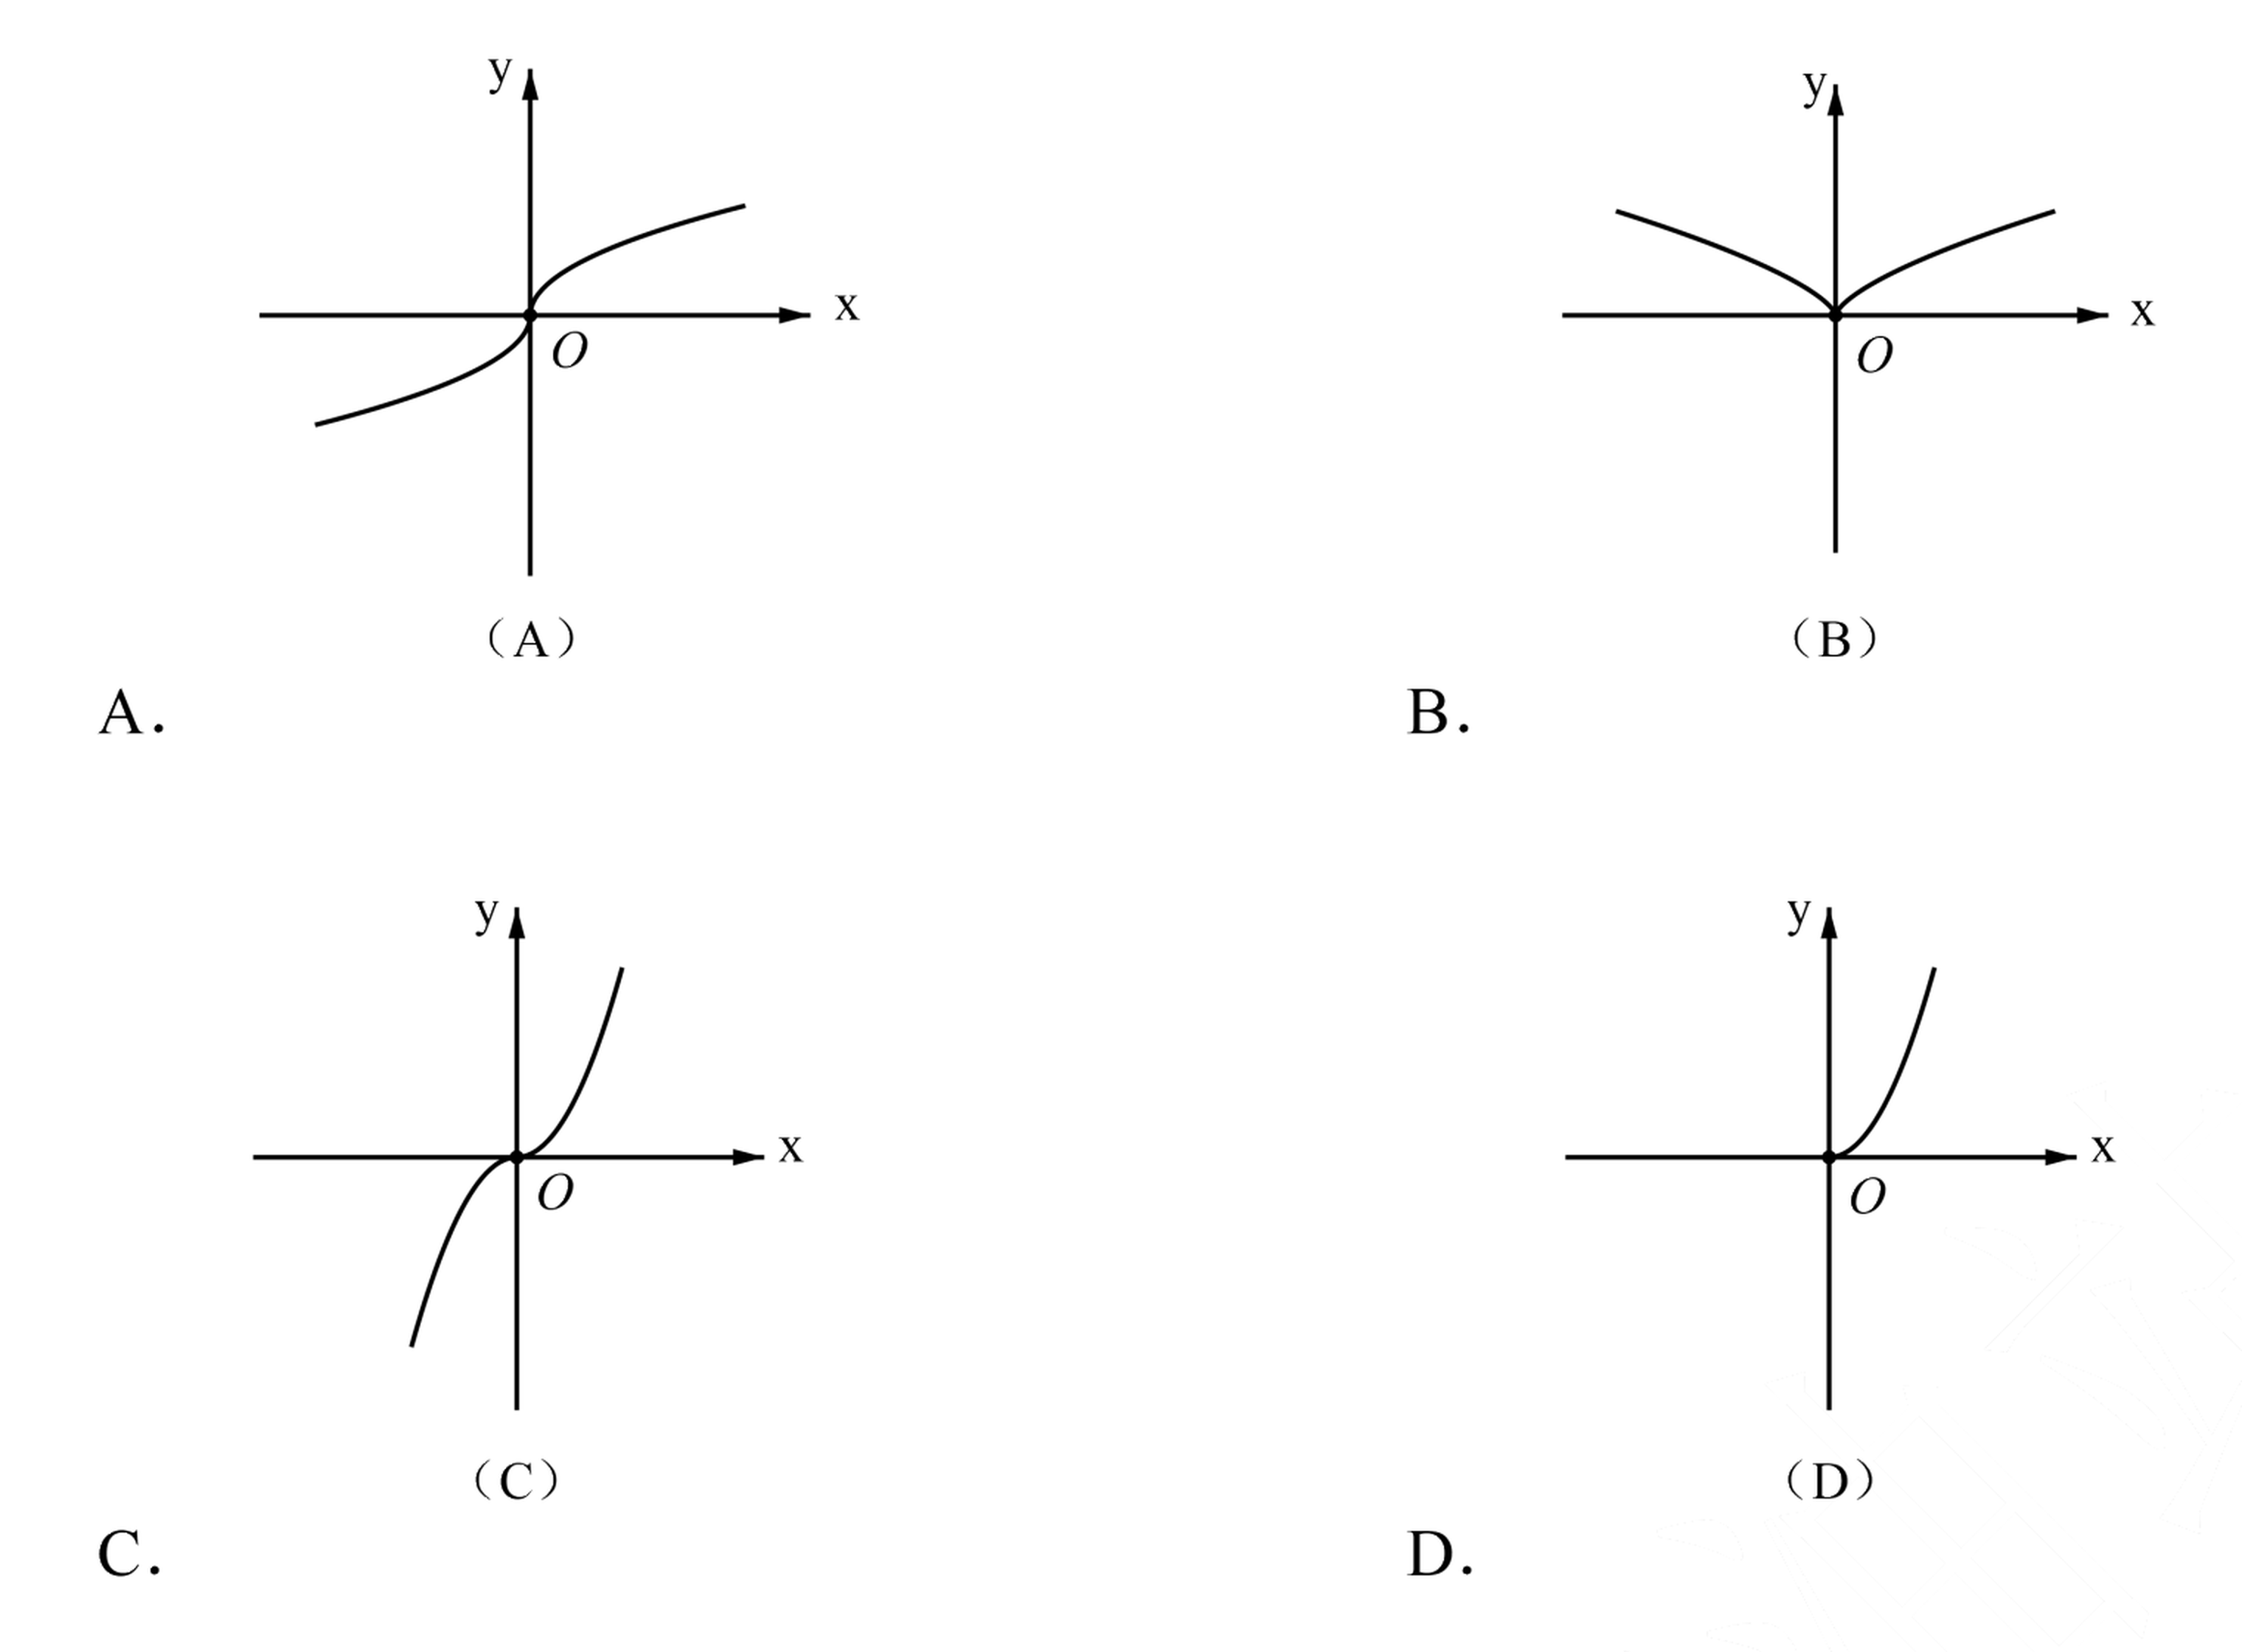
\includegraphics[width=0.80\textwidth]{figures/gao140_q14.png}
\end{center}

\ifanswer
\solbegin
\step{$f(x)=x^{\frac23}=\sqrt[3]{x^2}$ 是偶函数，且恒大于等于 $0$，故选 $B$.}
\solend
\fi

\item 设 $p$：关于 $x$ 的不等式 $x^2+ax+1>0$ 对 $x\in\R$ 恒成立，$q$：对数函数 $y=\log_{4-3a}x$ 在 $(0,+\infty)$ 上单调递减，那么 $p$ 是 $q$ 的\mbox{（\quad）}

\keepwithprev
A. 充分不必要条件\qquad B. 充要条件

C. 必要不充分条件\qquad D. 既不充分也不必要条件

\ifanswer
\solbegin
\step{$p\Leftrightarrow a^2-4<0\Leftrightarrow -2<a<2$. $q\Leftrightarrow 0<4-3a<1\Leftrightarrow 1<a<\dfrac43$.}
\step{由 $\left(1,\dfrac43\right)\subset(-2,2)$ 得 $q\Rightarrow p$；而 $a=0$ 时 $p$ 真、$q$ 假，}% 子集符号原卷印单线 $\subset$，照录
\step{故 $p$ 是 $q$ 的必要不充分条件，故选 $C$.}
\solend
\fi

\item “非空集合 $M$ 的元素都是集合 $P$ 的元素” 是假命题，现有下列命题：

(1) $M$ 的元素都不是 $P$ 的元素；(2) $M$ 中有不属于 $P$ 元素；% 原卷"不属于 P 元素"脱"的"字，照录

(3) $M$ 中有 $P$ 的元素；(4) $M$ 的元素不都是 $P$ 的元素，

其中真命题的个数是\mbox{（\quad）}

\keepwithprev
A. 1\qquad B. 2\qquad C. 3\qquad D. 4

\ifanswer
\solbegin
\step{由于 “非空集合 $M$ 的元素都是集合 $P$ 的元素” 是假命题，}
\step{得 “非空集合 $M$ 的元素至少有一个元素不属于集合 $P$” 是真命题.}
\step{则 (1) 不正确；(2) 正确；(3) $M$ 中不一定有 $P$ 的元素，例如 $M=\{a\}$，}
\step{则 $a\notin P$；(4) 正确.}
\step{综上，真命题只有 (2)(4). 故选 $B$.}
\solend
\fi

\end{enumerate}

\bigsec{三、解答题}

\begin{enumerate}
\setcounter{enumi}{16}

\item 设全集为 $\R$，集合 $A=\left\{x\mid\dfrac{2x}{x-1}\leqslant1\right\}$.

(1) 用区间表示集合 $A$；

(2) 若集合 $B=\{x\mid\lvert x+2\rvert+\lvert x-1\rvert=3\}$，求 $A\cup B$.

\ifanswer
\solbegin
\step{(1) 由 $\dfrac{2x}{x-1}\leqslant1\Leftrightarrow\dfrac{x+1}{x-1}\leqslant0$，故 $A=[-1,1)$，则 $\overline{A}=(-\infty,-1)\cup[1,+\infty)$；}
\step{(2) 由 $B=\{x\mid\lvert x+2\rvert+\lvert x-1\rvert=3\}=[-2,1]$，}
\step{结合上一问有 $A=[-1,1)$，所以 $A\cup B=B=[-2,1]$.}
\solend
\fi

\item (1) 已知指数函数 $y=a^x(a>0$ 且 $a\neq1)$ 在区间 $[-1,1]$ 上的最大值与最小值之和等于 $\dfrac52$，求实数 $a$ 的值.

(2) 已知幂函数 $y=x^{m^2+7m+10}(m\in\Z)$ 的图像关于 $y$ 轴对称，且在 $(0,+\infty)$ 上严格减. 若 $(a-1)^{m^2+7m+10}\geqslant(1+2a)^{m^2+7m+10}$. 求实数 $a$ 的取值范围.

\ifanswer
\solbegin
\step{(1) 指数函数 $y=a^x$ 在区间 $[-1,1]$ 上单调，所以 $a^1+a^{-1}=\dfrac52$，}
\step{所以 $a=2$ 或 $a=\dfrac12$；}
\step{(2) 由题意得 $m^2+7m+10<0$，所以 $-5<m<-2$，又因为 $m\in\Z$，}
\step{所以 $m=-4$ 或 $m=-3$，}
\step{当 $m=-4$ 时，$y=x^{m^2+7m+10}=x^{-2}$，为偶函数，}
\step{当 $m=-3$ 时，$y=x^{m^2+7m+10}=x^{-2}$，为偶函数，}
\step{所以 $m^2+7m+10=-2$，所以 $(a-1)^{-2}\geqslant(1+2a)^{-2}$，}
\step{所以 $\lvert a-1\rvert\leqslant\lvert 1+2a\rvert$，所以 $a\leqslant-2$ 或 $a\geqslant0$，所以 $a\in(-\infty,-2]\cup[0,+\infty)$.}
\solend
\fi

\item 设函数 $f(x)=ax^2+(1-a)x+a-2$ （$a\in\R$）.

(1) 若关于 $x$ 的不等式 $f(x)\leqslant0$ 的解集为 $\left[0,\dfrac12\right]$，求实数 $a$ 的值；

(2) 若 $a\geqslant0$，解关于 $x$ 的不等式：$f(x)<a-1$.

\ifanswer
\solbegin
\step{(1) 由解集得 $a>0$，且 $0$ 是方程 $f(x)=0$ 的根，故 $f(0)=a-2=0$，}
\step{得 $a=2$.}
\step{此时 $f(x)=2x^2-x=x(2x-1)$，$f(x)\leqslant0$ 的解集确为 $\left[0,\dfrac12\right]$.}
\step{(2) $f(x)<a-1\Leftrightarrow ax^2+(1-a)x-1<0\Leftrightarrow(x-1)(ax+1)<0$，}
\step{当 $a=0$ 时，$x-1<0$，解集为 $(-\infty,1)$.}
\step{当 $a>0$ 时，$-\dfrac1a<1$，解集为 $\left(-\dfrac1a,1\right)$.}
\solend
\fi

\item 为了保护环境，某单位采用新工艺，把二氧化碳转化为一种可利用的化工产品，已知该单位每月处理量最多不超过 $300$ 吨. 当月处理量为 $x$ 吨时，月处理成本为 $x^2-200x+40000(0<x\leqslant300)$ 元，且每处理一吨二氧化碳得到可利用的化工产品价值为 $300$ 元.

(1) 若要保证该单位每月不亏损，则每月处理量应控制在什么范围？

(2) 该单位每月处理量为多少吨时，才能使每吨的平均处理成本最低，最低为多少元？

\ifanswer
\solbegin
\step{(1) 由题意得 $S=300x-(x^2-200x+40000)$}
\step{$=-x^2+500x-40000(0<x\leqslant300)$，}
\step{令 $S\geqslant0$，即 $-x^2+500x-40000\geqslant0$，解得 $100\leqslant x\leqslant400$，}
\step{又 $0<x\leqslant300$，所以 $100\leqslant x\leqslant300$，}
\step{故要保证该单位每月不亏损，则每月处理量应控制在 $[100,300]$ 范围内；}
\step{(2) 每吨的平均出来成本为 $\dfrac yx=x+\dfrac{40000}x-200\geqslant2\sqrt{x\cdot\dfrac{40000}x}-200=200$，}% 原卷"平均出来成本"与题干"平均处理成本"措辞不一，照录
\step{当且仅当 $x=\dfrac{40000}x$，即 $x=200$ 时取等号，}
\step{所以该单位每月处理量为 $200$ 吨时，}
\step{才能使每吨的平均处理成本最低且最低为 $200$ 元.}
\solend
\fi

\item 已知函数 $y=f(x),x\in D$，若对于定义域 $D$ 内任意实数 $x,y$，不等式 $f(x)+f(y)\geqslant f(xy)$ 都成立，则称函数 $y=f(x)$ 是 $QB$ 函数，

(1) 判断函数 $f(x)=x+1$ 是否是 $QB$ 函数，并说明理由；

(2) 若函数 $g(x)=\ln(ax),x>0$ 是 $QB$ 函数，求实数 $a$ 的取值范围；

(3) 已知函数 $h(x)=a^x(a\in\R\text{ 且 }a>0)$，证明：“函数 $y=h(x)$ 是 $QB$ 函数” 的充要条件是 “ $a\in\{1\}$ ”.

\ifanswer
\solbegin
\step{(1) 不是，理由如下：因为 $f(x)=x+1$，}
\step{所以 $f(x)+f(y)\geqslant f(xy)\Leftrightarrow x+y\geqslant xy-1\Leftrightarrow(x-1)(y-1)\leqslant2$，}
\step{显然不恒成立，故不是 $QB$ 函数；}
\step{(2) 因为函数 $g(x)=\ln(ax),x>0$，则 $a>0$，}
\step{若函数 $g(x)$ 是 $QB$ 函数，则 $g(x)+g(y)\geqslant g(xy)$，}
\step{即 $\ln(ax)+\ln(ay)\geqslant\ln(axy)$，则 $\ln(a^2xy)\geqslant\ln(axy)$，得 $a^2xy\geqslant axy$，}
\step{且 $x>0,y>0$，得 $a^2\geqslant a$，解得 $a\geqslant1$ 或 $a\leqslant0$（舍去），}
\step{所以实数 $a$ 的取值范围为 $[1,+\infty)$.}
\step{(3) 若函数 $h(x)=a^x$ 是 $QB$ 函数，}
\step{当 $a>1$ 时，令 $x=y=\log_a\dfrac12$，则 $h(x)+h(y)=a^x+a^y=\dfrac12+\dfrac12=1$，}
\step{且 $h(xy)=a^{xy}=(a^x)^y=\left(\dfrac12\right)^{\log_a\frac12}=2^{\log_a2}$，}
\step{因为 $\log_a2>0$，所以 $h(xy)=2^{\log_a2}>1$，不满足 $h(x)+h(y)\geqslant h(xy)$，}
\step{不合题意；}
\step{当 $a=1$ 时，$h(x)+h(y)=a^x+a^y=1+1=2$，且 $h(xy)=a^{xy}=1$，}
\step{满足 $h(x)+h(y)\geqslant h(xy)$，符合题意；}
\step{当 $0<a<1$ 时，令 $x=\log_a2,y=2$，则 $h(x)+h(y)=a^x+a^y=2+a^2$，}
\step{且 $h(xy)=a^{xy}=(a^x)^y=2^2=4$，}
\step{因为 $0<a<1$，所以 $0<a^2<1$，得 $2<2+a^2<3$，}
\step{不满足 $h(x)+h(y)\geqslant h(xy)$，不合题意；}
\step{综上所述，$a\in\{1\}$，即充分性成立；}% 原卷"充分性/必要性"两标签与所证方向互换，照录
\step{若 $a\in\{1\}$，则 $h(x)+h(y)=a^x+a^y=1+1=2$，且 $h(xy)=a^{xy}=1$，}
\step{得 $h(x)+h(y)\geqslant h(xy)$，所以函数 $h(x)=a^x$ 是 $QB$ 函数，即必要性成立；}% 原卷"充分性/必要性"两标签与所证方向互换，照录
\step{综上所述，“函数 $y=h(x)$ 是 $QB$ 函数” 的充要条件是 “ $a\in\{1\}$ ”.}
\solend
\fi

\end{enumerate}

\end{document}
"
% 紧凑版：xelatex "\def\iscompact{1}% 高一140_甘泉外国语_期中.tex
%   —— 高一上数学"2026-2027 年甘泉外国语高一上期中"（试卷版/答案版）
% 试卷版：xelatex 高一140_甘泉外国语_期中.tex
% 答案版：xelatex "\def\isanswer{1}\input{高一140_甘泉外国语_期中.tex}"
% 紧凑版：xelatex "\def\iscompact{1}\input{高一140_甘泉外国语_期中.tex}"
%
% ① 原始材料：微信公众号"魔都数学加油站"文章，连载"27学年高一140"，原文标题
% "27学年高一140——2026-2027年上海市甘泉外国语高一上期中"；
% 原文链接：https://mp.weixin.qq.com/s/eflgf2Ktk1LyT9x-k-ltLw。
% 正文为 9 张 PNG 页（01、02、03、05、06、07、08 为 4762x6735；04、09 为 2560x3620，
% 同一篇各页分辨率不同，逐页按各自分辨率裁图核对），题目下印有【答案】或【解析】，为讲评版。
% 题目、解析均据原图转录；卷面粉红色水印"魔都数学加油站"及公众号页脚未录入。
% 全卷 1 幅插图：第 14 题四幅坐标函数图象选项（04 页），取原卷截图去粉色水印、去色、
% LANCZOS 放大 2 倍，四幅选项按原卷 2x2 排布（含（A）（B）（C）（D）图注与 A./B./C./D.
% 选项字母）合并裁为一张；图前按惯例加 \needvspace 守卫。
%
% 卷首标题：原卷印作"2026-2027 年甘泉外国语高一上期中"（公众号标题中的"上海市"
% 卷面标题行没有，本稿照卷面），年份区间按全稿惯例排 en dash；原卷未印副标题，
% 本卷为期中卷、跨集合与常用逻辑用语／不等式／函数三章，按题目内容标为
% "集合与常用逻辑用语、不等式、函数"（与 125／126／128／129／131／132／133 同期中卷口径相同）：
% 集合与逻辑见 Q5、Q13、Q15、Q16、Q17，不等式见 Q3、Q10、Q11、Q19、Q20，
% 函数（指数／对数／幂函数及其图象、同构与 QB 函数）见 Q4、Q6、Q7、Q8、Q12、Q14、Q18、Q21。
%
% 题号体例：本卷共 19 题——一、填空题 3—12（10 题）、二、选择题 13—16（4 题）、
% 三、解答题 17—21（5 题）。三节分别 \setcounter{enumi}{2}／{12}／{16}。
% 原卷从第 3 题起、无第 1、2 题，本稿保留原题号。
%
% ② 与原卷的排版差异：
%   ① 原文从第 3 题起，本稿保留原题号；
%   ② 原卷每题下直接印【答案】或【解析】，本稿按全稿惯例置于答案版；第 5 题只印
%      【答案】、无【解析】，提 \ans{}；第 13、14、15、16 题答案均在【解析】末句
%      "故选 …"，题干括号内留空、不另提 \ans{}；其余各题印【解析】、无独立答案段；
%      全卷无"答案印在题干括号内且无解析"的一型；
%   ③ 原卷未印副标题，本稿按"知识模块"口径补出；
%   ④ 原卷填空横线按全稿惯例排为 \blankline[4.4em]；选择题括号排 \mbox{（\quad）}、
%      每个选项段前按惯例加 \keepwithprev（四幅图选项那一枚放在 \begin{center} 之前）；
%      解答题不留作答区、不加 \anspace（原卷为讲评版，与 129／131／132／133／136 同）；
%   ⑤ 原卷数集混排：斜体 $R$（Q9、Q12、Q15 等）与黑体／黑板粗体 $R$（Q15、Q17、
%      Q19、Q21）、粗体 $Z$（Q18），按全稿惯例统一改 \R／\Z；空集记号 \varnothing；
%      绝对值排 \lvert…\rvert，集合描述竖线排 \mid；不等号按全稿惯例排 \leqslant／\geqslant；
%      补集照原卷上划线排 \overline{A}；
%   ⑥ 子题标号 (1)(2)(3)(4) 原卷印半角括号，照录（与 131／132／133／134／136 同口径）；
%      括注原卷全角／半角混用，逐处照录：Q8"（结果用 a,b 表示）"、Q19"（a∈R）"、
%      Q21 (2)"（舍去）"印全角，Q18"$a^x(a>0$ 且 $a\neq1)$"、Q20"$40000(0<x\leqslant300)$"、
%      Q21 (3)"($a\in\R$ 且 $a>0$)"及 (0,+∞)、2(a>0) 等数学式内括注印半角；
%   ⑦ 数学式内半角逗号照录（如 Q8"$\lg2=a,10^b=3$"、Q11"$-2,3,4,\cdots,2027$"、
%      Q12"$x_1,x_2$"、Q19"$f(x)=ax^2+(1-a)x+a-2$"、Q21"$x>0,y>0$"）；
%      原卷行末西文句点照录（Q20 题干"300 吨. 当月处理量为 x 吨时"），行中全角逗号照录；
%   ⑧ 一幅插图：第 14 题四幅坐标函数图象选项合并裁为一张 \includegraphics
%      （题前 \needvspace{9cm}）。Q14 是"二、选择题"节内带大图块的第二题
%      （Q13 为节首题但无图），另在 \bigsec{二、选择题} 之前加 \needvspace{11cm}
%      连节标题一起量——守卫必须放在 \bigsec 之前，放标题之后会让"二、选择题"
%      孤立在页末（B 类，照 高一26／40／59／136 成例）；三版切页审计均"合计异常：无"；
%   ⑨ 跨页续印按题合并：Q9 题干在 01 页、解析续至 02 页；Q11 题干与解析前 3 行在 02 页、
%      后 2 行在 03 页；Q14 题干在 03 页末、四幅图与【解析】在 04 页；Q16 题干四条命题
%      在 04 页、选项与【解析】在 05 页；Q18 解析 (1) 首行在 05 页、其余 7 行在 06 页；
%      Q20 题干在 06 页末、"300 元."与两小问及【解析】在 07 页；Q21 解析跨 07—09 页
%      （末 3 行在 09 页）；本稿按题连排，不丢行；
%   ⑩ 题干中的中文弯引号按原卷照录，注释内一律 ASCII 引号；原卷"图像／图象"
%      两种写法混用，逐处照录（Q7、Q18 作"图像"，Q14 作"图象"）；
%   ⑪ 原卷无红色加粗标签（【解析】【答案】均黑色印刷），故本卷未用 \stepm。
%
% 判别式字形：全卷仅第 9 题【解析】"经验证得"cases 块出现两处判别式
%   "$\Delta=p^2-4q>0$"与"$\Delta'=q^2-4p>0$"，原卷两处均印等腰、偏高的
%   三角 $\Delta$（带撇的为 $\Delta'$），逐处放大核对并照录 \Delta、\Delta'；
%   全卷未出现扁等边三角 \triangle。
%
% 子集符号：第 15 题【解析】"由 (1,4/3)⊂(-2,2) 得 q⇒p"一处原卷印单线 $\subset$
%   （不带下划线），逐处放大核对、照录 \subset；全卷未出现带下划线的 \subseteq。
%
% 原卷存疑照录（均照录未改，正文对应处另有 % 注）：
%   第 16 题 (2) 命题"$M$ 中有不属于 $P$ 元素"中"不属于 $P$ 元素"脱"的"字，照录；
%   第 20 题题干 (2) 作"每吨的平均处理成本"、而【解析】(2) 作"每吨的平均出来成本"，
%      "出来"疑为"处理"之误，两处措辞照录不统一；
%   第 21 题 (3)【解析】"综上所述，$a\in\{1\}$，即充分性成立"与"即必要性成立"
%      两处标签与所证方向互换（按充要条件的通常口径），照录。
%
% 行数复核：一条 \step = 原卷解析的一个印刷行，cases 块作一个印刷行计。逐题数 \step
%   条数，合计 92 条（Q3：2；Q4：1；Q5：0；Q6：2；Q7：1；Q8：1；Q9：7；Q10：5；
%   Q11：5；Q12：4；Q13：6；Q14：1；Q15：3；Q16：5；Q17：3；Q18：8；Q19：6；
%   Q20：9；Q21：23），与原卷印刷行逐题相等。第 5 题只印【答案】、提 \ans{}，
%   不计入 \step 账；第 13、14、15、16 题答案在解析末句"故选 …"，括号内留空、
%   不另提 \ans{}；答案版【答案】/【解析】标记数 = 19（1 个 \ans + 18 个 \solbegin）
%   = 全卷题数。
%
\documentclass[a4paper,11pt]{article}
\usepackage{common}

\begin{document}

\examtitlest[3]{2026--2027 年甘泉外国语高一上期中}{集合与常用逻辑用语、不等式、函数}

\bigsec{一、填空题}

\begin{enumerate}
\setcounter{enumi}{2}

\item 不等式 $x^2-2x-3<0$ 的解集为\blankline[4.4em].

\ifanswer
\solbegin
\step{方程 $x^2-2x-3=0$ 的实数根是 $x_1=-1$，$x_2=3$；}
\step{所以不等式 $x^2-2x-3<0$ 的解集为 $\{x\mid -1<x<3\}$.}
\solend
\fi

\item 根式 $\sqrt{x\sqrt{x}}(x>0)$ 的指数幂形式为\blankline[4.4em].

\ifanswer
\solbegin
\step{$\sqrt{x\sqrt{x}}=\sqrt{x\cdot x^{\frac12}}=\sqrt{x^{\frac32}}=x^{\frac34}$.}
\solend
\fi

\item 陈述句 “ $x>1$ 或 $y>1$ ” 的否定形式是\blankline[4.4em].

\ifanswer
\ans{$x\leqslant1$ 且 $y\leqslant1$}
\fi

\item 若 $x<0$ 时，指数函数 $y=(a-1)^x$ 的值总大于 $1$，则实数 $a$ 的取值范围是\blankline[4.4em].

\ifanswer
\solbegin
\step{由题意得 $(a-1)^x>1$ 在 $(-\infty,0)$ 上恒成立，则 $0<a-1<1$，解得 $1<a<2$.}
\step{故实数 $a$ 的取值范围是 $(1,2)$.}
\solend
\fi

\item 若 $f(x)=\log_a(x-1)$，对任意 $a>0$ 且 $a\neq1$，函数 $y=f(x)$ 的图像必过定点\blankline[4.4em].

\ifanswer
\solbegin
\step{令 $x-1=1$，即 $x=2$，此时 $f(2)=0$，即函数图像过定点 $(2,0)$.}
\solend
\fi

\item 已知 $\lg 2=a,10^b=3$，则 $\log_6 2=$\blankline[4.4em]（结果用 $a,b$ 表示）.

\ifanswer
\solbegin
\step{由 $10^b=3$，得 $b=\lg 3$，则 $\log_6 2=\dfrac{\lg 2}{\lg 6}=\dfrac{\lg 2}{\lg 2+\lg 3}=\dfrac{a}{a+b}$.}
\solend
\fi

\item 已知 $p$、$q\in\R$，$x_1$、$x_2$ 是关于 $x$ 的方程 $x^2+px+q=0$ 的两实根，$x_1+1$、$x_2+1$ 是关于 $x$ 的方程 $x^2+qx+p=0$ 的两实根，则 $pq=$\blankline[4.4em].

\ifanswer
\solbegin
\step{因为 $x_1$、$x_2$ 是关于 $x$ 的方程 $x^2+px+q=0$ 的两实根，}
\step{由韦达定理得 $x_1+x_2=-p$，$x_1\cdot x_2=q$，}
\step{因为 $x_1+1$、$x_2+1$ 是关于 $x$ 的方程 $x^2+qx+p=0$ 的两实根，}
\step{由韦达定理得 $x_1+1+x_2+1=-q$，$(x_1+1)(x_2+1)=p$，}
\step{即 $x_1+x_2=-q-2$，$x_1+x_2+x_1x_2=p-1$，又 $x_1+x_2=-p$，$x_1\cdot x_2=q$，}
\step{所以 $\begin{cases}-p=-q-2\\-p+q=p-1\end{cases}$，解得 $\begin{cases}p=-1\\q=-3\end{cases}$，经验证得 $\begin{cases}\Delta=p^2-4q>0\\\Delta'=q^2-4p>0\end{cases}$，}% 判别式原卷印高三角 $\Delta$、$\Delta'$，照录
\step{则 $pq=3$.}
\solend
\fi

\item 对于 $x\in\R$，不等式 $\lvert 3-x\rvert+\lvert 1+x\rvert\geqslant a^2-3a$ 恒成立，则实数 $a$ 的取值范围是\blankline[4.4em].

\ifanswer
\solbegin
\step{对于 $x\in\R$，不等式 $\lvert 3-x\rvert+\lvert 1+x\rvert\geqslant a^2-3a$ 恒成立，}
\step{即 $\lvert 3-x\rvert+\lvert 1+x\rvert$ 的最小值大于或等于 $a^2-3a$，}
\step{$\lvert 3-x\rvert+\lvert 1+x\rvert$ 表示数轴上的 $x$ 对应点到 $3$ 和 $-1$ 对应点的距离之和，}
\step{它的最小值为 $4$，故 $4\geqslant a^2-3a$，即 $a^2-3a-4\leqslant0$，解得 $-1\leqslant a\leqslant4$，}
\step{故实数 $a$ 的取值范围是 $[-1,4]$.}
\solend
\fi

\item 已知同时满足不等式 $x^2-x-2>0$ 和 $2x^2+(5+2a)x+5a<0$ 的 $x$ 的整数值只有 $2026$ 个，则实数 $a$ 的取值范围是\blankline[4.4em].

\ifanswer
\solbegin
\step{整数 $x$ 须满足 $x\leqslant-2$ 或 $x\geqslant3$，且 $(2x+5)(x+a)<0$.}
\step{当 $a<\dfrac52$ 时，需使整数解恰为 $-2,3,4,\cdots,2027$，即 $2027<-a\leqslant2028$.}
\step{当 $a>\dfrac52$ 时，需使整数解恰为 $-2028,-2027,\cdots,-3$，即 $2028<a\leqslant2029$；}
\step{$a=\dfrac52$ 时无解.}
\step{故 $a\in[-2028,-2027)\cup(2028,2029]$.}
\solend
\fi

\item 同构式通俗讲是结构相同的表达式，如：$f(x)=x+e^x$，$f(\ln x)=\ln x+e^{\ln x}=\ln x+x$，称 $x+e^x$ 与 $\ln x+x$ 为同构式. 已知实数 $x_1,x_2$ 满足 $e^{x_1}+x_1=8,\ln\sqrt[5]{5x_2+3}+x_2=1$，则 $x_1+5x_2=$\blankline[4.4em].

\ifanswer
\solbegin
\step{函数 $f(x)=x+e^x$ 在 $\R$ 上严格增，且 $f(x_1)=x_1+e^{x_1}=8$，}
\step{由 $\ln\sqrt[5]{5x_2+3}+x_2=1$，得 $\ln(5x_2+3)+5x_2=5$，则 $\ln(5x_2+3)+5x_2+3=8$，}
\step{即 $f(\ln(5x_2+3))=8$，因此 $f(\ln(5x_2+3))=8=f(x_1)$，则 $x_1=\ln(5x_2+3)$，}
\step{所以 $x_1+5x_2=\ln(5x_2+3)+5x_2=5$.}
\solend
\fi

\end{enumerate}

% 第 14 题四幅图是"二、选择题"节内的大图块；守卫须放在 \bigsec 之前连节标题一起量，
% 否则"二、选择题"会孤立在页末（B 类，照 高一26／40／59／136 成例）
\needvspace{11cm}
\bigsec{二、选择题}

\begin{enumerate}
\setcounter{enumi}{12}

\item 设 $a$、$b$ 为实数，则 “ $a>b>0$ ” 的一个充分非必要条件是\mbox{（\quad）}

\keepwithprev
A. $\sqrt{a-1}>\sqrt{b-1}$\qquad B. $a^2>b^2$

C. $\dfrac1b>\dfrac1a$\qquad D. $a-b>b-a$

\ifanswer
\solbegin
\step{由 $\sqrt{a-1}>\sqrt{b-1}$ 得 $a>b\geqslant1$，故 $a>b>0$，反之不成立，满足题意；}
\step{由 $a^2>b^2$，则 $\lvert a\rvert>\lvert b\rvert$，推不出 $a>b>0$，反向可推出，不满足；}
\step{由 $\dfrac1b>\dfrac1a$，则 $a>b>0$ 或 $b>0>a$ 或 $0>a>b$，推不出 $a>b>0$，}
\step{反向可推出，不满足；}
\step{由 $a-b>b-a$，则 $a>b$，推不出 $a>b>0$，反向可推出，不满足；}
\step{故选 $A$.}
\solend
\fi

% 第 14 题四幅坐标函数图象选项是一整块，守卫放在 \item 之前
\needvspace{9cm}
\item 幂函数 $f(x)=x^{\frac23}$ 的图象大致为\mbox{（\quad）}

\keepwithprev
\begin{center}
% 四幅坐标函数图象选项取原卷 04 页截图去粉色水印、去色，按原卷 2x2 排布合并为一张
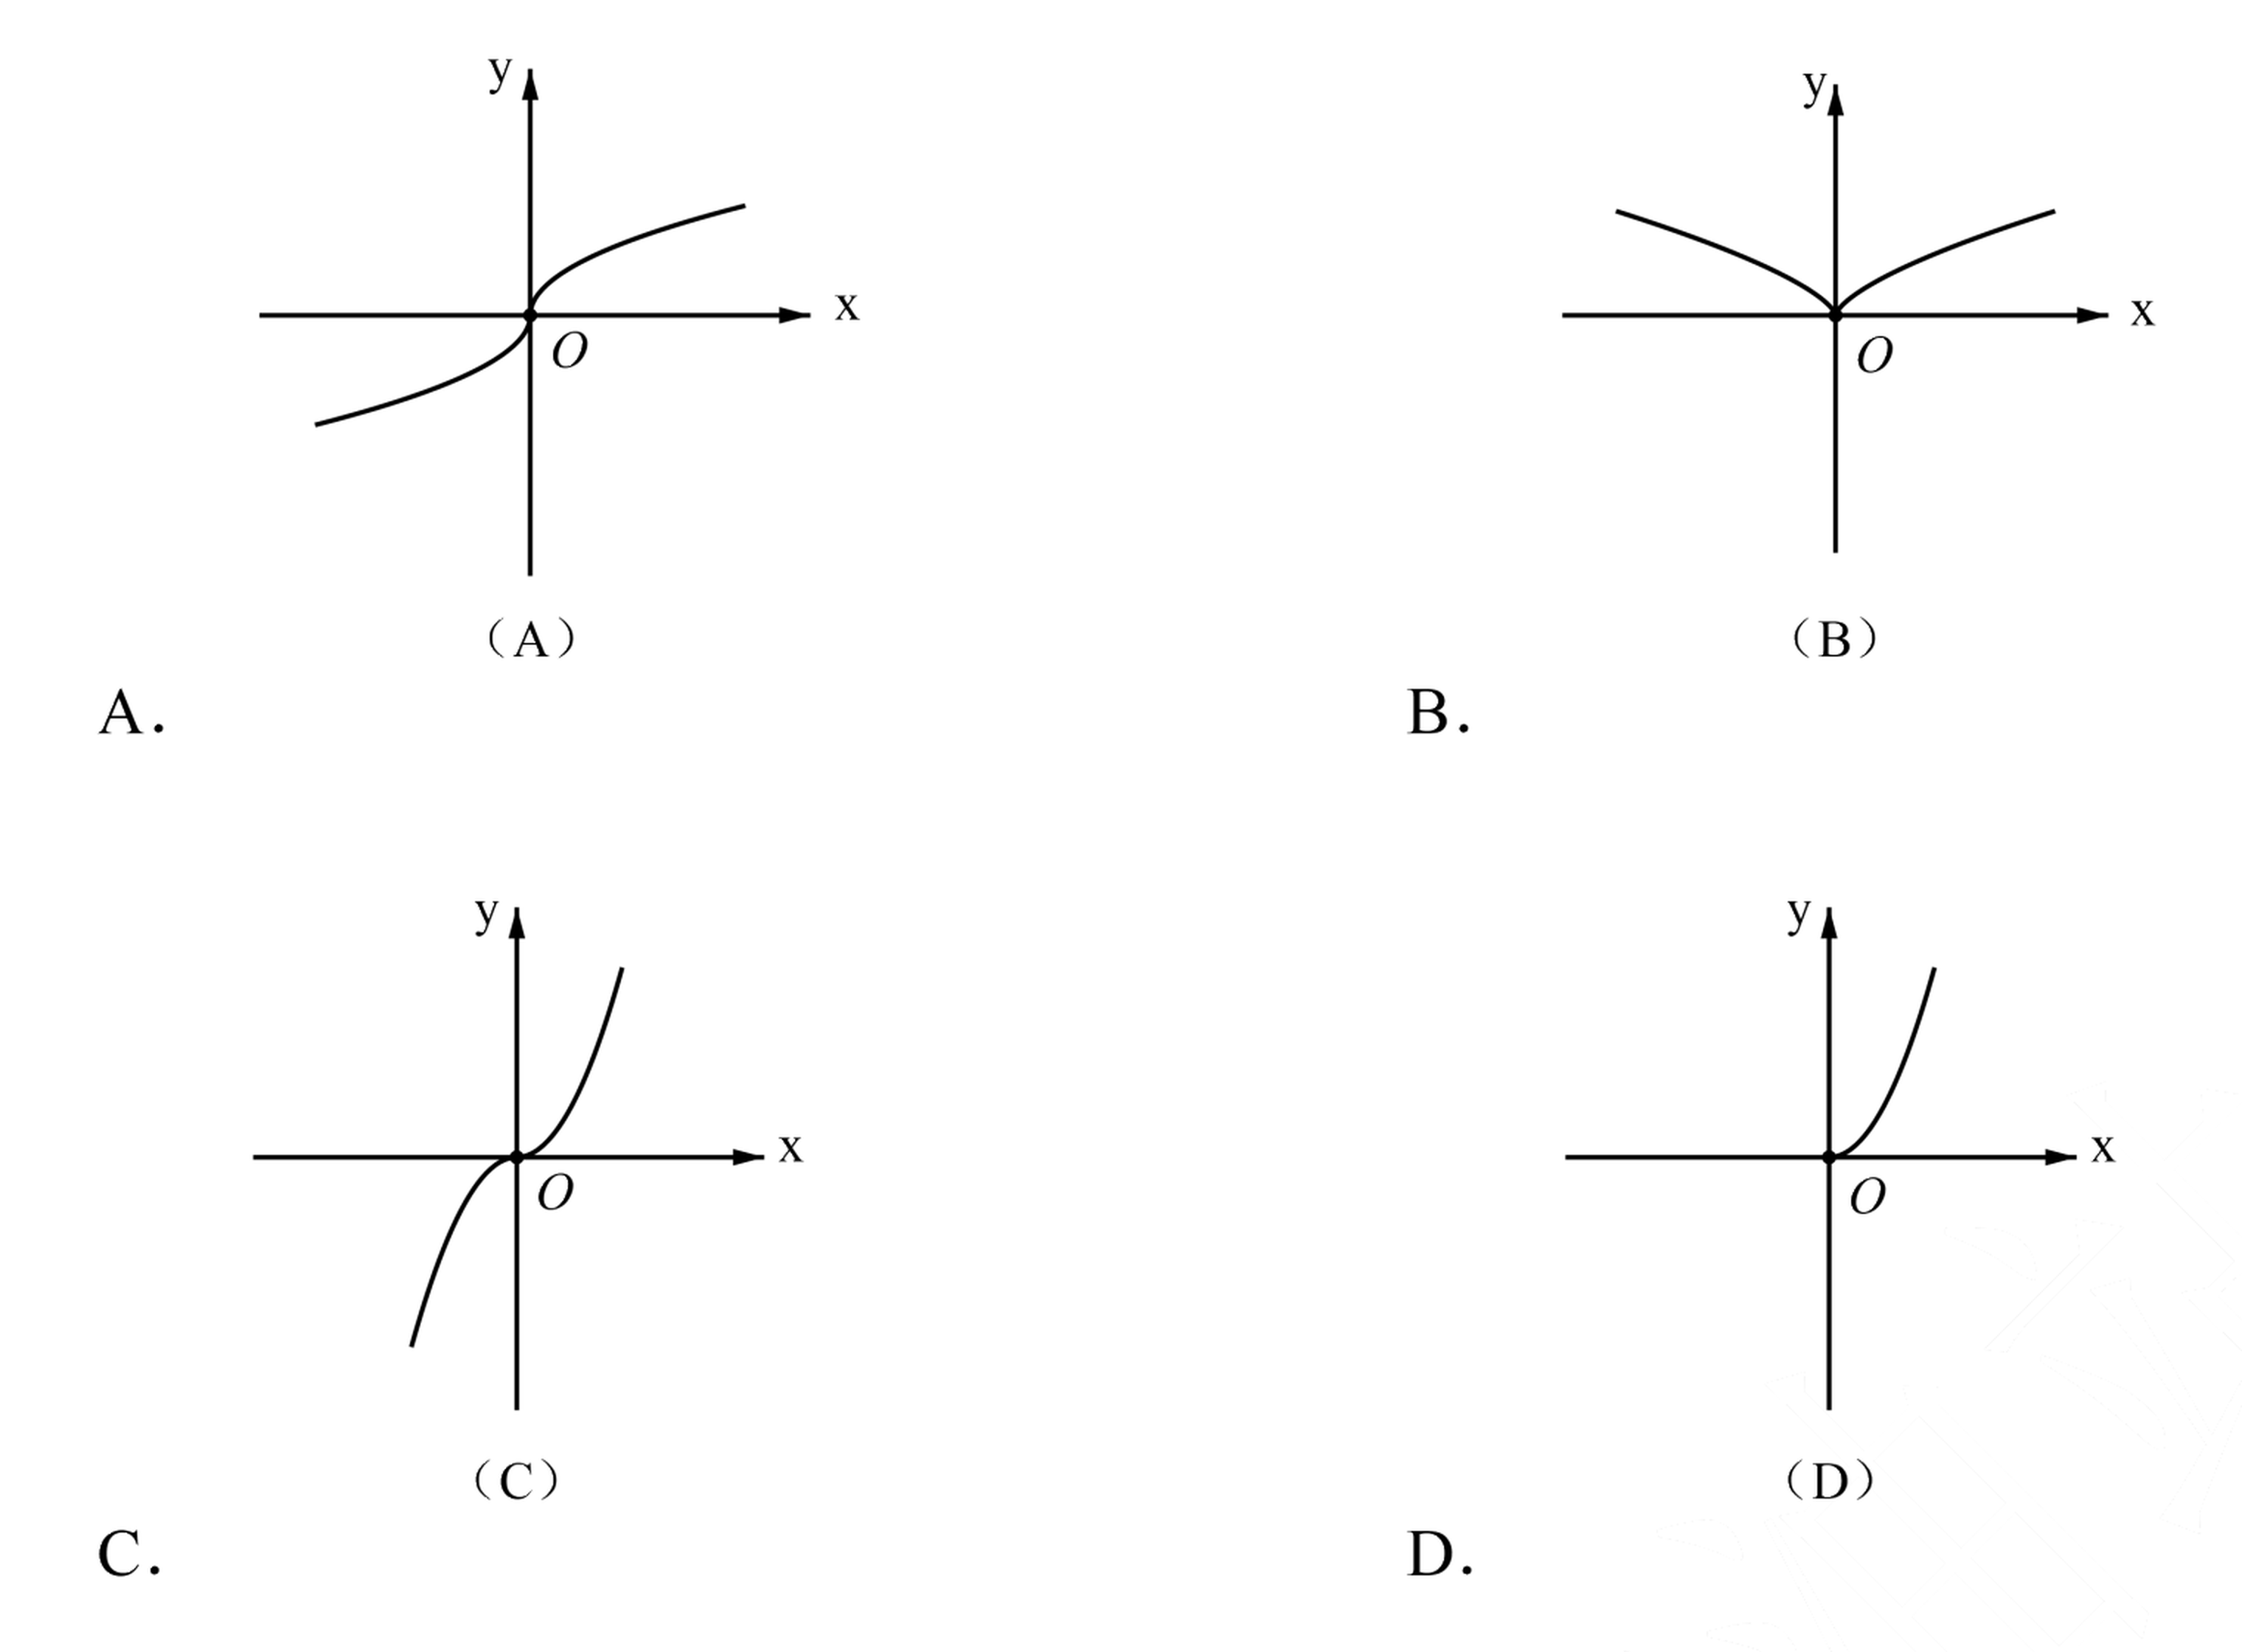
\includegraphics[width=0.80\textwidth]{figures/gao140_q14.png}
\end{center}

\ifanswer
\solbegin
\step{$f(x)=x^{\frac23}=\sqrt[3]{x^2}$ 是偶函数，且恒大于等于 $0$，故选 $B$.}
\solend
\fi

\item 设 $p$：关于 $x$ 的不等式 $x^2+ax+1>0$ 对 $x\in\R$ 恒成立，$q$：对数函数 $y=\log_{4-3a}x$ 在 $(0,+\infty)$ 上单调递减，那么 $p$ 是 $q$ 的\mbox{（\quad）}

\keepwithprev
A. 充分不必要条件\qquad B. 充要条件

C. 必要不充分条件\qquad D. 既不充分也不必要条件

\ifanswer
\solbegin
\step{$p\Leftrightarrow a^2-4<0\Leftrightarrow -2<a<2$. $q\Leftrightarrow 0<4-3a<1\Leftrightarrow 1<a<\dfrac43$.}
\step{由 $\left(1,\dfrac43\right)\subset(-2,2)$ 得 $q\Rightarrow p$；而 $a=0$ 时 $p$ 真、$q$ 假，}% 子集符号原卷印单线 $\subset$，照录
\step{故 $p$ 是 $q$ 的必要不充分条件，故选 $C$.}
\solend
\fi

\item “非空集合 $M$ 的元素都是集合 $P$ 的元素” 是假命题，现有下列命题：

(1) $M$ 的元素都不是 $P$ 的元素；(2) $M$ 中有不属于 $P$ 元素；% 原卷"不属于 P 元素"脱"的"字，照录

(3) $M$ 中有 $P$ 的元素；(4) $M$ 的元素不都是 $P$ 的元素，

其中真命题的个数是\mbox{（\quad）}

\keepwithprev
A. 1\qquad B. 2\qquad C. 3\qquad D. 4

\ifanswer
\solbegin
\step{由于 “非空集合 $M$ 的元素都是集合 $P$ 的元素” 是假命题，}
\step{得 “非空集合 $M$ 的元素至少有一个元素不属于集合 $P$” 是真命题.}
\step{则 (1) 不正确；(2) 正确；(3) $M$ 中不一定有 $P$ 的元素，例如 $M=\{a\}$，}
\step{则 $a\notin P$；(4) 正确.}
\step{综上，真命题只有 (2)(4). 故选 $B$.}
\solend
\fi

\end{enumerate}

\bigsec{三、解答题}

\begin{enumerate}
\setcounter{enumi}{16}

\item 设全集为 $\R$，集合 $A=\left\{x\mid\dfrac{2x}{x-1}\leqslant1\right\}$.

(1) 用区间表示集合 $A$；

(2) 若集合 $B=\{x\mid\lvert x+2\rvert+\lvert x-1\rvert=3\}$，求 $A\cup B$.

\ifanswer
\solbegin
\step{(1) 由 $\dfrac{2x}{x-1}\leqslant1\Leftrightarrow\dfrac{x+1}{x-1}\leqslant0$，故 $A=[-1,1)$，则 $\overline{A}=(-\infty,-1)\cup[1,+\infty)$；}
\step{(2) 由 $B=\{x\mid\lvert x+2\rvert+\lvert x-1\rvert=3\}=[-2,1]$，}
\step{结合上一问有 $A=[-1,1)$，所以 $A\cup B=B=[-2,1]$.}
\solend
\fi

\item (1) 已知指数函数 $y=a^x(a>0$ 且 $a\neq1)$ 在区间 $[-1,1]$ 上的最大值与最小值之和等于 $\dfrac52$，求实数 $a$ 的值.

(2) 已知幂函数 $y=x^{m^2+7m+10}(m\in\Z)$ 的图像关于 $y$ 轴对称，且在 $(0,+\infty)$ 上严格减. 若 $(a-1)^{m^2+7m+10}\geqslant(1+2a)^{m^2+7m+10}$. 求实数 $a$ 的取值范围.

\ifanswer
\solbegin
\step{(1) 指数函数 $y=a^x$ 在区间 $[-1,1]$ 上单调，所以 $a^1+a^{-1}=\dfrac52$，}
\step{所以 $a=2$ 或 $a=\dfrac12$；}
\step{(2) 由题意得 $m^2+7m+10<0$，所以 $-5<m<-2$，又因为 $m\in\Z$，}
\step{所以 $m=-4$ 或 $m=-3$，}
\step{当 $m=-4$ 时，$y=x^{m^2+7m+10}=x^{-2}$，为偶函数，}
\step{当 $m=-3$ 时，$y=x^{m^2+7m+10}=x^{-2}$，为偶函数，}
\step{所以 $m^2+7m+10=-2$，所以 $(a-1)^{-2}\geqslant(1+2a)^{-2}$，}
\step{所以 $\lvert a-1\rvert\leqslant\lvert 1+2a\rvert$，所以 $a\leqslant-2$ 或 $a\geqslant0$，所以 $a\in(-\infty,-2]\cup[0,+\infty)$.}
\solend
\fi

\item 设函数 $f(x)=ax^2+(1-a)x+a-2$ （$a\in\R$）.

(1) 若关于 $x$ 的不等式 $f(x)\leqslant0$ 的解集为 $\left[0,\dfrac12\right]$，求实数 $a$ 的值；

(2) 若 $a\geqslant0$，解关于 $x$ 的不等式：$f(x)<a-1$.

\ifanswer
\solbegin
\step{(1) 由解集得 $a>0$，且 $0$ 是方程 $f(x)=0$ 的根，故 $f(0)=a-2=0$，}
\step{得 $a=2$.}
\step{此时 $f(x)=2x^2-x=x(2x-1)$，$f(x)\leqslant0$ 的解集确为 $\left[0,\dfrac12\right]$.}
\step{(2) $f(x)<a-1\Leftrightarrow ax^2+(1-a)x-1<0\Leftrightarrow(x-1)(ax+1)<0$，}
\step{当 $a=0$ 时，$x-1<0$，解集为 $(-\infty,1)$.}
\step{当 $a>0$ 时，$-\dfrac1a<1$，解集为 $\left(-\dfrac1a,1\right)$.}
\solend
\fi

\item 为了保护环境，某单位采用新工艺，把二氧化碳转化为一种可利用的化工产品，已知该单位每月处理量最多不超过 $300$ 吨. 当月处理量为 $x$ 吨时，月处理成本为 $x^2-200x+40000(0<x\leqslant300)$ 元，且每处理一吨二氧化碳得到可利用的化工产品价值为 $300$ 元.

(1) 若要保证该单位每月不亏损，则每月处理量应控制在什么范围？

(2) 该单位每月处理量为多少吨时，才能使每吨的平均处理成本最低，最低为多少元？

\ifanswer
\solbegin
\step{(1) 由题意得 $S=300x-(x^2-200x+40000)$}
\step{$=-x^2+500x-40000(0<x\leqslant300)$，}
\step{令 $S\geqslant0$，即 $-x^2+500x-40000\geqslant0$，解得 $100\leqslant x\leqslant400$，}
\step{又 $0<x\leqslant300$，所以 $100\leqslant x\leqslant300$，}
\step{故要保证该单位每月不亏损，则每月处理量应控制在 $[100,300]$ 范围内；}
\step{(2) 每吨的平均出来成本为 $\dfrac yx=x+\dfrac{40000}x-200\geqslant2\sqrt{x\cdot\dfrac{40000}x}-200=200$，}% 原卷"平均出来成本"与题干"平均处理成本"措辞不一，照录
\step{当且仅当 $x=\dfrac{40000}x$，即 $x=200$ 时取等号，}
\step{所以该单位每月处理量为 $200$ 吨时，}
\step{才能使每吨的平均处理成本最低且最低为 $200$ 元.}
\solend
\fi

\item 已知函数 $y=f(x),x\in D$，若对于定义域 $D$ 内任意实数 $x,y$，不等式 $f(x)+f(y)\geqslant f(xy)$ 都成立，则称函数 $y=f(x)$ 是 $QB$ 函数，

(1) 判断函数 $f(x)=x+1$ 是否是 $QB$ 函数，并说明理由；

(2) 若函数 $g(x)=\ln(ax),x>0$ 是 $QB$ 函数，求实数 $a$ 的取值范围；

(3) 已知函数 $h(x)=a^x(a\in\R\text{ 且 }a>0)$，证明：“函数 $y=h(x)$ 是 $QB$ 函数” 的充要条件是 “ $a\in\{1\}$ ”.

\ifanswer
\solbegin
\step{(1) 不是，理由如下：因为 $f(x)=x+1$，}
\step{所以 $f(x)+f(y)\geqslant f(xy)\Leftrightarrow x+y\geqslant xy-1\Leftrightarrow(x-1)(y-1)\leqslant2$，}
\step{显然不恒成立，故不是 $QB$ 函数；}
\step{(2) 因为函数 $g(x)=\ln(ax),x>0$，则 $a>0$，}
\step{若函数 $g(x)$ 是 $QB$ 函数，则 $g(x)+g(y)\geqslant g(xy)$，}
\step{即 $\ln(ax)+\ln(ay)\geqslant\ln(axy)$，则 $\ln(a^2xy)\geqslant\ln(axy)$，得 $a^2xy\geqslant axy$，}
\step{且 $x>0,y>0$，得 $a^2\geqslant a$，解得 $a\geqslant1$ 或 $a\leqslant0$（舍去），}
\step{所以实数 $a$ 的取值范围为 $[1,+\infty)$.}
\step{(3) 若函数 $h(x)=a^x$ 是 $QB$ 函数，}
\step{当 $a>1$ 时，令 $x=y=\log_a\dfrac12$，则 $h(x)+h(y)=a^x+a^y=\dfrac12+\dfrac12=1$，}
\step{且 $h(xy)=a^{xy}=(a^x)^y=\left(\dfrac12\right)^{\log_a\frac12}=2^{\log_a2}$，}
\step{因为 $\log_a2>0$，所以 $h(xy)=2^{\log_a2}>1$，不满足 $h(x)+h(y)\geqslant h(xy)$，}
\step{不合题意；}
\step{当 $a=1$ 时，$h(x)+h(y)=a^x+a^y=1+1=2$，且 $h(xy)=a^{xy}=1$，}
\step{满足 $h(x)+h(y)\geqslant h(xy)$，符合题意；}
\step{当 $0<a<1$ 时，令 $x=\log_a2,y=2$，则 $h(x)+h(y)=a^x+a^y=2+a^2$，}
\step{且 $h(xy)=a^{xy}=(a^x)^y=2^2=4$，}
\step{因为 $0<a<1$，所以 $0<a^2<1$，得 $2<2+a^2<3$，}
\step{不满足 $h(x)+h(y)\geqslant h(xy)$，不合题意；}
\step{综上所述，$a\in\{1\}$，即充分性成立；}% 原卷"充分性/必要性"两标签与所证方向互换，照录
\step{若 $a\in\{1\}$，则 $h(x)+h(y)=a^x+a^y=1+1=2$，且 $h(xy)=a^{xy}=1$，}
\step{得 $h(x)+h(y)\geqslant h(xy)$，所以函数 $h(x)=a^x$ 是 $QB$ 函数，即必要性成立；}% 原卷"充分性/必要性"两标签与所证方向互换，照录
\step{综上所述，“函数 $y=h(x)$ 是 $QB$ 函数” 的充要条件是 “ $a\in\{1\}$ ”.}
\solend
\fi

\end{enumerate}

\end{document}
"
%
% ① 原始材料：微信公众号"魔都数学加油站"文章，连载"27学年高一140"，原文标题
% "27学年高一140——2026-2027年上海市甘泉外国语高一上期中"；
% 原文链接：https://mp.weixin.qq.com/s/eflgf2Ktk1LyT9x-k-ltLw。
% 正文为 9 张 PNG 页（01、02、03、05、06、07、08 为 4762x6735；04、09 为 2560x3620，
% 同一篇各页分辨率不同，逐页按各自分辨率裁图核对），题目下印有【答案】或【解析】，为讲评版。
% 题目、解析均据原图转录；卷面粉红色水印"魔都数学加油站"及公众号页脚未录入。
% 全卷 1 幅插图：第 14 题四幅坐标函数图象选项（04 页），取原卷截图去粉色水印、去色、
% LANCZOS 放大 2 倍，四幅选项按原卷 2x2 排布（含（A）（B）（C）（D）图注与 A./B./C./D.
% 选项字母）合并裁为一张；图前按惯例加 \needvspace 守卫。
%
% 卷首标题：原卷印作"2026-2027 年甘泉外国语高一上期中"（公众号标题中的"上海市"
% 卷面标题行没有，本稿照卷面），年份区间按全稿惯例排 en dash；原卷未印副标题，
% 本卷为期中卷、跨集合与常用逻辑用语／不等式／函数三章，按题目内容标为
% "集合与常用逻辑用语、不等式、函数"（与 125／126／128／129／131／132／133 同期中卷口径相同）：
% 集合与逻辑见 Q5、Q13、Q15、Q16、Q17，不等式见 Q3、Q10、Q11、Q19、Q20，
% 函数（指数／对数／幂函数及其图象、同构与 QB 函数）见 Q4、Q6、Q7、Q8、Q12、Q14、Q18、Q21。
%
% 题号体例：本卷共 19 题——一、填空题 3—12（10 题）、二、选择题 13—16（4 题）、
% 三、解答题 17—21（5 题）。三节分别 \setcounter{enumi}{2}／{12}／{16}。
% 原卷从第 3 题起、无第 1、2 题，本稿保留原题号。
%
% ② 与原卷的排版差异：
%   ① 原文从第 3 题起，本稿保留原题号；
%   ② 原卷每题下直接印【答案】或【解析】，本稿按全稿惯例置于答案版；第 5 题只印
%      【答案】、无【解析】，提 \ans{}；第 13、14、15、16 题答案均在【解析】末句
%      "故选 …"，题干括号内留空、不另提 \ans{}；其余各题印【解析】、无独立答案段；
%      全卷无"答案印在题干括号内且无解析"的一型；
%   ③ 原卷未印副标题，本稿按"知识模块"口径补出；
%   ④ 原卷填空横线按全稿惯例排为 \blankline[4.4em]；选择题括号排 \mbox{（\quad）}、
%      每个选项段前按惯例加 \keepwithprev（四幅图选项那一枚放在 \begin{center} 之前）；
%      解答题不留作答区、不加 \anspace（原卷为讲评版，与 129／131／132／133／136 同）；
%   ⑤ 原卷数集混排：斜体 $R$（Q9、Q12、Q15 等）与黑体／黑板粗体 $R$（Q15、Q17、
%      Q19、Q21）、粗体 $Z$（Q18），按全稿惯例统一改 \R／\Z；空集记号 \varnothing；
%      绝对值排 \lvert…\rvert，集合描述竖线排 \mid；不等号按全稿惯例排 \leqslant／\geqslant；
%      补集照原卷上划线排 \overline{A}；
%   ⑥ 子题标号 (1)(2)(3)(4) 原卷印半角括号，照录（与 131／132／133／134／136 同口径）；
%      括注原卷全角／半角混用，逐处照录：Q8"（结果用 a,b 表示）"、Q19"（a∈R）"、
%      Q21 (2)"（舍去）"印全角，Q18"$a^x(a>0$ 且 $a\neq1)$"、Q20"$40000(0<x\leqslant300)$"、
%      Q21 (3)"($a\in\R$ 且 $a>0$)"及 (0,+∞)、2(a>0) 等数学式内括注印半角；
%   ⑦ 数学式内半角逗号照录（如 Q8"$\lg2=a,10^b=3$"、Q11"$-2,3,4,\cdots,2027$"、
%      Q12"$x_1,x_2$"、Q19"$f(x)=ax^2+(1-a)x+a-2$"、Q21"$x>0,y>0$"）；
%      原卷行末西文句点照录（Q20 题干"300 吨. 当月处理量为 x 吨时"），行中全角逗号照录；
%   ⑧ 一幅插图：第 14 题四幅坐标函数图象选项合并裁为一张 \includegraphics
%      （题前 \needvspace{9cm}）。Q14 是"二、选择题"节内带大图块的第二题
%      （Q13 为节首题但无图），另在 \bigsec{二、选择题} 之前加 \needvspace{11cm}
%      连节标题一起量——守卫必须放在 \bigsec 之前，放标题之后会让"二、选择题"
%      孤立在页末（B 类，照 高一26／40／59／136 成例）；三版切页审计均"合计异常：无"；
%   ⑨ 跨页续印按题合并：Q9 题干在 01 页、解析续至 02 页；Q11 题干与解析前 3 行在 02 页、
%      后 2 行在 03 页；Q14 题干在 03 页末、四幅图与【解析】在 04 页；Q16 题干四条命题
%      在 04 页、选项与【解析】在 05 页；Q18 解析 (1) 首行在 05 页、其余 7 行在 06 页；
%      Q20 题干在 06 页末、"300 元."与两小问及【解析】在 07 页；Q21 解析跨 07—09 页
%      （末 3 行在 09 页）；本稿按题连排，不丢行；
%   ⑩ 题干中的中文弯引号按原卷照录，注释内一律 ASCII 引号；原卷"图像／图象"
%      两种写法混用，逐处照录（Q7、Q18 作"图像"，Q14 作"图象"）；
%   ⑪ 原卷无红色加粗标签（【解析】【答案】均黑色印刷），故本卷未用 \stepm。
%
% 判别式字形：全卷仅第 9 题【解析】"经验证得"cases 块出现两处判别式
%   "$\Delta=p^2-4q>0$"与"$\Delta'=q^2-4p>0$"，原卷两处均印等腰、偏高的
%   三角 $\Delta$（带撇的为 $\Delta'$），逐处放大核对并照录 \Delta、\Delta'；
%   全卷未出现扁等边三角 \triangle。
%
% 子集符号：第 15 题【解析】"由 (1,4/3)⊂(-2,2) 得 q⇒p"一处原卷印单线 $\subset$
%   （不带下划线），逐处放大核对、照录 \subset；全卷未出现带下划线的 \subseteq。
%
% 原卷存疑照录（均照录未改，正文对应处另有 % 注）：
%   第 16 题 (2) 命题"$M$ 中有不属于 $P$ 元素"中"不属于 $P$ 元素"脱"的"字，照录；
%   第 20 题题干 (2) 作"每吨的平均处理成本"、而【解析】(2) 作"每吨的平均出来成本"，
%      "出来"疑为"处理"之误，两处措辞照录不统一；
%   第 21 题 (3)【解析】"综上所述，$a\in\{1\}$，即充分性成立"与"即必要性成立"
%      两处标签与所证方向互换（按充要条件的通常口径），照录。
%
% 行数复核：一条 \step = 原卷解析的一个印刷行，cases 块作一个印刷行计。逐题数 \step
%   条数，合计 92 条（Q3：2；Q4：1；Q5：0；Q6：2；Q7：1；Q8：1；Q9：7；Q10：5；
%   Q11：5；Q12：4；Q13：6；Q14：1；Q15：3；Q16：5；Q17：3；Q18：8；Q19：6；
%   Q20：9；Q21：23），与原卷印刷行逐题相等。第 5 题只印【答案】、提 \ans{}，
%   不计入 \step 账；第 13、14、15、16 题答案在解析末句"故选 …"，括号内留空、
%   不另提 \ans{}；答案版【答案】/【解析】标记数 = 19（1 个 \ans + 18 个 \solbegin）
%   = 全卷题数。
%
\documentclass[a4paper,11pt]{article}
\usepackage{common}

\begin{document}

\examtitlest[3]{2026--2027 年甘泉外国语高一上期中}{集合与常用逻辑用语、不等式、函数}

\bigsec{一、填空题}

\begin{enumerate}
\setcounter{enumi}{2}

\item 不等式 $x^2-2x-3<0$ 的解集为\blankline[4.4em].

\ifanswer
\solbegin
\step{方程 $x^2-2x-3=0$ 的实数根是 $x_1=-1$，$x_2=3$；}
\step{所以不等式 $x^2-2x-3<0$ 的解集为 $\{x\mid -1<x<3\}$.}
\solend
\fi

\item 根式 $\sqrt{x\sqrt{x}}(x>0)$ 的指数幂形式为\blankline[4.4em].

\ifanswer
\solbegin
\step{$\sqrt{x\sqrt{x}}=\sqrt{x\cdot x^{\frac12}}=\sqrt{x^{\frac32}}=x^{\frac34}$.}
\solend
\fi

\item 陈述句 “ $x>1$ 或 $y>1$ ” 的否定形式是\blankline[4.4em].

\ifanswer
\ans{$x\leqslant1$ 且 $y\leqslant1$}
\fi

\item 若 $x<0$ 时，指数函数 $y=(a-1)^x$ 的值总大于 $1$，则实数 $a$ 的取值范围是\blankline[4.4em].

\ifanswer
\solbegin
\step{由题意得 $(a-1)^x>1$ 在 $(-\infty,0)$ 上恒成立，则 $0<a-1<1$，解得 $1<a<2$.}
\step{故实数 $a$ 的取值范围是 $(1,2)$.}
\solend
\fi

\item 若 $f(x)=\log_a(x-1)$，对任意 $a>0$ 且 $a\neq1$，函数 $y=f(x)$ 的图像必过定点\blankline[4.4em].

\ifanswer
\solbegin
\step{令 $x-1=1$，即 $x=2$，此时 $f(2)=0$，即函数图像过定点 $(2,0)$.}
\solend
\fi

\item 已知 $\lg 2=a,10^b=3$，则 $\log_6 2=$\blankline[4.4em]（结果用 $a,b$ 表示）.

\ifanswer
\solbegin
\step{由 $10^b=3$，得 $b=\lg 3$，则 $\log_6 2=\dfrac{\lg 2}{\lg 6}=\dfrac{\lg 2}{\lg 2+\lg 3}=\dfrac{a}{a+b}$.}
\solend
\fi

\item 已知 $p$、$q\in\R$，$x_1$、$x_2$ 是关于 $x$ 的方程 $x^2+px+q=0$ 的两实根，$x_1+1$、$x_2+1$ 是关于 $x$ 的方程 $x^2+qx+p=0$ 的两实根，则 $pq=$\blankline[4.4em].

\ifanswer
\solbegin
\step{因为 $x_1$、$x_2$ 是关于 $x$ 的方程 $x^2+px+q=0$ 的两实根，}
\step{由韦达定理得 $x_1+x_2=-p$，$x_1\cdot x_2=q$，}
\step{因为 $x_1+1$、$x_2+1$ 是关于 $x$ 的方程 $x^2+qx+p=0$ 的两实根，}
\step{由韦达定理得 $x_1+1+x_2+1=-q$，$(x_1+1)(x_2+1)=p$，}
\step{即 $x_1+x_2=-q-2$，$x_1+x_2+x_1x_2=p-1$，又 $x_1+x_2=-p$，$x_1\cdot x_2=q$，}
\step{所以 $\begin{cases}-p=-q-2\\-p+q=p-1\end{cases}$，解得 $\begin{cases}p=-1\\q=-3\end{cases}$，经验证得 $\begin{cases}\Delta=p^2-4q>0\\\Delta'=q^2-4p>0\end{cases}$，}% 判别式原卷印高三角 $\Delta$、$\Delta'$，照录
\step{则 $pq=3$.}
\solend
\fi

\item 对于 $x\in\R$，不等式 $\lvert 3-x\rvert+\lvert 1+x\rvert\geqslant a^2-3a$ 恒成立，则实数 $a$ 的取值范围是\blankline[4.4em].

\ifanswer
\solbegin
\step{对于 $x\in\R$，不等式 $\lvert 3-x\rvert+\lvert 1+x\rvert\geqslant a^2-3a$ 恒成立，}
\step{即 $\lvert 3-x\rvert+\lvert 1+x\rvert$ 的最小值大于或等于 $a^2-3a$，}
\step{$\lvert 3-x\rvert+\lvert 1+x\rvert$ 表示数轴上的 $x$ 对应点到 $3$ 和 $-1$ 对应点的距离之和，}
\step{它的最小值为 $4$，故 $4\geqslant a^2-3a$，即 $a^2-3a-4\leqslant0$，解得 $-1\leqslant a\leqslant4$，}
\step{故实数 $a$ 的取值范围是 $[-1,4]$.}
\solend
\fi

\item 已知同时满足不等式 $x^2-x-2>0$ 和 $2x^2+(5+2a)x+5a<0$ 的 $x$ 的整数值只有 $2026$ 个，则实数 $a$ 的取值范围是\blankline[4.4em].

\ifanswer
\solbegin
\step{整数 $x$ 须满足 $x\leqslant-2$ 或 $x\geqslant3$，且 $(2x+5)(x+a)<0$.}
\step{当 $a<\dfrac52$ 时，需使整数解恰为 $-2,3,4,\cdots,2027$，即 $2027<-a\leqslant2028$.}
\step{当 $a>\dfrac52$ 时，需使整数解恰为 $-2028,-2027,\cdots,-3$，即 $2028<a\leqslant2029$；}
\step{$a=\dfrac52$ 时无解.}
\step{故 $a\in[-2028,-2027)\cup(2028,2029]$.}
\solend
\fi

\item 同构式通俗讲是结构相同的表达式，如：$f(x)=x+e^x$，$f(\ln x)=\ln x+e^{\ln x}=\ln x+x$，称 $x+e^x$ 与 $\ln x+x$ 为同构式. 已知实数 $x_1,x_2$ 满足 $e^{x_1}+x_1=8,\ln\sqrt[5]{5x_2+3}+x_2=1$，则 $x_1+5x_2=$\blankline[4.4em].

\ifanswer
\solbegin
\step{函数 $f(x)=x+e^x$ 在 $\R$ 上严格增，且 $f(x_1)=x_1+e^{x_1}=8$，}
\step{由 $\ln\sqrt[5]{5x_2+3}+x_2=1$，得 $\ln(5x_2+3)+5x_2=5$，则 $\ln(5x_2+3)+5x_2+3=8$，}
\step{即 $f(\ln(5x_2+3))=8$，因此 $f(\ln(5x_2+3))=8=f(x_1)$，则 $x_1=\ln(5x_2+3)$，}
\step{所以 $x_1+5x_2=\ln(5x_2+3)+5x_2=5$.}
\solend
\fi

\end{enumerate}

% 第 14 题四幅图是"二、选择题"节内的大图块；守卫须放在 \bigsec 之前连节标题一起量，
% 否则"二、选择题"会孤立在页末（B 类，照 高一26／40／59／136 成例）
\needvspace{11cm}
\bigsec{二、选择题}

\begin{enumerate}
\setcounter{enumi}{12}

\item 设 $a$、$b$ 为实数，则 “ $a>b>0$ ” 的一个充分非必要条件是\mbox{（\quad）}

\keepwithprev
A. $\sqrt{a-1}>\sqrt{b-1}$\qquad B. $a^2>b^2$

C. $\dfrac1b>\dfrac1a$\qquad D. $a-b>b-a$

\ifanswer
\solbegin
\step{由 $\sqrt{a-1}>\sqrt{b-1}$ 得 $a>b\geqslant1$，故 $a>b>0$，反之不成立，满足题意；}
\step{由 $a^2>b^2$，则 $\lvert a\rvert>\lvert b\rvert$，推不出 $a>b>0$，反向可推出，不满足；}
\step{由 $\dfrac1b>\dfrac1a$，则 $a>b>0$ 或 $b>0>a$ 或 $0>a>b$，推不出 $a>b>0$，}
\step{反向可推出，不满足；}
\step{由 $a-b>b-a$，则 $a>b$，推不出 $a>b>0$，反向可推出，不满足；}
\step{故选 $A$.}
\solend
\fi

% 第 14 题四幅坐标函数图象选项是一整块，守卫放在 \item 之前
\needvspace{9cm}
\item 幂函数 $f(x)=x^{\frac23}$ 的图象大致为\mbox{（\quad）}

\keepwithprev
\begin{center}
% 四幅坐标函数图象选项取原卷 04 页截图去粉色水印、去色，按原卷 2x2 排布合并为一张
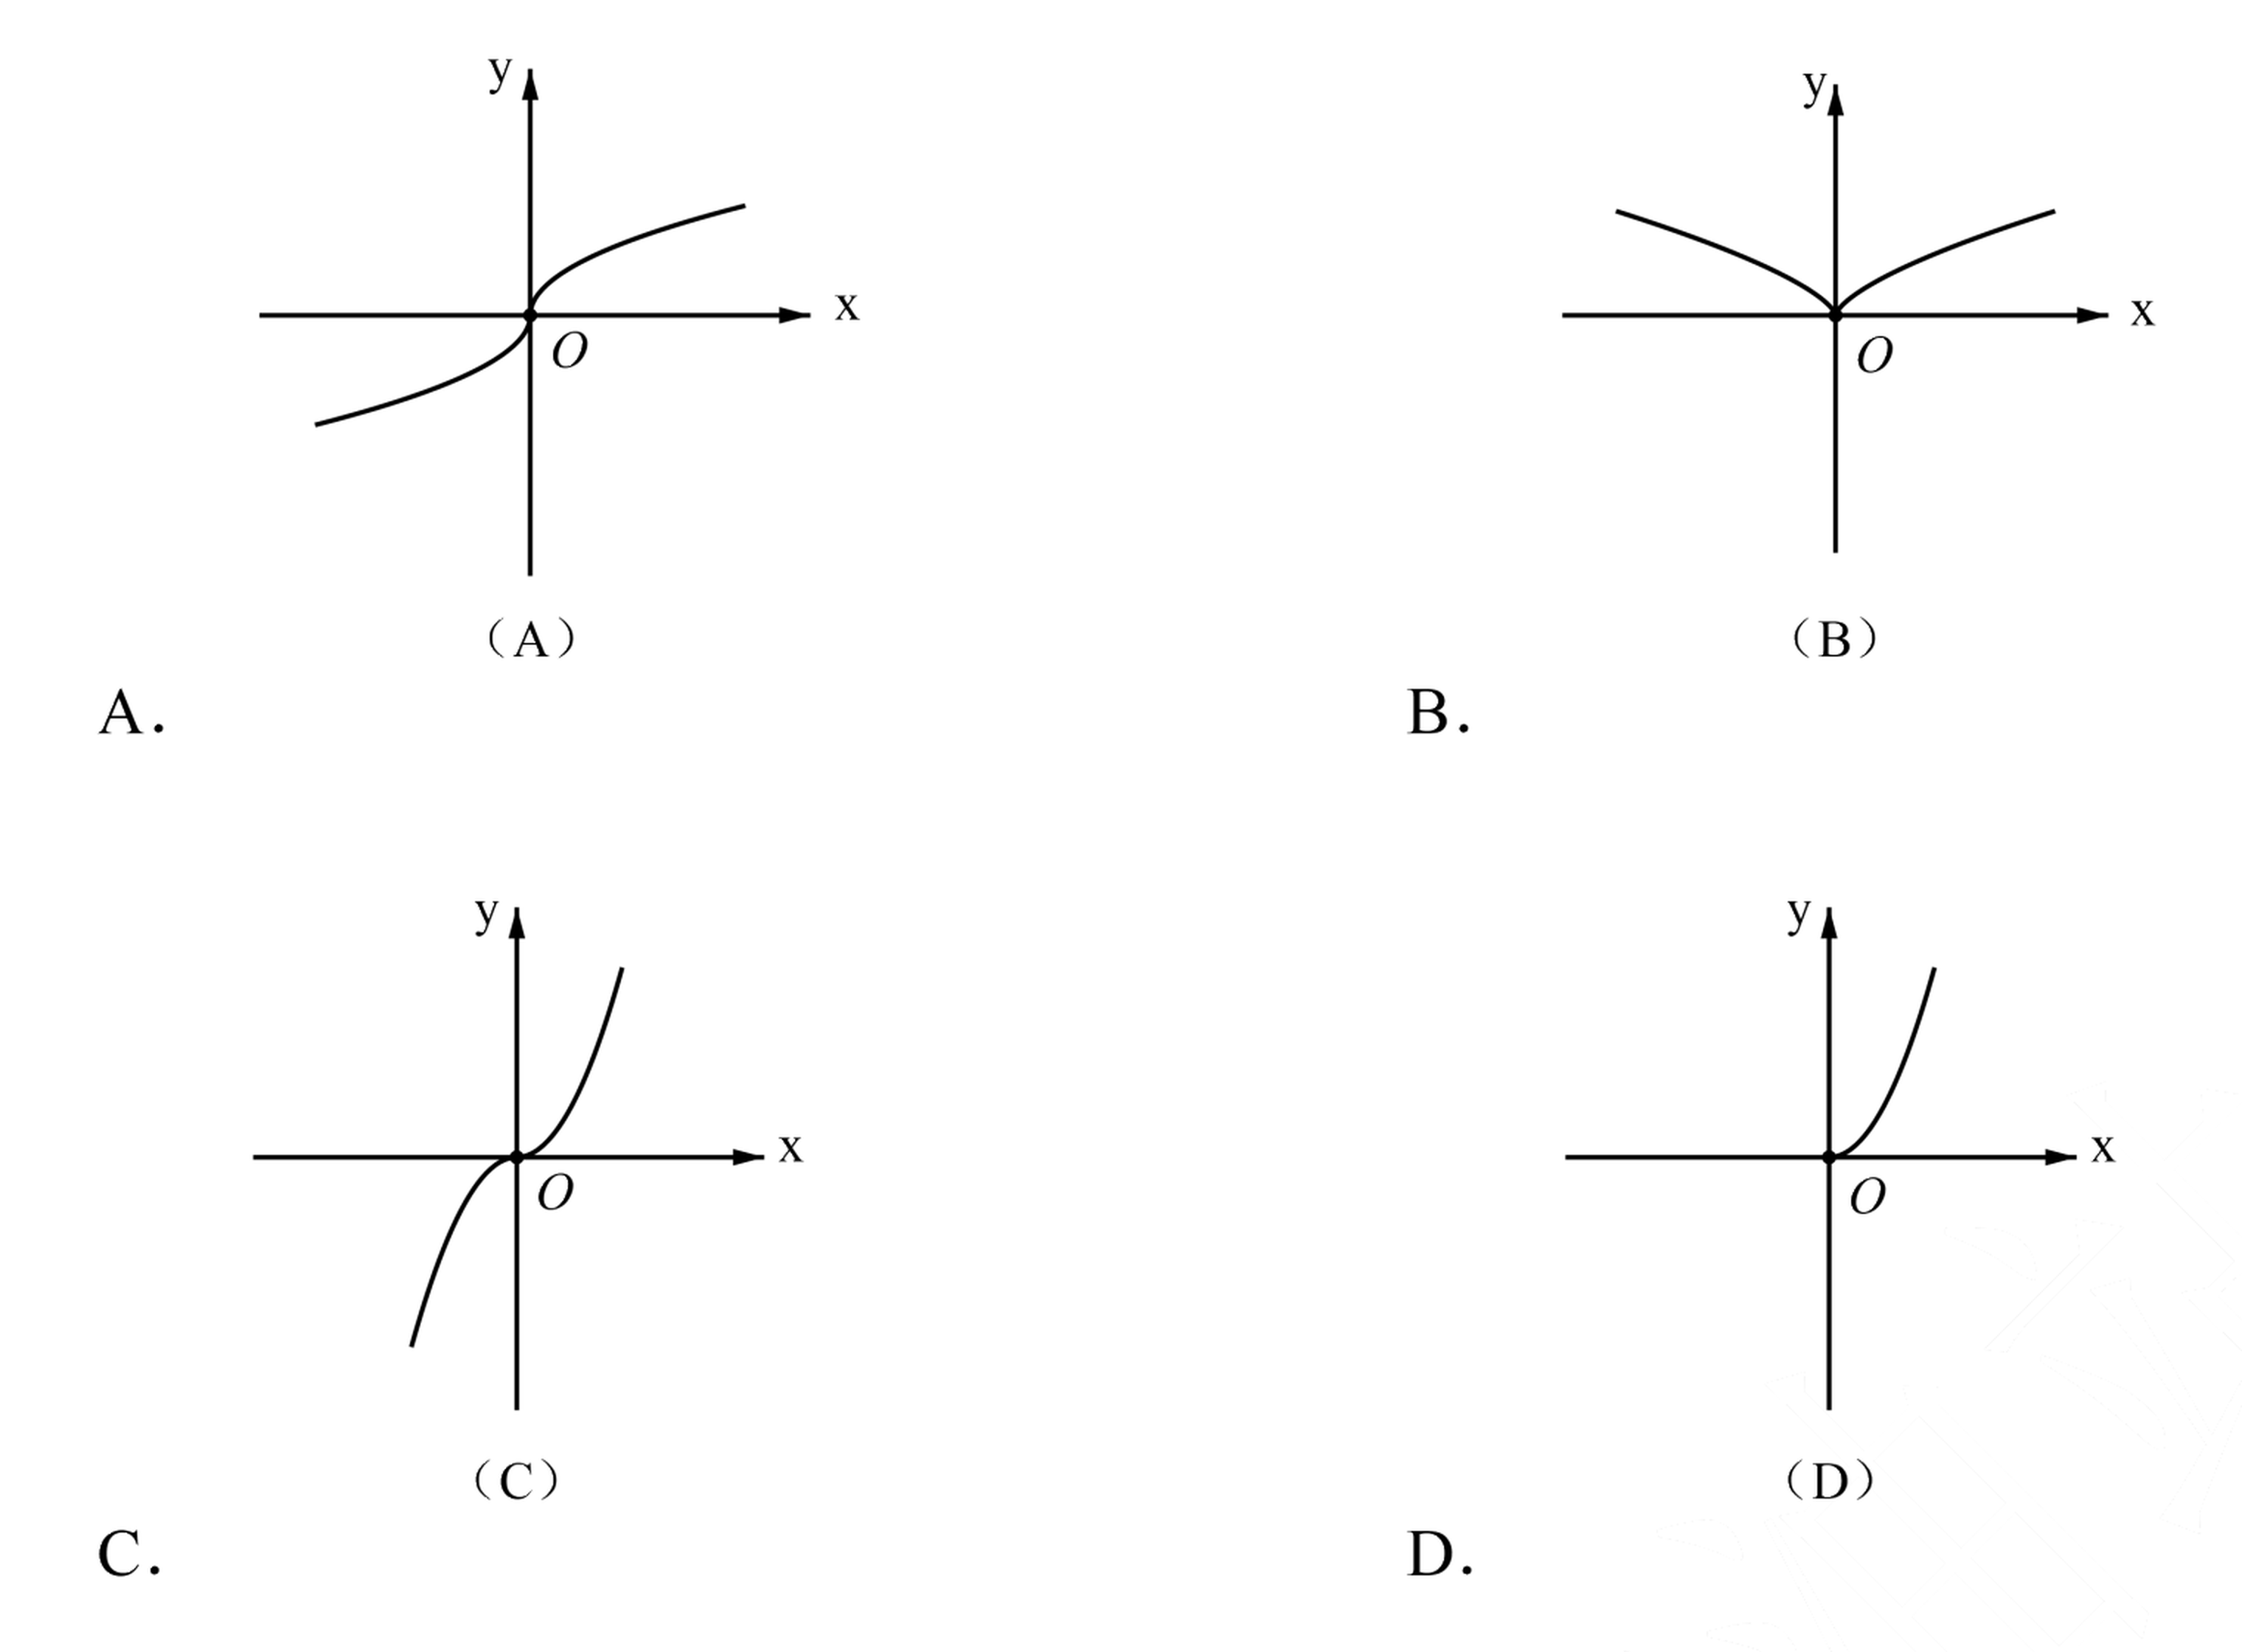
\includegraphics[width=0.80\textwidth]{figures/gao140_q14.png}
\end{center}

\ifanswer
\solbegin
\step{$f(x)=x^{\frac23}=\sqrt[3]{x^2}$ 是偶函数，且恒大于等于 $0$，故选 $B$.}
\solend
\fi

\item 设 $p$：关于 $x$ 的不等式 $x^2+ax+1>0$ 对 $x\in\R$ 恒成立，$q$：对数函数 $y=\log_{4-3a}x$ 在 $(0,+\infty)$ 上单调递减，那么 $p$ 是 $q$ 的\mbox{（\quad）}

\keepwithprev
A. 充分不必要条件\qquad B. 充要条件

C. 必要不充分条件\qquad D. 既不充分也不必要条件

\ifanswer
\solbegin
\step{$p\Leftrightarrow a^2-4<0\Leftrightarrow -2<a<2$. $q\Leftrightarrow 0<4-3a<1\Leftrightarrow 1<a<\dfrac43$.}
\step{由 $\left(1,\dfrac43\right)\subset(-2,2)$ 得 $q\Rightarrow p$；而 $a=0$ 时 $p$ 真、$q$ 假，}% 子集符号原卷印单线 $\subset$，照录
\step{故 $p$ 是 $q$ 的必要不充分条件，故选 $C$.}
\solend
\fi

\item “非空集合 $M$ 的元素都是集合 $P$ 的元素” 是假命题，现有下列命题：

(1) $M$ 的元素都不是 $P$ 的元素；(2) $M$ 中有不属于 $P$ 元素；% 原卷"不属于 P 元素"脱"的"字，照录

(3) $M$ 中有 $P$ 的元素；(4) $M$ 的元素不都是 $P$ 的元素，

其中真命题的个数是\mbox{（\quad）}

\keepwithprev
A. 1\qquad B. 2\qquad C. 3\qquad D. 4

\ifanswer
\solbegin
\step{由于 “非空集合 $M$ 的元素都是集合 $P$ 的元素” 是假命题，}
\step{得 “非空集合 $M$ 的元素至少有一个元素不属于集合 $P$” 是真命题.}
\step{则 (1) 不正确；(2) 正确；(3) $M$ 中不一定有 $P$ 的元素，例如 $M=\{a\}$，}
\step{则 $a\notin P$；(4) 正确.}
\step{综上，真命题只有 (2)(4). 故选 $B$.}
\solend
\fi

\end{enumerate}

\bigsec{三、解答题}

\begin{enumerate}
\setcounter{enumi}{16}

\item 设全集为 $\R$，集合 $A=\left\{x\mid\dfrac{2x}{x-1}\leqslant1\right\}$.

(1) 用区间表示集合 $A$；

(2) 若集合 $B=\{x\mid\lvert x+2\rvert+\lvert x-1\rvert=3\}$，求 $A\cup B$.

\ifanswer
\solbegin
\step{(1) 由 $\dfrac{2x}{x-1}\leqslant1\Leftrightarrow\dfrac{x+1}{x-1}\leqslant0$，故 $A=[-1,1)$，则 $\overline{A}=(-\infty,-1)\cup[1,+\infty)$；}
\step{(2) 由 $B=\{x\mid\lvert x+2\rvert+\lvert x-1\rvert=3\}=[-2,1]$，}
\step{结合上一问有 $A=[-1,1)$，所以 $A\cup B=B=[-2,1]$.}
\solend
\fi

\item (1) 已知指数函数 $y=a^x(a>0$ 且 $a\neq1)$ 在区间 $[-1,1]$ 上的最大值与最小值之和等于 $\dfrac52$，求实数 $a$ 的值.

(2) 已知幂函数 $y=x^{m^2+7m+10}(m\in\Z)$ 的图像关于 $y$ 轴对称，且在 $(0,+\infty)$ 上严格减. 若 $(a-1)^{m^2+7m+10}\geqslant(1+2a)^{m^2+7m+10}$. 求实数 $a$ 的取值范围.

\ifanswer
\solbegin
\step{(1) 指数函数 $y=a^x$ 在区间 $[-1,1]$ 上单调，所以 $a^1+a^{-1}=\dfrac52$，}
\step{所以 $a=2$ 或 $a=\dfrac12$；}
\step{(2) 由题意得 $m^2+7m+10<0$，所以 $-5<m<-2$，又因为 $m\in\Z$，}
\step{所以 $m=-4$ 或 $m=-3$，}
\step{当 $m=-4$ 时，$y=x^{m^2+7m+10}=x^{-2}$，为偶函数，}
\step{当 $m=-3$ 时，$y=x^{m^2+7m+10}=x^{-2}$，为偶函数，}
\step{所以 $m^2+7m+10=-2$，所以 $(a-1)^{-2}\geqslant(1+2a)^{-2}$，}
\step{所以 $\lvert a-1\rvert\leqslant\lvert 1+2a\rvert$，所以 $a\leqslant-2$ 或 $a\geqslant0$，所以 $a\in(-\infty,-2]\cup[0,+\infty)$.}
\solend
\fi

\item 设函数 $f(x)=ax^2+(1-a)x+a-2$ （$a\in\R$）.

(1) 若关于 $x$ 的不等式 $f(x)\leqslant0$ 的解集为 $\left[0,\dfrac12\right]$，求实数 $a$ 的值；

(2) 若 $a\geqslant0$，解关于 $x$ 的不等式：$f(x)<a-1$.

\ifanswer
\solbegin
\step{(1) 由解集得 $a>0$，且 $0$ 是方程 $f(x)=0$ 的根，故 $f(0)=a-2=0$，}
\step{得 $a=2$.}
\step{此时 $f(x)=2x^2-x=x(2x-1)$，$f(x)\leqslant0$ 的解集确为 $\left[0,\dfrac12\right]$.}
\step{(2) $f(x)<a-1\Leftrightarrow ax^2+(1-a)x-1<0\Leftrightarrow(x-1)(ax+1)<0$，}
\step{当 $a=0$ 时，$x-1<0$，解集为 $(-\infty,1)$.}
\step{当 $a>0$ 时，$-\dfrac1a<1$，解集为 $\left(-\dfrac1a,1\right)$.}
\solend
\fi

\item 为了保护环境，某单位采用新工艺，把二氧化碳转化为一种可利用的化工产品，已知该单位每月处理量最多不超过 $300$ 吨. 当月处理量为 $x$ 吨时，月处理成本为 $x^2-200x+40000(0<x\leqslant300)$ 元，且每处理一吨二氧化碳得到可利用的化工产品价值为 $300$ 元.

(1) 若要保证该单位每月不亏损，则每月处理量应控制在什么范围？

(2) 该单位每月处理量为多少吨时，才能使每吨的平均处理成本最低，最低为多少元？

\ifanswer
\solbegin
\step{(1) 由题意得 $S=300x-(x^2-200x+40000)$}
\step{$=-x^2+500x-40000(0<x\leqslant300)$，}
\step{令 $S\geqslant0$，即 $-x^2+500x-40000\geqslant0$，解得 $100\leqslant x\leqslant400$，}
\step{又 $0<x\leqslant300$，所以 $100\leqslant x\leqslant300$，}
\step{故要保证该单位每月不亏损，则每月处理量应控制在 $[100,300]$ 范围内；}
\step{(2) 每吨的平均出来成本为 $\dfrac yx=x+\dfrac{40000}x-200\geqslant2\sqrt{x\cdot\dfrac{40000}x}-200=200$，}% 原卷"平均出来成本"与题干"平均处理成本"措辞不一，照录
\step{当且仅当 $x=\dfrac{40000}x$，即 $x=200$ 时取等号，}
\step{所以该单位每月处理量为 $200$ 吨时，}
\step{才能使每吨的平均处理成本最低且最低为 $200$ 元.}
\solend
\fi

\item 已知函数 $y=f(x),x\in D$，若对于定义域 $D$ 内任意实数 $x,y$，不等式 $f(x)+f(y)\geqslant f(xy)$ 都成立，则称函数 $y=f(x)$ 是 $QB$ 函数，

(1) 判断函数 $f(x)=x+1$ 是否是 $QB$ 函数，并说明理由；

(2) 若函数 $g(x)=\ln(ax),x>0$ 是 $QB$ 函数，求实数 $a$ 的取值范围；

(3) 已知函数 $h(x)=a^x(a\in\R\text{ 且 }a>0)$，证明：“函数 $y=h(x)$ 是 $QB$ 函数” 的充要条件是 “ $a\in\{1\}$ ”.

\ifanswer
\solbegin
\step{(1) 不是，理由如下：因为 $f(x)=x+1$，}
\step{所以 $f(x)+f(y)\geqslant f(xy)\Leftrightarrow x+y\geqslant xy-1\Leftrightarrow(x-1)(y-1)\leqslant2$，}
\step{显然不恒成立，故不是 $QB$ 函数；}
\step{(2) 因为函数 $g(x)=\ln(ax),x>0$，则 $a>0$，}
\step{若函数 $g(x)$ 是 $QB$ 函数，则 $g(x)+g(y)\geqslant g(xy)$，}
\step{即 $\ln(ax)+\ln(ay)\geqslant\ln(axy)$，则 $\ln(a^2xy)\geqslant\ln(axy)$，得 $a^2xy\geqslant axy$，}
\step{且 $x>0,y>0$，得 $a^2\geqslant a$，解得 $a\geqslant1$ 或 $a\leqslant0$（舍去），}
\step{所以实数 $a$ 的取值范围为 $[1,+\infty)$.}
\step{(3) 若函数 $h(x)=a^x$ 是 $QB$ 函数，}
\step{当 $a>1$ 时，令 $x=y=\log_a\dfrac12$，则 $h(x)+h(y)=a^x+a^y=\dfrac12+\dfrac12=1$，}
\step{且 $h(xy)=a^{xy}=(a^x)^y=\left(\dfrac12\right)^{\log_a\frac12}=2^{\log_a2}$，}
\step{因为 $\log_a2>0$，所以 $h(xy)=2^{\log_a2}>1$，不满足 $h(x)+h(y)\geqslant h(xy)$，}
\step{不合题意；}
\step{当 $a=1$ 时，$h(x)+h(y)=a^x+a^y=1+1=2$，且 $h(xy)=a^{xy}=1$，}
\step{满足 $h(x)+h(y)\geqslant h(xy)$，符合题意；}
\step{当 $0<a<1$ 时，令 $x=\log_a2,y=2$，则 $h(x)+h(y)=a^x+a^y=2+a^2$，}
\step{且 $h(xy)=a^{xy}=(a^x)^y=2^2=4$，}
\step{因为 $0<a<1$，所以 $0<a^2<1$，得 $2<2+a^2<3$，}
\step{不满足 $h(x)+h(y)\geqslant h(xy)$，不合题意；}
\step{综上所述，$a\in\{1\}$，即充分性成立；}% 原卷"充分性/必要性"两标签与所证方向互换，照录
\step{若 $a\in\{1\}$，则 $h(x)+h(y)=a^x+a^y=1+1=2$，且 $h(xy)=a^{xy}=1$，}
\step{得 $h(x)+h(y)\geqslant h(xy)$，所以函数 $h(x)=a^x$ 是 $QB$ 函数，即必要性成立；}% 原卷"充分性/必要性"两标签与所证方向互换，照录
\step{综上所述，“函数 $y=h(x)$ 是 $QB$ 函数” 的充要条件是 “ $a\in\{1\}$ ”.}
\solend
\fi

\end{enumerate}

\end{document}
"
% 紧凑版：xelatex "\def\iscompact{1}% 高一140_甘泉外国语_期中.tex
%   —— 高一上数学"2026-2027 年甘泉外国语高一上期中"（试卷版/答案版）
% 试卷版：xelatex 高一140_甘泉外国语_期中.tex
% 答案版：xelatex "\def\isanswer{1}% 高一140_甘泉外国语_期中.tex
%   —— 高一上数学"2026-2027 年甘泉外国语高一上期中"（试卷版/答案版）
% 试卷版：xelatex 高一140_甘泉外国语_期中.tex
% 答案版：xelatex "\def\isanswer{1}\input{高一140_甘泉外国语_期中.tex}"
% 紧凑版：xelatex "\def\iscompact{1}\input{高一140_甘泉外国语_期中.tex}"
%
% ① 原始材料：微信公众号"魔都数学加油站"文章，连载"27学年高一140"，原文标题
% "27学年高一140——2026-2027年上海市甘泉外国语高一上期中"；
% 原文链接：https://mp.weixin.qq.com/s/eflgf2Ktk1LyT9x-k-ltLw。
% 正文为 9 张 PNG 页（01、02、03、05、06、07、08 为 4762x6735；04、09 为 2560x3620，
% 同一篇各页分辨率不同，逐页按各自分辨率裁图核对），题目下印有【答案】或【解析】，为讲评版。
% 题目、解析均据原图转录；卷面粉红色水印"魔都数学加油站"及公众号页脚未录入。
% 全卷 1 幅插图：第 14 题四幅坐标函数图象选项（04 页），取原卷截图去粉色水印、去色、
% LANCZOS 放大 2 倍，四幅选项按原卷 2x2 排布（含（A）（B）（C）（D）图注与 A./B./C./D.
% 选项字母）合并裁为一张；图前按惯例加 \needvspace 守卫。
%
% 卷首标题：原卷印作"2026-2027 年甘泉外国语高一上期中"（公众号标题中的"上海市"
% 卷面标题行没有，本稿照卷面），年份区间按全稿惯例排 en dash；原卷未印副标题，
% 本卷为期中卷、跨集合与常用逻辑用语／不等式／函数三章，按题目内容标为
% "集合与常用逻辑用语、不等式、函数"（与 125／126／128／129／131／132／133 同期中卷口径相同）：
% 集合与逻辑见 Q5、Q13、Q15、Q16、Q17，不等式见 Q3、Q10、Q11、Q19、Q20，
% 函数（指数／对数／幂函数及其图象、同构与 QB 函数）见 Q4、Q6、Q7、Q8、Q12、Q14、Q18、Q21。
%
% 题号体例：本卷共 19 题——一、填空题 3—12（10 题）、二、选择题 13—16（4 题）、
% 三、解答题 17—21（5 题）。三节分别 \setcounter{enumi}{2}／{12}／{16}。
% 原卷从第 3 题起、无第 1、2 题，本稿保留原题号。
%
% ② 与原卷的排版差异：
%   ① 原文从第 3 题起，本稿保留原题号；
%   ② 原卷每题下直接印【答案】或【解析】，本稿按全稿惯例置于答案版；第 5 题只印
%      【答案】、无【解析】，提 \ans{}；第 13、14、15、16 题答案均在【解析】末句
%      "故选 …"，题干括号内留空、不另提 \ans{}；其余各题印【解析】、无独立答案段；
%      全卷无"答案印在题干括号内且无解析"的一型；
%   ③ 原卷未印副标题，本稿按"知识模块"口径补出；
%   ④ 原卷填空横线按全稿惯例排为 \blankline[4.4em]；选择题括号排 \mbox{（\quad）}、
%      每个选项段前按惯例加 \keepwithprev（四幅图选项那一枚放在 \begin{center} 之前）；
%      解答题不留作答区、不加 \anspace（原卷为讲评版，与 129／131／132／133／136 同）；
%   ⑤ 原卷数集混排：斜体 $R$（Q9、Q12、Q15 等）与黑体／黑板粗体 $R$（Q15、Q17、
%      Q19、Q21）、粗体 $Z$（Q18），按全稿惯例统一改 \R／\Z；空集记号 \varnothing；
%      绝对值排 \lvert…\rvert，集合描述竖线排 \mid；不等号按全稿惯例排 \leqslant／\geqslant；
%      补集照原卷上划线排 \overline{A}；
%   ⑥ 子题标号 (1)(2)(3)(4) 原卷印半角括号，照录（与 131／132／133／134／136 同口径）；
%      括注原卷全角／半角混用，逐处照录：Q8"（结果用 a,b 表示）"、Q19"（a∈R）"、
%      Q21 (2)"（舍去）"印全角，Q18"$a^x(a>0$ 且 $a\neq1)$"、Q20"$40000(0<x\leqslant300)$"、
%      Q21 (3)"($a\in\R$ 且 $a>0$)"及 (0,+∞)、2(a>0) 等数学式内括注印半角；
%   ⑦ 数学式内半角逗号照录（如 Q8"$\lg2=a,10^b=3$"、Q11"$-2,3,4,\cdots,2027$"、
%      Q12"$x_1,x_2$"、Q19"$f(x)=ax^2+(1-a)x+a-2$"、Q21"$x>0,y>0$"）；
%      原卷行末西文句点照录（Q20 题干"300 吨. 当月处理量为 x 吨时"），行中全角逗号照录；
%   ⑧ 一幅插图：第 14 题四幅坐标函数图象选项合并裁为一张 \includegraphics
%      （题前 \needvspace{9cm}）。Q14 是"二、选择题"节内带大图块的第二题
%      （Q13 为节首题但无图），另在 \bigsec{二、选择题} 之前加 \needvspace{11cm}
%      连节标题一起量——守卫必须放在 \bigsec 之前，放标题之后会让"二、选择题"
%      孤立在页末（B 类，照 高一26／40／59／136 成例）；三版切页审计均"合计异常：无"；
%   ⑨ 跨页续印按题合并：Q9 题干在 01 页、解析续至 02 页；Q11 题干与解析前 3 行在 02 页、
%      后 2 行在 03 页；Q14 题干在 03 页末、四幅图与【解析】在 04 页；Q16 题干四条命题
%      在 04 页、选项与【解析】在 05 页；Q18 解析 (1) 首行在 05 页、其余 7 行在 06 页；
%      Q20 题干在 06 页末、"300 元."与两小问及【解析】在 07 页；Q21 解析跨 07—09 页
%      （末 3 行在 09 页）；本稿按题连排，不丢行；
%   ⑩ 题干中的中文弯引号按原卷照录，注释内一律 ASCII 引号；原卷"图像／图象"
%      两种写法混用，逐处照录（Q7、Q18 作"图像"，Q14 作"图象"）；
%   ⑪ 原卷无红色加粗标签（【解析】【答案】均黑色印刷），故本卷未用 \stepm。
%
% 判别式字形：全卷仅第 9 题【解析】"经验证得"cases 块出现两处判别式
%   "$\Delta=p^2-4q>0$"与"$\Delta'=q^2-4p>0$"，原卷两处均印等腰、偏高的
%   三角 $\Delta$（带撇的为 $\Delta'$），逐处放大核对并照录 \Delta、\Delta'；
%   全卷未出现扁等边三角 \triangle。
%
% 子集符号：第 15 题【解析】"由 (1,4/3)⊂(-2,2) 得 q⇒p"一处原卷印单线 $\subset$
%   （不带下划线），逐处放大核对、照录 \subset；全卷未出现带下划线的 \subseteq。
%
% 原卷存疑照录（均照录未改，正文对应处另有 % 注）：
%   第 16 题 (2) 命题"$M$ 中有不属于 $P$ 元素"中"不属于 $P$ 元素"脱"的"字，照录；
%   第 20 题题干 (2) 作"每吨的平均处理成本"、而【解析】(2) 作"每吨的平均出来成本"，
%      "出来"疑为"处理"之误，两处措辞照录不统一；
%   第 21 题 (3)【解析】"综上所述，$a\in\{1\}$，即充分性成立"与"即必要性成立"
%      两处标签与所证方向互换（按充要条件的通常口径），照录。
%
% 行数复核：一条 \step = 原卷解析的一个印刷行，cases 块作一个印刷行计。逐题数 \step
%   条数，合计 92 条（Q3：2；Q4：1；Q5：0；Q6：2；Q7：1；Q8：1；Q9：7；Q10：5；
%   Q11：5；Q12：4；Q13：6；Q14：1；Q15：3；Q16：5；Q17：3；Q18：8；Q19：6；
%   Q20：9；Q21：23），与原卷印刷行逐题相等。第 5 题只印【答案】、提 \ans{}，
%   不计入 \step 账；第 13、14、15、16 题答案在解析末句"故选 …"，括号内留空、
%   不另提 \ans{}；答案版【答案】/【解析】标记数 = 19（1 个 \ans + 18 个 \solbegin）
%   = 全卷题数。
%
\documentclass[a4paper,11pt]{article}
\usepackage{common}

\begin{document}

\examtitlest[3]{2026--2027 年甘泉外国语高一上期中}{集合与常用逻辑用语、不等式、函数}

\bigsec{一、填空题}

\begin{enumerate}
\setcounter{enumi}{2}

\item 不等式 $x^2-2x-3<0$ 的解集为\blankline[4.4em].

\ifanswer
\solbegin
\step{方程 $x^2-2x-3=0$ 的实数根是 $x_1=-1$，$x_2=3$；}
\step{所以不等式 $x^2-2x-3<0$ 的解集为 $\{x\mid -1<x<3\}$.}
\solend
\fi

\item 根式 $\sqrt{x\sqrt{x}}(x>0)$ 的指数幂形式为\blankline[4.4em].

\ifanswer
\solbegin
\step{$\sqrt{x\sqrt{x}}=\sqrt{x\cdot x^{\frac12}}=\sqrt{x^{\frac32}}=x^{\frac34}$.}
\solend
\fi

\item 陈述句 “ $x>1$ 或 $y>1$ ” 的否定形式是\blankline[4.4em].

\ifanswer
\ans{$x\leqslant1$ 且 $y\leqslant1$}
\fi

\item 若 $x<0$ 时，指数函数 $y=(a-1)^x$ 的值总大于 $1$，则实数 $a$ 的取值范围是\blankline[4.4em].

\ifanswer
\solbegin
\step{由题意得 $(a-1)^x>1$ 在 $(-\infty,0)$ 上恒成立，则 $0<a-1<1$，解得 $1<a<2$.}
\step{故实数 $a$ 的取值范围是 $(1,2)$.}
\solend
\fi

\item 若 $f(x)=\log_a(x-1)$，对任意 $a>0$ 且 $a\neq1$，函数 $y=f(x)$ 的图像必过定点\blankline[4.4em].

\ifanswer
\solbegin
\step{令 $x-1=1$，即 $x=2$，此时 $f(2)=0$，即函数图像过定点 $(2,0)$.}
\solend
\fi

\item 已知 $\lg 2=a,10^b=3$，则 $\log_6 2=$\blankline[4.4em]（结果用 $a,b$ 表示）.

\ifanswer
\solbegin
\step{由 $10^b=3$，得 $b=\lg 3$，则 $\log_6 2=\dfrac{\lg 2}{\lg 6}=\dfrac{\lg 2}{\lg 2+\lg 3}=\dfrac{a}{a+b}$.}
\solend
\fi

\item 已知 $p$、$q\in\R$，$x_1$、$x_2$ 是关于 $x$ 的方程 $x^2+px+q=0$ 的两实根，$x_1+1$、$x_2+1$ 是关于 $x$ 的方程 $x^2+qx+p=0$ 的两实根，则 $pq=$\blankline[4.4em].

\ifanswer
\solbegin
\step{因为 $x_1$、$x_2$ 是关于 $x$ 的方程 $x^2+px+q=0$ 的两实根，}
\step{由韦达定理得 $x_1+x_2=-p$，$x_1\cdot x_2=q$，}
\step{因为 $x_1+1$、$x_2+1$ 是关于 $x$ 的方程 $x^2+qx+p=0$ 的两实根，}
\step{由韦达定理得 $x_1+1+x_2+1=-q$，$(x_1+1)(x_2+1)=p$，}
\step{即 $x_1+x_2=-q-2$，$x_1+x_2+x_1x_2=p-1$，又 $x_1+x_2=-p$，$x_1\cdot x_2=q$，}
\step{所以 $\begin{cases}-p=-q-2\\-p+q=p-1\end{cases}$，解得 $\begin{cases}p=-1\\q=-3\end{cases}$，经验证得 $\begin{cases}\Delta=p^2-4q>0\\\Delta'=q^2-4p>0\end{cases}$，}% 判别式原卷印高三角 $\Delta$、$\Delta'$，照录
\step{则 $pq=3$.}
\solend
\fi

\item 对于 $x\in\R$，不等式 $\lvert 3-x\rvert+\lvert 1+x\rvert\geqslant a^2-3a$ 恒成立，则实数 $a$ 的取值范围是\blankline[4.4em].

\ifanswer
\solbegin
\step{对于 $x\in\R$，不等式 $\lvert 3-x\rvert+\lvert 1+x\rvert\geqslant a^2-3a$ 恒成立，}
\step{即 $\lvert 3-x\rvert+\lvert 1+x\rvert$ 的最小值大于或等于 $a^2-3a$，}
\step{$\lvert 3-x\rvert+\lvert 1+x\rvert$ 表示数轴上的 $x$ 对应点到 $3$ 和 $-1$ 对应点的距离之和，}
\step{它的最小值为 $4$，故 $4\geqslant a^2-3a$，即 $a^2-3a-4\leqslant0$，解得 $-1\leqslant a\leqslant4$，}
\step{故实数 $a$ 的取值范围是 $[-1,4]$.}
\solend
\fi

\item 已知同时满足不等式 $x^2-x-2>0$ 和 $2x^2+(5+2a)x+5a<0$ 的 $x$ 的整数值只有 $2026$ 个，则实数 $a$ 的取值范围是\blankline[4.4em].

\ifanswer
\solbegin
\step{整数 $x$ 须满足 $x\leqslant-2$ 或 $x\geqslant3$，且 $(2x+5)(x+a)<0$.}
\step{当 $a<\dfrac52$ 时，需使整数解恰为 $-2,3,4,\cdots,2027$，即 $2027<-a\leqslant2028$.}
\step{当 $a>\dfrac52$ 时，需使整数解恰为 $-2028,-2027,\cdots,-3$，即 $2028<a\leqslant2029$；}
\step{$a=\dfrac52$ 时无解.}
\step{故 $a\in[-2028,-2027)\cup(2028,2029]$.}
\solend
\fi

\item 同构式通俗讲是结构相同的表达式，如：$f(x)=x+e^x$，$f(\ln x)=\ln x+e^{\ln x}=\ln x+x$，称 $x+e^x$ 与 $\ln x+x$ 为同构式. 已知实数 $x_1,x_2$ 满足 $e^{x_1}+x_1=8,\ln\sqrt[5]{5x_2+3}+x_2=1$，则 $x_1+5x_2=$\blankline[4.4em].

\ifanswer
\solbegin
\step{函数 $f(x)=x+e^x$ 在 $\R$ 上严格增，且 $f(x_1)=x_1+e^{x_1}=8$，}
\step{由 $\ln\sqrt[5]{5x_2+3}+x_2=1$，得 $\ln(5x_2+3)+5x_2=5$，则 $\ln(5x_2+3)+5x_2+3=8$，}
\step{即 $f(\ln(5x_2+3))=8$，因此 $f(\ln(5x_2+3))=8=f(x_1)$，则 $x_1=\ln(5x_2+3)$，}
\step{所以 $x_1+5x_2=\ln(5x_2+3)+5x_2=5$.}
\solend
\fi

\end{enumerate}

% 第 14 题四幅图是"二、选择题"节内的大图块；守卫须放在 \bigsec 之前连节标题一起量，
% 否则"二、选择题"会孤立在页末（B 类，照 高一26／40／59／136 成例）
\needvspace{11cm}
\bigsec{二、选择题}

\begin{enumerate}
\setcounter{enumi}{12}

\item 设 $a$、$b$ 为实数，则 “ $a>b>0$ ” 的一个充分非必要条件是\mbox{（\quad）}

\keepwithprev
A. $\sqrt{a-1}>\sqrt{b-1}$\qquad B. $a^2>b^2$

C. $\dfrac1b>\dfrac1a$\qquad D. $a-b>b-a$

\ifanswer
\solbegin
\step{由 $\sqrt{a-1}>\sqrt{b-1}$ 得 $a>b\geqslant1$，故 $a>b>0$，反之不成立，满足题意；}
\step{由 $a^2>b^2$，则 $\lvert a\rvert>\lvert b\rvert$，推不出 $a>b>0$，反向可推出，不满足；}
\step{由 $\dfrac1b>\dfrac1a$，则 $a>b>0$ 或 $b>0>a$ 或 $0>a>b$，推不出 $a>b>0$，}
\step{反向可推出，不满足；}
\step{由 $a-b>b-a$，则 $a>b$，推不出 $a>b>0$，反向可推出，不满足；}
\step{故选 $A$.}
\solend
\fi

% 第 14 题四幅坐标函数图象选项是一整块，守卫放在 \item 之前
\needvspace{9cm}
\item 幂函数 $f(x)=x^{\frac23}$ 的图象大致为\mbox{（\quad）}

\keepwithprev
\begin{center}
% 四幅坐标函数图象选项取原卷 04 页截图去粉色水印、去色，按原卷 2x2 排布合并为一张
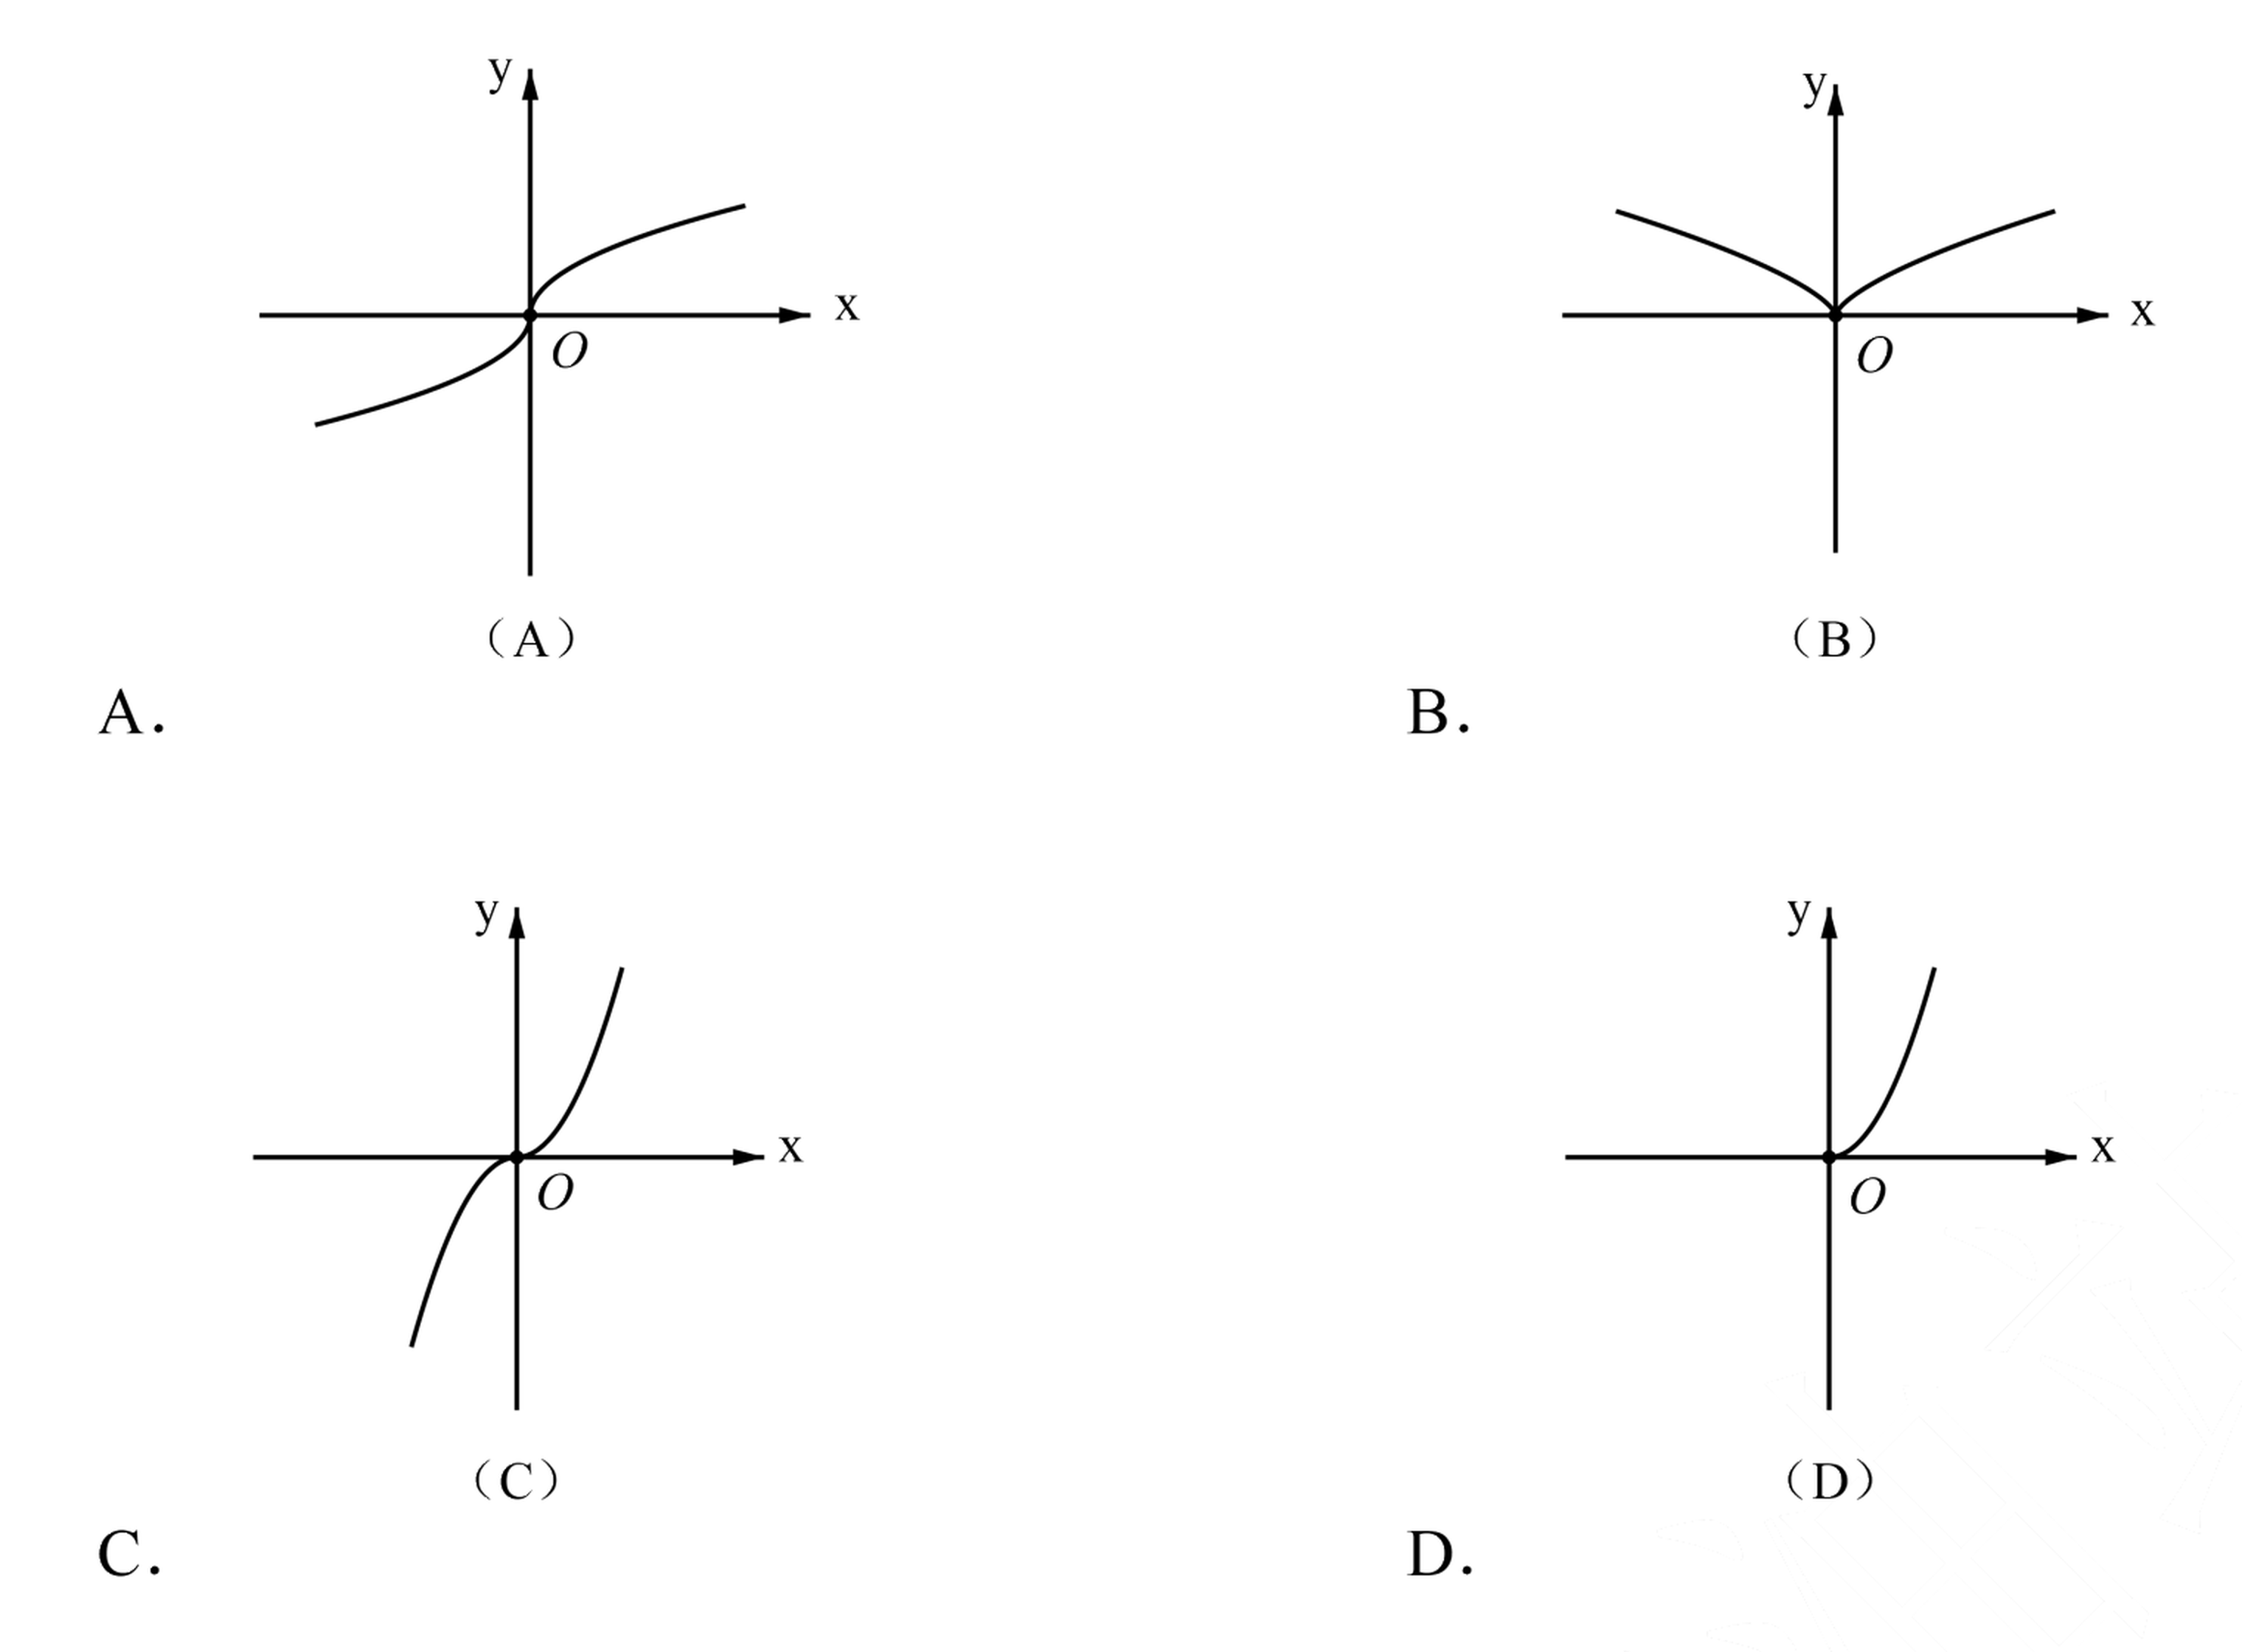
\includegraphics[width=0.80\textwidth]{figures/gao140_q14.png}
\end{center}

\ifanswer
\solbegin
\step{$f(x)=x^{\frac23}=\sqrt[3]{x^2}$ 是偶函数，且恒大于等于 $0$，故选 $B$.}
\solend
\fi

\item 设 $p$：关于 $x$ 的不等式 $x^2+ax+1>0$ 对 $x\in\R$ 恒成立，$q$：对数函数 $y=\log_{4-3a}x$ 在 $(0,+\infty)$ 上单调递减，那么 $p$ 是 $q$ 的\mbox{（\quad）}

\keepwithprev
A. 充分不必要条件\qquad B. 充要条件

C. 必要不充分条件\qquad D. 既不充分也不必要条件

\ifanswer
\solbegin
\step{$p\Leftrightarrow a^2-4<0\Leftrightarrow -2<a<2$. $q\Leftrightarrow 0<4-3a<1\Leftrightarrow 1<a<\dfrac43$.}
\step{由 $\left(1,\dfrac43\right)\subset(-2,2)$ 得 $q\Rightarrow p$；而 $a=0$ 时 $p$ 真、$q$ 假，}% 子集符号原卷印单线 $\subset$，照录
\step{故 $p$ 是 $q$ 的必要不充分条件，故选 $C$.}
\solend
\fi

\item “非空集合 $M$ 的元素都是集合 $P$ 的元素” 是假命题，现有下列命题：

(1) $M$ 的元素都不是 $P$ 的元素；(2) $M$ 中有不属于 $P$ 元素；% 原卷"不属于 P 元素"脱"的"字，照录

(3) $M$ 中有 $P$ 的元素；(4) $M$ 的元素不都是 $P$ 的元素，

其中真命题的个数是\mbox{（\quad）}

\keepwithprev
A. 1\qquad B. 2\qquad C. 3\qquad D. 4

\ifanswer
\solbegin
\step{由于 “非空集合 $M$ 的元素都是集合 $P$ 的元素” 是假命题，}
\step{得 “非空集合 $M$ 的元素至少有一个元素不属于集合 $P$” 是真命题.}
\step{则 (1) 不正确；(2) 正确；(3) $M$ 中不一定有 $P$ 的元素，例如 $M=\{a\}$，}
\step{则 $a\notin P$；(4) 正确.}
\step{综上，真命题只有 (2)(4). 故选 $B$.}
\solend
\fi

\end{enumerate}

\bigsec{三、解答题}

\begin{enumerate}
\setcounter{enumi}{16}

\item 设全集为 $\R$，集合 $A=\left\{x\mid\dfrac{2x}{x-1}\leqslant1\right\}$.

(1) 用区间表示集合 $A$；

(2) 若集合 $B=\{x\mid\lvert x+2\rvert+\lvert x-1\rvert=3\}$，求 $A\cup B$.

\ifanswer
\solbegin
\step{(1) 由 $\dfrac{2x}{x-1}\leqslant1\Leftrightarrow\dfrac{x+1}{x-1}\leqslant0$，故 $A=[-1,1)$，则 $\overline{A}=(-\infty,-1)\cup[1,+\infty)$；}
\step{(2) 由 $B=\{x\mid\lvert x+2\rvert+\lvert x-1\rvert=3\}=[-2,1]$，}
\step{结合上一问有 $A=[-1,1)$，所以 $A\cup B=B=[-2,1]$.}
\solend
\fi

\item (1) 已知指数函数 $y=a^x(a>0$ 且 $a\neq1)$ 在区间 $[-1,1]$ 上的最大值与最小值之和等于 $\dfrac52$，求实数 $a$ 的值.

(2) 已知幂函数 $y=x^{m^2+7m+10}(m\in\Z)$ 的图像关于 $y$ 轴对称，且在 $(0,+\infty)$ 上严格减. 若 $(a-1)^{m^2+7m+10}\geqslant(1+2a)^{m^2+7m+10}$. 求实数 $a$ 的取值范围.

\ifanswer
\solbegin
\step{(1) 指数函数 $y=a^x$ 在区间 $[-1,1]$ 上单调，所以 $a^1+a^{-1}=\dfrac52$，}
\step{所以 $a=2$ 或 $a=\dfrac12$；}
\step{(2) 由题意得 $m^2+7m+10<0$，所以 $-5<m<-2$，又因为 $m\in\Z$，}
\step{所以 $m=-4$ 或 $m=-3$，}
\step{当 $m=-4$ 时，$y=x^{m^2+7m+10}=x^{-2}$，为偶函数，}
\step{当 $m=-3$ 时，$y=x^{m^2+7m+10}=x^{-2}$，为偶函数，}
\step{所以 $m^2+7m+10=-2$，所以 $(a-1)^{-2}\geqslant(1+2a)^{-2}$，}
\step{所以 $\lvert a-1\rvert\leqslant\lvert 1+2a\rvert$，所以 $a\leqslant-2$ 或 $a\geqslant0$，所以 $a\in(-\infty,-2]\cup[0,+\infty)$.}
\solend
\fi

\item 设函数 $f(x)=ax^2+(1-a)x+a-2$ （$a\in\R$）.

(1) 若关于 $x$ 的不等式 $f(x)\leqslant0$ 的解集为 $\left[0,\dfrac12\right]$，求实数 $a$ 的值；

(2) 若 $a\geqslant0$，解关于 $x$ 的不等式：$f(x)<a-1$.

\ifanswer
\solbegin
\step{(1) 由解集得 $a>0$，且 $0$ 是方程 $f(x)=0$ 的根，故 $f(0)=a-2=0$，}
\step{得 $a=2$.}
\step{此时 $f(x)=2x^2-x=x(2x-1)$，$f(x)\leqslant0$ 的解集确为 $\left[0,\dfrac12\right]$.}
\step{(2) $f(x)<a-1\Leftrightarrow ax^2+(1-a)x-1<0\Leftrightarrow(x-1)(ax+1)<0$，}
\step{当 $a=0$ 时，$x-1<0$，解集为 $(-\infty,1)$.}
\step{当 $a>0$ 时，$-\dfrac1a<1$，解集为 $\left(-\dfrac1a,1\right)$.}
\solend
\fi

\item 为了保护环境，某单位采用新工艺，把二氧化碳转化为一种可利用的化工产品，已知该单位每月处理量最多不超过 $300$ 吨. 当月处理量为 $x$ 吨时，月处理成本为 $x^2-200x+40000(0<x\leqslant300)$ 元，且每处理一吨二氧化碳得到可利用的化工产品价值为 $300$ 元.

(1) 若要保证该单位每月不亏损，则每月处理量应控制在什么范围？

(2) 该单位每月处理量为多少吨时，才能使每吨的平均处理成本最低，最低为多少元？

\ifanswer
\solbegin
\step{(1) 由题意得 $S=300x-(x^2-200x+40000)$}
\step{$=-x^2+500x-40000(0<x\leqslant300)$，}
\step{令 $S\geqslant0$，即 $-x^2+500x-40000\geqslant0$，解得 $100\leqslant x\leqslant400$，}
\step{又 $0<x\leqslant300$，所以 $100\leqslant x\leqslant300$，}
\step{故要保证该单位每月不亏损，则每月处理量应控制在 $[100,300]$ 范围内；}
\step{(2) 每吨的平均出来成本为 $\dfrac yx=x+\dfrac{40000}x-200\geqslant2\sqrt{x\cdot\dfrac{40000}x}-200=200$，}% 原卷"平均出来成本"与题干"平均处理成本"措辞不一，照录
\step{当且仅当 $x=\dfrac{40000}x$，即 $x=200$ 时取等号，}
\step{所以该单位每月处理量为 $200$ 吨时，}
\step{才能使每吨的平均处理成本最低且最低为 $200$ 元.}
\solend
\fi

\item 已知函数 $y=f(x),x\in D$，若对于定义域 $D$ 内任意实数 $x,y$，不等式 $f(x)+f(y)\geqslant f(xy)$ 都成立，则称函数 $y=f(x)$ 是 $QB$ 函数，

(1) 判断函数 $f(x)=x+1$ 是否是 $QB$ 函数，并说明理由；

(2) 若函数 $g(x)=\ln(ax),x>0$ 是 $QB$ 函数，求实数 $a$ 的取值范围；

(3) 已知函数 $h(x)=a^x(a\in\R\text{ 且 }a>0)$，证明：“函数 $y=h(x)$ 是 $QB$ 函数” 的充要条件是 “ $a\in\{1\}$ ”.

\ifanswer
\solbegin
\step{(1) 不是，理由如下：因为 $f(x)=x+1$，}
\step{所以 $f(x)+f(y)\geqslant f(xy)\Leftrightarrow x+y\geqslant xy-1\Leftrightarrow(x-1)(y-1)\leqslant2$，}
\step{显然不恒成立，故不是 $QB$ 函数；}
\step{(2) 因为函数 $g(x)=\ln(ax),x>0$，则 $a>0$，}
\step{若函数 $g(x)$ 是 $QB$ 函数，则 $g(x)+g(y)\geqslant g(xy)$，}
\step{即 $\ln(ax)+\ln(ay)\geqslant\ln(axy)$，则 $\ln(a^2xy)\geqslant\ln(axy)$，得 $a^2xy\geqslant axy$，}
\step{且 $x>0,y>0$，得 $a^2\geqslant a$，解得 $a\geqslant1$ 或 $a\leqslant0$（舍去），}
\step{所以实数 $a$ 的取值范围为 $[1,+\infty)$.}
\step{(3) 若函数 $h(x)=a^x$ 是 $QB$ 函数，}
\step{当 $a>1$ 时，令 $x=y=\log_a\dfrac12$，则 $h(x)+h(y)=a^x+a^y=\dfrac12+\dfrac12=1$，}
\step{且 $h(xy)=a^{xy}=(a^x)^y=\left(\dfrac12\right)^{\log_a\frac12}=2^{\log_a2}$，}
\step{因为 $\log_a2>0$，所以 $h(xy)=2^{\log_a2}>1$，不满足 $h(x)+h(y)\geqslant h(xy)$，}
\step{不合题意；}
\step{当 $a=1$ 时，$h(x)+h(y)=a^x+a^y=1+1=2$，且 $h(xy)=a^{xy}=1$，}
\step{满足 $h(x)+h(y)\geqslant h(xy)$，符合题意；}
\step{当 $0<a<1$ 时，令 $x=\log_a2,y=2$，则 $h(x)+h(y)=a^x+a^y=2+a^2$，}
\step{且 $h(xy)=a^{xy}=(a^x)^y=2^2=4$，}
\step{因为 $0<a<1$，所以 $0<a^2<1$，得 $2<2+a^2<3$，}
\step{不满足 $h(x)+h(y)\geqslant h(xy)$，不合题意；}
\step{综上所述，$a\in\{1\}$，即充分性成立；}% 原卷"充分性/必要性"两标签与所证方向互换，照录
\step{若 $a\in\{1\}$，则 $h(x)+h(y)=a^x+a^y=1+1=2$，且 $h(xy)=a^{xy}=1$，}
\step{得 $h(x)+h(y)\geqslant h(xy)$，所以函数 $h(x)=a^x$ 是 $QB$ 函数，即必要性成立；}% 原卷"充分性/必要性"两标签与所证方向互换，照录
\step{综上所述，“函数 $y=h(x)$ 是 $QB$ 函数” 的充要条件是 “ $a\in\{1\}$ ”.}
\solend
\fi

\end{enumerate}

\end{document}
"
% 紧凑版：xelatex "\def\iscompact{1}% 高一140_甘泉外国语_期中.tex
%   —— 高一上数学"2026-2027 年甘泉外国语高一上期中"（试卷版/答案版）
% 试卷版：xelatex 高一140_甘泉外国语_期中.tex
% 答案版：xelatex "\def\isanswer{1}\input{高一140_甘泉外国语_期中.tex}"
% 紧凑版：xelatex "\def\iscompact{1}\input{高一140_甘泉外国语_期中.tex}"
%
% ① 原始材料：微信公众号"魔都数学加油站"文章，连载"27学年高一140"，原文标题
% "27学年高一140——2026-2027年上海市甘泉外国语高一上期中"；
% 原文链接：https://mp.weixin.qq.com/s/eflgf2Ktk1LyT9x-k-ltLw。
% 正文为 9 张 PNG 页（01、02、03、05、06、07、08 为 4762x6735；04、09 为 2560x3620，
% 同一篇各页分辨率不同，逐页按各自分辨率裁图核对），题目下印有【答案】或【解析】，为讲评版。
% 题目、解析均据原图转录；卷面粉红色水印"魔都数学加油站"及公众号页脚未录入。
% 全卷 1 幅插图：第 14 题四幅坐标函数图象选项（04 页），取原卷截图去粉色水印、去色、
% LANCZOS 放大 2 倍，四幅选项按原卷 2x2 排布（含（A）（B）（C）（D）图注与 A./B./C./D.
% 选项字母）合并裁为一张；图前按惯例加 \needvspace 守卫。
%
% 卷首标题：原卷印作"2026-2027 年甘泉外国语高一上期中"（公众号标题中的"上海市"
% 卷面标题行没有，本稿照卷面），年份区间按全稿惯例排 en dash；原卷未印副标题，
% 本卷为期中卷、跨集合与常用逻辑用语／不等式／函数三章，按题目内容标为
% "集合与常用逻辑用语、不等式、函数"（与 125／126／128／129／131／132／133 同期中卷口径相同）：
% 集合与逻辑见 Q5、Q13、Q15、Q16、Q17，不等式见 Q3、Q10、Q11、Q19、Q20，
% 函数（指数／对数／幂函数及其图象、同构与 QB 函数）见 Q4、Q6、Q7、Q8、Q12、Q14、Q18、Q21。
%
% 题号体例：本卷共 19 题——一、填空题 3—12（10 题）、二、选择题 13—16（4 题）、
% 三、解答题 17—21（5 题）。三节分别 \setcounter{enumi}{2}／{12}／{16}。
% 原卷从第 3 题起、无第 1、2 题，本稿保留原题号。
%
% ② 与原卷的排版差异：
%   ① 原文从第 3 题起，本稿保留原题号；
%   ② 原卷每题下直接印【答案】或【解析】，本稿按全稿惯例置于答案版；第 5 题只印
%      【答案】、无【解析】，提 \ans{}；第 13、14、15、16 题答案均在【解析】末句
%      "故选 …"，题干括号内留空、不另提 \ans{}；其余各题印【解析】、无独立答案段；
%      全卷无"答案印在题干括号内且无解析"的一型；
%   ③ 原卷未印副标题，本稿按"知识模块"口径补出；
%   ④ 原卷填空横线按全稿惯例排为 \blankline[4.4em]；选择题括号排 \mbox{（\quad）}、
%      每个选项段前按惯例加 \keepwithprev（四幅图选项那一枚放在 \begin{center} 之前）；
%      解答题不留作答区、不加 \anspace（原卷为讲评版，与 129／131／132／133／136 同）；
%   ⑤ 原卷数集混排：斜体 $R$（Q9、Q12、Q15 等）与黑体／黑板粗体 $R$（Q15、Q17、
%      Q19、Q21）、粗体 $Z$（Q18），按全稿惯例统一改 \R／\Z；空集记号 \varnothing；
%      绝对值排 \lvert…\rvert，集合描述竖线排 \mid；不等号按全稿惯例排 \leqslant／\geqslant；
%      补集照原卷上划线排 \overline{A}；
%   ⑥ 子题标号 (1)(2)(3)(4) 原卷印半角括号，照录（与 131／132／133／134／136 同口径）；
%      括注原卷全角／半角混用，逐处照录：Q8"（结果用 a,b 表示）"、Q19"（a∈R）"、
%      Q21 (2)"（舍去）"印全角，Q18"$a^x(a>0$ 且 $a\neq1)$"、Q20"$40000(0<x\leqslant300)$"、
%      Q21 (3)"($a\in\R$ 且 $a>0$)"及 (0,+∞)、2(a>0) 等数学式内括注印半角；
%   ⑦ 数学式内半角逗号照录（如 Q8"$\lg2=a,10^b=3$"、Q11"$-2,3,4,\cdots,2027$"、
%      Q12"$x_1,x_2$"、Q19"$f(x)=ax^2+(1-a)x+a-2$"、Q21"$x>0,y>0$"）；
%      原卷行末西文句点照录（Q20 题干"300 吨. 当月处理量为 x 吨时"），行中全角逗号照录；
%   ⑧ 一幅插图：第 14 题四幅坐标函数图象选项合并裁为一张 \includegraphics
%      （题前 \needvspace{9cm}）。Q14 是"二、选择题"节内带大图块的第二题
%      （Q13 为节首题但无图），另在 \bigsec{二、选择题} 之前加 \needvspace{11cm}
%      连节标题一起量——守卫必须放在 \bigsec 之前，放标题之后会让"二、选择题"
%      孤立在页末（B 类，照 高一26／40／59／136 成例）；三版切页审计均"合计异常：无"；
%   ⑨ 跨页续印按题合并：Q9 题干在 01 页、解析续至 02 页；Q11 题干与解析前 3 行在 02 页、
%      后 2 行在 03 页；Q14 题干在 03 页末、四幅图与【解析】在 04 页；Q16 题干四条命题
%      在 04 页、选项与【解析】在 05 页；Q18 解析 (1) 首行在 05 页、其余 7 行在 06 页；
%      Q20 题干在 06 页末、"300 元."与两小问及【解析】在 07 页；Q21 解析跨 07—09 页
%      （末 3 行在 09 页）；本稿按题连排，不丢行；
%   ⑩ 题干中的中文弯引号按原卷照录，注释内一律 ASCII 引号；原卷"图像／图象"
%      两种写法混用，逐处照录（Q7、Q18 作"图像"，Q14 作"图象"）；
%   ⑪ 原卷无红色加粗标签（【解析】【答案】均黑色印刷），故本卷未用 \stepm。
%
% 判别式字形：全卷仅第 9 题【解析】"经验证得"cases 块出现两处判别式
%   "$\Delta=p^2-4q>0$"与"$\Delta'=q^2-4p>0$"，原卷两处均印等腰、偏高的
%   三角 $\Delta$（带撇的为 $\Delta'$），逐处放大核对并照录 \Delta、\Delta'；
%   全卷未出现扁等边三角 \triangle。
%
% 子集符号：第 15 题【解析】"由 (1,4/3)⊂(-2,2) 得 q⇒p"一处原卷印单线 $\subset$
%   （不带下划线），逐处放大核对、照录 \subset；全卷未出现带下划线的 \subseteq。
%
% 原卷存疑照录（均照录未改，正文对应处另有 % 注）：
%   第 16 题 (2) 命题"$M$ 中有不属于 $P$ 元素"中"不属于 $P$ 元素"脱"的"字，照录；
%   第 20 题题干 (2) 作"每吨的平均处理成本"、而【解析】(2) 作"每吨的平均出来成本"，
%      "出来"疑为"处理"之误，两处措辞照录不统一；
%   第 21 题 (3)【解析】"综上所述，$a\in\{1\}$，即充分性成立"与"即必要性成立"
%      两处标签与所证方向互换（按充要条件的通常口径），照录。
%
% 行数复核：一条 \step = 原卷解析的一个印刷行，cases 块作一个印刷行计。逐题数 \step
%   条数，合计 92 条（Q3：2；Q4：1；Q5：0；Q6：2；Q7：1；Q8：1；Q9：7；Q10：5；
%   Q11：5；Q12：4；Q13：6；Q14：1；Q15：3；Q16：5；Q17：3；Q18：8；Q19：6；
%   Q20：9；Q21：23），与原卷印刷行逐题相等。第 5 题只印【答案】、提 \ans{}，
%   不计入 \step 账；第 13、14、15、16 题答案在解析末句"故选 …"，括号内留空、
%   不另提 \ans{}；答案版【答案】/【解析】标记数 = 19（1 个 \ans + 18 个 \solbegin）
%   = 全卷题数。
%
\documentclass[a4paper,11pt]{article}
\usepackage{common}

\begin{document}

\examtitlest[3]{2026--2027 年甘泉外国语高一上期中}{集合与常用逻辑用语、不等式、函数}

\bigsec{一、填空题}

\begin{enumerate}
\setcounter{enumi}{2}

\item 不等式 $x^2-2x-3<0$ 的解集为\blankline[4.4em].

\ifanswer
\solbegin
\step{方程 $x^2-2x-3=0$ 的实数根是 $x_1=-1$，$x_2=3$；}
\step{所以不等式 $x^2-2x-3<0$ 的解集为 $\{x\mid -1<x<3\}$.}
\solend
\fi

\item 根式 $\sqrt{x\sqrt{x}}(x>0)$ 的指数幂形式为\blankline[4.4em].

\ifanswer
\solbegin
\step{$\sqrt{x\sqrt{x}}=\sqrt{x\cdot x^{\frac12}}=\sqrt{x^{\frac32}}=x^{\frac34}$.}
\solend
\fi

\item 陈述句 “ $x>1$ 或 $y>1$ ” 的否定形式是\blankline[4.4em].

\ifanswer
\ans{$x\leqslant1$ 且 $y\leqslant1$}
\fi

\item 若 $x<0$ 时，指数函数 $y=(a-1)^x$ 的值总大于 $1$，则实数 $a$ 的取值范围是\blankline[4.4em].

\ifanswer
\solbegin
\step{由题意得 $(a-1)^x>1$ 在 $(-\infty,0)$ 上恒成立，则 $0<a-1<1$，解得 $1<a<2$.}
\step{故实数 $a$ 的取值范围是 $(1,2)$.}
\solend
\fi

\item 若 $f(x)=\log_a(x-1)$，对任意 $a>0$ 且 $a\neq1$，函数 $y=f(x)$ 的图像必过定点\blankline[4.4em].

\ifanswer
\solbegin
\step{令 $x-1=1$，即 $x=2$，此时 $f(2)=0$，即函数图像过定点 $(2,0)$.}
\solend
\fi

\item 已知 $\lg 2=a,10^b=3$，则 $\log_6 2=$\blankline[4.4em]（结果用 $a,b$ 表示）.

\ifanswer
\solbegin
\step{由 $10^b=3$，得 $b=\lg 3$，则 $\log_6 2=\dfrac{\lg 2}{\lg 6}=\dfrac{\lg 2}{\lg 2+\lg 3}=\dfrac{a}{a+b}$.}
\solend
\fi

\item 已知 $p$、$q\in\R$，$x_1$、$x_2$ 是关于 $x$ 的方程 $x^2+px+q=0$ 的两实根，$x_1+1$、$x_2+1$ 是关于 $x$ 的方程 $x^2+qx+p=0$ 的两实根，则 $pq=$\blankline[4.4em].

\ifanswer
\solbegin
\step{因为 $x_1$、$x_2$ 是关于 $x$ 的方程 $x^2+px+q=0$ 的两实根，}
\step{由韦达定理得 $x_1+x_2=-p$，$x_1\cdot x_2=q$，}
\step{因为 $x_1+1$、$x_2+1$ 是关于 $x$ 的方程 $x^2+qx+p=0$ 的两实根，}
\step{由韦达定理得 $x_1+1+x_2+1=-q$，$(x_1+1)(x_2+1)=p$，}
\step{即 $x_1+x_2=-q-2$，$x_1+x_2+x_1x_2=p-1$，又 $x_1+x_2=-p$，$x_1\cdot x_2=q$，}
\step{所以 $\begin{cases}-p=-q-2\\-p+q=p-1\end{cases}$，解得 $\begin{cases}p=-1\\q=-3\end{cases}$，经验证得 $\begin{cases}\Delta=p^2-4q>0\\\Delta'=q^2-4p>0\end{cases}$，}% 判别式原卷印高三角 $\Delta$、$\Delta'$，照录
\step{则 $pq=3$.}
\solend
\fi

\item 对于 $x\in\R$，不等式 $\lvert 3-x\rvert+\lvert 1+x\rvert\geqslant a^2-3a$ 恒成立，则实数 $a$ 的取值范围是\blankline[4.4em].

\ifanswer
\solbegin
\step{对于 $x\in\R$，不等式 $\lvert 3-x\rvert+\lvert 1+x\rvert\geqslant a^2-3a$ 恒成立，}
\step{即 $\lvert 3-x\rvert+\lvert 1+x\rvert$ 的最小值大于或等于 $a^2-3a$，}
\step{$\lvert 3-x\rvert+\lvert 1+x\rvert$ 表示数轴上的 $x$ 对应点到 $3$ 和 $-1$ 对应点的距离之和，}
\step{它的最小值为 $4$，故 $4\geqslant a^2-3a$，即 $a^2-3a-4\leqslant0$，解得 $-1\leqslant a\leqslant4$，}
\step{故实数 $a$ 的取值范围是 $[-1,4]$.}
\solend
\fi

\item 已知同时满足不等式 $x^2-x-2>0$ 和 $2x^2+(5+2a)x+5a<0$ 的 $x$ 的整数值只有 $2026$ 个，则实数 $a$ 的取值范围是\blankline[4.4em].

\ifanswer
\solbegin
\step{整数 $x$ 须满足 $x\leqslant-2$ 或 $x\geqslant3$，且 $(2x+5)(x+a)<0$.}
\step{当 $a<\dfrac52$ 时，需使整数解恰为 $-2,3,4,\cdots,2027$，即 $2027<-a\leqslant2028$.}
\step{当 $a>\dfrac52$ 时，需使整数解恰为 $-2028,-2027,\cdots,-3$，即 $2028<a\leqslant2029$；}
\step{$a=\dfrac52$ 时无解.}
\step{故 $a\in[-2028,-2027)\cup(2028,2029]$.}
\solend
\fi

\item 同构式通俗讲是结构相同的表达式，如：$f(x)=x+e^x$，$f(\ln x)=\ln x+e^{\ln x}=\ln x+x$，称 $x+e^x$ 与 $\ln x+x$ 为同构式. 已知实数 $x_1,x_2$ 满足 $e^{x_1}+x_1=8,\ln\sqrt[5]{5x_2+3}+x_2=1$，则 $x_1+5x_2=$\blankline[4.4em].

\ifanswer
\solbegin
\step{函数 $f(x)=x+e^x$ 在 $\R$ 上严格增，且 $f(x_1)=x_1+e^{x_1}=8$，}
\step{由 $\ln\sqrt[5]{5x_2+3}+x_2=1$，得 $\ln(5x_2+3)+5x_2=5$，则 $\ln(5x_2+3)+5x_2+3=8$，}
\step{即 $f(\ln(5x_2+3))=8$，因此 $f(\ln(5x_2+3))=8=f(x_1)$，则 $x_1=\ln(5x_2+3)$，}
\step{所以 $x_1+5x_2=\ln(5x_2+3)+5x_2=5$.}
\solend
\fi

\end{enumerate}

% 第 14 题四幅图是"二、选择题"节内的大图块；守卫须放在 \bigsec 之前连节标题一起量，
% 否则"二、选择题"会孤立在页末（B 类，照 高一26／40／59／136 成例）
\needvspace{11cm}
\bigsec{二、选择题}

\begin{enumerate}
\setcounter{enumi}{12}

\item 设 $a$、$b$ 为实数，则 “ $a>b>0$ ” 的一个充分非必要条件是\mbox{（\quad）}

\keepwithprev
A. $\sqrt{a-1}>\sqrt{b-1}$\qquad B. $a^2>b^2$

C. $\dfrac1b>\dfrac1a$\qquad D. $a-b>b-a$

\ifanswer
\solbegin
\step{由 $\sqrt{a-1}>\sqrt{b-1}$ 得 $a>b\geqslant1$，故 $a>b>0$，反之不成立，满足题意；}
\step{由 $a^2>b^2$，则 $\lvert a\rvert>\lvert b\rvert$，推不出 $a>b>0$，反向可推出，不满足；}
\step{由 $\dfrac1b>\dfrac1a$，则 $a>b>0$ 或 $b>0>a$ 或 $0>a>b$，推不出 $a>b>0$，}
\step{反向可推出，不满足；}
\step{由 $a-b>b-a$，则 $a>b$，推不出 $a>b>0$，反向可推出，不满足；}
\step{故选 $A$.}
\solend
\fi

% 第 14 题四幅坐标函数图象选项是一整块，守卫放在 \item 之前
\needvspace{9cm}
\item 幂函数 $f(x)=x^{\frac23}$ 的图象大致为\mbox{（\quad）}

\keepwithprev
\begin{center}
% 四幅坐标函数图象选项取原卷 04 页截图去粉色水印、去色，按原卷 2x2 排布合并为一张
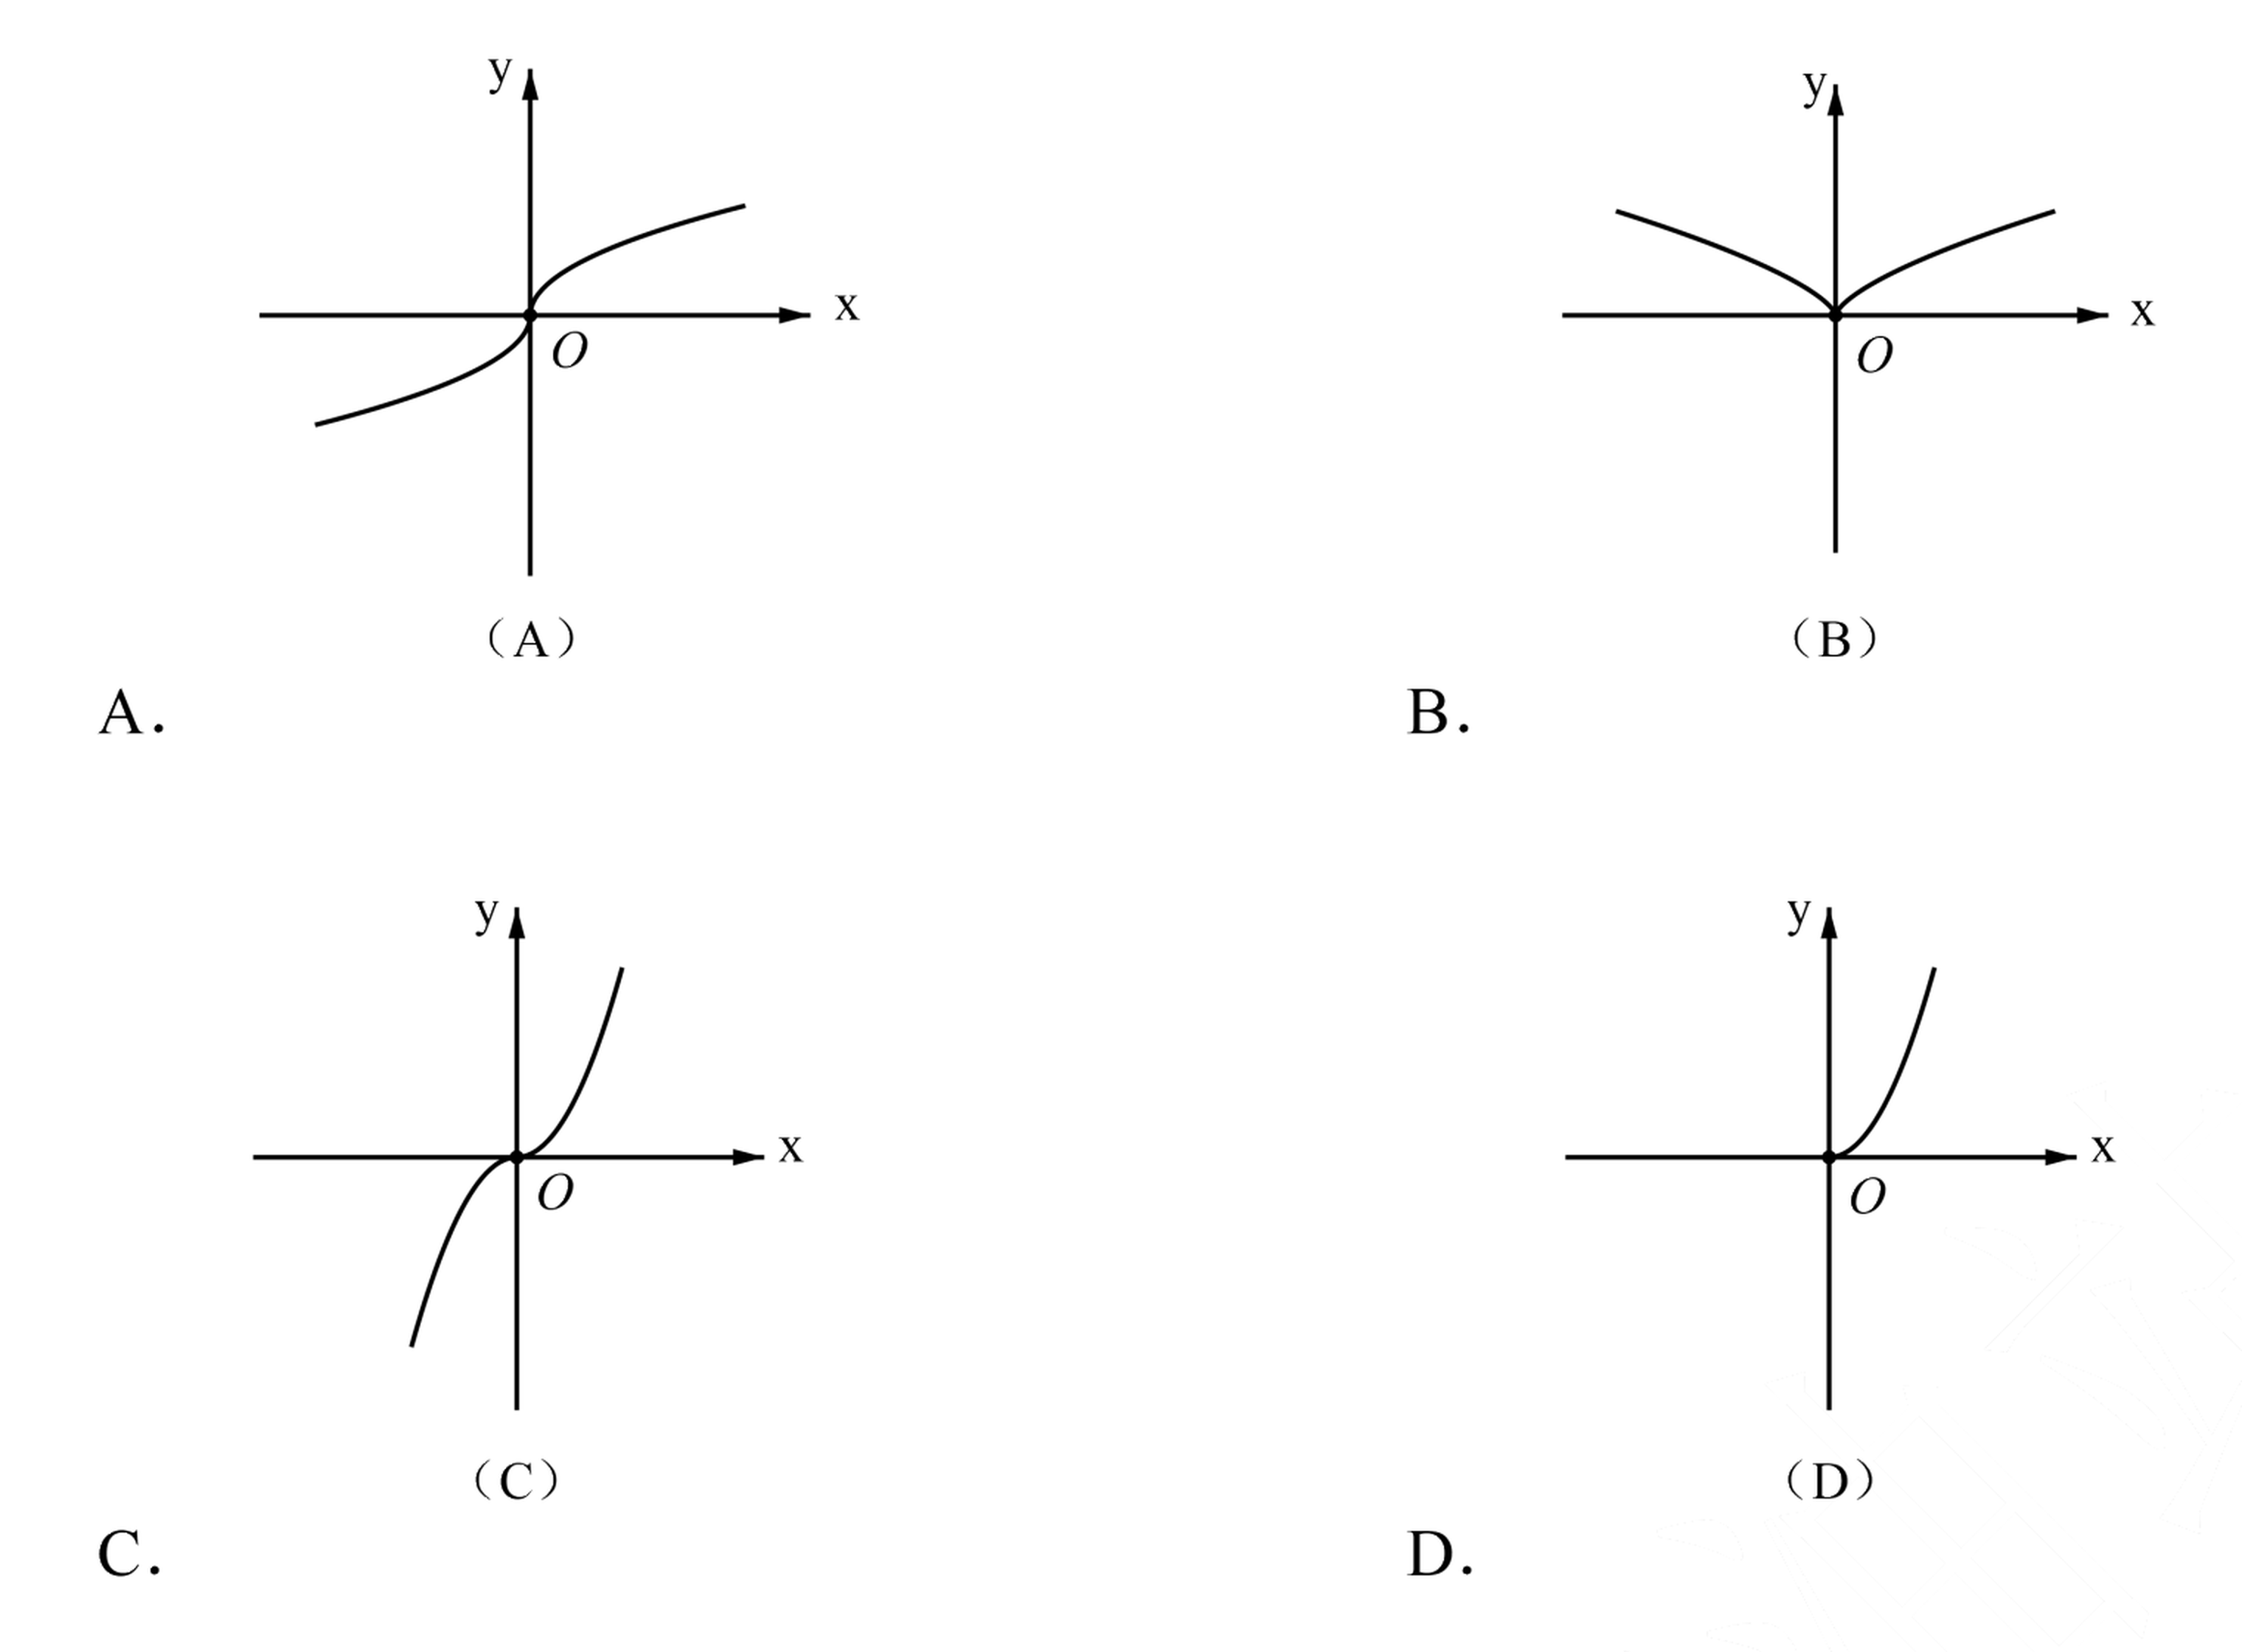
\includegraphics[width=0.80\textwidth]{figures/gao140_q14.png}
\end{center}

\ifanswer
\solbegin
\step{$f(x)=x^{\frac23}=\sqrt[3]{x^2}$ 是偶函数，且恒大于等于 $0$，故选 $B$.}
\solend
\fi

\item 设 $p$：关于 $x$ 的不等式 $x^2+ax+1>0$ 对 $x\in\R$ 恒成立，$q$：对数函数 $y=\log_{4-3a}x$ 在 $(0,+\infty)$ 上单调递减，那么 $p$ 是 $q$ 的\mbox{（\quad）}

\keepwithprev
A. 充分不必要条件\qquad B. 充要条件

C. 必要不充分条件\qquad D. 既不充分也不必要条件

\ifanswer
\solbegin
\step{$p\Leftrightarrow a^2-4<0\Leftrightarrow -2<a<2$. $q\Leftrightarrow 0<4-3a<1\Leftrightarrow 1<a<\dfrac43$.}
\step{由 $\left(1,\dfrac43\right)\subset(-2,2)$ 得 $q\Rightarrow p$；而 $a=0$ 时 $p$ 真、$q$ 假，}% 子集符号原卷印单线 $\subset$，照录
\step{故 $p$ 是 $q$ 的必要不充分条件，故选 $C$.}
\solend
\fi

\item “非空集合 $M$ 的元素都是集合 $P$ 的元素” 是假命题，现有下列命题：

(1) $M$ 的元素都不是 $P$ 的元素；(2) $M$ 中有不属于 $P$ 元素；% 原卷"不属于 P 元素"脱"的"字，照录

(3) $M$ 中有 $P$ 的元素；(4) $M$ 的元素不都是 $P$ 的元素，

其中真命题的个数是\mbox{（\quad）}

\keepwithprev
A. 1\qquad B. 2\qquad C. 3\qquad D. 4

\ifanswer
\solbegin
\step{由于 “非空集合 $M$ 的元素都是集合 $P$ 的元素” 是假命题，}
\step{得 “非空集合 $M$ 的元素至少有一个元素不属于集合 $P$” 是真命题.}
\step{则 (1) 不正确；(2) 正确；(3) $M$ 中不一定有 $P$ 的元素，例如 $M=\{a\}$，}
\step{则 $a\notin P$；(4) 正确.}
\step{综上，真命题只有 (2)(4). 故选 $B$.}
\solend
\fi

\end{enumerate}

\bigsec{三、解答题}

\begin{enumerate}
\setcounter{enumi}{16}

\item 设全集为 $\R$，集合 $A=\left\{x\mid\dfrac{2x}{x-1}\leqslant1\right\}$.

(1) 用区间表示集合 $A$；

(2) 若集合 $B=\{x\mid\lvert x+2\rvert+\lvert x-1\rvert=3\}$，求 $A\cup B$.

\ifanswer
\solbegin
\step{(1) 由 $\dfrac{2x}{x-1}\leqslant1\Leftrightarrow\dfrac{x+1}{x-1}\leqslant0$，故 $A=[-1,1)$，则 $\overline{A}=(-\infty,-1)\cup[1,+\infty)$；}
\step{(2) 由 $B=\{x\mid\lvert x+2\rvert+\lvert x-1\rvert=3\}=[-2,1]$，}
\step{结合上一问有 $A=[-1,1)$，所以 $A\cup B=B=[-2,1]$.}
\solend
\fi

\item (1) 已知指数函数 $y=a^x(a>0$ 且 $a\neq1)$ 在区间 $[-1,1]$ 上的最大值与最小值之和等于 $\dfrac52$，求实数 $a$ 的值.

(2) 已知幂函数 $y=x^{m^2+7m+10}(m\in\Z)$ 的图像关于 $y$ 轴对称，且在 $(0,+\infty)$ 上严格减. 若 $(a-1)^{m^2+7m+10}\geqslant(1+2a)^{m^2+7m+10}$. 求实数 $a$ 的取值范围.

\ifanswer
\solbegin
\step{(1) 指数函数 $y=a^x$ 在区间 $[-1,1]$ 上单调，所以 $a^1+a^{-1}=\dfrac52$，}
\step{所以 $a=2$ 或 $a=\dfrac12$；}
\step{(2) 由题意得 $m^2+7m+10<0$，所以 $-5<m<-2$，又因为 $m\in\Z$，}
\step{所以 $m=-4$ 或 $m=-3$，}
\step{当 $m=-4$ 时，$y=x^{m^2+7m+10}=x^{-2}$，为偶函数，}
\step{当 $m=-3$ 时，$y=x^{m^2+7m+10}=x^{-2}$，为偶函数，}
\step{所以 $m^2+7m+10=-2$，所以 $(a-1)^{-2}\geqslant(1+2a)^{-2}$，}
\step{所以 $\lvert a-1\rvert\leqslant\lvert 1+2a\rvert$，所以 $a\leqslant-2$ 或 $a\geqslant0$，所以 $a\in(-\infty,-2]\cup[0,+\infty)$.}
\solend
\fi

\item 设函数 $f(x)=ax^2+(1-a)x+a-2$ （$a\in\R$）.

(1) 若关于 $x$ 的不等式 $f(x)\leqslant0$ 的解集为 $\left[0,\dfrac12\right]$，求实数 $a$ 的值；

(2) 若 $a\geqslant0$，解关于 $x$ 的不等式：$f(x)<a-1$.

\ifanswer
\solbegin
\step{(1) 由解集得 $a>0$，且 $0$ 是方程 $f(x)=0$ 的根，故 $f(0)=a-2=0$，}
\step{得 $a=2$.}
\step{此时 $f(x)=2x^2-x=x(2x-1)$，$f(x)\leqslant0$ 的解集确为 $\left[0,\dfrac12\right]$.}
\step{(2) $f(x)<a-1\Leftrightarrow ax^2+(1-a)x-1<0\Leftrightarrow(x-1)(ax+1)<0$，}
\step{当 $a=0$ 时，$x-1<0$，解集为 $(-\infty,1)$.}
\step{当 $a>0$ 时，$-\dfrac1a<1$，解集为 $\left(-\dfrac1a,1\right)$.}
\solend
\fi

\item 为了保护环境，某单位采用新工艺，把二氧化碳转化为一种可利用的化工产品，已知该单位每月处理量最多不超过 $300$ 吨. 当月处理量为 $x$ 吨时，月处理成本为 $x^2-200x+40000(0<x\leqslant300)$ 元，且每处理一吨二氧化碳得到可利用的化工产品价值为 $300$ 元.

(1) 若要保证该单位每月不亏损，则每月处理量应控制在什么范围？

(2) 该单位每月处理量为多少吨时，才能使每吨的平均处理成本最低，最低为多少元？

\ifanswer
\solbegin
\step{(1) 由题意得 $S=300x-(x^2-200x+40000)$}
\step{$=-x^2+500x-40000(0<x\leqslant300)$，}
\step{令 $S\geqslant0$，即 $-x^2+500x-40000\geqslant0$，解得 $100\leqslant x\leqslant400$，}
\step{又 $0<x\leqslant300$，所以 $100\leqslant x\leqslant300$，}
\step{故要保证该单位每月不亏损，则每月处理量应控制在 $[100,300]$ 范围内；}
\step{(2) 每吨的平均出来成本为 $\dfrac yx=x+\dfrac{40000}x-200\geqslant2\sqrt{x\cdot\dfrac{40000}x}-200=200$，}% 原卷"平均出来成本"与题干"平均处理成本"措辞不一，照录
\step{当且仅当 $x=\dfrac{40000}x$，即 $x=200$ 时取等号，}
\step{所以该单位每月处理量为 $200$ 吨时，}
\step{才能使每吨的平均处理成本最低且最低为 $200$ 元.}
\solend
\fi

\item 已知函数 $y=f(x),x\in D$，若对于定义域 $D$ 内任意实数 $x,y$，不等式 $f(x)+f(y)\geqslant f(xy)$ 都成立，则称函数 $y=f(x)$ 是 $QB$ 函数，

(1) 判断函数 $f(x)=x+1$ 是否是 $QB$ 函数，并说明理由；

(2) 若函数 $g(x)=\ln(ax),x>0$ 是 $QB$ 函数，求实数 $a$ 的取值范围；

(3) 已知函数 $h(x)=a^x(a\in\R\text{ 且 }a>0)$，证明：“函数 $y=h(x)$ 是 $QB$ 函数” 的充要条件是 “ $a\in\{1\}$ ”.

\ifanswer
\solbegin
\step{(1) 不是，理由如下：因为 $f(x)=x+1$，}
\step{所以 $f(x)+f(y)\geqslant f(xy)\Leftrightarrow x+y\geqslant xy-1\Leftrightarrow(x-1)(y-1)\leqslant2$，}
\step{显然不恒成立，故不是 $QB$ 函数；}
\step{(2) 因为函数 $g(x)=\ln(ax),x>0$，则 $a>0$，}
\step{若函数 $g(x)$ 是 $QB$ 函数，则 $g(x)+g(y)\geqslant g(xy)$，}
\step{即 $\ln(ax)+\ln(ay)\geqslant\ln(axy)$，则 $\ln(a^2xy)\geqslant\ln(axy)$，得 $a^2xy\geqslant axy$，}
\step{且 $x>0,y>0$，得 $a^2\geqslant a$，解得 $a\geqslant1$ 或 $a\leqslant0$（舍去），}
\step{所以实数 $a$ 的取值范围为 $[1,+\infty)$.}
\step{(3) 若函数 $h(x)=a^x$ 是 $QB$ 函数，}
\step{当 $a>1$ 时，令 $x=y=\log_a\dfrac12$，则 $h(x)+h(y)=a^x+a^y=\dfrac12+\dfrac12=1$，}
\step{且 $h(xy)=a^{xy}=(a^x)^y=\left(\dfrac12\right)^{\log_a\frac12}=2^{\log_a2}$，}
\step{因为 $\log_a2>0$，所以 $h(xy)=2^{\log_a2}>1$，不满足 $h(x)+h(y)\geqslant h(xy)$，}
\step{不合题意；}
\step{当 $a=1$ 时，$h(x)+h(y)=a^x+a^y=1+1=2$，且 $h(xy)=a^{xy}=1$，}
\step{满足 $h(x)+h(y)\geqslant h(xy)$，符合题意；}
\step{当 $0<a<1$ 时，令 $x=\log_a2,y=2$，则 $h(x)+h(y)=a^x+a^y=2+a^2$，}
\step{且 $h(xy)=a^{xy}=(a^x)^y=2^2=4$，}
\step{因为 $0<a<1$，所以 $0<a^2<1$，得 $2<2+a^2<3$，}
\step{不满足 $h(x)+h(y)\geqslant h(xy)$，不合题意；}
\step{综上所述，$a\in\{1\}$，即充分性成立；}% 原卷"充分性/必要性"两标签与所证方向互换，照录
\step{若 $a\in\{1\}$，则 $h(x)+h(y)=a^x+a^y=1+1=2$，且 $h(xy)=a^{xy}=1$，}
\step{得 $h(x)+h(y)\geqslant h(xy)$，所以函数 $h(x)=a^x$ 是 $QB$ 函数，即必要性成立；}% 原卷"充分性/必要性"两标签与所证方向互换，照录
\step{综上所述，“函数 $y=h(x)$ 是 $QB$ 函数” 的充要条件是 “ $a\in\{1\}$ ”.}
\solend
\fi

\end{enumerate}

\end{document}
"
%
% ① 原始材料：微信公众号"魔都数学加油站"文章，连载"27学年高一140"，原文标题
% "27学年高一140——2026-2027年上海市甘泉外国语高一上期中"；
% 原文链接：https://mp.weixin.qq.com/s/eflgf2Ktk1LyT9x-k-ltLw。
% 正文为 9 张 PNG 页（01、02、03、05、06、07、08 为 4762x6735；04、09 为 2560x3620，
% 同一篇各页分辨率不同，逐页按各自分辨率裁图核对），题目下印有【答案】或【解析】，为讲评版。
% 题目、解析均据原图转录；卷面粉红色水印"魔都数学加油站"及公众号页脚未录入。
% 全卷 1 幅插图：第 14 题四幅坐标函数图象选项（04 页），取原卷截图去粉色水印、去色、
% LANCZOS 放大 2 倍，四幅选项按原卷 2x2 排布（含（A）（B）（C）（D）图注与 A./B./C./D.
% 选项字母）合并裁为一张；图前按惯例加 \needvspace 守卫。
%
% 卷首标题：原卷印作"2026-2027 年甘泉外国语高一上期中"（公众号标题中的"上海市"
% 卷面标题行没有，本稿照卷面），年份区间按全稿惯例排 en dash；原卷未印副标题，
% 本卷为期中卷、跨集合与常用逻辑用语／不等式／函数三章，按题目内容标为
% "集合与常用逻辑用语、不等式、函数"（与 125／126／128／129／131／132／133 同期中卷口径相同）：
% 集合与逻辑见 Q5、Q13、Q15、Q16、Q17，不等式见 Q3、Q10、Q11、Q19、Q20，
% 函数（指数／对数／幂函数及其图象、同构与 QB 函数）见 Q4、Q6、Q7、Q8、Q12、Q14、Q18、Q21。
%
% 题号体例：本卷共 19 题——一、填空题 3—12（10 题）、二、选择题 13—16（4 题）、
% 三、解答题 17—21（5 题）。三节分别 \setcounter{enumi}{2}／{12}／{16}。
% 原卷从第 3 题起、无第 1、2 题，本稿保留原题号。
%
% ② 与原卷的排版差异：
%   ① 原文从第 3 题起，本稿保留原题号；
%   ② 原卷每题下直接印【答案】或【解析】，本稿按全稿惯例置于答案版；第 5 题只印
%      【答案】、无【解析】，提 \ans{}；第 13、14、15、16 题答案均在【解析】末句
%      "故选 …"，题干括号内留空、不另提 \ans{}；其余各题印【解析】、无独立答案段；
%      全卷无"答案印在题干括号内且无解析"的一型；
%   ③ 原卷未印副标题，本稿按"知识模块"口径补出；
%   ④ 原卷填空横线按全稿惯例排为 \blankline[4.4em]；选择题括号排 \mbox{（\quad）}、
%      每个选项段前按惯例加 \keepwithprev（四幅图选项那一枚放在 \begin{center} 之前）；
%      解答题不留作答区、不加 \anspace（原卷为讲评版，与 129／131／132／133／136 同）；
%   ⑤ 原卷数集混排：斜体 $R$（Q9、Q12、Q15 等）与黑体／黑板粗体 $R$（Q15、Q17、
%      Q19、Q21）、粗体 $Z$（Q18），按全稿惯例统一改 \R／\Z；空集记号 \varnothing；
%      绝对值排 \lvert…\rvert，集合描述竖线排 \mid；不等号按全稿惯例排 \leqslant／\geqslant；
%      补集照原卷上划线排 \overline{A}；
%   ⑥ 子题标号 (1)(2)(3)(4) 原卷印半角括号，照录（与 131／132／133／134／136 同口径）；
%      括注原卷全角／半角混用，逐处照录：Q8"（结果用 a,b 表示）"、Q19"（a∈R）"、
%      Q21 (2)"（舍去）"印全角，Q18"$a^x(a>0$ 且 $a\neq1)$"、Q20"$40000(0<x\leqslant300)$"、
%      Q21 (3)"($a\in\R$ 且 $a>0$)"及 (0,+∞)、2(a>0) 等数学式内括注印半角；
%   ⑦ 数学式内半角逗号照录（如 Q8"$\lg2=a,10^b=3$"、Q11"$-2,3,4,\cdots,2027$"、
%      Q12"$x_1,x_2$"、Q19"$f(x)=ax^2+(1-a)x+a-2$"、Q21"$x>0,y>0$"）；
%      原卷行末西文句点照录（Q20 题干"300 吨. 当月处理量为 x 吨时"），行中全角逗号照录；
%   ⑧ 一幅插图：第 14 题四幅坐标函数图象选项合并裁为一张 \includegraphics
%      （题前 \needvspace{9cm}）。Q14 是"二、选择题"节内带大图块的第二题
%      （Q13 为节首题但无图），另在 \bigsec{二、选择题} 之前加 \needvspace{11cm}
%      连节标题一起量——守卫必须放在 \bigsec 之前，放标题之后会让"二、选择题"
%      孤立在页末（B 类，照 高一26／40／59／136 成例）；三版切页审计均"合计异常：无"；
%   ⑨ 跨页续印按题合并：Q9 题干在 01 页、解析续至 02 页；Q11 题干与解析前 3 行在 02 页、
%      后 2 行在 03 页；Q14 题干在 03 页末、四幅图与【解析】在 04 页；Q16 题干四条命题
%      在 04 页、选项与【解析】在 05 页；Q18 解析 (1) 首行在 05 页、其余 7 行在 06 页；
%      Q20 题干在 06 页末、"300 元."与两小问及【解析】在 07 页；Q21 解析跨 07—09 页
%      （末 3 行在 09 页）；本稿按题连排，不丢行；
%   ⑩ 题干中的中文弯引号按原卷照录，注释内一律 ASCII 引号；原卷"图像／图象"
%      两种写法混用，逐处照录（Q7、Q18 作"图像"，Q14 作"图象"）；
%   ⑪ 原卷无红色加粗标签（【解析】【答案】均黑色印刷），故本卷未用 \stepm。
%
% 判别式字形：全卷仅第 9 题【解析】"经验证得"cases 块出现两处判别式
%   "$\Delta=p^2-4q>0$"与"$\Delta'=q^2-4p>0$"，原卷两处均印等腰、偏高的
%   三角 $\Delta$（带撇的为 $\Delta'$），逐处放大核对并照录 \Delta、\Delta'；
%   全卷未出现扁等边三角 \triangle。
%
% 子集符号：第 15 题【解析】"由 (1,4/3)⊂(-2,2) 得 q⇒p"一处原卷印单线 $\subset$
%   （不带下划线），逐处放大核对、照录 \subset；全卷未出现带下划线的 \subseteq。
%
% 原卷存疑照录（均照录未改，正文对应处另有 % 注）：
%   第 16 题 (2) 命题"$M$ 中有不属于 $P$ 元素"中"不属于 $P$ 元素"脱"的"字，照录；
%   第 20 题题干 (2) 作"每吨的平均处理成本"、而【解析】(2) 作"每吨的平均出来成本"，
%      "出来"疑为"处理"之误，两处措辞照录不统一；
%   第 21 题 (3)【解析】"综上所述，$a\in\{1\}$，即充分性成立"与"即必要性成立"
%      两处标签与所证方向互换（按充要条件的通常口径），照录。
%
% 行数复核：一条 \step = 原卷解析的一个印刷行，cases 块作一个印刷行计。逐题数 \step
%   条数，合计 92 条（Q3：2；Q4：1；Q5：0；Q6：2；Q7：1；Q8：1；Q9：7；Q10：5；
%   Q11：5；Q12：4；Q13：6；Q14：1；Q15：3；Q16：5；Q17：3；Q18：8；Q19：6；
%   Q20：9；Q21：23），与原卷印刷行逐题相等。第 5 题只印【答案】、提 \ans{}，
%   不计入 \step 账；第 13、14、15、16 题答案在解析末句"故选 …"，括号内留空、
%   不另提 \ans{}；答案版【答案】/【解析】标记数 = 19（1 个 \ans + 18 个 \solbegin）
%   = 全卷题数。
%
\documentclass[a4paper,11pt]{article}
\usepackage{common}

\begin{document}

\examtitlest[3]{2026--2027 年甘泉外国语高一上期中}{集合与常用逻辑用语、不等式、函数}

\bigsec{一、填空题}

\begin{enumerate}
\setcounter{enumi}{2}

\item 不等式 $x^2-2x-3<0$ 的解集为\blankline[4.4em].

\ifanswer
\solbegin
\step{方程 $x^2-2x-3=0$ 的实数根是 $x_1=-1$，$x_2=3$；}
\step{所以不等式 $x^2-2x-3<0$ 的解集为 $\{x\mid -1<x<3\}$.}
\solend
\fi

\item 根式 $\sqrt{x\sqrt{x}}(x>0)$ 的指数幂形式为\blankline[4.4em].

\ifanswer
\solbegin
\step{$\sqrt{x\sqrt{x}}=\sqrt{x\cdot x^{\frac12}}=\sqrt{x^{\frac32}}=x^{\frac34}$.}
\solend
\fi

\item 陈述句 “ $x>1$ 或 $y>1$ ” 的否定形式是\blankline[4.4em].

\ifanswer
\ans{$x\leqslant1$ 且 $y\leqslant1$}
\fi

\item 若 $x<0$ 时，指数函数 $y=(a-1)^x$ 的值总大于 $1$，则实数 $a$ 的取值范围是\blankline[4.4em].

\ifanswer
\solbegin
\step{由题意得 $(a-1)^x>1$ 在 $(-\infty,0)$ 上恒成立，则 $0<a-1<1$，解得 $1<a<2$.}
\step{故实数 $a$ 的取值范围是 $(1,2)$.}
\solend
\fi

\item 若 $f(x)=\log_a(x-1)$，对任意 $a>0$ 且 $a\neq1$，函数 $y=f(x)$ 的图像必过定点\blankline[4.4em].

\ifanswer
\solbegin
\step{令 $x-1=1$，即 $x=2$，此时 $f(2)=0$，即函数图像过定点 $(2,0)$.}
\solend
\fi

\item 已知 $\lg 2=a,10^b=3$，则 $\log_6 2=$\blankline[4.4em]（结果用 $a,b$ 表示）.

\ifanswer
\solbegin
\step{由 $10^b=3$，得 $b=\lg 3$，则 $\log_6 2=\dfrac{\lg 2}{\lg 6}=\dfrac{\lg 2}{\lg 2+\lg 3}=\dfrac{a}{a+b}$.}
\solend
\fi

\item 已知 $p$、$q\in\R$，$x_1$、$x_2$ 是关于 $x$ 的方程 $x^2+px+q=0$ 的两实根，$x_1+1$、$x_2+1$ 是关于 $x$ 的方程 $x^2+qx+p=0$ 的两实根，则 $pq=$\blankline[4.4em].

\ifanswer
\solbegin
\step{因为 $x_1$、$x_2$ 是关于 $x$ 的方程 $x^2+px+q=0$ 的两实根，}
\step{由韦达定理得 $x_1+x_2=-p$，$x_1\cdot x_2=q$，}
\step{因为 $x_1+1$、$x_2+1$ 是关于 $x$ 的方程 $x^2+qx+p=0$ 的两实根，}
\step{由韦达定理得 $x_1+1+x_2+1=-q$，$(x_1+1)(x_2+1)=p$，}
\step{即 $x_1+x_2=-q-2$，$x_1+x_2+x_1x_2=p-1$，又 $x_1+x_2=-p$，$x_1\cdot x_2=q$，}
\step{所以 $\begin{cases}-p=-q-2\\-p+q=p-1\end{cases}$，解得 $\begin{cases}p=-1\\q=-3\end{cases}$，经验证得 $\begin{cases}\Delta=p^2-4q>0\\\Delta'=q^2-4p>0\end{cases}$，}% 判别式原卷印高三角 $\Delta$、$\Delta'$，照录
\step{则 $pq=3$.}
\solend
\fi

\item 对于 $x\in\R$，不等式 $\lvert 3-x\rvert+\lvert 1+x\rvert\geqslant a^2-3a$ 恒成立，则实数 $a$ 的取值范围是\blankline[4.4em].

\ifanswer
\solbegin
\step{对于 $x\in\R$，不等式 $\lvert 3-x\rvert+\lvert 1+x\rvert\geqslant a^2-3a$ 恒成立，}
\step{即 $\lvert 3-x\rvert+\lvert 1+x\rvert$ 的最小值大于或等于 $a^2-3a$，}
\step{$\lvert 3-x\rvert+\lvert 1+x\rvert$ 表示数轴上的 $x$ 对应点到 $3$ 和 $-1$ 对应点的距离之和，}
\step{它的最小值为 $4$，故 $4\geqslant a^2-3a$，即 $a^2-3a-4\leqslant0$，解得 $-1\leqslant a\leqslant4$，}
\step{故实数 $a$ 的取值范围是 $[-1,4]$.}
\solend
\fi

\item 已知同时满足不等式 $x^2-x-2>0$ 和 $2x^2+(5+2a)x+5a<0$ 的 $x$ 的整数值只有 $2026$ 个，则实数 $a$ 的取值范围是\blankline[4.4em].

\ifanswer
\solbegin
\step{整数 $x$ 须满足 $x\leqslant-2$ 或 $x\geqslant3$，且 $(2x+5)(x+a)<0$.}
\step{当 $a<\dfrac52$ 时，需使整数解恰为 $-2,3,4,\cdots,2027$，即 $2027<-a\leqslant2028$.}
\step{当 $a>\dfrac52$ 时，需使整数解恰为 $-2028,-2027,\cdots,-3$，即 $2028<a\leqslant2029$；}
\step{$a=\dfrac52$ 时无解.}
\step{故 $a\in[-2028,-2027)\cup(2028,2029]$.}
\solend
\fi

\item 同构式通俗讲是结构相同的表达式，如：$f(x)=x+e^x$，$f(\ln x)=\ln x+e^{\ln x}=\ln x+x$，称 $x+e^x$ 与 $\ln x+x$ 为同构式. 已知实数 $x_1,x_2$ 满足 $e^{x_1}+x_1=8,\ln\sqrt[5]{5x_2+3}+x_2=1$，则 $x_1+5x_2=$\blankline[4.4em].

\ifanswer
\solbegin
\step{函数 $f(x)=x+e^x$ 在 $\R$ 上严格增，且 $f(x_1)=x_1+e^{x_1}=8$，}
\step{由 $\ln\sqrt[5]{5x_2+3}+x_2=1$，得 $\ln(5x_2+3)+5x_2=5$，则 $\ln(5x_2+3)+5x_2+3=8$，}
\step{即 $f(\ln(5x_2+3))=8$，因此 $f(\ln(5x_2+3))=8=f(x_1)$，则 $x_1=\ln(5x_2+3)$，}
\step{所以 $x_1+5x_2=\ln(5x_2+3)+5x_2=5$.}
\solend
\fi

\end{enumerate}

% 第 14 题四幅图是"二、选择题"节内的大图块；守卫须放在 \bigsec 之前连节标题一起量，
% 否则"二、选择题"会孤立在页末（B 类，照 高一26／40／59／136 成例）
\needvspace{11cm}
\bigsec{二、选择题}

\begin{enumerate}
\setcounter{enumi}{12}

\item 设 $a$、$b$ 为实数，则 “ $a>b>0$ ” 的一个充分非必要条件是\mbox{（\quad）}

\keepwithprev
A. $\sqrt{a-1}>\sqrt{b-1}$\qquad B. $a^2>b^2$

C. $\dfrac1b>\dfrac1a$\qquad D. $a-b>b-a$

\ifanswer
\solbegin
\step{由 $\sqrt{a-1}>\sqrt{b-1}$ 得 $a>b\geqslant1$，故 $a>b>0$，反之不成立，满足题意；}
\step{由 $a^2>b^2$，则 $\lvert a\rvert>\lvert b\rvert$，推不出 $a>b>0$，反向可推出，不满足；}
\step{由 $\dfrac1b>\dfrac1a$，则 $a>b>0$ 或 $b>0>a$ 或 $0>a>b$，推不出 $a>b>0$，}
\step{反向可推出，不满足；}
\step{由 $a-b>b-a$，则 $a>b$，推不出 $a>b>0$，反向可推出，不满足；}
\step{故选 $A$.}
\solend
\fi

% 第 14 题四幅坐标函数图象选项是一整块，守卫放在 \item 之前
\needvspace{9cm}
\item 幂函数 $f(x)=x^{\frac23}$ 的图象大致为\mbox{（\quad）}

\keepwithprev
\begin{center}
% 四幅坐标函数图象选项取原卷 04 页截图去粉色水印、去色，按原卷 2x2 排布合并为一张
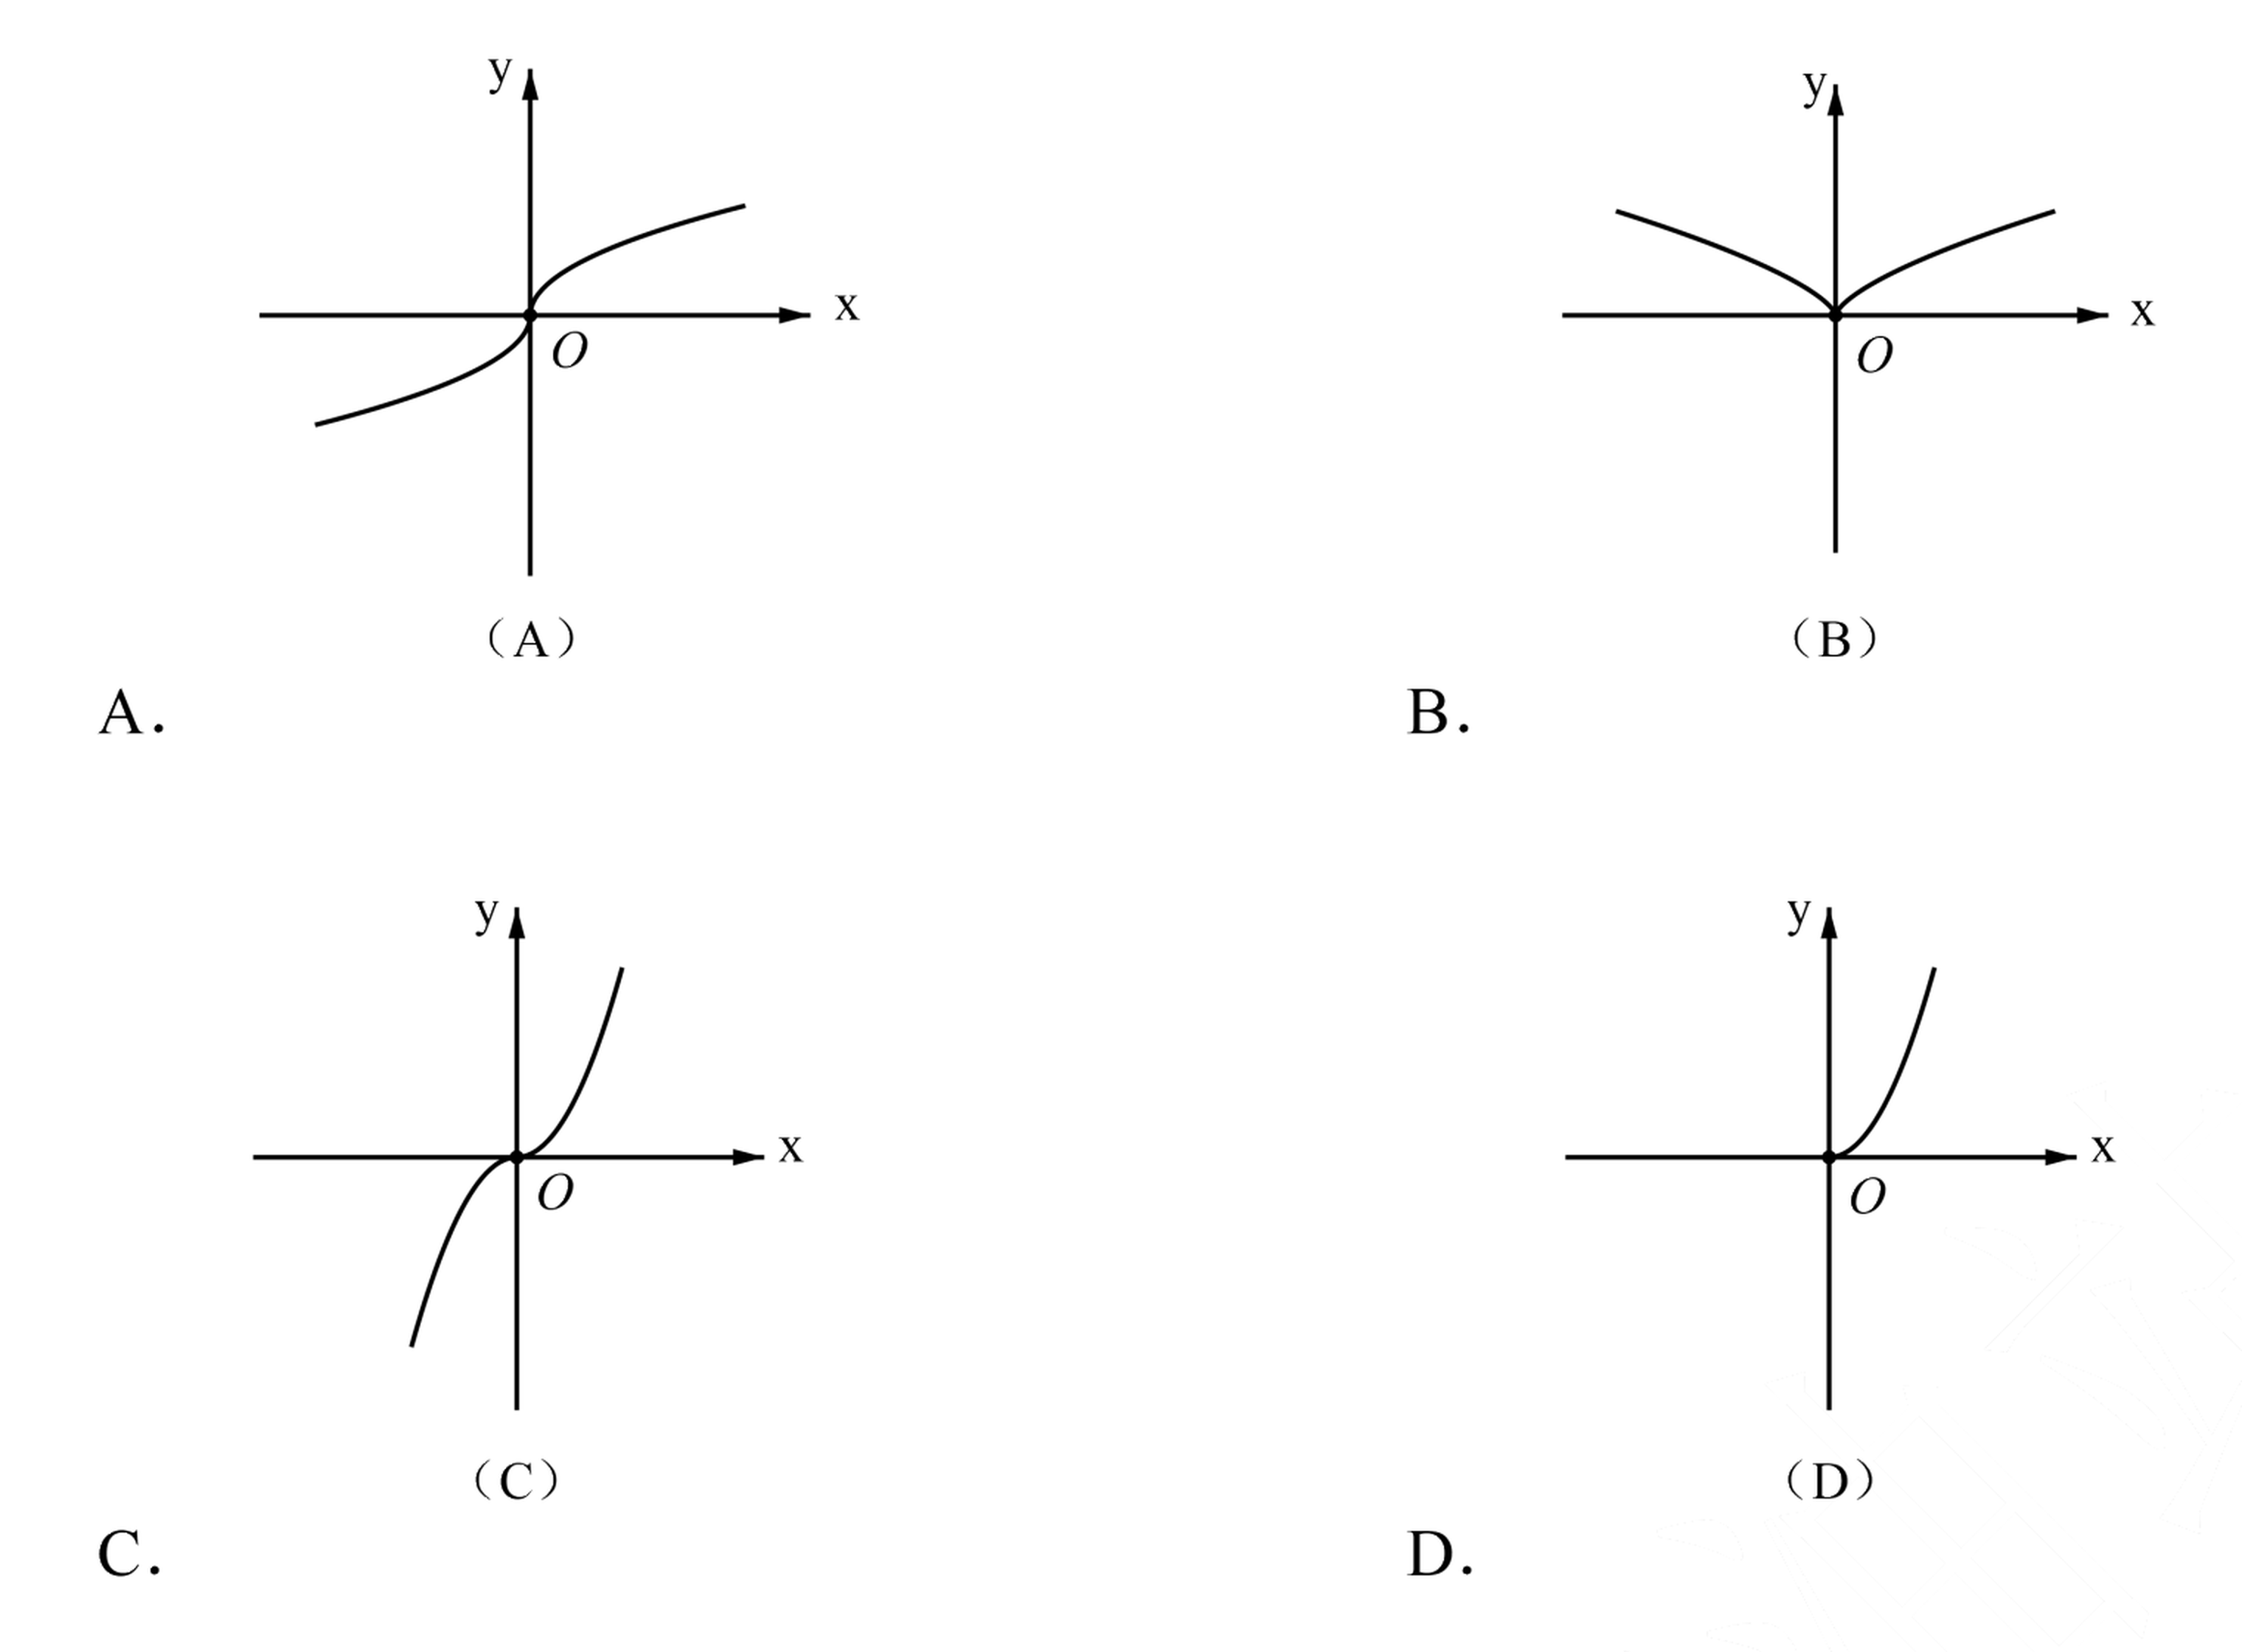
\includegraphics[width=0.80\textwidth]{figures/gao140_q14.png}
\end{center}

\ifanswer
\solbegin
\step{$f(x)=x^{\frac23}=\sqrt[3]{x^2}$ 是偶函数，且恒大于等于 $0$，故选 $B$.}
\solend
\fi

\item 设 $p$：关于 $x$ 的不等式 $x^2+ax+1>0$ 对 $x\in\R$ 恒成立，$q$：对数函数 $y=\log_{4-3a}x$ 在 $(0,+\infty)$ 上单调递减，那么 $p$ 是 $q$ 的\mbox{（\quad）}

\keepwithprev
A. 充分不必要条件\qquad B. 充要条件

C. 必要不充分条件\qquad D. 既不充分也不必要条件

\ifanswer
\solbegin
\step{$p\Leftrightarrow a^2-4<0\Leftrightarrow -2<a<2$. $q\Leftrightarrow 0<4-3a<1\Leftrightarrow 1<a<\dfrac43$.}
\step{由 $\left(1,\dfrac43\right)\subset(-2,2)$ 得 $q\Rightarrow p$；而 $a=0$ 时 $p$ 真、$q$ 假，}% 子集符号原卷印单线 $\subset$，照录
\step{故 $p$ 是 $q$ 的必要不充分条件，故选 $C$.}
\solend
\fi

\item “非空集合 $M$ 的元素都是集合 $P$ 的元素” 是假命题，现有下列命题：

(1) $M$ 的元素都不是 $P$ 的元素；(2) $M$ 中有不属于 $P$ 元素；% 原卷"不属于 P 元素"脱"的"字，照录

(3) $M$ 中有 $P$ 的元素；(4) $M$ 的元素不都是 $P$ 的元素，

其中真命题的个数是\mbox{（\quad）}

\keepwithprev
A. 1\qquad B. 2\qquad C. 3\qquad D. 4

\ifanswer
\solbegin
\step{由于 “非空集合 $M$ 的元素都是集合 $P$ 的元素” 是假命题，}
\step{得 “非空集合 $M$ 的元素至少有一个元素不属于集合 $P$” 是真命题.}
\step{则 (1) 不正确；(2) 正确；(3) $M$ 中不一定有 $P$ 的元素，例如 $M=\{a\}$，}
\step{则 $a\notin P$；(4) 正确.}
\step{综上，真命题只有 (2)(4). 故选 $B$.}
\solend
\fi

\end{enumerate}

\bigsec{三、解答题}

\begin{enumerate}
\setcounter{enumi}{16}

\item 设全集为 $\R$，集合 $A=\left\{x\mid\dfrac{2x}{x-1}\leqslant1\right\}$.

(1) 用区间表示集合 $A$；

(2) 若集合 $B=\{x\mid\lvert x+2\rvert+\lvert x-1\rvert=3\}$，求 $A\cup B$.

\ifanswer
\solbegin
\step{(1) 由 $\dfrac{2x}{x-1}\leqslant1\Leftrightarrow\dfrac{x+1}{x-1}\leqslant0$，故 $A=[-1,1)$，则 $\overline{A}=(-\infty,-1)\cup[1,+\infty)$；}
\step{(2) 由 $B=\{x\mid\lvert x+2\rvert+\lvert x-1\rvert=3\}=[-2,1]$，}
\step{结合上一问有 $A=[-1,1)$，所以 $A\cup B=B=[-2,1]$.}
\solend
\fi

\item (1) 已知指数函数 $y=a^x(a>0$ 且 $a\neq1)$ 在区间 $[-1,1]$ 上的最大值与最小值之和等于 $\dfrac52$，求实数 $a$ 的值.

(2) 已知幂函数 $y=x^{m^2+7m+10}(m\in\Z)$ 的图像关于 $y$ 轴对称，且在 $(0,+\infty)$ 上严格减. 若 $(a-1)^{m^2+7m+10}\geqslant(1+2a)^{m^2+7m+10}$. 求实数 $a$ 的取值范围.

\ifanswer
\solbegin
\step{(1) 指数函数 $y=a^x$ 在区间 $[-1,1]$ 上单调，所以 $a^1+a^{-1}=\dfrac52$，}
\step{所以 $a=2$ 或 $a=\dfrac12$；}
\step{(2) 由题意得 $m^2+7m+10<0$，所以 $-5<m<-2$，又因为 $m\in\Z$，}
\step{所以 $m=-4$ 或 $m=-3$，}
\step{当 $m=-4$ 时，$y=x^{m^2+7m+10}=x^{-2}$，为偶函数，}
\step{当 $m=-3$ 时，$y=x^{m^2+7m+10}=x^{-2}$，为偶函数，}
\step{所以 $m^2+7m+10=-2$，所以 $(a-1)^{-2}\geqslant(1+2a)^{-2}$，}
\step{所以 $\lvert a-1\rvert\leqslant\lvert 1+2a\rvert$，所以 $a\leqslant-2$ 或 $a\geqslant0$，所以 $a\in(-\infty,-2]\cup[0,+\infty)$.}
\solend
\fi

\item 设函数 $f(x)=ax^2+(1-a)x+a-2$ （$a\in\R$）.

(1) 若关于 $x$ 的不等式 $f(x)\leqslant0$ 的解集为 $\left[0,\dfrac12\right]$，求实数 $a$ 的值；

(2) 若 $a\geqslant0$，解关于 $x$ 的不等式：$f(x)<a-1$.

\ifanswer
\solbegin
\step{(1) 由解集得 $a>0$，且 $0$ 是方程 $f(x)=0$ 的根，故 $f(0)=a-2=0$，}
\step{得 $a=2$.}
\step{此时 $f(x)=2x^2-x=x(2x-1)$，$f(x)\leqslant0$ 的解集确为 $\left[0,\dfrac12\right]$.}
\step{(2) $f(x)<a-1\Leftrightarrow ax^2+(1-a)x-1<0\Leftrightarrow(x-1)(ax+1)<0$，}
\step{当 $a=0$ 时，$x-1<0$，解集为 $(-\infty,1)$.}
\step{当 $a>0$ 时，$-\dfrac1a<1$，解集为 $\left(-\dfrac1a,1\right)$.}
\solend
\fi

\item 为了保护环境，某单位采用新工艺，把二氧化碳转化为一种可利用的化工产品，已知该单位每月处理量最多不超过 $300$ 吨. 当月处理量为 $x$ 吨时，月处理成本为 $x^2-200x+40000(0<x\leqslant300)$ 元，且每处理一吨二氧化碳得到可利用的化工产品价值为 $300$ 元.

(1) 若要保证该单位每月不亏损，则每月处理量应控制在什么范围？

(2) 该单位每月处理量为多少吨时，才能使每吨的平均处理成本最低，最低为多少元？

\ifanswer
\solbegin
\step{(1) 由题意得 $S=300x-(x^2-200x+40000)$}
\step{$=-x^2+500x-40000(0<x\leqslant300)$，}
\step{令 $S\geqslant0$，即 $-x^2+500x-40000\geqslant0$，解得 $100\leqslant x\leqslant400$，}
\step{又 $0<x\leqslant300$，所以 $100\leqslant x\leqslant300$，}
\step{故要保证该单位每月不亏损，则每月处理量应控制在 $[100,300]$ 范围内；}
\step{(2) 每吨的平均出来成本为 $\dfrac yx=x+\dfrac{40000}x-200\geqslant2\sqrt{x\cdot\dfrac{40000}x}-200=200$，}% 原卷"平均出来成本"与题干"平均处理成本"措辞不一，照录
\step{当且仅当 $x=\dfrac{40000}x$，即 $x=200$ 时取等号，}
\step{所以该单位每月处理量为 $200$ 吨时，}
\step{才能使每吨的平均处理成本最低且最低为 $200$ 元.}
\solend
\fi

\item 已知函数 $y=f(x),x\in D$，若对于定义域 $D$ 内任意实数 $x,y$，不等式 $f(x)+f(y)\geqslant f(xy)$ 都成立，则称函数 $y=f(x)$ 是 $QB$ 函数，

(1) 判断函数 $f(x)=x+1$ 是否是 $QB$ 函数，并说明理由；

(2) 若函数 $g(x)=\ln(ax),x>0$ 是 $QB$ 函数，求实数 $a$ 的取值范围；

(3) 已知函数 $h(x)=a^x(a\in\R\text{ 且 }a>0)$，证明：“函数 $y=h(x)$ 是 $QB$ 函数” 的充要条件是 “ $a\in\{1\}$ ”.

\ifanswer
\solbegin
\step{(1) 不是，理由如下：因为 $f(x)=x+1$，}
\step{所以 $f(x)+f(y)\geqslant f(xy)\Leftrightarrow x+y\geqslant xy-1\Leftrightarrow(x-1)(y-1)\leqslant2$，}
\step{显然不恒成立，故不是 $QB$ 函数；}
\step{(2) 因为函数 $g(x)=\ln(ax),x>0$，则 $a>0$，}
\step{若函数 $g(x)$ 是 $QB$ 函数，则 $g(x)+g(y)\geqslant g(xy)$，}
\step{即 $\ln(ax)+\ln(ay)\geqslant\ln(axy)$，则 $\ln(a^2xy)\geqslant\ln(axy)$，得 $a^2xy\geqslant axy$，}
\step{且 $x>0,y>0$，得 $a^2\geqslant a$，解得 $a\geqslant1$ 或 $a\leqslant0$（舍去），}
\step{所以实数 $a$ 的取值范围为 $[1,+\infty)$.}
\step{(3) 若函数 $h(x)=a^x$ 是 $QB$ 函数，}
\step{当 $a>1$ 时，令 $x=y=\log_a\dfrac12$，则 $h(x)+h(y)=a^x+a^y=\dfrac12+\dfrac12=1$，}
\step{且 $h(xy)=a^{xy}=(a^x)^y=\left(\dfrac12\right)^{\log_a\frac12}=2^{\log_a2}$，}
\step{因为 $\log_a2>0$，所以 $h(xy)=2^{\log_a2}>1$，不满足 $h(x)+h(y)\geqslant h(xy)$，}
\step{不合题意；}
\step{当 $a=1$ 时，$h(x)+h(y)=a^x+a^y=1+1=2$，且 $h(xy)=a^{xy}=1$，}
\step{满足 $h(x)+h(y)\geqslant h(xy)$，符合题意；}
\step{当 $0<a<1$ 时，令 $x=\log_a2,y=2$，则 $h(x)+h(y)=a^x+a^y=2+a^2$，}
\step{且 $h(xy)=a^{xy}=(a^x)^y=2^2=4$，}
\step{因为 $0<a<1$，所以 $0<a^2<1$，得 $2<2+a^2<3$，}
\step{不满足 $h(x)+h(y)\geqslant h(xy)$，不合题意；}
\step{综上所述，$a\in\{1\}$，即充分性成立；}% 原卷"充分性/必要性"两标签与所证方向互换，照录
\step{若 $a\in\{1\}$，则 $h(x)+h(y)=a^x+a^y=1+1=2$，且 $h(xy)=a^{xy}=1$，}
\step{得 $h(x)+h(y)\geqslant h(xy)$，所以函数 $h(x)=a^x$ 是 $QB$ 函数，即必要性成立；}% 原卷"充分性/必要性"两标签与所证方向互换，照录
\step{综上所述，“函数 $y=h(x)$ 是 $QB$ 函数” 的充要条件是 “ $a\in\{1\}$ ”.}
\solend
\fi

\end{enumerate}

\end{document}
"
%
% ① 原始材料：微信公众号"魔都数学加油站"文章，连载"27学年高一140"，原文标题
% "27学年高一140——2026-2027年上海市甘泉外国语高一上期中"；
% 原文链接：https://mp.weixin.qq.com/s/eflgf2Ktk1LyT9x-k-ltLw。
% 正文为 9 张 PNG 页（01、02、03、05、06、07、08 为 4762x6735；04、09 为 2560x3620，
% 同一篇各页分辨率不同，逐页按各自分辨率裁图核对），题目下印有【答案】或【解析】，为讲评版。
% 题目、解析均据原图转录；卷面粉红色水印"魔都数学加油站"及公众号页脚未录入。
% 全卷 1 幅插图：第 14 题四幅坐标函数图象选项（04 页），取原卷截图去粉色水印、去色、
% LANCZOS 放大 2 倍，四幅选项按原卷 2x2 排布（含（A）（B）（C）（D）图注与 A./B./C./D.
% 选项字母）合并裁为一张；图前按惯例加 \needvspace 守卫。
%
% 卷首标题：原卷印作"2026-2027 年甘泉外国语高一上期中"（公众号标题中的"上海市"
% 卷面标题行没有，本稿照卷面），年份区间按全稿惯例排 en dash；原卷未印副标题，
% 本卷为期中卷、跨集合与常用逻辑用语／不等式／函数三章，按题目内容标为
% "集合与常用逻辑用语、不等式、函数"（与 125／126／128／129／131／132／133 同期中卷口径相同）：
% 集合与逻辑见 Q5、Q13、Q15、Q16、Q17，不等式见 Q3、Q10、Q11、Q19、Q20，
% 函数（指数／对数／幂函数及其图象、同构与 QB 函数）见 Q4、Q6、Q7、Q8、Q12、Q14、Q18、Q21。
%
% 题号体例：本卷共 19 题——一、填空题 3—12（10 题）、二、选择题 13—16（4 题）、
% 三、解答题 17—21（5 题）。三节分别 \setcounter{enumi}{2}／{12}／{16}。
% 原卷从第 3 题起、无第 1、2 题，本稿保留原题号。
%
% ② 与原卷的排版差异：
%   ① 原文从第 3 题起，本稿保留原题号；
%   ② 原卷每题下直接印【答案】或【解析】，本稿按全稿惯例置于答案版；第 5 题只印
%      【答案】、无【解析】，提 \ans{}；第 13、14、15、16 题答案均在【解析】末句
%      "故选 …"，题干括号内留空、不另提 \ans{}；其余各题印【解析】、无独立答案段；
%      全卷无"答案印在题干括号内且无解析"的一型；
%   ③ 原卷未印副标题，本稿按"知识模块"口径补出；
%   ④ 原卷填空横线按全稿惯例排为 \blankline[4.4em]；选择题括号排 \mbox{（\quad）}、
%      每个选项段前按惯例加 \keepwithprev（四幅图选项那一枚放在 \begin{center} 之前）；
%      解答题不留作答区、不加 \anspace（原卷为讲评版，与 129／131／132／133／136 同）；
%   ⑤ 原卷数集混排：斜体 $R$（Q9、Q12、Q15 等）与黑体／黑板粗体 $R$（Q15、Q17、
%      Q19、Q21）、粗体 $Z$（Q18），按全稿惯例统一改 \R／\Z；空集记号 \varnothing；
%      绝对值排 \lvert…\rvert，集合描述竖线排 \mid；不等号按全稿惯例排 \leqslant／\geqslant；
%      补集照原卷上划线排 \overline{A}；
%   ⑥ 子题标号 (1)(2)(3)(4) 原卷印半角括号，照录（与 131／132／133／134／136 同口径）；
%      括注原卷全角／半角混用，逐处照录：Q8"（结果用 a,b 表示）"、Q19"（a∈R）"、
%      Q21 (2)"（舍去）"印全角，Q18"$a^x(a>0$ 且 $a\neq1)$"、Q20"$40000(0<x\leqslant300)$"、
%      Q21 (3)"($a\in\R$ 且 $a>0$)"及 (0,+∞)、2(a>0) 等数学式内括注印半角；
%   ⑦ 数学式内半角逗号照录（如 Q8"$\lg2=a,10^b=3$"、Q11"$-2,3,4,\cdots,2027$"、
%      Q12"$x_1,x_2$"、Q19"$f(x)=ax^2+(1-a)x+a-2$"、Q21"$x>0,y>0$"）；
%      原卷行末西文句点照录（Q20 题干"300 吨. 当月处理量为 x 吨时"），行中全角逗号照录；
%   ⑧ 一幅插图：第 14 题四幅坐标函数图象选项合并裁为一张 \includegraphics
%      （题前 \needvspace{9cm}）。Q14 是"二、选择题"节内带大图块的第二题
%      （Q13 为节首题但无图），另在 \bigsec{二、选择题} 之前加 \needvspace{11cm}
%      连节标题一起量——守卫必须放在 \bigsec 之前，放标题之后会让"二、选择题"
%      孤立在页末（B 类，照 高一26／40／59／136 成例）；三版切页审计均"合计异常：无"；
%   ⑨ 跨页续印按题合并：Q9 题干在 01 页、解析续至 02 页；Q11 题干与解析前 3 行在 02 页、
%      后 2 行在 03 页；Q14 题干在 03 页末、四幅图与【解析】在 04 页；Q16 题干四条命题
%      在 04 页、选项与【解析】在 05 页；Q18 解析 (1) 首行在 05 页、其余 7 行在 06 页；
%      Q20 题干在 06 页末、"300 元."与两小问及【解析】在 07 页；Q21 解析跨 07—09 页
%      （末 3 行在 09 页）；本稿按题连排，不丢行；
%   ⑩ 题干中的中文弯引号按原卷照录，注释内一律 ASCII 引号；原卷"图像／图象"
%      两种写法混用，逐处照录（Q7、Q18 作"图像"，Q14 作"图象"）；
%   ⑪ 原卷无红色加粗标签（【解析】【答案】均黑色印刷），故本卷未用 \stepm。
%
% 判别式字形：全卷仅第 9 题【解析】"经验证得"cases 块出现两处判别式
%   "$\Delta=p^2-4q>0$"与"$\Delta'=q^2-4p>0$"，原卷两处均印等腰、偏高的
%   三角 $\Delta$（带撇的为 $\Delta'$），逐处放大核对并照录 \Delta、\Delta'；
%   全卷未出现扁等边三角 \triangle。
%
% 子集符号：第 15 题【解析】"由 (1,4/3)⊂(-2,2) 得 q⇒p"一处原卷印单线 $\subset$
%   （不带下划线），逐处放大核对、照录 \subset；全卷未出现带下划线的 \subseteq。
%
% 原卷存疑照录（均照录未改，正文对应处另有 % 注）：
%   第 16 题 (2) 命题"$M$ 中有不属于 $P$ 元素"中"不属于 $P$ 元素"脱"的"字，照录；
%   第 20 题题干 (2) 作"每吨的平均处理成本"、而【解析】(2) 作"每吨的平均出来成本"，
%      "出来"疑为"处理"之误，两处措辞照录不统一；
%   第 21 题 (3)【解析】"综上所述，$a\in\{1\}$，即充分性成立"与"即必要性成立"
%      两处标签与所证方向互换（按充要条件的通常口径），照录。
%
% 行数复核：一条 \step = 原卷解析的一个印刷行，cases 块作一个印刷行计。逐题数 \step
%   条数，合计 92 条（Q3：2；Q4：1；Q5：0；Q6：2；Q7：1；Q8：1；Q9：7；Q10：5；
%   Q11：5；Q12：4；Q13：6；Q14：1；Q15：3；Q16：5；Q17：3；Q18：8；Q19：6；
%   Q20：9；Q21：23），与原卷印刷行逐题相等。第 5 题只印【答案】、提 \ans{}，
%   不计入 \step 账；第 13、14、15、16 题答案在解析末句"故选 …"，括号内留空、
%   不另提 \ans{}；答案版【答案】/【解析】标记数 = 19（1 个 \ans + 18 个 \solbegin）
%   = 全卷题数。
%
\documentclass[a4paper,11pt]{article}
\usepackage{common}

\begin{document}

\examtitlest[3]{2026--2027 年甘泉外国语高一上期中}{集合与常用逻辑用语、不等式、函数}

\bigsec{一、填空题}

\begin{enumerate}
\setcounter{enumi}{2}

\item 不等式 $x^2-2x-3<0$ 的解集为\blankline[4.4em].

\ifanswer
\solbegin
\step{方程 $x^2-2x-3=0$ 的实数根是 $x_1=-1$，$x_2=3$；}
\step{所以不等式 $x^2-2x-3<0$ 的解集为 $\{x\mid -1<x<3\}$.}
\solend
\fi

\item 根式 $\sqrt{x\sqrt{x}}(x>0)$ 的指数幂形式为\blankline[4.4em].

\ifanswer
\solbegin
\step{$\sqrt{x\sqrt{x}}=\sqrt{x\cdot x^{\frac12}}=\sqrt{x^{\frac32}}=x^{\frac34}$.}
\solend
\fi

\item 陈述句 “ $x>1$ 或 $y>1$ ” 的否定形式是\blankline[4.4em].

\ifanswer
\ans{$x\leqslant1$ 且 $y\leqslant1$}
\fi

\item 若 $x<0$ 时，指数函数 $y=(a-1)^x$ 的值总大于 $1$，则实数 $a$ 的取值范围是\blankline[4.4em].

\ifanswer
\solbegin
\step{由题意得 $(a-1)^x>1$ 在 $(-\infty,0)$ 上恒成立，则 $0<a-1<1$，解得 $1<a<2$.}
\step{故实数 $a$ 的取值范围是 $(1,2)$.}
\solend
\fi

\item 若 $f(x)=\log_a(x-1)$，对任意 $a>0$ 且 $a\neq1$，函数 $y=f(x)$ 的图像必过定点\blankline[4.4em].

\ifanswer
\solbegin
\step{令 $x-1=1$，即 $x=2$，此时 $f(2)=0$，即函数图像过定点 $(2,0)$.}
\solend
\fi

\item 已知 $\lg 2=a,10^b=3$，则 $\log_6 2=$\blankline[4.4em]（结果用 $a,b$ 表示）.

\ifanswer
\solbegin
\step{由 $10^b=3$，得 $b=\lg 3$，则 $\log_6 2=\dfrac{\lg 2}{\lg 6}=\dfrac{\lg 2}{\lg 2+\lg 3}=\dfrac{a}{a+b}$.}
\solend
\fi

\item 已知 $p$、$q\in\R$，$x_1$、$x_2$ 是关于 $x$ 的方程 $x^2+px+q=0$ 的两实根，$x_1+1$、$x_2+1$ 是关于 $x$ 的方程 $x^2+qx+p=0$ 的两实根，则 $pq=$\blankline[4.4em].

\ifanswer
\solbegin
\step{因为 $x_1$、$x_2$ 是关于 $x$ 的方程 $x^2+px+q=0$ 的两实根，}
\step{由韦达定理得 $x_1+x_2=-p$，$x_1\cdot x_2=q$，}
\step{因为 $x_1+1$、$x_2+1$ 是关于 $x$ 的方程 $x^2+qx+p=0$ 的两实根，}
\step{由韦达定理得 $x_1+1+x_2+1=-q$，$(x_1+1)(x_2+1)=p$，}
\step{即 $x_1+x_2=-q-2$，$x_1+x_2+x_1x_2=p-1$，又 $x_1+x_2=-p$，$x_1\cdot x_2=q$，}
\step{所以 $\begin{cases}-p=-q-2\\-p+q=p-1\end{cases}$，解得 $\begin{cases}p=-1\\q=-3\end{cases}$，经验证得 $\begin{cases}\Delta=p^2-4q>0\\\Delta'=q^2-4p>0\end{cases}$，}% 判别式原卷印高三角 $\Delta$、$\Delta'$，照录
\step{则 $pq=3$.}
\solend
\fi

\item 对于 $x\in\R$，不等式 $\lvert 3-x\rvert+\lvert 1+x\rvert\geqslant a^2-3a$ 恒成立，则实数 $a$ 的取值范围是\blankline[4.4em].

\ifanswer
\solbegin
\step{对于 $x\in\R$，不等式 $\lvert 3-x\rvert+\lvert 1+x\rvert\geqslant a^2-3a$ 恒成立，}
\step{即 $\lvert 3-x\rvert+\lvert 1+x\rvert$ 的最小值大于或等于 $a^2-3a$，}
\step{$\lvert 3-x\rvert+\lvert 1+x\rvert$ 表示数轴上的 $x$ 对应点到 $3$ 和 $-1$ 对应点的距离之和，}
\step{它的最小值为 $4$，故 $4\geqslant a^2-3a$，即 $a^2-3a-4\leqslant0$，解得 $-1\leqslant a\leqslant4$，}
\step{故实数 $a$ 的取值范围是 $[-1,4]$.}
\solend
\fi

\item 已知同时满足不等式 $x^2-x-2>0$ 和 $2x^2+(5+2a)x+5a<0$ 的 $x$ 的整数值只有 $2026$ 个，则实数 $a$ 的取值范围是\blankline[4.4em].

\ifanswer
\solbegin
\step{整数 $x$ 须满足 $x\leqslant-2$ 或 $x\geqslant3$，且 $(2x+5)(x+a)<0$.}
\step{当 $a<\dfrac52$ 时，需使整数解恰为 $-2,3,4,\cdots,2027$，即 $2027<-a\leqslant2028$.}
\step{当 $a>\dfrac52$ 时，需使整数解恰为 $-2028,-2027,\cdots,-3$，即 $2028<a\leqslant2029$；}
\step{$a=\dfrac52$ 时无解.}
\step{故 $a\in[-2028,-2027)\cup(2028,2029]$.}
\solend
\fi

\item 同构式通俗讲是结构相同的表达式，如：$f(x)=x+e^x$，$f(\ln x)=\ln x+e^{\ln x}=\ln x+x$，称 $x+e^x$ 与 $\ln x+x$ 为同构式. 已知实数 $x_1,x_2$ 满足 $e^{x_1}+x_1=8,\ln\sqrt[5]{5x_2+3}+x_2=1$，则 $x_1+5x_2=$\blankline[4.4em].

\ifanswer
\solbegin
\step{函数 $f(x)=x+e^x$ 在 $\R$ 上严格增，且 $f(x_1)=x_1+e^{x_1}=8$，}
\step{由 $\ln\sqrt[5]{5x_2+3}+x_2=1$，得 $\ln(5x_2+3)+5x_2=5$，则 $\ln(5x_2+3)+5x_2+3=8$，}
\step{即 $f(\ln(5x_2+3))=8$，因此 $f(\ln(5x_2+3))=8=f(x_1)$，则 $x_1=\ln(5x_2+3)$，}
\step{所以 $x_1+5x_2=\ln(5x_2+3)+5x_2=5$.}
\solend
\fi

\end{enumerate}

% 第 14 题四幅图是"二、选择题"节内的大图块；守卫须放在 \bigsec 之前连节标题一起量，
% 否则"二、选择题"会孤立在页末（B 类，照 高一26／40／59／136 成例）
\needvspace{11cm}
\bigsec{二、选择题}

\begin{enumerate}
\setcounter{enumi}{12}

\item 设 $a$、$b$ 为实数，则 “ $a>b>0$ ” 的一个充分非必要条件是\mbox{（\quad）}

\keepwithprev
A. $\sqrt{a-1}>\sqrt{b-1}$\qquad B. $a^2>b^2$

C. $\dfrac1b>\dfrac1a$\qquad D. $a-b>b-a$

\ifanswer
\solbegin
\step{由 $\sqrt{a-1}>\sqrt{b-1}$ 得 $a>b\geqslant1$，故 $a>b>0$，反之不成立，满足题意；}
\step{由 $a^2>b^2$，则 $\lvert a\rvert>\lvert b\rvert$，推不出 $a>b>0$，反向可推出，不满足；}
\step{由 $\dfrac1b>\dfrac1a$，则 $a>b>0$ 或 $b>0>a$ 或 $0>a>b$，推不出 $a>b>0$，}
\step{反向可推出，不满足；}
\step{由 $a-b>b-a$，则 $a>b$，推不出 $a>b>0$，反向可推出，不满足；}
\step{故选 $A$.}
\solend
\fi

% 第 14 题四幅坐标函数图象选项是一整块，守卫放在 \item 之前
\needvspace{9cm}
\item 幂函数 $f(x)=x^{\frac23}$ 的图象大致为\mbox{（\quad）}

\keepwithprev
\begin{center}
% 四幅坐标函数图象选项取原卷 04 页截图去粉色水印、去色，按原卷 2x2 排布合并为一张
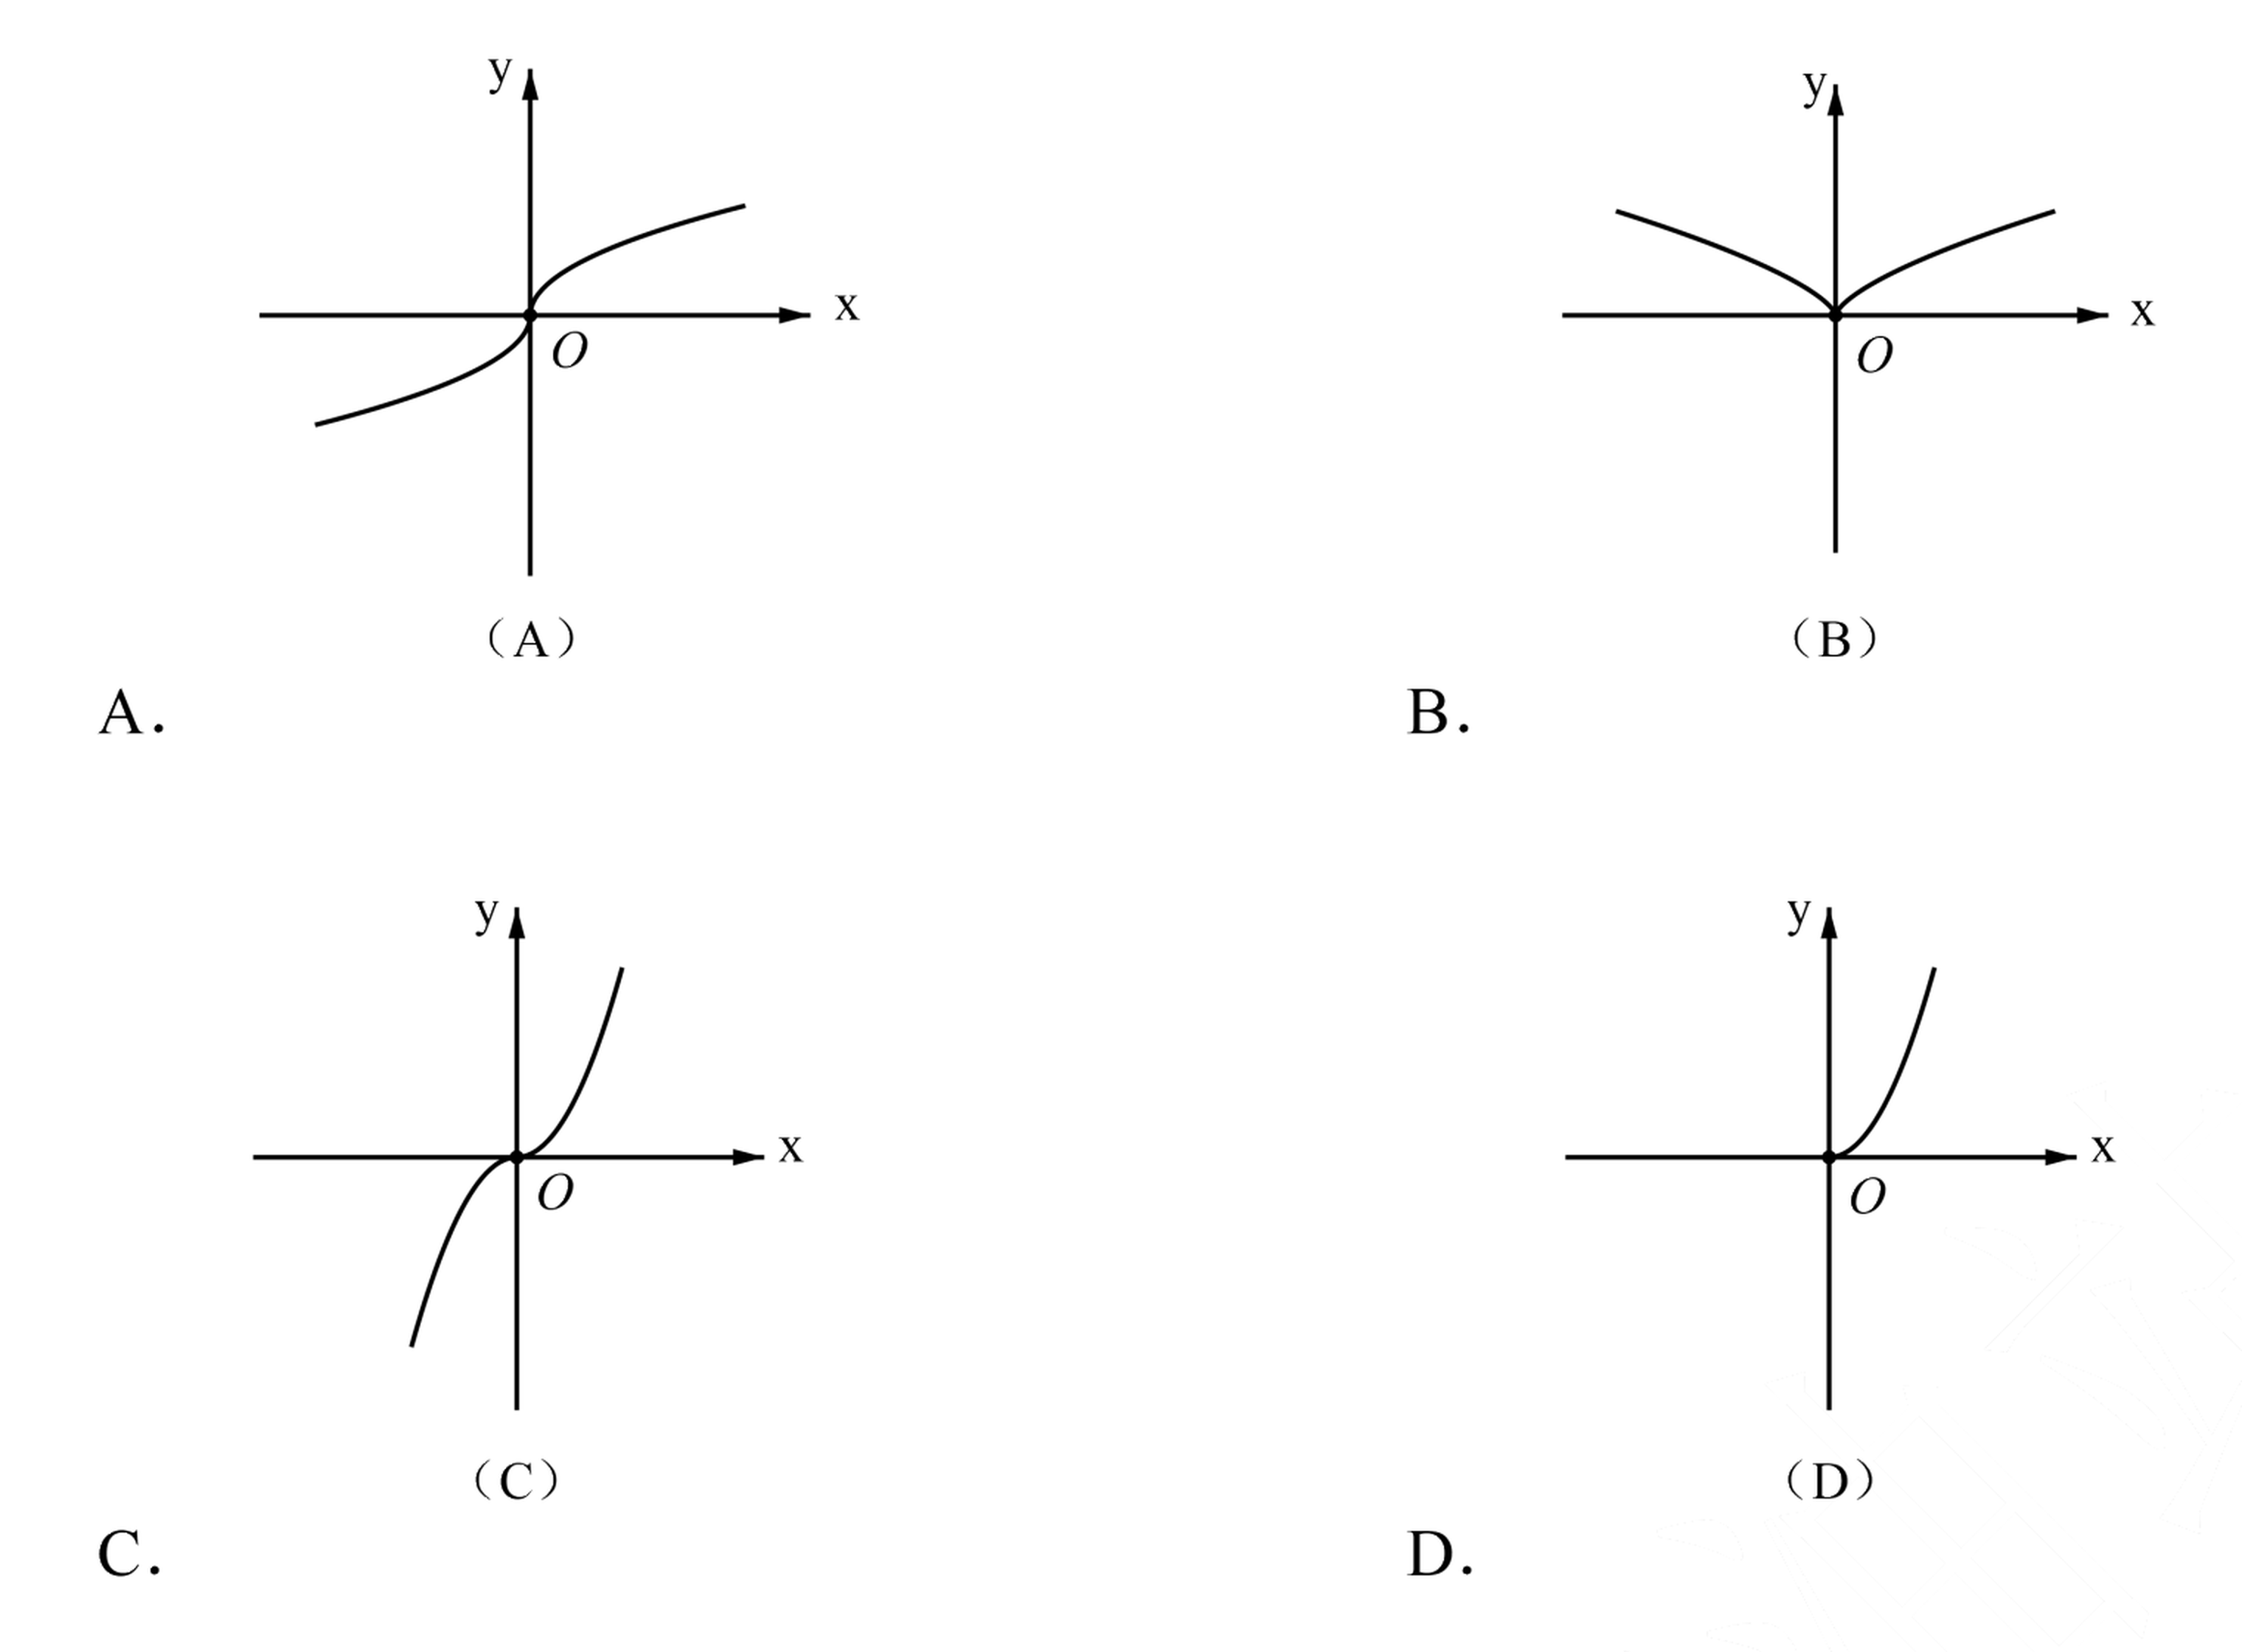
\includegraphics[width=0.80\textwidth]{figures/gao140_q14.png}
\end{center}

\ifanswer
\solbegin
\step{$f(x)=x^{\frac23}=\sqrt[3]{x^2}$ 是偶函数，且恒大于等于 $0$，故选 $B$.}
\solend
\fi

\item 设 $p$：关于 $x$ 的不等式 $x^2+ax+1>0$ 对 $x\in\R$ 恒成立，$q$：对数函数 $y=\log_{4-3a}x$ 在 $(0,+\infty)$ 上单调递减，那么 $p$ 是 $q$ 的\mbox{（\quad）}

\keepwithprev
A. 充分不必要条件\qquad B. 充要条件

C. 必要不充分条件\qquad D. 既不充分也不必要条件

\ifanswer
\solbegin
\step{$p\Leftrightarrow a^2-4<0\Leftrightarrow -2<a<2$. $q\Leftrightarrow 0<4-3a<1\Leftrightarrow 1<a<\dfrac43$.}
\step{由 $\left(1,\dfrac43\right)\subset(-2,2)$ 得 $q\Rightarrow p$；而 $a=0$ 时 $p$ 真、$q$ 假，}% 子集符号原卷印单线 $\subset$，照录
\step{故 $p$ 是 $q$ 的必要不充分条件，故选 $C$.}
\solend
\fi

\item “非空集合 $M$ 的元素都是集合 $P$ 的元素” 是假命题，现有下列命题：

(1) $M$ 的元素都不是 $P$ 的元素；(2) $M$ 中有不属于 $P$ 元素；% 原卷"不属于 P 元素"脱"的"字，照录

(3) $M$ 中有 $P$ 的元素；(4) $M$ 的元素不都是 $P$ 的元素，

其中真命题的个数是\mbox{（\quad）}

\keepwithprev
A. 1\qquad B. 2\qquad C. 3\qquad D. 4

\ifanswer
\solbegin
\step{由于 “非空集合 $M$ 的元素都是集合 $P$ 的元素” 是假命题，}
\step{得 “非空集合 $M$ 的元素至少有一个元素不属于集合 $P$” 是真命题.}
\step{则 (1) 不正确；(2) 正确；(3) $M$ 中不一定有 $P$ 的元素，例如 $M=\{a\}$，}
\step{则 $a\notin P$；(4) 正确.}
\step{综上，真命题只有 (2)(4). 故选 $B$.}
\solend
\fi

\end{enumerate}

\bigsec{三、解答题}

\begin{enumerate}
\setcounter{enumi}{16}

\item 设全集为 $\R$，集合 $A=\left\{x\mid\dfrac{2x}{x-1}\leqslant1\right\}$.

(1) 用区间表示集合 $A$；

(2) 若集合 $B=\{x\mid\lvert x+2\rvert+\lvert x-1\rvert=3\}$，求 $A\cup B$.

\ifanswer
\solbegin
\step{(1) 由 $\dfrac{2x}{x-1}\leqslant1\Leftrightarrow\dfrac{x+1}{x-1}\leqslant0$，故 $A=[-1,1)$，则 $\overline{A}=(-\infty,-1)\cup[1,+\infty)$；}
\step{(2) 由 $B=\{x\mid\lvert x+2\rvert+\lvert x-1\rvert=3\}=[-2,1]$，}
\step{结合上一问有 $A=[-1,1)$，所以 $A\cup B=B=[-2,1]$.}
\solend
\fi

\item (1) 已知指数函数 $y=a^x(a>0$ 且 $a\neq1)$ 在区间 $[-1,1]$ 上的最大值与最小值之和等于 $\dfrac52$，求实数 $a$ 的值.

(2) 已知幂函数 $y=x^{m^2+7m+10}(m\in\Z)$ 的图像关于 $y$ 轴对称，且在 $(0,+\infty)$ 上严格减. 若 $(a-1)^{m^2+7m+10}\geqslant(1+2a)^{m^2+7m+10}$. 求实数 $a$ 的取值范围.

\ifanswer
\solbegin
\step{(1) 指数函数 $y=a^x$ 在区间 $[-1,1]$ 上单调，所以 $a^1+a^{-1}=\dfrac52$，}
\step{所以 $a=2$ 或 $a=\dfrac12$；}
\step{(2) 由题意得 $m^2+7m+10<0$，所以 $-5<m<-2$，又因为 $m\in\Z$，}
\step{所以 $m=-4$ 或 $m=-3$，}
\step{当 $m=-4$ 时，$y=x^{m^2+7m+10}=x^{-2}$，为偶函数，}
\step{当 $m=-3$ 时，$y=x^{m^2+7m+10}=x^{-2}$，为偶函数，}
\step{所以 $m^2+7m+10=-2$，所以 $(a-1)^{-2}\geqslant(1+2a)^{-2}$，}
\step{所以 $\lvert a-1\rvert\leqslant\lvert 1+2a\rvert$，所以 $a\leqslant-2$ 或 $a\geqslant0$，所以 $a\in(-\infty,-2]\cup[0,+\infty)$.}
\solend
\fi

\item 设函数 $f(x)=ax^2+(1-a)x+a-2$ （$a\in\R$）.

(1) 若关于 $x$ 的不等式 $f(x)\leqslant0$ 的解集为 $\left[0,\dfrac12\right]$，求实数 $a$ 的值；

(2) 若 $a\geqslant0$，解关于 $x$ 的不等式：$f(x)<a-1$.

\ifanswer
\solbegin
\step{(1) 由解集得 $a>0$，且 $0$ 是方程 $f(x)=0$ 的根，故 $f(0)=a-2=0$，}
\step{得 $a=2$.}
\step{此时 $f(x)=2x^2-x=x(2x-1)$，$f(x)\leqslant0$ 的解集确为 $\left[0,\dfrac12\right]$.}
\step{(2) $f(x)<a-1\Leftrightarrow ax^2+(1-a)x-1<0\Leftrightarrow(x-1)(ax+1)<0$，}
\step{当 $a=0$ 时，$x-1<0$，解集为 $(-\infty,1)$.}
\step{当 $a>0$ 时，$-\dfrac1a<1$，解集为 $\left(-\dfrac1a,1\right)$.}
\solend
\fi

\item 为了保护环境，某单位采用新工艺，把二氧化碳转化为一种可利用的化工产品，已知该单位每月处理量最多不超过 $300$ 吨. 当月处理量为 $x$ 吨时，月处理成本为 $x^2-200x+40000(0<x\leqslant300)$ 元，且每处理一吨二氧化碳得到可利用的化工产品价值为 $300$ 元.

(1) 若要保证该单位每月不亏损，则每月处理量应控制在什么范围？

(2) 该单位每月处理量为多少吨时，才能使每吨的平均处理成本最低，最低为多少元？

\ifanswer
\solbegin
\step{(1) 由题意得 $S=300x-(x^2-200x+40000)$}
\step{$=-x^2+500x-40000(0<x\leqslant300)$，}
\step{令 $S\geqslant0$，即 $-x^2+500x-40000\geqslant0$，解得 $100\leqslant x\leqslant400$，}
\step{又 $0<x\leqslant300$，所以 $100\leqslant x\leqslant300$，}
\step{故要保证该单位每月不亏损，则每月处理量应控制在 $[100,300]$ 范围内；}
\step{(2) 每吨的平均出来成本为 $\dfrac yx=x+\dfrac{40000}x-200\geqslant2\sqrt{x\cdot\dfrac{40000}x}-200=200$，}% 原卷"平均出来成本"与题干"平均处理成本"措辞不一，照录
\step{当且仅当 $x=\dfrac{40000}x$，即 $x=200$ 时取等号，}
\step{所以该单位每月处理量为 $200$ 吨时，}
\step{才能使每吨的平均处理成本最低且最低为 $200$ 元.}
\solend
\fi

\item 已知函数 $y=f(x),x\in D$，若对于定义域 $D$ 内任意实数 $x,y$，不等式 $f(x)+f(y)\geqslant f(xy)$ 都成立，则称函数 $y=f(x)$ 是 $QB$ 函数，

(1) 判断函数 $f(x)=x+1$ 是否是 $QB$ 函数，并说明理由；

(2) 若函数 $g(x)=\ln(ax),x>0$ 是 $QB$ 函数，求实数 $a$ 的取值范围；

(3) 已知函数 $h(x)=a^x(a\in\R\text{ 且 }a>0)$，证明：“函数 $y=h(x)$ 是 $QB$ 函数” 的充要条件是 “ $a\in\{1\}$ ”.

\ifanswer
\solbegin
\step{(1) 不是，理由如下：因为 $f(x)=x+1$，}
\step{所以 $f(x)+f(y)\geqslant f(xy)\Leftrightarrow x+y\geqslant xy-1\Leftrightarrow(x-1)(y-1)\leqslant2$，}
\step{显然不恒成立，故不是 $QB$ 函数；}
\step{(2) 因为函数 $g(x)=\ln(ax),x>0$，则 $a>0$，}
\step{若函数 $g(x)$ 是 $QB$ 函数，则 $g(x)+g(y)\geqslant g(xy)$，}
\step{即 $\ln(ax)+\ln(ay)\geqslant\ln(axy)$，则 $\ln(a^2xy)\geqslant\ln(axy)$，得 $a^2xy\geqslant axy$，}
\step{且 $x>0,y>0$，得 $a^2\geqslant a$，解得 $a\geqslant1$ 或 $a\leqslant0$（舍去），}
\step{所以实数 $a$ 的取值范围为 $[1,+\infty)$.}
\step{(3) 若函数 $h(x)=a^x$ 是 $QB$ 函数，}
\step{当 $a>1$ 时，令 $x=y=\log_a\dfrac12$，则 $h(x)+h(y)=a^x+a^y=\dfrac12+\dfrac12=1$，}
\step{且 $h(xy)=a^{xy}=(a^x)^y=\left(\dfrac12\right)^{\log_a\frac12}=2^{\log_a2}$，}
\step{因为 $\log_a2>0$，所以 $h(xy)=2^{\log_a2}>1$，不满足 $h(x)+h(y)\geqslant h(xy)$，}
\step{不合题意；}
\step{当 $a=1$ 时，$h(x)+h(y)=a^x+a^y=1+1=2$，且 $h(xy)=a^{xy}=1$，}
\step{满足 $h(x)+h(y)\geqslant h(xy)$，符合题意；}
\step{当 $0<a<1$ 时，令 $x=\log_a2,y=2$，则 $h(x)+h(y)=a^x+a^y=2+a^2$，}
\step{且 $h(xy)=a^{xy}=(a^x)^y=2^2=4$，}
\step{因为 $0<a<1$，所以 $0<a^2<1$，得 $2<2+a^2<3$，}
\step{不满足 $h(x)+h(y)\geqslant h(xy)$，不合题意；}
\step{综上所述，$a\in\{1\}$，即充分性成立；}% 原卷"充分性/必要性"两标签与所证方向互换，照录
\step{若 $a\in\{1\}$，则 $h(x)+h(y)=a^x+a^y=1+1=2$，且 $h(xy)=a^{xy}=1$，}
\step{得 $h(x)+h(y)\geqslant h(xy)$，所以函数 $h(x)=a^x$ 是 $QB$ 函数，即必要性成立；}% 原卷"充分性/必要性"两标签与所证方向互换，照录
\step{综上所述，“函数 $y=h(x)$ 是 $QB$ 函数” 的充要条件是 “ $a\in\{1\}$ ”.}
\solend
\fi

\end{enumerate}

\end{document}
"
% 紧凑版：xelatex "\def\iscompact{1}% 高一140_甘泉外国语_期中.tex
%   —— 高一上数学"2026-2027 年甘泉外国语高一上期中"（试卷版/答案版）
% 试卷版：xelatex 高一140_甘泉外国语_期中.tex
% 答案版：xelatex "\def\isanswer{1}% 高一140_甘泉外国语_期中.tex
%   —— 高一上数学"2026-2027 年甘泉外国语高一上期中"（试卷版/答案版）
% 试卷版：xelatex 高一140_甘泉外国语_期中.tex
% 答案版：xelatex "\def\isanswer{1}% 高一140_甘泉外国语_期中.tex
%   —— 高一上数学"2026-2027 年甘泉外国语高一上期中"（试卷版/答案版）
% 试卷版：xelatex 高一140_甘泉外国语_期中.tex
% 答案版：xelatex "\def\isanswer{1}\input{高一140_甘泉外国语_期中.tex}"
% 紧凑版：xelatex "\def\iscompact{1}\input{高一140_甘泉外国语_期中.tex}"
%
% ① 原始材料：微信公众号"魔都数学加油站"文章，连载"27学年高一140"，原文标题
% "27学年高一140——2026-2027年上海市甘泉外国语高一上期中"；
% 原文链接：https://mp.weixin.qq.com/s/eflgf2Ktk1LyT9x-k-ltLw。
% 正文为 9 张 PNG 页（01、02、03、05、06、07、08 为 4762x6735；04、09 为 2560x3620，
% 同一篇各页分辨率不同，逐页按各自分辨率裁图核对），题目下印有【答案】或【解析】，为讲评版。
% 题目、解析均据原图转录；卷面粉红色水印"魔都数学加油站"及公众号页脚未录入。
% 全卷 1 幅插图：第 14 题四幅坐标函数图象选项（04 页），取原卷截图去粉色水印、去色、
% LANCZOS 放大 2 倍，四幅选项按原卷 2x2 排布（含（A）（B）（C）（D）图注与 A./B./C./D.
% 选项字母）合并裁为一张；图前按惯例加 \needvspace 守卫。
%
% 卷首标题：原卷印作"2026-2027 年甘泉外国语高一上期中"（公众号标题中的"上海市"
% 卷面标题行没有，本稿照卷面），年份区间按全稿惯例排 en dash；原卷未印副标题，
% 本卷为期中卷、跨集合与常用逻辑用语／不等式／函数三章，按题目内容标为
% "集合与常用逻辑用语、不等式、函数"（与 125／126／128／129／131／132／133 同期中卷口径相同）：
% 集合与逻辑见 Q5、Q13、Q15、Q16、Q17，不等式见 Q3、Q10、Q11、Q19、Q20，
% 函数（指数／对数／幂函数及其图象、同构与 QB 函数）见 Q4、Q6、Q7、Q8、Q12、Q14、Q18、Q21。
%
% 题号体例：本卷共 19 题——一、填空题 3—12（10 题）、二、选择题 13—16（4 题）、
% 三、解答题 17—21（5 题）。三节分别 \setcounter{enumi}{2}／{12}／{16}。
% 原卷从第 3 题起、无第 1、2 题，本稿保留原题号。
%
% ② 与原卷的排版差异：
%   ① 原文从第 3 题起，本稿保留原题号；
%   ② 原卷每题下直接印【答案】或【解析】，本稿按全稿惯例置于答案版；第 5 题只印
%      【答案】、无【解析】，提 \ans{}；第 13、14、15、16 题答案均在【解析】末句
%      "故选 …"，题干括号内留空、不另提 \ans{}；其余各题印【解析】、无独立答案段；
%      全卷无"答案印在题干括号内且无解析"的一型；
%   ③ 原卷未印副标题，本稿按"知识模块"口径补出；
%   ④ 原卷填空横线按全稿惯例排为 \blankline[4.4em]；选择题括号排 \mbox{（\quad）}、
%      每个选项段前按惯例加 \keepwithprev（四幅图选项那一枚放在 \begin{center} 之前）；
%      解答题不留作答区、不加 \anspace（原卷为讲评版，与 129／131／132／133／136 同）；
%   ⑤ 原卷数集混排：斜体 $R$（Q9、Q12、Q15 等）与黑体／黑板粗体 $R$（Q15、Q17、
%      Q19、Q21）、粗体 $Z$（Q18），按全稿惯例统一改 \R／\Z；空集记号 \varnothing；
%      绝对值排 \lvert…\rvert，集合描述竖线排 \mid；不等号按全稿惯例排 \leqslant／\geqslant；
%      补集照原卷上划线排 \overline{A}；
%   ⑥ 子题标号 (1)(2)(3)(4) 原卷印半角括号，照录（与 131／132／133／134／136 同口径）；
%      括注原卷全角／半角混用，逐处照录：Q8"（结果用 a,b 表示）"、Q19"（a∈R）"、
%      Q21 (2)"（舍去）"印全角，Q18"$a^x(a>0$ 且 $a\neq1)$"、Q20"$40000(0<x\leqslant300)$"、
%      Q21 (3)"($a\in\R$ 且 $a>0$)"及 (0,+∞)、2(a>0) 等数学式内括注印半角；
%   ⑦ 数学式内半角逗号照录（如 Q8"$\lg2=a,10^b=3$"、Q11"$-2,3,4,\cdots,2027$"、
%      Q12"$x_1,x_2$"、Q19"$f(x)=ax^2+(1-a)x+a-2$"、Q21"$x>0,y>0$"）；
%      原卷行末西文句点照录（Q20 题干"300 吨. 当月处理量为 x 吨时"），行中全角逗号照录；
%   ⑧ 一幅插图：第 14 题四幅坐标函数图象选项合并裁为一张 \includegraphics
%      （题前 \needvspace{9cm}）。Q14 是"二、选择题"节内带大图块的第二题
%      （Q13 为节首题但无图），另在 \bigsec{二、选择题} 之前加 \needvspace{11cm}
%      连节标题一起量——守卫必须放在 \bigsec 之前，放标题之后会让"二、选择题"
%      孤立在页末（B 类，照 高一26／40／59／136 成例）；三版切页审计均"合计异常：无"；
%   ⑨ 跨页续印按题合并：Q9 题干在 01 页、解析续至 02 页；Q11 题干与解析前 3 行在 02 页、
%      后 2 行在 03 页；Q14 题干在 03 页末、四幅图与【解析】在 04 页；Q16 题干四条命题
%      在 04 页、选项与【解析】在 05 页；Q18 解析 (1) 首行在 05 页、其余 7 行在 06 页；
%      Q20 题干在 06 页末、"300 元."与两小问及【解析】在 07 页；Q21 解析跨 07—09 页
%      （末 3 行在 09 页）；本稿按题连排，不丢行；
%   ⑩ 题干中的中文弯引号按原卷照录，注释内一律 ASCII 引号；原卷"图像／图象"
%      两种写法混用，逐处照录（Q7、Q18 作"图像"，Q14 作"图象"）；
%   ⑪ 原卷无红色加粗标签（【解析】【答案】均黑色印刷），故本卷未用 \stepm。
%
% 判别式字形：全卷仅第 9 题【解析】"经验证得"cases 块出现两处判别式
%   "$\Delta=p^2-4q>0$"与"$\Delta'=q^2-4p>0$"，原卷两处均印等腰、偏高的
%   三角 $\Delta$（带撇的为 $\Delta'$），逐处放大核对并照录 \Delta、\Delta'；
%   全卷未出现扁等边三角 \triangle。
%
% 子集符号：第 15 题【解析】"由 (1,4/3)⊂(-2,2) 得 q⇒p"一处原卷印单线 $\subset$
%   （不带下划线），逐处放大核对、照录 \subset；全卷未出现带下划线的 \subseteq。
%
% 原卷存疑照录（均照录未改，正文对应处另有 % 注）：
%   第 16 题 (2) 命题"$M$ 中有不属于 $P$ 元素"中"不属于 $P$ 元素"脱"的"字，照录；
%   第 20 题题干 (2) 作"每吨的平均处理成本"、而【解析】(2) 作"每吨的平均出来成本"，
%      "出来"疑为"处理"之误，两处措辞照录不统一；
%   第 21 题 (3)【解析】"综上所述，$a\in\{1\}$，即充分性成立"与"即必要性成立"
%      两处标签与所证方向互换（按充要条件的通常口径），照录。
%
% 行数复核：一条 \step = 原卷解析的一个印刷行，cases 块作一个印刷行计。逐题数 \step
%   条数，合计 92 条（Q3：2；Q4：1；Q5：0；Q6：2；Q7：1；Q8：1；Q9：7；Q10：5；
%   Q11：5；Q12：4；Q13：6；Q14：1；Q15：3；Q16：5；Q17：3；Q18：8；Q19：6；
%   Q20：9；Q21：23），与原卷印刷行逐题相等。第 5 题只印【答案】、提 \ans{}，
%   不计入 \step 账；第 13、14、15、16 题答案在解析末句"故选 …"，括号内留空、
%   不另提 \ans{}；答案版【答案】/【解析】标记数 = 19（1 个 \ans + 18 个 \solbegin）
%   = 全卷题数。
%
\documentclass[a4paper,11pt]{article}
\usepackage{common}

\begin{document}

\examtitlest[3]{2026--2027 年甘泉外国语高一上期中}{集合与常用逻辑用语、不等式、函数}

\bigsec{一、填空题}

\begin{enumerate}
\setcounter{enumi}{2}

\item 不等式 $x^2-2x-3<0$ 的解集为\blankline[4.4em].

\ifanswer
\solbegin
\step{方程 $x^2-2x-3=0$ 的实数根是 $x_1=-1$，$x_2=3$；}
\step{所以不等式 $x^2-2x-3<0$ 的解集为 $\{x\mid -1<x<3\}$.}
\solend
\fi

\item 根式 $\sqrt{x\sqrt{x}}(x>0)$ 的指数幂形式为\blankline[4.4em].

\ifanswer
\solbegin
\step{$\sqrt{x\sqrt{x}}=\sqrt{x\cdot x^{\frac12}}=\sqrt{x^{\frac32}}=x^{\frac34}$.}
\solend
\fi

\item 陈述句 “ $x>1$ 或 $y>1$ ” 的否定形式是\blankline[4.4em].

\ifanswer
\ans{$x\leqslant1$ 且 $y\leqslant1$}
\fi

\item 若 $x<0$ 时，指数函数 $y=(a-1)^x$ 的值总大于 $1$，则实数 $a$ 的取值范围是\blankline[4.4em].

\ifanswer
\solbegin
\step{由题意得 $(a-1)^x>1$ 在 $(-\infty,0)$ 上恒成立，则 $0<a-1<1$，解得 $1<a<2$.}
\step{故实数 $a$ 的取值范围是 $(1,2)$.}
\solend
\fi

\item 若 $f(x)=\log_a(x-1)$，对任意 $a>0$ 且 $a\neq1$，函数 $y=f(x)$ 的图像必过定点\blankline[4.4em].

\ifanswer
\solbegin
\step{令 $x-1=1$，即 $x=2$，此时 $f(2)=0$，即函数图像过定点 $(2,0)$.}
\solend
\fi

\item 已知 $\lg 2=a,10^b=3$，则 $\log_6 2=$\blankline[4.4em]（结果用 $a,b$ 表示）.

\ifanswer
\solbegin
\step{由 $10^b=3$，得 $b=\lg 3$，则 $\log_6 2=\dfrac{\lg 2}{\lg 6}=\dfrac{\lg 2}{\lg 2+\lg 3}=\dfrac{a}{a+b}$.}
\solend
\fi

\item 已知 $p$、$q\in\R$，$x_1$、$x_2$ 是关于 $x$ 的方程 $x^2+px+q=0$ 的两实根，$x_1+1$、$x_2+1$ 是关于 $x$ 的方程 $x^2+qx+p=0$ 的两实根，则 $pq=$\blankline[4.4em].

\ifanswer
\solbegin
\step{因为 $x_1$、$x_2$ 是关于 $x$ 的方程 $x^2+px+q=0$ 的两实根，}
\step{由韦达定理得 $x_1+x_2=-p$，$x_1\cdot x_2=q$，}
\step{因为 $x_1+1$、$x_2+1$ 是关于 $x$ 的方程 $x^2+qx+p=0$ 的两实根，}
\step{由韦达定理得 $x_1+1+x_2+1=-q$，$(x_1+1)(x_2+1)=p$，}
\step{即 $x_1+x_2=-q-2$，$x_1+x_2+x_1x_2=p-1$，又 $x_1+x_2=-p$，$x_1\cdot x_2=q$，}
\step{所以 $\begin{cases}-p=-q-2\\-p+q=p-1\end{cases}$，解得 $\begin{cases}p=-1\\q=-3\end{cases}$，经验证得 $\begin{cases}\Delta=p^2-4q>0\\\Delta'=q^2-4p>0\end{cases}$，}% 判别式原卷印高三角 $\Delta$、$\Delta'$，照录
\step{则 $pq=3$.}
\solend
\fi

\item 对于 $x\in\R$，不等式 $\lvert 3-x\rvert+\lvert 1+x\rvert\geqslant a^2-3a$ 恒成立，则实数 $a$ 的取值范围是\blankline[4.4em].

\ifanswer
\solbegin
\step{对于 $x\in\R$，不等式 $\lvert 3-x\rvert+\lvert 1+x\rvert\geqslant a^2-3a$ 恒成立，}
\step{即 $\lvert 3-x\rvert+\lvert 1+x\rvert$ 的最小值大于或等于 $a^2-3a$，}
\step{$\lvert 3-x\rvert+\lvert 1+x\rvert$ 表示数轴上的 $x$ 对应点到 $3$ 和 $-1$ 对应点的距离之和，}
\step{它的最小值为 $4$，故 $4\geqslant a^2-3a$，即 $a^2-3a-4\leqslant0$，解得 $-1\leqslant a\leqslant4$，}
\step{故实数 $a$ 的取值范围是 $[-1,4]$.}
\solend
\fi

\item 已知同时满足不等式 $x^2-x-2>0$ 和 $2x^2+(5+2a)x+5a<0$ 的 $x$ 的整数值只有 $2026$ 个，则实数 $a$ 的取值范围是\blankline[4.4em].

\ifanswer
\solbegin
\step{整数 $x$ 须满足 $x\leqslant-2$ 或 $x\geqslant3$，且 $(2x+5)(x+a)<0$.}
\step{当 $a<\dfrac52$ 时，需使整数解恰为 $-2,3,4,\cdots,2027$，即 $2027<-a\leqslant2028$.}
\step{当 $a>\dfrac52$ 时，需使整数解恰为 $-2028,-2027,\cdots,-3$，即 $2028<a\leqslant2029$；}
\step{$a=\dfrac52$ 时无解.}
\step{故 $a\in[-2028,-2027)\cup(2028,2029]$.}
\solend
\fi

\item 同构式通俗讲是结构相同的表达式，如：$f(x)=x+e^x$，$f(\ln x)=\ln x+e^{\ln x}=\ln x+x$，称 $x+e^x$ 与 $\ln x+x$ 为同构式. 已知实数 $x_1,x_2$ 满足 $e^{x_1}+x_1=8,\ln\sqrt[5]{5x_2+3}+x_2=1$，则 $x_1+5x_2=$\blankline[4.4em].

\ifanswer
\solbegin
\step{函数 $f(x)=x+e^x$ 在 $\R$ 上严格增，且 $f(x_1)=x_1+e^{x_1}=8$，}
\step{由 $\ln\sqrt[5]{5x_2+3}+x_2=1$，得 $\ln(5x_2+3)+5x_2=5$，则 $\ln(5x_2+3)+5x_2+3=8$，}
\step{即 $f(\ln(5x_2+3))=8$，因此 $f(\ln(5x_2+3))=8=f(x_1)$，则 $x_1=\ln(5x_2+3)$，}
\step{所以 $x_1+5x_2=\ln(5x_2+3)+5x_2=5$.}
\solend
\fi

\end{enumerate}

% 第 14 题四幅图是"二、选择题"节内的大图块；守卫须放在 \bigsec 之前连节标题一起量，
% 否则"二、选择题"会孤立在页末（B 类，照 高一26／40／59／136 成例）
\needvspace{11cm}
\bigsec{二、选择题}

\begin{enumerate}
\setcounter{enumi}{12}

\item 设 $a$、$b$ 为实数，则 “ $a>b>0$ ” 的一个充分非必要条件是\mbox{（\quad）}

\keepwithprev
A. $\sqrt{a-1}>\sqrt{b-1}$\qquad B. $a^2>b^2$

C. $\dfrac1b>\dfrac1a$\qquad D. $a-b>b-a$

\ifanswer
\solbegin
\step{由 $\sqrt{a-1}>\sqrt{b-1}$ 得 $a>b\geqslant1$，故 $a>b>0$，反之不成立，满足题意；}
\step{由 $a^2>b^2$，则 $\lvert a\rvert>\lvert b\rvert$，推不出 $a>b>0$，反向可推出，不满足；}
\step{由 $\dfrac1b>\dfrac1a$，则 $a>b>0$ 或 $b>0>a$ 或 $0>a>b$，推不出 $a>b>0$，}
\step{反向可推出，不满足；}
\step{由 $a-b>b-a$，则 $a>b$，推不出 $a>b>0$，反向可推出，不满足；}
\step{故选 $A$.}
\solend
\fi

% 第 14 题四幅坐标函数图象选项是一整块，守卫放在 \item 之前
\needvspace{9cm}
\item 幂函数 $f(x)=x^{\frac23}$ 的图象大致为\mbox{（\quad）}

\keepwithprev
\begin{center}
% 四幅坐标函数图象选项取原卷 04 页截图去粉色水印、去色，按原卷 2x2 排布合并为一张
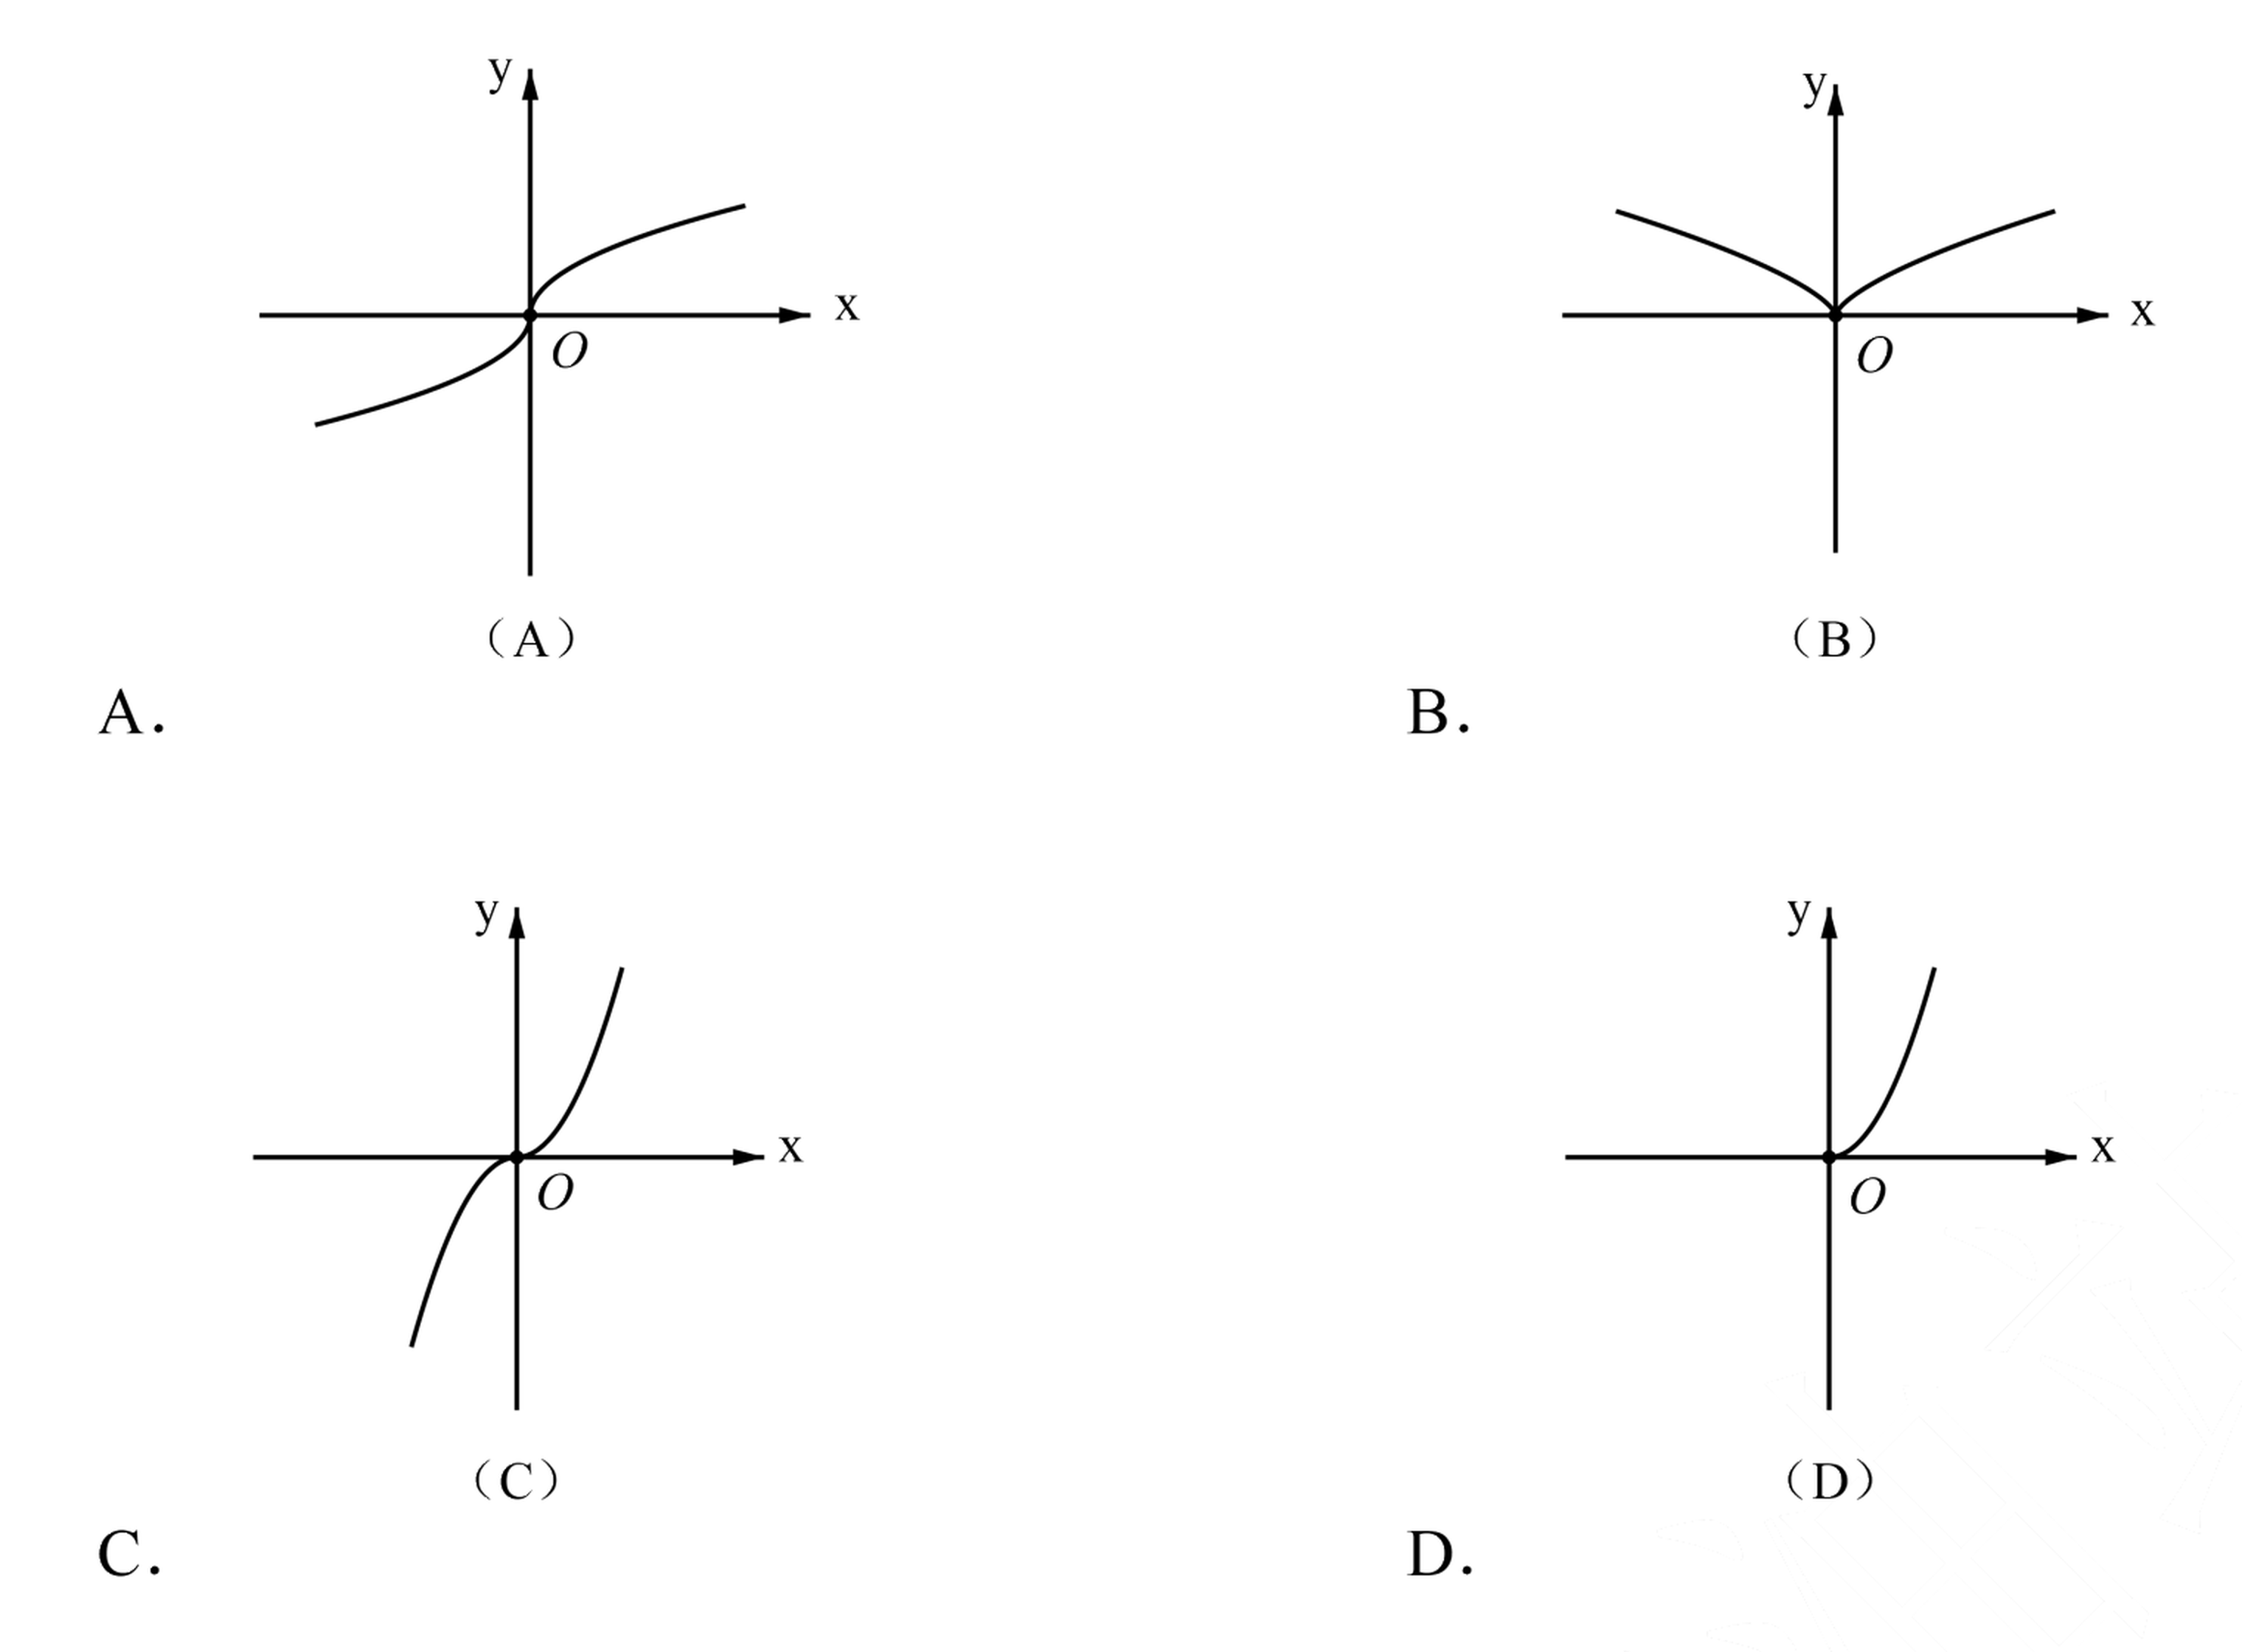
\includegraphics[width=0.80\textwidth]{figures/gao140_q14.png}
\end{center}

\ifanswer
\solbegin
\step{$f(x)=x^{\frac23}=\sqrt[3]{x^2}$ 是偶函数，且恒大于等于 $0$，故选 $B$.}
\solend
\fi

\item 设 $p$：关于 $x$ 的不等式 $x^2+ax+1>0$ 对 $x\in\R$ 恒成立，$q$：对数函数 $y=\log_{4-3a}x$ 在 $(0,+\infty)$ 上单调递减，那么 $p$ 是 $q$ 的\mbox{（\quad）}

\keepwithprev
A. 充分不必要条件\qquad B. 充要条件

C. 必要不充分条件\qquad D. 既不充分也不必要条件

\ifanswer
\solbegin
\step{$p\Leftrightarrow a^2-4<0\Leftrightarrow -2<a<2$. $q\Leftrightarrow 0<4-3a<1\Leftrightarrow 1<a<\dfrac43$.}
\step{由 $\left(1,\dfrac43\right)\subset(-2,2)$ 得 $q\Rightarrow p$；而 $a=0$ 时 $p$ 真、$q$ 假，}% 子集符号原卷印单线 $\subset$，照录
\step{故 $p$ 是 $q$ 的必要不充分条件，故选 $C$.}
\solend
\fi

\item “非空集合 $M$ 的元素都是集合 $P$ 的元素” 是假命题，现有下列命题：

(1) $M$ 的元素都不是 $P$ 的元素；(2) $M$ 中有不属于 $P$ 元素；% 原卷"不属于 P 元素"脱"的"字，照录

(3) $M$ 中有 $P$ 的元素；(4) $M$ 的元素不都是 $P$ 的元素，

其中真命题的个数是\mbox{（\quad）}

\keepwithprev
A. 1\qquad B. 2\qquad C. 3\qquad D. 4

\ifanswer
\solbegin
\step{由于 “非空集合 $M$ 的元素都是集合 $P$ 的元素” 是假命题，}
\step{得 “非空集合 $M$ 的元素至少有一个元素不属于集合 $P$” 是真命题.}
\step{则 (1) 不正确；(2) 正确；(3) $M$ 中不一定有 $P$ 的元素，例如 $M=\{a\}$，}
\step{则 $a\notin P$；(4) 正确.}
\step{综上，真命题只有 (2)(4). 故选 $B$.}
\solend
\fi

\end{enumerate}

\bigsec{三、解答题}

\begin{enumerate}
\setcounter{enumi}{16}

\item 设全集为 $\R$，集合 $A=\left\{x\mid\dfrac{2x}{x-1}\leqslant1\right\}$.

(1) 用区间表示集合 $A$；

(2) 若集合 $B=\{x\mid\lvert x+2\rvert+\lvert x-1\rvert=3\}$，求 $A\cup B$.

\ifanswer
\solbegin
\step{(1) 由 $\dfrac{2x}{x-1}\leqslant1\Leftrightarrow\dfrac{x+1}{x-1}\leqslant0$，故 $A=[-1,1)$，则 $\overline{A}=(-\infty,-1)\cup[1,+\infty)$；}
\step{(2) 由 $B=\{x\mid\lvert x+2\rvert+\lvert x-1\rvert=3\}=[-2,1]$，}
\step{结合上一问有 $A=[-1,1)$，所以 $A\cup B=B=[-2,1]$.}
\solend
\fi

\item (1) 已知指数函数 $y=a^x(a>0$ 且 $a\neq1)$ 在区间 $[-1,1]$ 上的最大值与最小值之和等于 $\dfrac52$，求实数 $a$ 的值.

(2) 已知幂函数 $y=x^{m^2+7m+10}(m\in\Z)$ 的图像关于 $y$ 轴对称，且在 $(0,+\infty)$ 上严格减. 若 $(a-1)^{m^2+7m+10}\geqslant(1+2a)^{m^2+7m+10}$. 求实数 $a$ 的取值范围.

\ifanswer
\solbegin
\step{(1) 指数函数 $y=a^x$ 在区间 $[-1,1]$ 上单调，所以 $a^1+a^{-1}=\dfrac52$，}
\step{所以 $a=2$ 或 $a=\dfrac12$；}
\step{(2) 由题意得 $m^2+7m+10<0$，所以 $-5<m<-2$，又因为 $m\in\Z$，}
\step{所以 $m=-4$ 或 $m=-3$，}
\step{当 $m=-4$ 时，$y=x^{m^2+7m+10}=x^{-2}$，为偶函数，}
\step{当 $m=-3$ 时，$y=x^{m^2+7m+10}=x^{-2}$，为偶函数，}
\step{所以 $m^2+7m+10=-2$，所以 $(a-1)^{-2}\geqslant(1+2a)^{-2}$，}
\step{所以 $\lvert a-1\rvert\leqslant\lvert 1+2a\rvert$，所以 $a\leqslant-2$ 或 $a\geqslant0$，所以 $a\in(-\infty,-2]\cup[0,+\infty)$.}
\solend
\fi

\item 设函数 $f(x)=ax^2+(1-a)x+a-2$ （$a\in\R$）.

(1) 若关于 $x$ 的不等式 $f(x)\leqslant0$ 的解集为 $\left[0,\dfrac12\right]$，求实数 $a$ 的值；

(2) 若 $a\geqslant0$，解关于 $x$ 的不等式：$f(x)<a-1$.

\ifanswer
\solbegin
\step{(1) 由解集得 $a>0$，且 $0$ 是方程 $f(x)=0$ 的根，故 $f(0)=a-2=0$，}
\step{得 $a=2$.}
\step{此时 $f(x)=2x^2-x=x(2x-1)$，$f(x)\leqslant0$ 的解集确为 $\left[0,\dfrac12\right]$.}
\step{(2) $f(x)<a-1\Leftrightarrow ax^2+(1-a)x-1<0\Leftrightarrow(x-1)(ax+1)<0$，}
\step{当 $a=0$ 时，$x-1<0$，解集为 $(-\infty,1)$.}
\step{当 $a>0$ 时，$-\dfrac1a<1$，解集为 $\left(-\dfrac1a,1\right)$.}
\solend
\fi

\item 为了保护环境，某单位采用新工艺，把二氧化碳转化为一种可利用的化工产品，已知该单位每月处理量最多不超过 $300$ 吨. 当月处理量为 $x$ 吨时，月处理成本为 $x^2-200x+40000(0<x\leqslant300)$ 元，且每处理一吨二氧化碳得到可利用的化工产品价值为 $300$ 元.

(1) 若要保证该单位每月不亏损，则每月处理量应控制在什么范围？

(2) 该单位每月处理量为多少吨时，才能使每吨的平均处理成本最低，最低为多少元？

\ifanswer
\solbegin
\step{(1) 由题意得 $S=300x-(x^2-200x+40000)$}
\step{$=-x^2+500x-40000(0<x\leqslant300)$，}
\step{令 $S\geqslant0$，即 $-x^2+500x-40000\geqslant0$，解得 $100\leqslant x\leqslant400$，}
\step{又 $0<x\leqslant300$，所以 $100\leqslant x\leqslant300$，}
\step{故要保证该单位每月不亏损，则每月处理量应控制在 $[100,300]$ 范围内；}
\step{(2) 每吨的平均出来成本为 $\dfrac yx=x+\dfrac{40000}x-200\geqslant2\sqrt{x\cdot\dfrac{40000}x}-200=200$，}% 原卷"平均出来成本"与题干"平均处理成本"措辞不一，照录
\step{当且仅当 $x=\dfrac{40000}x$，即 $x=200$ 时取等号，}
\step{所以该单位每月处理量为 $200$ 吨时，}
\step{才能使每吨的平均处理成本最低且最低为 $200$ 元.}
\solend
\fi

\item 已知函数 $y=f(x),x\in D$，若对于定义域 $D$ 内任意实数 $x,y$，不等式 $f(x)+f(y)\geqslant f(xy)$ 都成立，则称函数 $y=f(x)$ 是 $QB$ 函数，

(1) 判断函数 $f(x)=x+1$ 是否是 $QB$ 函数，并说明理由；

(2) 若函数 $g(x)=\ln(ax),x>0$ 是 $QB$ 函数，求实数 $a$ 的取值范围；

(3) 已知函数 $h(x)=a^x(a\in\R\text{ 且 }a>0)$，证明：“函数 $y=h(x)$ 是 $QB$ 函数” 的充要条件是 “ $a\in\{1\}$ ”.

\ifanswer
\solbegin
\step{(1) 不是，理由如下：因为 $f(x)=x+1$，}
\step{所以 $f(x)+f(y)\geqslant f(xy)\Leftrightarrow x+y\geqslant xy-1\Leftrightarrow(x-1)(y-1)\leqslant2$，}
\step{显然不恒成立，故不是 $QB$ 函数；}
\step{(2) 因为函数 $g(x)=\ln(ax),x>0$，则 $a>0$，}
\step{若函数 $g(x)$ 是 $QB$ 函数，则 $g(x)+g(y)\geqslant g(xy)$，}
\step{即 $\ln(ax)+\ln(ay)\geqslant\ln(axy)$，则 $\ln(a^2xy)\geqslant\ln(axy)$，得 $a^2xy\geqslant axy$，}
\step{且 $x>0,y>0$，得 $a^2\geqslant a$，解得 $a\geqslant1$ 或 $a\leqslant0$（舍去），}
\step{所以实数 $a$ 的取值范围为 $[1,+\infty)$.}
\step{(3) 若函数 $h(x)=a^x$ 是 $QB$ 函数，}
\step{当 $a>1$ 时，令 $x=y=\log_a\dfrac12$，则 $h(x)+h(y)=a^x+a^y=\dfrac12+\dfrac12=1$，}
\step{且 $h(xy)=a^{xy}=(a^x)^y=\left(\dfrac12\right)^{\log_a\frac12}=2^{\log_a2}$，}
\step{因为 $\log_a2>0$，所以 $h(xy)=2^{\log_a2}>1$，不满足 $h(x)+h(y)\geqslant h(xy)$，}
\step{不合题意；}
\step{当 $a=1$ 时，$h(x)+h(y)=a^x+a^y=1+1=2$，且 $h(xy)=a^{xy}=1$，}
\step{满足 $h(x)+h(y)\geqslant h(xy)$，符合题意；}
\step{当 $0<a<1$ 时，令 $x=\log_a2,y=2$，则 $h(x)+h(y)=a^x+a^y=2+a^2$，}
\step{且 $h(xy)=a^{xy}=(a^x)^y=2^2=4$，}
\step{因为 $0<a<1$，所以 $0<a^2<1$，得 $2<2+a^2<3$，}
\step{不满足 $h(x)+h(y)\geqslant h(xy)$，不合题意；}
\step{综上所述，$a\in\{1\}$，即充分性成立；}% 原卷"充分性/必要性"两标签与所证方向互换，照录
\step{若 $a\in\{1\}$，则 $h(x)+h(y)=a^x+a^y=1+1=2$，且 $h(xy)=a^{xy}=1$，}
\step{得 $h(x)+h(y)\geqslant h(xy)$，所以函数 $h(x)=a^x$ 是 $QB$ 函数，即必要性成立；}% 原卷"充分性/必要性"两标签与所证方向互换，照录
\step{综上所述，“函数 $y=h(x)$ 是 $QB$ 函数” 的充要条件是 “ $a\in\{1\}$ ”.}
\solend
\fi

\end{enumerate}

\end{document}
"
% 紧凑版：xelatex "\def\iscompact{1}% 高一140_甘泉外国语_期中.tex
%   —— 高一上数学"2026-2027 年甘泉外国语高一上期中"（试卷版/答案版）
% 试卷版：xelatex 高一140_甘泉外国语_期中.tex
% 答案版：xelatex "\def\isanswer{1}\input{高一140_甘泉外国语_期中.tex}"
% 紧凑版：xelatex "\def\iscompact{1}\input{高一140_甘泉外国语_期中.tex}"
%
% ① 原始材料：微信公众号"魔都数学加油站"文章，连载"27学年高一140"，原文标题
% "27学年高一140——2026-2027年上海市甘泉外国语高一上期中"；
% 原文链接：https://mp.weixin.qq.com/s/eflgf2Ktk1LyT9x-k-ltLw。
% 正文为 9 张 PNG 页（01、02、03、05、06、07、08 为 4762x6735；04、09 为 2560x3620，
% 同一篇各页分辨率不同，逐页按各自分辨率裁图核对），题目下印有【答案】或【解析】，为讲评版。
% 题目、解析均据原图转录；卷面粉红色水印"魔都数学加油站"及公众号页脚未录入。
% 全卷 1 幅插图：第 14 题四幅坐标函数图象选项（04 页），取原卷截图去粉色水印、去色、
% LANCZOS 放大 2 倍，四幅选项按原卷 2x2 排布（含（A）（B）（C）（D）图注与 A./B./C./D.
% 选项字母）合并裁为一张；图前按惯例加 \needvspace 守卫。
%
% 卷首标题：原卷印作"2026-2027 年甘泉外国语高一上期中"（公众号标题中的"上海市"
% 卷面标题行没有，本稿照卷面），年份区间按全稿惯例排 en dash；原卷未印副标题，
% 本卷为期中卷、跨集合与常用逻辑用语／不等式／函数三章，按题目内容标为
% "集合与常用逻辑用语、不等式、函数"（与 125／126／128／129／131／132／133 同期中卷口径相同）：
% 集合与逻辑见 Q5、Q13、Q15、Q16、Q17，不等式见 Q3、Q10、Q11、Q19、Q20，
% 函数（指数／对数／幂函数及其图象、同构与 QB 函数）见 Q4、Q6、Q7、Q8、Q12、Q14、Q18、Q21。
%
% 题号体例：本卷共 19 题——一、填空题 3—12（10 题）、二、选择题 13—16（4 题）、
% 三、解答题 17—21（5 题）。三节分别 \setcounter{enumi}{2}／{12}／{16}。
% 原卷从第 3 题起、无第 1、2 题，本稿保留原题号。
%
% ② 与原卷的排版差异：
%   ① 原文从第 3 题起，本稿保留原题号；
%   ② 原卷每题下直接印【答案】或【解析】，本稿按全稿惯例置于答案版；第 5 题只印
%      【答案】、无【解析】，提 \ans{}；第 13、14、15、16 题答案均在【解析】末句
%      "故选 …"，题干括号内留空、不另提 \ans{}；其余各题印【解析】、无独立答案段；
%      全卷无"答案印在题干括号内且无解析"的一型；
%   ③ 原卷未印副标题，本稿按"知识模块"口径补出；
%   ④ 原卷填空横线按全稿惯例排为 \blankline[4.4em]；选择题括号排 \mbox{（\quad）}、
%      每个选项段前按惯例加 \keepwithprev（四幅图选项那一枚放在 \begin{center} 之前）；
%      解答题不留作答区、不加 \anspace（原卷为讲评版，与 129／131／132／133／136 同）；
%   ⑤ 原卷数集混排：斜体 $R$（Q9、Q12、Q15 等）与黑体／黑板粗体 $R$（Q15、Q17、
%      Q19、Q21）、粗体 $Z$（Q18），按全稿惯例统一改 \R／\Z；空集记号 \varnothing；
%      绝对值排 \lvert…\rvert，集合描述竖线排 \mid；不等号按全稿惯例排 \leqslant／\geqslant；
%      补集照原卷上划线排 \overline{A}；
%   ⑥ 子题标号 (1)(2)(3)(4) 原卷印半角括号，照录（与 131／132／133／134／136 同口径）；
%      括注原卷全角／半角混用，逐处照录：Q8"（结果用 a,b 表示）"、Q19"（a∈R）"、
%      Q21 (2)"（舍去）"印全角，Q18"$a^x(a>0$ 且 $a\neq1)$"、Q20"$40000(0<x\leqslant300)$"、
%      Q21 (3)"($a\in\R$ 且 $a>0$)"及 (0,+∞)、2(a>0) 等数学式内括注印半角；
%   ⑦ 数学式内半角逗号照录（如 Q8"$\lg2=a,10^b=3$"、Q11"$-2,3,4,\cdots,2027$"、
%      Q12"$x_1,x_2$"、Q19"$f(x)=ax^2+(1-a)x+a-2$"、Q21"$x>0,y>0$"）；
%      原卷行末西文句点照录（Q20 题干"300 吨. 当月处理量为 x 吨时"），行中全角逗号照录；
%   ⑧ 一幅插图：第 14 题四幅坐标函数图象选项合并裁为一张 \includegraphics
%      （题前 \needvspace{9cm}）。Q14 是"二、选择题"节内带大图块的第二题
%      （Q13 为节首题但无图），另在 \bigsec{二、选择题} 之前加 \needvspace{11cm}
%      连节标题一起量——守卫必须放在 \bigsec 之前，放标题之后会让"二、选择题"
%      孤立在页末（B 类，照 高一26／40／59／136 成例）；三版切页审计均"合计异常：无"；
%   ⑨ 跨页续印按题合并：Q9 题干在 01 页、解析续至 02 页；Q11 题干与解析前 3 行在 02 页、
%      后 2 行在 03 页；Q14 题干在 03 页末、四幅图与【解析】在 04 页；Q16 题干四条命题
%      在 04 页、选项与【解析】在 05 页；Q18 解析 (1) 首行在 05 页、其余 7 行在 06 页；
%      Q20 题干在 06 页末、"300 元."与两小问及【解析】在 07 页；Q21 解析跨 07—09 页
%      （末 3 行在 09 页）；本稿按题连排，不丢行；
%   ⑩ 题干中的中文弯引号按原卷照录，注释内一律 ASCII 引号；原卷"图像／图象"
%      两种写法混用，逐处照录（Q7、Q18 作"图像"，Q14 作"图象"）；
%   ⑪ 原卷无红色加粗标签（【解析】【答案】均黑色印刷），故本卷未用 \stepm。
%
% 判别式字形：全卷仅第 9 题【解析】"经验证得"cases 块出现两处判别式
%   "$\Delta=p^2-4q>0$"与"$\Delta'=q^2-4p>0$"，原卷两处均印等腰、偏高的
%   三角 $\Delta$（带撇的为 $\Delta'$），逐处放大核对并照录 \Delta、\Delta'；
%   全卷未出现扁等边三角 \triangle。
%
% 子集符号：第 15 题【解析】"由 (1,4/3)⊂(-2,2) 得 q⇒p"一处原卷印单线 $\subset$
%   （不带下划线），逐处放大核对、照录 \subset；全卷未出现带下划线的 \subseteq。
%
% 原卷存疑照录（均照录未改，正文对应处另有 % 注）：
%   第 16 题 (2) 命题"$M$ 中有不属于 $P$ 元素"中"不属于 $P$ 元素"脱"的"字，照录；
%   第 20 题题干 (2) 作"每吨的平均处理成本"、而【解析】(2) 作"每吨的平均出来成本"，
%      "出来"疑为"处理"之误，两处措辞照录不统一；
%   第 21 题 (3)【解析】"综上所述，$a\in\{1\}$，即充分性成立"与"即必要性成立"
%      两处标签与所证方向互换（按充要条件的通常口径），照录。
%
% 行数复核：一条 \step = 原卷解析的一个印刷行，cases 块作一个印刷行计。逐题数 \step
%   条数，合计 92 条（Q3：2；Q4：1；Q5：0；Q6：2；Q7：1；Q8：1；Q9：7；Q10：5；
%   Q11：5；Q12：4；Q13：6；Q14：1；Q15：3；Q16：5；Q17：3；Q18：8；Q19：6；
%   Q20：9；Q21：23），与原卷印刷行逐题相等。第 5 题只印【答案】、提 \ans{}，
%   不计入 \step 账；第 13、14、15、16 题答案在解析末句"故选 …"，括号内留空、
%   不另提 \ans{}；答案版【答案】/【解析】标记数 = 19（1 个 \ans + 18 个 \solbegin）
%   = 全卷题数。
%
\documentclass[a4paper,11pt]{article}
\usepackage{common}

\begin{document}

\examtitlest[3]{2026--2027 年甘泉外国语高一上期中}{集合与常用逻辑用语、不等式、函数}

\bigsec{一、填空题}

\begin{enumerate}
\setcounter{enumi}{2}

\item 不等式 $x^2-2x-3<0$ 的解集为\blankline[4.4em].

\ifanswer
\solbegin
\step{方程 $x^2-2x-3=0$ 的实数根是 $x_1=-1$，$x_2=3$；}
\step{所以不等式 $x^2-2x-3<0$ 的解集为 $\{x\mid -1<x<3\}$.}
\solend
\fi

\item 根式 $\sqrt{x\sqrt{x}}(x>0)$ 的指数幂形式为\blankline[4.4em].

\ifanswer
\solbegin
\step{$\sqrt{x\sqrt{x}}=\sqrt{x\cdot x^{\frac12}}=\sqrt{x^{\frac32}}=x^{\frac34}$.}
\solend
\fi

\item 陈述句 “ $x>1$ 或 $y>1$ ” 的否定形式是\blankline[4.4em].

\ifanswer
\ans{$x\leqslant1$ 且 $y\leqslant1$}
\fi

\item 若 $x<0$ 时，指数函数 $y=(a-1)^x$ 的值总大于 $1$，则实数 $a$ 的取值范围是\blankline[4.4em].

\ifanswer
\solbegin
\step{由题意得 $(a-1)^x>1$ 在 $(-\infty,0)$ 上恒成立，则 $0<a-1<1$，解得 $1<a<2$.}
\step{故实数 $a$ 的取值范围是 $(1,2)$.}
\solend
\fi

\item 若 $f(x)=\log_a(x-1)$，对任意 $a>0$ 且 $a\neq1$，函数 $y=f(x)$ 的图像必过定点\blankline[4.4em].

\ifanswer
\solbegin
\step{令 $x-1=1$，即 $x=2$，此时 $f(2)=0$，即函数图像过定点 $(2,0)$.}
\solend
\fi

\item 已知 $\lg 2=a,10^b=3$，则 $\log_6 2=$\blankline[4.4em]（结果用 $a,b$ 表示）.

\ifanswer
\solbegin
\step{由 $10^b=3$，得 $b=\lg 3$，则 $\log_6 2=\dfrac{\lg 2}{\lg 6}=\dfrac{\lg 2}{\lg 2+\lg 3}=\dfrac{a}{a+b}$.}
\solend
\fi

\item 已知 $p$、$q\in\R$，$x_1$、$x_2$ 是关于 $x$ 的方程 $x^2+px+q=0$ 的两实根，$x_1+1$、$x_2+1$ 是关于 $x$ 的方程 $x^2+qx+p=0$ 的两实根，则 $pq=$\blankline[4.4em].

\ifanswer
\solbegin
\step{因为 $x_1$、$x_2$ 是关于 $x$ 的方程 $x^2+px+q=0$ 的两实根，}
\step{由韦达定理得 $x_1+x_2=-p$，$x_1\cdot x_2=q$，}
\step{因为 $x_1+1$、$x_2+1$ 是关于 $x$ 的方程 $x^2+qx+p=0$ 的两实根，}
\step{由韦达定理得 $x_1+1+x_2+1=-q$，$(x_1+1)(x_2+1)=p$，}
\step{即 $x_1+x_2=-q-2$，$x_1+x_2+x_1x_2=p-1$，又 $x_1+x_2=-p$，$x_1\cdot x_2=q$，}
\step{所以 $\begin{cases}-p=-q-2\\-p+q=p-1\end{cases}$，解得 $\begin{cases}p=-1\\q=-3\end{cases}$，经验证得 $\begin{cases}\Delta=p^2-4q>0\\\Delta'=q^2-4p>0\end{cases}$，}% 判别式原卷印高三角 $\Delta$、$\Delta'$，照录
\step{则 $pq=3$.}
\solend
\fi

\item 对于 $x\in\R$，不等式 $\lvert 3-x\rvert+\lvert 1+x\rvert\geqslant a^2-3a$ 恒成立，则实数 $a$ 的取值范围是\blankline[4.4em].

\ifanswer
\solbegin
\step{对于 $x\in\R$，不等式 $\lvert 3-x\rvert+\lvert 1+x\rvert\geqslant a^2-3a$ 恒成立，}
\step{即 $\lvert 3-x\rvert+\lvert 1+x\rvert$ 的最小值大于或等于 $a^2-3a$，}
\step{$\lvert 3-x\rvert+\lvert 1+x\rvert$ 表示数轴上的 $x$ 对应点到 $3$ 和 $-1$ 对应点的距离之和，}
\step{它的最小值为 $4$，故 $4\geqslant a^2-3a$，即 $a^2-3a-4\leqslant0$，解得 $-1\leqslant a\leqslant4$，}
\step{故实数 $a$ 的取值范围是 $[-1,4]$.}
\solend
\fi

\item 已知同时满足不等式 $x^2-x-2>0$ 和 $2x^2+(5+2a)x+5a<0$ 的 $x$ 的整数值只有 $2026$ 个，则实数 $a$ 的取值范围是\blankline[4.4em].

\ifanswer
\solbegin
\step{整数 $x$ 须满足 $x\leqslant-2$ 或 $x\geqslant3$，且 $(2x+5)(x+a)<0$.}
\step{当 $a<\dfrac52$ 时，需使整数解恰为 $-2,3,4,\cdots,2027$，即 $2027<-a\leqslant2028$.}
\step{当 $a>\dfrac52$ 时，需使整数解恰为 $-2028,-2027,\cdots,-3$，即 $2028<a\leqslant2029$；}
\step{$a=\dfrac52$ 时无解.}
\step{故 $a\in[-2028,-2027)\cup(2028,2029]$.}
\solend
\fi

\item 同构式通俗讲是结构相同的表达式，如：$f(x)=x+e^x$，$f(\ln x)=\ln x+e^{\ln x}=\ln x+x$，称 $x+e^x$ 与 $\ln x+x$ 为同构式. 已知实数 $x_1,x_2$ 满足 $e^{x_1}+x_1=8,\ln\sqrt[5]{5x_2+3}+x_2=1$，则 $x_1+5x_2=$\blankline[4.4em].

\ifanswer
\solbegin
\step{函数 $f(x)=x+e^x$ 在 $\R$ 上严格增，且 $f(x_1)=x_1+e^{x_1}=8$，}
\step{由 $\ln\sqrt[5]{5x_2+3}+x_2=1$，得 $\ln(5x_2+3)+5x_2=5$，则 $\ln(5x_2+3)+5x_2+3=8$，}
\step{即 $f(\ln(5x_2+3))=8$，因此 $f(\ln(5x_2+3))=8=f(x_1)$，则 $x_1=\ln(5x_2+3)$，}
\step{所以 $x_1+5x_2=\ln(5x_2+3)+5x_2=5$.}
\solend
\fi

\end{enumerate}

% 第 14 题四幅图是"二、选择题"节内的大图块；守卫须放在 \bigsec 之前连节标题一起量，
% 否则"二、选择题"会孤立在页末（B 类，照 高一26／40／59／136 成例）
\needvspace{11cm}
\bigsec{二、选择题}

\begin{enumerate}
\setcounter{enumi}{12}

\item 设 $a$、$b$ 为实数，则 “ $a>b>0$ ” 的一个充分非必要条件是\mbox{（\quad）}

\keepwithprev
A. $\sqrt{a-1}>\sqrt{b-1}$\qquad B. $a^2>b^2$

C. $\dfrac1b>\dfrac1a$\qquad D. $a-b>b-a$

\ifanswer
\solbegin
\step{由 $\sqrt{a-1}>\sqrt{b-1}$ 得 $a>b\geqslant1$，故 $a>b>0$，反之不成立，满足题意；}
\step{由 $a^2>b^2$，则 $\lvert a\rvert>\lvert b\rvert$，推不出 $a>b>0$，反向可推出，不满足；}
\step{由 $\dfrac1b>\dfrac1a$，则 $a>b>0$ 或 $b>0>a$ 或 $0>a>b$，推不出 $a>b>0$，}
\step{反向可推出，不满足；}
\step{由 $a-b>b-a$，则 $a>b$，推不出 $a>b>0$，反向可推出，不满足；}
\step{故选 $A$.}
\solend
\fi

% 第 14 题四幅坐标函数图象选项是一整块，守卫放在 \item 之前
\needvspace{9cm}
\item 幂函数 $f(x)=x^{\frac23}$ 的图象大致为\mbox{（\quad）}

\keepwithprev
\begin{center}
% 四幅坐标函数图象选项取原卷 04 页截图去粉色水印、去色，按原卷 2x2 排布合并为一张
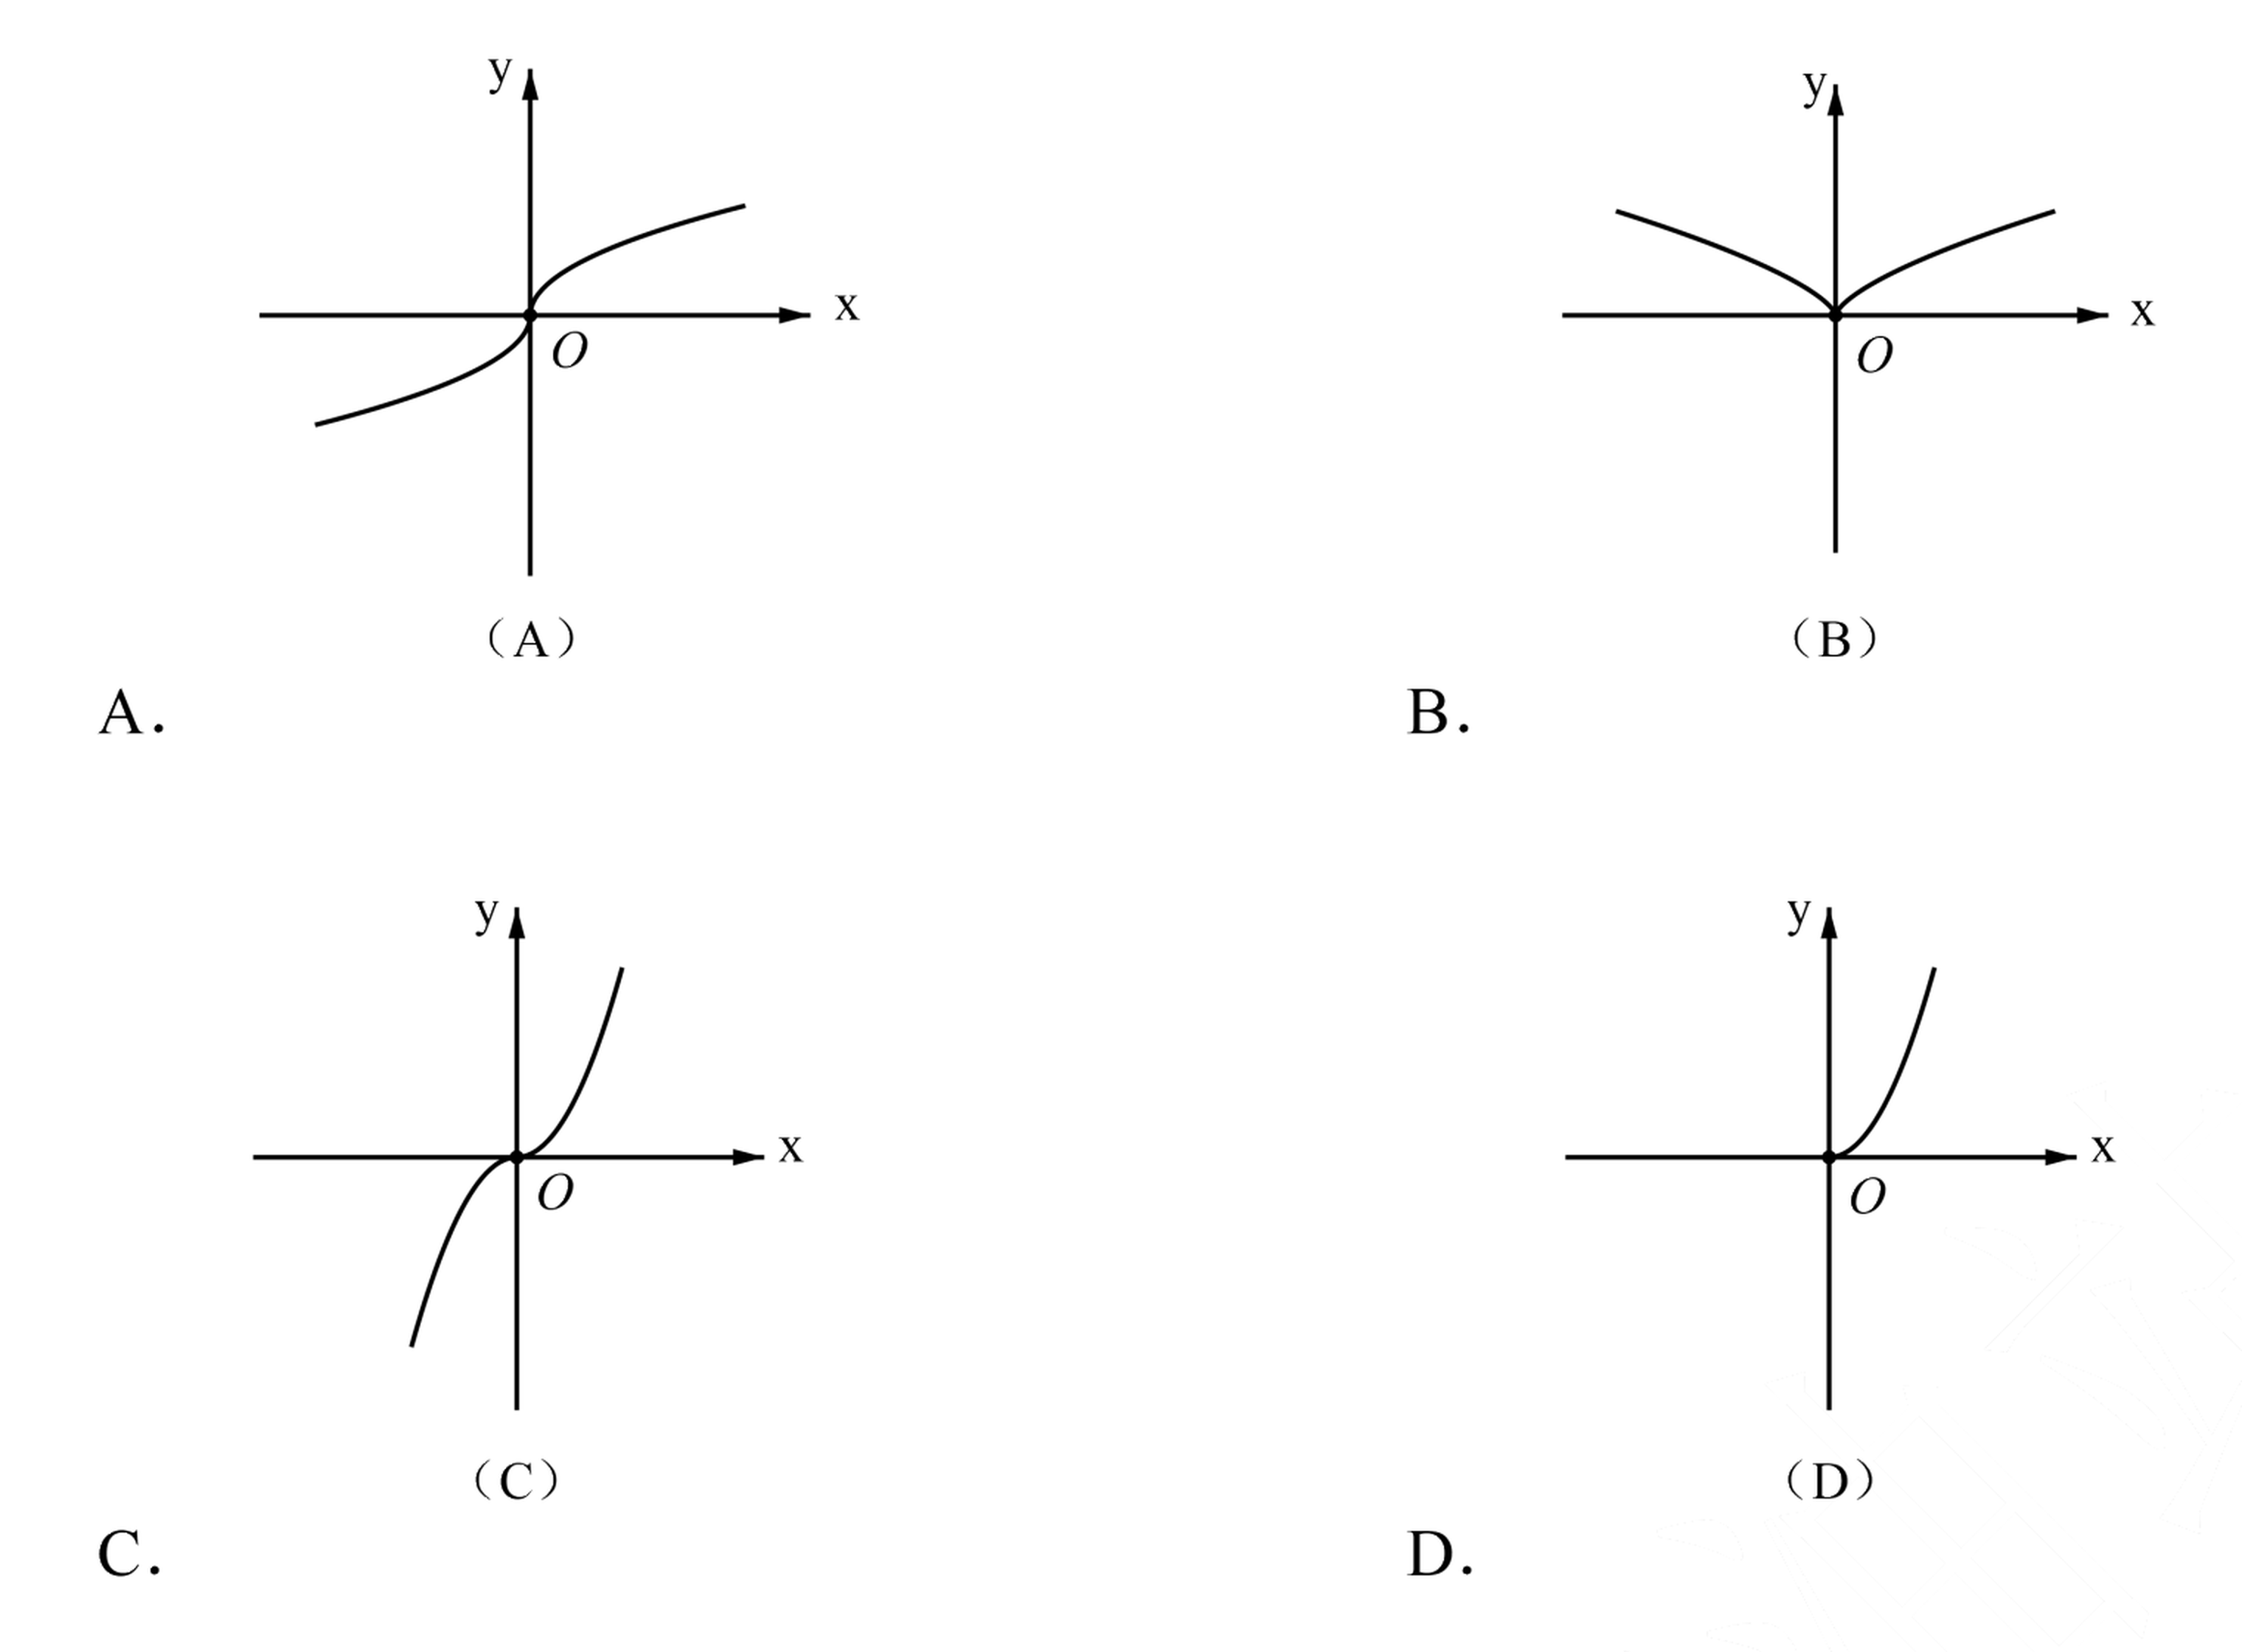
\includegraphics[width=0.80\textwidth]{figures/gao140_q14.png}
\end{center}

\ifanswer
\solbegin
\step{$f(x)=x^{\frac23}=\sqrt[3]{x^2}$ 是偶函数，且恒大于等于 $0$，故选 $B$.}
\solend
\fi

\item 设 $p$：关于 $x$ 的不等式 $x^2+ax+1>0$ 对 $x\in\R$ 恒成立，$q$：对数函数 $y=\log_{4-3a}x$ 在 $(0,+\infty)$ 上单调递减，那么 $p$ 是 $q$ 的\mbox{（\quad）}

\keepwithprev
A. 充分不必要条件\qquad B. 充要条件

C. 必要不充分条件\qquad D. 既不充分也不必要条件

\ifanswer
\solbegin
\step{$p\Leftrightarrow a^2-4<0\Leftrightarrow -2<a<2$. $q\Leftrightarrow 0<4-3a<1\Leftrightarrow 1<a<\dfrac43$.}
\step{由 $\left(1,\dfrac43\right)\subset(-2,2)$ 得 $q\Rightarrow p$；而 $a=0$ 时 $p$ 真、$q$ 假，}% 子集符号原卷印单线 $\subset$，照录
\step{故 $p$ 是 $q$ 的必要不充分条件，故选 $C$.}
\solend
\fi

\item “非空集合 $M$ 的元素都是集合 $P$ 的元素” 是假命题，现有下列命题：

(1) $M$ 的元素都不是 $P$ 的元素；(2) $M$ 中有不属于 $P$ 元素；% 原卷"不属于 P 元素"脱"的"字，照录

(3) $M$ 中有 $P$ 的元素；(4) $M$ 的元素不都是 $P$ 的元素，

其中真命题的个数是\mbox{（\quad）}

\keepwithprev
A. 1\qquad B. 2\qquad C. 3\qquad D. 4

\ifanswer
\solbegin
\step{由于 “非空集合 $M$ 的元素都是集合 $P$ 的元素” 是假命题，}
\step{得 “非空集合 $M$ 的元素至少有一个元素不属于集合 $P$” 是真命题.}
\step{则 (1) 不正确；(2) 正确；(3) $M$ 中不一定有 $P$ 的元素，例如 $M=\{a\}$，}
\step{则 $a\notin P$；(4) 正确.}
\step{综上，真命题只有 (2)(4). 故选 $B$.}
\solend
\fi

\end{enumerate}

\bigsec{三、解答题}

\begin{enumerate}
\setcounter{enumi}{16}

\item 设全集为 $\R$，集合 $A=\left\{x\mid\dfrac{2x}{x-1}\leqslant1\right\}$.

(1) 用区间表示集合 $A$；

(2) 若集合 $B=\{x\mid\lvert x+2\rvert+\lvert x-1\rvert=3\}$，求 $A\cup B$.

\ifanswer
\solbegin
\step{(1) 由 $\dfrac{2x}{x-1}\leqslant1\Leftrightarrow\dfrac{x+1}{x-1}\leqslant0$，故 $A=[-1,1)$，则 $\overline{A}=(-\infty,-1)\cup[1,+\infty)$；}
\step{(2) 由 $B=\{x\mid\lvert x+2\rvert+\lvert x-1\rvert=3\}=[-2,1]$，}
\step{结合上一问有 $A=[-1,1)$，所以 $A\cup B=B=[-2,1]$.}
\solend
\fi

\item (1) 已知指数函数 $y=a^x(a>0$ 且 $a\neq1)$ 在区间 $[-1,1]$ 上的最大值与最小值之和等于 $\dfrac52$，求实数 $a$ 的值.

(2) 已知幂函数 $y=x^{m^2+7m+10}(m\in\Z)$ 的图像关于 $y$ 轴对称，且在 $(0,+\infty)$ 上严格减. 若 $(a-1)^{m^2+7m+10}\geqslant(1+2a)^{m^2+7m+10}$. 求实数 $a$ 的取值范围.

\ifanswer
\solbegin
\step{(1) 指数函数 $y=a^x$ 在区间 $[-1,1]$ 上单调，所以 $a^1+a^{-1}=\dfrac52$，}
\step{所以 $a=2$ 或 $a=\dfrac12$；}
\step{(2) 由题意得 $m^2+7m+10<0$，所以 $-5<m<-2$，又因为 $m\in\Z$，}
\step{所以 $m=-4$ 或 $m=-3$，}
\step{当 $m=-4$ 时，$y=x^{m^2+7m+10}=x^{-2}$，为偶函数，}
\step{当 $m=-3$ 时，$y=x^{m^2+7m+10}=x^{-2}$，为偶函数，}
\step{所以 $m^2+7m+10=-2$，所以 $(a-1)^{-2}\geqslant(1+2a)^{-2}$，}
\step{所以 $\lvert a-1\rvert\leqslant\lvert 1+2a\rvert$，所以 $a\leqslant-2$ 或 $a\geqslant0$，所以 $a\in(-\infty,-2]\cup[0,+\infty)$.}
\solend
\fi

\item 设函数 $f(x)=ax^2+(1-a)x+a-2$ （$a\in\R$）.

(1) 若关于 $x$ 的不等式 $f(x)\leqslant0$ 的解集为 $\left[0,\dfrac12\right]$，求实数 $a$ 的值；

(2) 若 $a\geqslant0$，解关于 $x$ 的不等式：$f(x)<a-1$.

\ifanswer
\solbegin
\step{(1) 由解集得 $a>0$，且 $0$ 是方程 $f(x)=0$ 的根，故 $f(0)=a-2=0$，}
\step{得 $a=2$.}
\step{此时 $f(x)=2x^2-x=x(2x-1)$，$f(x)\leqslant0$ 的解集确为 $\left[0,\dfrac12\right]$.}
\step{(2) $f(x)<a-1\Leftrightarrow ax^2+(1-a)x-1<0\Leftrightarrow(x-1)(ax+1)<0$，}
\step{当 $a=0$ 时，$x-1<0$，解集为 $(-\infty,1)$.}
\step{当 $a>0$ 时，$-\dfrac1a<1$，解集为 $\left(-\dfrac1a,1\right)$.}
\solend
\fi

\item 为了保护环境，某单位采用新工艺，把二氧化碳转化为一种可利用的化工产品，已知该单位每月处理量最多不超过 $300$ 吨. 当月处理量为 $x$ 吨时，月处理成本为 $x^2-200x+40000(0<x\leqslant300)$ 元，且每处理一吨二氧化碳得到可利用的化工产品价值为 $300$ 元.

(1) 若要保证该单位每月不亏损，则每月处理量应控制在什么范围？

(2) 该单位每月处理量为多少吨时，才能使每吨的平均处理成本最低，最低为多少元？

\ifanswer
\solbegin
\step{(1) 由题意得 $S=300x-(x^2-200x+40000)$}
\step{$=-x^2+500x-40000(0<x\leqslant300)$，}
\step{令 $S\geqslant0$，即 $-x^2+500x-40000\geqslant0$，解得 $100\leqslant x\leqslant400$，}
\step{又 $0<x\leqslant300$，所以 $100\leqslant x\leqslant300$，}
\step{故要保证该单位每月不亏损，则每月处理量应控制在 $[100,300]$ 范围内；}
\step{(2) 每吨的平均出来成本为 $\dfrac yx=x+\dfrac{40000}x-200\geqslant2\sqrt{x\cdot\dfrac{40000}x}-200=200$，}% 原卷"平均出来成本"与题干"平均处理成本"措辞不一，照录
\step{当且仅当 $x=\dfrac{40000}x$，即 $x=200$ 时取等号，}
\step{所以该单位每月处理量为 $200$ 吨时，}
\step{才能使每吨的平均处理成本最低且最低为 $200$ 元.}
\solend
\fi

\item 已知函数 $y=f(x),x\in D$，若对于定义域 $D$ 内任意实数 $x,y$，不等式 $f(x)+f(y)\geqslant f(xy)$ 都成立，则称函数 $y=f(x)$ 是 $QB$ 函数，

(1) 判断函数 $f(x)=x+1$ 是否是 $QB$ 函数，并说明理由；

(2) 若函数 $g(x)=\ln(ax),x>0$ 是 $QB$ 函数，求实数 $a$ 的取值范围；

(3) 已知函数 $h(x)=a^x(a\in\R\text{ 且 }a>0)$，证明：“函数 $y=h(x)$ 是 $QB$ 函数” 的充要条件是 “ $a\in\{1\}$ ”.

\ifanswer
\solbegin
\step{(1) 不是，理由如下：因为 $f(x)=x+1$，}
\step{所以 $f(x)+f(y)\geqslant f(xy)\Leftrightarrow x+y\geqslant xy-1\Leftrightarrow(x-1)(y-1)\leqslant2$，}
\step{显然不恒成立，故不是 $QB$ 函数；}
\step{(2) 因为函数 $g(x)=\ln(ax),x>0$，则 $a>0$，}
\step{若函数 $g(x)$ 是 $QB$ 函数，则 $g(x)+g(y)\geqslant g(xy)$，}
\step{即 $\ln(ax)+\ln(ay)\geqslant\ln(axy)$，则 $\ln(a^2xy)\geqslant\ln(axy)$，得 $a^2xy\geqslant axy$，}
\step{且 $x>0,y>0$，得 $a^2\geqslant a$，解得 $a\geqslant1$ 或 $a\leqslant0$（舍去），}
\step{所以实数 $a$ 的取值范围为 $[1,+\infty)$.}
\step{(3) 若函数 $h(x)=a^x$ 是 $QB$ 函数，}
\step{当 $a>1$ 时，令 $x=y=\log_a\dfrac12$，则 $h(x)+h(y)=a^x+a^y=\dfrac12+\dfrac12=1$，}
\step{且 $h(xy)=a^{xy}=(a^x)^y=\left(\dfrac12\right)^{\log_a\frac12}=2^{\log_a2}$，}
\step{因为 $\log_a2>0$，所以 $h(xy)=2^{\log_a2}>1$，不满足 $h(x)+h(y)\geqslant h(xy)$，}
\step{不合题意；}
\step{当 $a=1$ 时，$h(x)+h(y)=a^x+a^y=1+1=2$，且 $h(xy)=a^{xy}=1$，}
\step{满足 $h(x)+h(y)\geqslant h(xy)$，符合题意；}
\step{当 $0<a<1$ 时，令 $x=\log_a2,y=2$，则 $h(x)+h(y)=a^x+a^y=2+a^2$，}
\step{且 $h(xy)=a^{xy}=(a^x)^y=2^2=4$，}
\step{因为 $0<a<1$，所以 $0<a^2<1$，得 $2<2+a^2<3$，}
\step{不满足 $h(x)+h(y)\geqslant h(xy)$，不合题意；}
\step{综上所述，$a\in\{1\}$，即充分性成立；}% 原卷"充分性/必要性"两标签与所证方向互换，照录
\step{若 $a\in\{1\}$，则 $h(x)+h(y)=a^x+a^y=1+1=2$，且 $h(xy)=a^{xy}=1$，}
\step{得 $h(x)+h(y)\geqslant h(xy)$，所以函数 $h(x)=a^x$ 是 $QB$ 函数，即必要性成立；}% 原卷"充分性/必要性"两标签与所证方向互换，照录
\step{综上所述，“函数 $y=h(x)$ 是 $QB$ 函数” 的充要条件是 “ $a\in\{1\}$ ”.}
\solend
\fi

\end{enumerate}

\end{document}
"
%
% ① 原始材料：微信公众号"魔都数学加油站"文章，连载"27学年高一140"，原文标题
% "27学年高一140——2026-2027年上海市甘泉外国语高一上期中"；
% 原文链接：https://mp.weixin.qq.com/s/eflgf2Ktk1LyT9x-k-ltLw。
% 正文为 9 张 PNG 页（01、02、03、05、06、07、08 为 4762x6735；04、09 为 2560x3620，
% 同一篇各页分辨率不同，逐页按各自分辨率裁图核对），题目下印有【答案】或【解析】，为讲评版。
% 题目、解析均据原图转录；卷面粉红色水印"魔都数学加油站"及公众号页脚未录入。
% 全卷 1 幅插图：第 14 题四幅坐标函数图象选项（04 页），取原卷截图去粉色水印、去色、
% LANCZOS 放大 2 倍，四幅选项按原卷 2x2 排布（含（A）（B）（C）（D）图注与 A./B./C./D.
% 选项字母）合并裁为一张；图前按惯例加 \needvspace 守卫。
%
% 卷首标题：原卷印作"2026-2027 年甘泉外国语高一上期中"（公众号标题中的"上海市"
% 卷面标题行没有，本稿照卷面），年份区间按全稿惯例排 en dash；原卷未印副标题，
% 本卷为期中卷、跨集合与常用逻辑用语／不等式／函数三章，按题目内容标为
% "集合与常用逻辑用语、不等式、函数"（与 125／126／128／129／131／132／133 同期中卷口径相同）：
% 集合与逻辑见 Q5、Q13、Q15、Q16、Q17，不等式见 Q3、Q10、Q11、Q19、Q20，
% 函数（指数／对数／幂函数及其图象、同构与 QB 函数）见 Q4、Q6、Q7、Q8、Q12、Q14、Q18、Q21。
%
% 题号体例：本卷共 19 题——一、填空题 3—12（10 题）、二、选择题 13—16（4 题）、
% 三、解答题 17—21（5 题）。三节分别 \setcounter{enumi}{2}／{12}／{16}。
% 原卷从第 3 题起、无第 1、2 题，本稿保留原题号。
%
% ② 与原卷的排版差异：
%   ① 原文从第 3 题起，本稿保留原题号；
%   ② 原卷每题下直接印【答案】或【解析】，本稿按全稿惯例置于答案版；第 5 题只印
%      【答案】、无【解析】，提 \ans{}；第 13、14、15、16 题答案均在【解析】末句
%      "故选 …"，题干括号内留空、不另提 \ans{}；其余各题印【解析】、无独立答案段；
%      全卷无"答案印在题干括号内且无解析"的一型；
%   ③ 原卷未印副标题，本稿按"知识模块"口径补出；
%   ④ 原卷填空横线按全稿惯例排为 \blankline[4.4em]；选择题括号排 \mbox{（\quad）}、
%      每个选项段前按惯例加 \keepwithprev（四幅图选项那一枚放在 \begin{center} 之前）；
%      解答题不留作答区、不加 \anspace（原卷为讲评版，与 129／131／132／133／136 同）；
%   ⑤ 原卷数集混排：斜体 $R$（Q9、Q12、Q15 等）与黑体／黑板粗体 $R$（Q15、Q17、
%      Q19、Q21）、粗体 $Z$（Q18），按全稿惯例统一改 \R／\Z；空集记号 \varnothing；
%      绝对值排 \lvert…\rvert，集合描述竖线排 \mid；不等号按全稿惯例排 \leqslant／\geqslant；
%      补集照原卷上划线排 \overline{A}；
%   ⑥ 子题标号 (1)(2)(3)(4) 原卷印半角括号，照录（与 131／132／133／134／136 同口径）；
%      括注原卷全角／半角混用，逐处照录：Q8"（结果用 a,b 表示）"、Q19"（a∈R）"、
%      Q21 (2)"（舍去）"印全角，Q18"$a^x(a>0$ 且 $a\neq1)$"、Q20"$40000(0<x\leqslant300)$"、
%      Q21 (3)"($a\in\R$ 且 $a>0$)"及 (0,+∞)、2(a>0) 等数学式内括注印半角；
%   ⑦ 数学式内半角逗号照录（如 Q8"$\lg2=a,10^b=3$"、Q11"$-2,3,4,\cdots,2027$"、
%      Q12"$x_1,x_2$"、Q19"$f(x)=ax^2+(1-a)x+a-2$"、Q21"$x>0,y>0$"）；
%      原卷行末西文句点照录（Q20 题干"300 吨. 当月处理量为 x 吨时"），行中全角逗号照录；
%   ⑧ 一幅插图：第 14 题四幅坐标函数图象选项合并裁为一张 \includegraphics
%      （题前 \needvspace{9cm}）。Q14 是"二、选择题"节内带大图块的第二题
%      （Q13 为节首题但无图），另在 \bigsec{二、选择题} 之前加 \needvspace{11cm}
%      连节标题一起量——守卫必须放在 \bigsec 之前，放标题之后会让"二、选择题"
%      孤立在页末（B 类，照 高一26／40／59／136 成例）；三版切页审计均"合计异常：无"；
%   ⑨ 跨页续印按题合并：Q9 题干在 01 页、解析续至 02 页；Q11 题干与解析前 3 行在 02 页、
%      后 2 行在 03 页；Q14 题干在 03 页末、四幅图与【解析】在 04 页；Q16 题干四条命题
%      在 04 页、选项与【解析】在 05 页；Q18 解析 (1) 首行在 05 页、其余 7 行在 06 页；
%      Q20 题干在 06 页末、"300 元."与两小问及【解析】在 07 页；Q21 解析跨 07—09 页
%      （末 3 行在 09 页）；本稿按题连排，不丢行；
%   ⑩ 题干中的中文弯引号按原卷照录，注释内一律 ASCII 引号；原卷"图像／图象"
%      两种写法混用，逐处照录（Q7、Q18 作"图像"，Q14 作"图象"）；
%   ⑪ 原卷无红色加粗标签（【解析】【答案】均黑色印刷），故本卷未用 \stepm。
%
% 判别式字形：全卷仅第 9 题【解析】"经验证得"cases 块出现两处判别式
%   "$\Delta=p^2-4q>0$"与"$\Delta'=q^2-4p>0$"，原卷两处均印等腰、偏高的
%   三角 $\Delta$（带撇的为 $\Delta'$），逐处放大核对并照录 \Delta、\Delta'；
%   全卷未出现扁等边三角 \triangle。
%
% 子集符号：第 15 题【解析】"由 (1,4/3)⊂(-2,2) 得 q⇒p"一处原卷印单线 $\subset$
%   （不带下划线），逐处放大核对、照录 \subset；全卷未出现带下划线的 \subseteq。
%
% 原卷存疑照录（均照录未改，正文对应处另有 % 注）：
%   第 16 题 (2) 命题"$M$ 中有不属于 $P$ 元素"中"不属于 $P$ 元素"脱"的"字，照录；
%   第 20 题题干 (2) 作"每吨的平均处理成本"、而【解析】(2) 作"每吨的平均出来成本"，
%      "出来"疑为"处理"之误，两处措辞照录不统一；
%   第 21 题 (3)【解析】"综上所述，$a\in\{1\}$，即充分性成立"与"即必要性成立"
%      两处标签与所证方向互换（按充要条件的通常口径），照录。
%
% 行数复核：一条 \step = 原卷解析的一个印刷行，cases 块作一个印刷行计。逐题数 \step
%   条数，合计 92 条（Q3：2；Q4：1；Q5：0；Q6：2；Q7：1；Q8：1；Q9：7；Q10：5；
%   Q11：5；Q12：4；Q13：6；Q14：1；Q15：3；Q16：5；Q17：3；Q18：8；Q19：6；
%   Q20：9；Q21：23），与原卷印刷行逐题相等。第 5 题只印【答案】、提 \ans{}，
%   不计入 \step 账；第 13、14、15、16 题答案在解析末句"故选 …"，括号内留空、
%   不另提 \ans{}；答案版【答案】/【解析】标记数 = 19（1 个 \ans + 18 个 \solbegin）
%   = 全卷题数。
%
\documentclass[a4paper,11pt]{article}
\usepackage{common}

\begin{document}

\examtitlest[3]{2026--2027 年甘泉外国语高一上期中}{集合与常用逻辑用语、不等式、函数}

\bigsec{一、填空题}

\begin{enumerate}
\setcounter{enumi}{2}

\item 不等式 $x^2-2x-3<0$ 的解集为\blankline[4.4em].

\ifanswer
\solbegin
\step{方程 $x^2-2x-3=0$ 的实数根是 $x_1=-1$，$x_2=3$；}
\step{所以不等式 $x^2-2x-3<0$ 的解集为 $\{x\mid -1<x<3\}$.}
\solend
\fi

\item 根式 $\sqrt{x\sqrt{x}}(x>0)$ 的指数幂形式为\blankline[4.4em].

\ifanswer
\solbegin
\step{$\sqrt{x\sqrt{x}}=\sqrt{x\cdot x^{\frac12}}=\sqrt{x^{\frac32}}=x^{\frac34}$.}
\solend
\fi

\item 陈述句 “ $x>1$ 或 $y>1$ ” 的否定形式是\blankline[4.4em].

\ifanswer
\ans{$x\leqslant1$ 且 $y\leqslant1$}
\fi

\item 若 $x<0$ 时，指数函数 $y=(a-1)^x$ 的值总大于 $1$，则实数 $a$ 的取值范围是\blankline[4.4em].

\ifanswer
\solbegin
\step{由题意得 $(a-1)^x>1$ 在 $(-\infty,0)$ 上恒成立，则 $0<a-1<1$，解得 $1<a<2$.}
\step{故实数 $a$ 的取值范围是 $(1,2)$.}
\solend
\fi

\item 若 $f(x)=\log_a(x-1)$，对任意 $a>0$ 且 $a\neq1$，函数 $y=f(x)$ 的图像必过定点\blankline[4.4em].

\ifanswer
\solbegin
\step{令 $x-1=1$，即 $x=2$，此时 $f(2)=0$，即函数图像过定点 $(2,0)$.}
\solend
\fi

\item 已知 $\lg 2=a,10^b=3$，则 $\log_6 2=$\blankline[4.4em]（结果用 $a,b$ 表示）.

\ifanswer
\solbegin
\step{由 $10^b=3$，得 $b=\lg 3$，则 $\log_6 2=\dfrac{\lg 2}{\lg 6}=\dfrac{\lg 2}{\lg 2+\lg 3}=\dfrac{a}{a+b}$.}
\solend
\fi

\item 已知 $p$、$q\in\R$，$x_1$、$x_2$ 是关于 $x$ 的方程 $x^2+px+q=0$ 的两实根，$x_1+1$、$x_2+1$ 是关于 $x$ 的方程 $x^2+qx+p=0$ 的两实根，则 $pq=$\blankline[4.4em].

\ifanswer
\solbegin
\step{因为 $x_1$、$x_2$ 是关于 $x$ 的方程 $x^2+px+q=0$ 的两实根，}
\step{由韦达定理得 $x_1+x_2=-p$，$x_1\cdot x_2=q$，}
\step{因为 $x_1+1$、$x_2+1$ 是关于 $x$ 的方程 $x^2+qx+p=0$ 的两实根，}
\step{由韦达定理得 $x_1+1+x_2+1=-q$，$(x_1+1)(x_2+1)=p$，}
\step{即 $x_1+x_2=-q-2$，$x_1+x_2+x_1x_2=p-1$，又 $x_1+x_2=-p$，$x_1\cdot x_2=q$，}
\step{所以 $\begin{cases}-p=-q-2\\-p+q=p-1\end{cases}$，解得 $\begin{cases}p=-1\\q=-3\end{cases}$，经验证得 $\begin{cases}\Delta=p^2-4q>0\\\Delta'=q^2-4p>0\end{cases}$，}% 判别式原卷印高三角 $\Delta$、$\Delta'$，照录
\step{则 $pq=3$.}
\solend
\fi

\item 对于 $x\in\R$，不等式 $\lvert 3-x\rvert+\lvert 1+x\rvert\geqslant a^2-3a$ 恒成立，则实数 $a$ 的取值范围是\blankline[4.4em].

\ifanswer
\solbegin
\step{对于 $x\in\R$，不等式 $\lvert 3-x\rvert+\lvert 1+x\rvert\geqslant a^2-3a$ 恒成立，}
\step{即 $\lvert 3-x\rvert+\lvert 1+x\rvert$ 的最小值大于或等于 $a^2-3a$，}
\step{$\lvert 3-x\rvert+\lvert 1+x\rvert$ 表示数轴上的 $x$ 对应点到 $3$ 和 $-1$ 对应点的距离之和，}
\step{它的最小值为 $4$，故 $4\geqslant a^2-3a$，即 $a^2-3a-4\leqslant0$，解得 $-1\leqslant a\leqslant4$，}
\step{故实数 $a$ 的取值范围是 $[-1,4]$.}
\solend
\fi

\item 已知同时满足不等式 $x^2-x-2>0$ 和 $2x^2+(5+2a)x+5a<0$ 的 $x$ 的整数值只有 $2026$ 个，则实数 $a$ 的取值范围是\blankline[4.4em].

\ifanswer
\solbegin
\step{整数 $x$ 须满足 $x\leqslant-2$ 或 $x\geqslant3$，且 $(2x+5)(x+a)<0$.}
\step{当 $a<\dfrac52$ 时，需使整数解恰为 $-2,3,4,\cdots,2027$，即 $2027<-a\leqslant2028$.}
\step{当 $a>\dfrac52$ 时，需使整数解恰为 $-2028,-2027,\cdots,-3$，即 $2028<a\leqslant2029$；}
\step{$a=\dfrac52$ 时无解.}
\step{故 $a\in[-2028,-2027)\cup(2028,2029]$.}
\solend
\fi

\item 同构式通俗讲是结构相同的表达式，如：$f(x)=x+e^x$，$f(\ln x)=\ln x+e^{\ln x}=\ln x+x$，称 $x+e^x$ 与 $\ln x+x$ 为同构式. 已知实数 $x_1,x_2$ 满足 $e^{x_1}+x_1=8,\ln\sqrt[5]{5x_2+3}+x_2=1$，则 $x_1+5x_2=$\blankline[4.4em].

\ifanswer
\solbegin
\step{函数 $f(x)=x+e^x$ 在 $\R$ 上严格增，且 $f(x_1)=x_1+e^{x_1}=8$，}
\step{由 $\ln\sqrt[5]{5x_2+3}+x_2=1$，得 $\ln(5x_2+3)+5x_2=5$，则 $\ln(5x_2+3)+5x_2+3=8$，}
\step{即 $f(\ln(5x_2+3))=8$，因此 $f(\ln(5x_2+3))=8=f(x_1)$，则 $x_1=\ln(5x_2+3)$，}
\step{所以 $x_1+5x_2=\ln(5x_2+3)+5x_2=5$.}
\solend
\fi

\end{enumerate}

% 第 14 题四幅图是"二、选择题"节内的大图块；守卫须放在 \bigsec 之前连节标题一起量，
% 否则"二、选择题"会孤立在页末（B 类，照 高一26／40／59／136 成例）
\needvspace{11cm}
\bigsec{二、选择题}

\begin{enumerate}
\setcounter{enumi}{12}

\item 设 $a$、$b$ 为实数，则 “ $a>b>0$ ” 的一个充分非必要条件是\mbox{（\quad）}

\keepwithprev
A. $\sqrt{a-1}>\sqrt{b-1}$\qquad B. $a^2>b^2$

C. $\dfrac1b>\dfrac1a$\qquad D. $a-b>b-a$

\ifanswer
\solbegin
\step{由 $\sqrt{a-1}>\sqrt{b-1}$ 得 $a>b\geqslant1$，故 $a>b>0$，反之不成立，满足题意；}
\step{由 $a^2>b^2$，则 $\lvert a\rvert>\lvert b\rvert$，推不出 $a>b>0$，反向可推出，不满足；}
\step{由 $\dfrac1b>\dfrac1a$，则 $a>b>0$ 或 $b>0>a$ 或 $0>a>b$，推不出 $a>b>0$，}
\step{反向可推出，不满足；}
\step{由 $a-b>b-a$，则 $a>b$，推不出 $a>b>0$，反向可推出，不满足；}
\step{故选 $A$.}
\solend
\fi

% 第 14 题四幅坐标函数图象选项是一整块，守卫放在 \item 之前
\needvspace{9cm}
\item 幂函数 $f(x)=x^{\frac23}$ 的图象大致为\mbox{（\quad）}

\keepwithprev
\begin{center}
% 四幅坐标函数图象选项取原卷 04 页截图去粉色水印、去色，按原卷 2x2 排布合并为一张
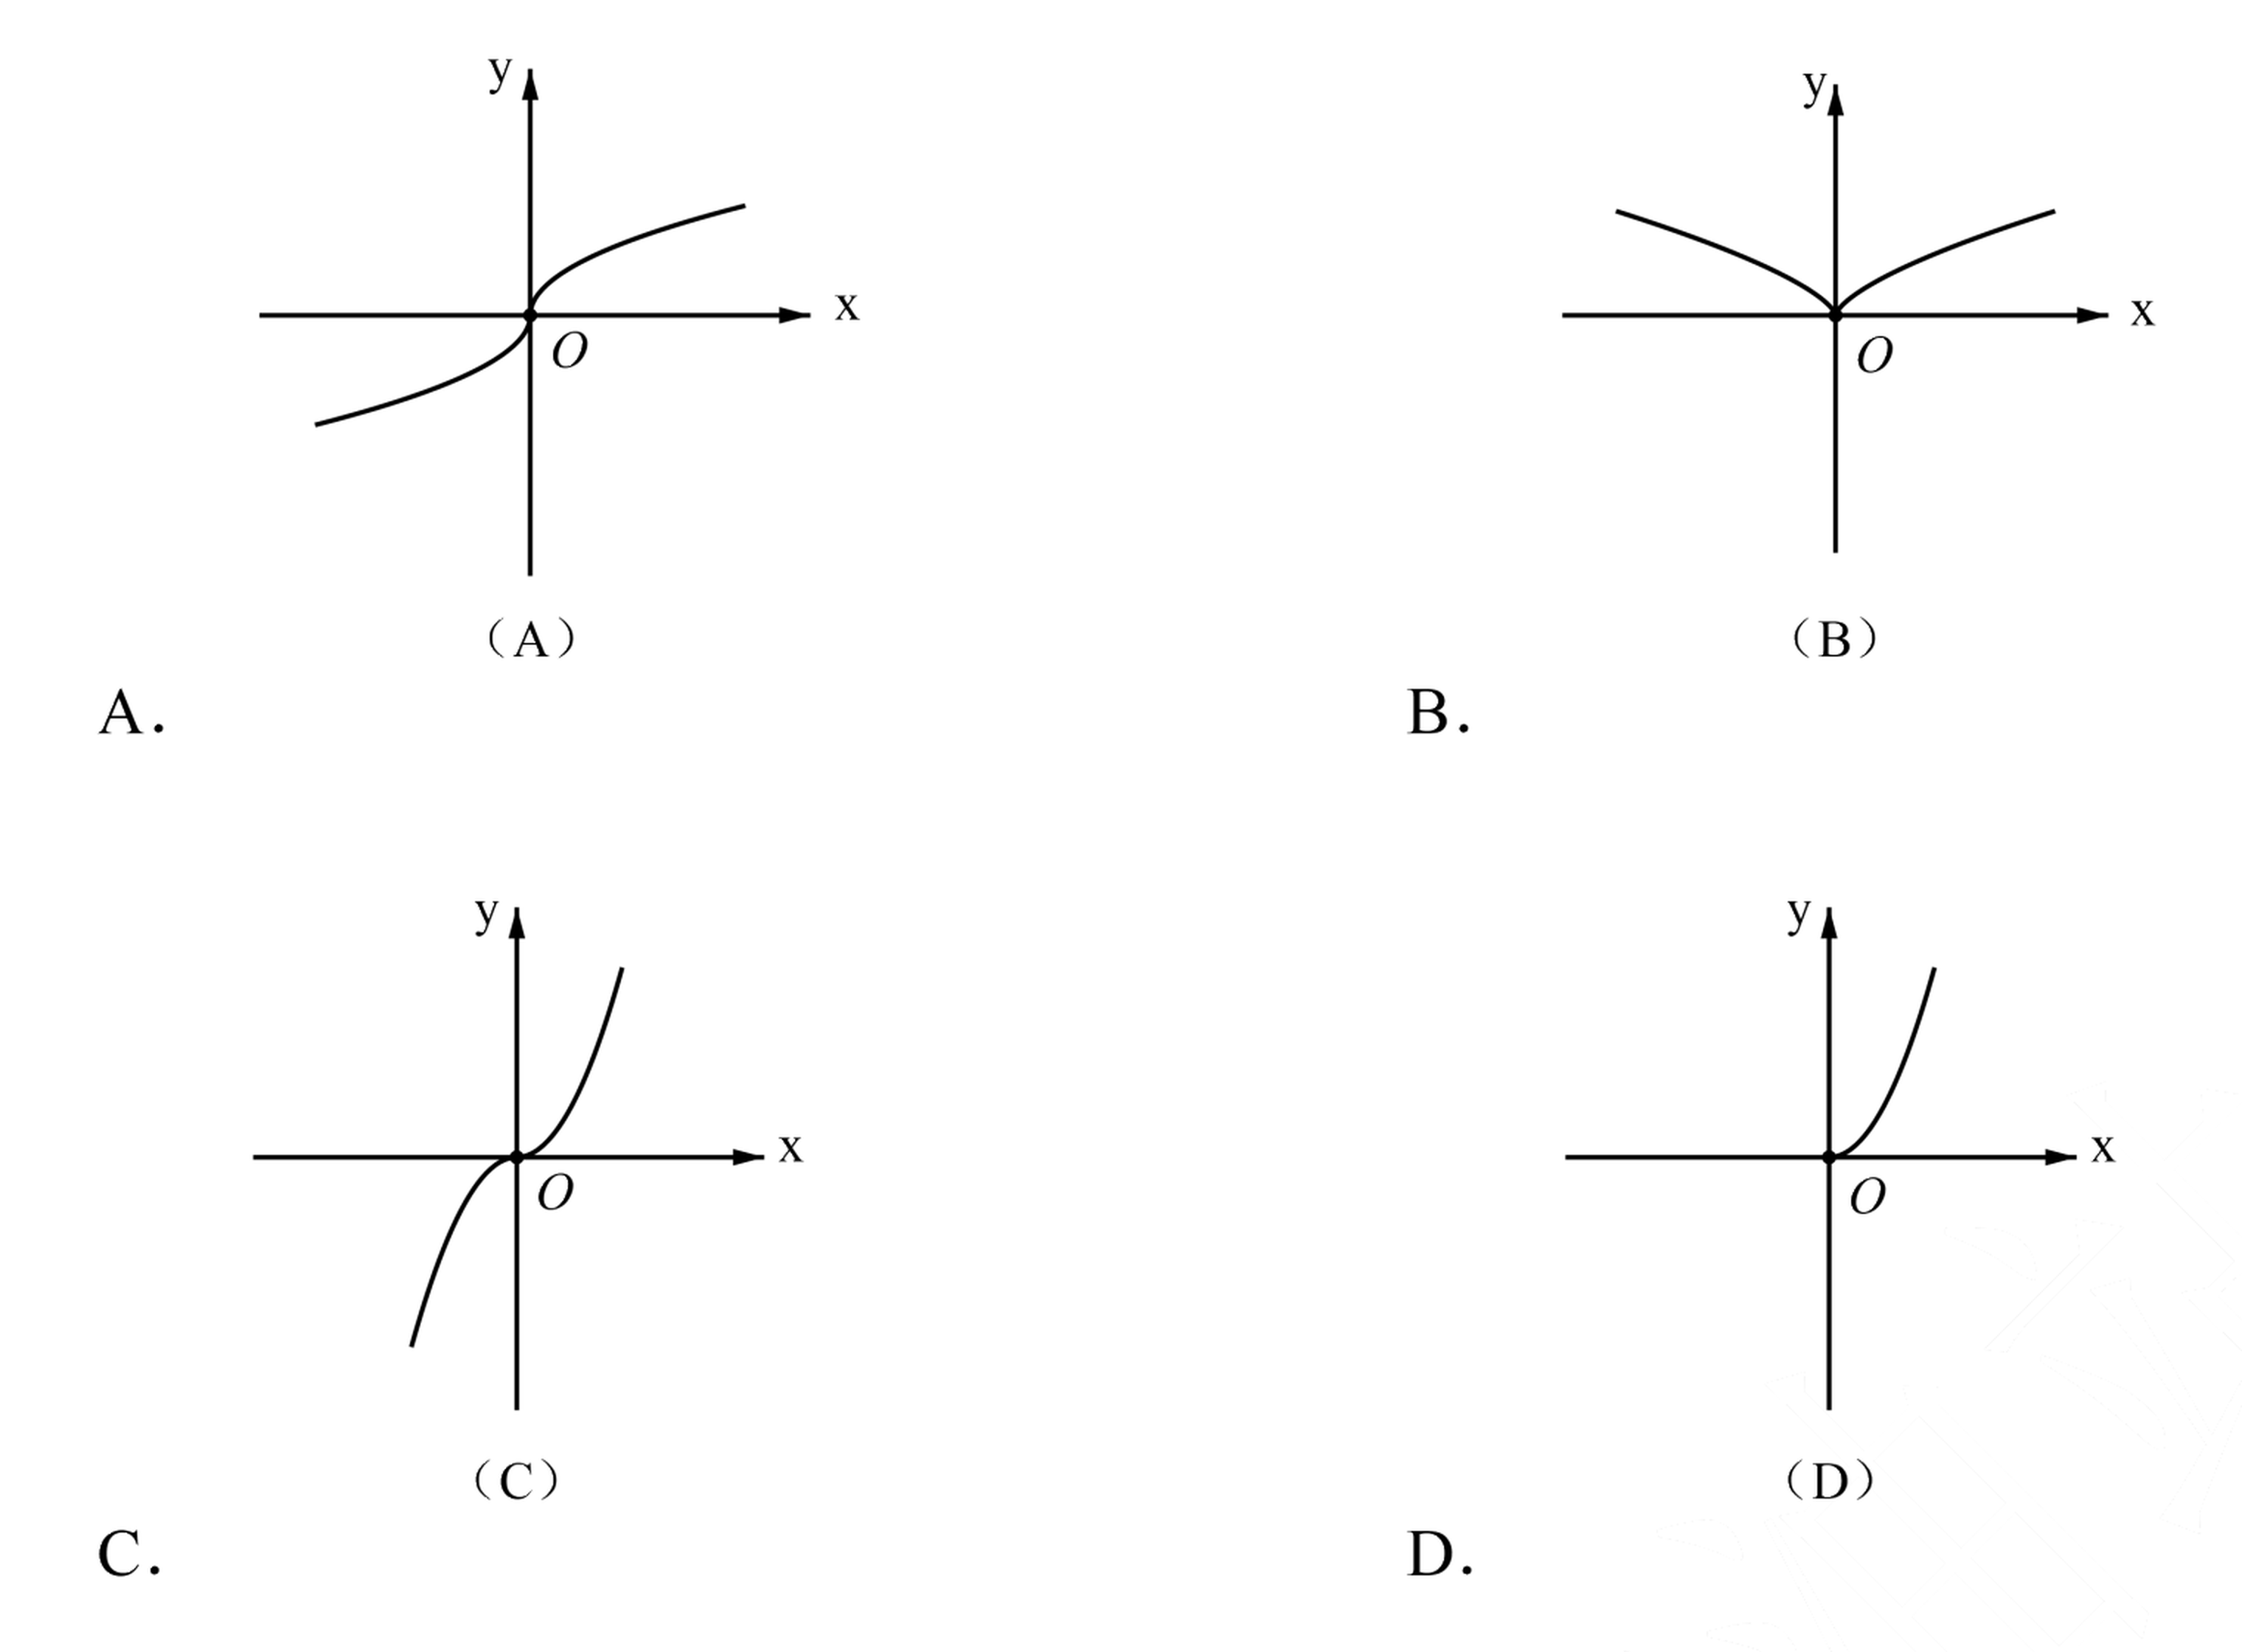
\includegraphics[width=0.80\textwidth]{figures/gao140_q14.png}
\end{center}

\ifanswer
\solbegin
\step{$f(x)=x^{\frac23}=\sqrt[3]{x^2}$ 是偶函数，且恒大于等于 $0$，故选 $B$.}
\solend
\fi

\item 设 $p$：关于 $x$ 的不等式 $x^2+ax+1>0$ 对 $x\in\R$ 恒成立，$q$：对数函数 $y=\log_{4-3a}x$ 在 $(0,+\infty)$ 上单调递减，那么 $p$ 是 $q$ 的\mbox{（\quad）}

\keepwithprev
A. 充分不必要条件\qquad B. 充要条件

C. 必要不充分条件\qquad D. 既不充分也不必要条件

\ifanswer
\solbegin
\step{$p\Leftrightarrow a^2-4<0\Leftrightarrow -2<a<2$. $q\Leftrightarrow 0<4-3a<1\Leftrightarrow 1<a<\dfrac43$.}
\step{由 $\left(1,\dfrac43\right)\subset(-2,2)$ 得 $q\Rightarrow p$；而 $a=0$ 时 $p$ 真、$q$ 假，}% 子集符号原卷印单线 $\subset$，照录
\step{故 $p$ 是 $q$ 的必要不充分条件，故选 $C$.}
\solend
\fi

\item “非空集合 $M$ 的元素都是集合 $P$ 的元素” 是假命题，现有下列命题：

(1) $M$ 的元素都不是 $P$ 的元素；(2) $M$ 中有不属于 $P$ 元素；% 原卷"不属于 P 元素"脱"的"字，照录

(3) $M$ 中有 $P$ 的元素；(4) $M$ 的元素不都是 $P$ 的元素，

其中真命题的个数是\mbox{（\quad）}

\keepwithprev
A. 1\qquad B. 2\qquad C. 3\qquad D. 4

\ifanswer
\solbegin
\step{由于 “非空集合 $M$ 的元素都是集合 $P$ 的元素” 是假命题，}
\step{得 “非空集合 $M$ 的元素至少有一个元素不属于集合 $P$” 是真命题.}
\step{则 (1) 不正确；(2) 正确；(3) $M$ 中不一定有 $P$ 的元素，例如 $M=\{a\}$，}
\step{则 $a\notin P$；(4) 正确.}
\step{综上，真命题只有 (2)(4). 故选 $B$.}
\solend
\fi

\end{enumerate}

\bigsec{三、解答题}

\begin{enumerate}
\setcounter{enumi}{16}

\item 设全集为 $\R$，集合 $A=\left\{x\mid\dfrac{2x}{x-1}\leqslant1\right\}$.

(1) 用区间表示集合 $A$；

(2) 若集合 $B=\{x\mid\lvert x+2\rvert+\lvert x-1\rvert=3\}$，求 $A\cup B$.

\ifanswer
\solbegin
\step{(1) 由 $\dfrac{2x}{x-1}\leqslant1\Leftrightarrow\dfrac{x+1}{x-1}\leqslant0$，故 $A=[-1,1)$，则 $\overline{A}=(-\infty,-1)\cup[1,+\infty)$；}
\step{(2) 由 $B=\{x\mid\lvert x+2\rvert+\lvert x-1\rvert=3\}=[-2,1]$，}
\step{结合上一问有 $A=[-1,1)$，所以 $A\cup B=B=[-2,1]$.}
\solend
\fi

\item (1) 已知指数函数 $y=a^x(a>0$ 且 $a\neq1)$ 在区间 $[-1,1]$ 上的最大值与最小值之和等于 $\dfrac52$，求实数 $a$ 的值.

(2) 已知幂函数 $y=x^{m^2+7m+10}(m\in\Z)$ 的图像关于 $y$ 轴对称，且在 $(0,+\infty)$ 上严格减. 若 $(a-1)^{m^2+7m+10}\geqslant(1+2a)^{m^2+7m+10}$. 求实数 $a$ 的取值范围.

\ifanswer
\solbegin
\step{(1) 指数函数 $y=a^x$ 在区间 $[-1,1]$ 上单调，所以 $a^1+a^{-1}=\dfrac52$，}
\step{所以 $a=2$ 或 $a=\dfrac12$；}
\step{(2) 由题意得 $m^2+7m+10<0$，所以 $-5<m<-2$，又因为 $m\in\Z$，}
\step{所以 $m=-4$ 或 $m=-3$，}
\step{当 $m=-4$ 时，$y=x^{m^2+7m+10}=x^{-2}$，为偶函数，}
\step{当 $m=-3$ 时，$y=x^{m^2+7m+10}=x^{-2}$，为偶函数，}
\step{所以 $m^2+7m+10=-2$，所以 $(a-1)^{-2}\geqslant(1+2a)^{-2}$，}
\step{所以 $\lvert a-1\rvert\leqslant\lvert 1+2a\rvert$，所以 $a\leqslant-2$ 或 $a\geqslant0$，所以 $a\in(-\infty,-2]\cup[0,+\infty)$.}
\solend
\fi

\item 设函数 $f(x)=ax^2+(1-a)x+a-2$ （$a\in\R$）.

(1) 若关于 $x$ 的不等式 $f(x)\leqslant0$ 的解集为 $\left[0,\dfrac12\right]$，求实数 $a$ 的值；

(2) 若 $a\geqslant0$，解关于 $x$ 的不等式：$f(x)<a-1$.

\ifanswer
\solbegin
\step{(1) 由解集得 $a>0$，且 $0$ 是方程 $f(x)=0$ 的根，故 $f(0)=a-2=0$，}
\step{得 $a=2$.}
\step{此时 $f(x)=2x^2-x=x(2x-1)$，$f(x)\leqslant0$ 的解集确为 $\left[0,\dfrac12\right]$.}
\step{(2) $f(x)<a-1\Leftrightarrow ax^2+(1-a)x-1<0\Leftrightarrow(x-1)(ax+1)<0$，}
\step{当 $a=0$ 时，$x-1<0$，解集为 $(-\infty,1)$.}
\step{当 $a>0$ 时，$-\dfrac1a<1$，解集为 $\left(-\dfrac1a,1\right)$.}
\solend
\fi

\item 为了保护环境，某单位采用新工艺，把二氧化碳转化为一种可利用的化工产品，已知该单位每月处理量最多不超过 $300$ 吨. 当月处理量为 $x$ 吨时，月处理成本为 $x^2-200x+40000(0<x\leqslant300)$ 元，且每处理一吨二氧化碳得到可利用的化工产品价值为 $300$ 元.

(1) 若要保证该单位每月不亏损，则每月处理量应控制在什么范围？

(2) 该单位每月处理量为多少吨时，才能使每吨的平均处理成本最低，最低为多少元？

\ifanswer
\solbegin
\step{(1) 由题意得 $S=300x-(x^2-200x+40000)$}
\step{$=-x^2+500x-40000(0<x\leqslant300)$，}
\step{令 $S\geqslant0$，即 $-x^2+500x-40000\geqslant0$，解得 $100\leqslant x\leqslant400$，}
\step{又 $0<x\leqslant300$，所以 $100\leqslant x\leqslant300$，}
\step{故要保证该单位每月不亏损，则每月处理量应控制在 $[100,300]$ 范围内；}
\step{(2) 每吨的平均出来成本为 $\dfrac yx=x+\dfrac{40000}x-200\geqslant2\sqrt{x\cdot\dfrac{40000}x}-200=200$，}% 原卷"平均出来成本"与题干"平均处理成本"措辞不一，照录
\step{当且仅当 $x=\dfrac{40000}x$，即 $x=200$ 时取等号，}
\step{所以该单位每月处理量为 $200$ 吨时，}
\step{才能使每吨的平均处理成本最低且最低为 $200$ 元.}
\solend
\fi

\item 已知函数 $y=f(x),x\in D$，若对于定义域 $D$ 内任意实数 $x,y$，不等式 $f(x)+f(y)\geqslant f(xy)$ 都成立，则称函数 $y=f(x)$ 是 $QB$ 函数，

(1) 判断函数 $f(x)=x+1$ 是否是 $QB$ 函数，并说明理由；

(2) 若函数 $g(x)=\ln(ax),x>0$ 是 $QB$ 函数，求实数 $a$ 的取值范围；

(3) 已知函数 $h(x)=a^x(a\in\R\text{ 且 }a>0)$，证明：“函数 $y=h(x)$ 是 $QB$ 函数” 的充要条件是 “ $a\in\{1\}$ ”.

\ifanswer
\solbegin
\step{(1) 不是，理由如下：因为 $f(x)=x+1$，}
\step{所以 $f(x)+f(y)\geqslant f(xy)\Leftrightarrow x+y\geqslant xy-1\Leftrightarrow(x-1)(y-1)\leqslant2$，}
\step{显然不恒成立，故不是 $QB$ 函数；}
\step{(2) 因为函数 $g(x)=\ln(ax),x>0$，则 $a>0$，}
\step{若函数 $g(x)$ 是 $QB$ 函数，则 $g(x)+g(y)\geqslant g(xy)$，}
\step{即 $\ln(ax)+\ln(ay)\geqslant\ln(axy)$，则 $\ln(a^2xy)\geqslant\ln(axy)$，得 $a^2xy\geqslant axy$，}
\step{且 $x>0,y>0$，得 $a^2\geqslant a$，解得 $a\geqslant1$ 或 $a\leqslant0$（舍去），}
\step{所以实数 $a$ 的取值范围为 $[1,+\infty)$.}
\step{(3) 若函数 $h(x)=a^x$ 是 $QB$ 函数，}
\step{当 $a>1$ 时，令 $x=y=\log_a\dfrac12$，则 $h(x)+h(y)=a^x+a^y=\dfrac12+\dfrac12=1$，}
\step{且 $h(xy)=a^{xy}=(a^x)^y=\left(\dfrac12\right)^{\log_a\frac12}=2^{\log_a2}$，}
\step{因为 $\log_a2>0$，所以 $h(xy)=2^{\log_a2}>1$，不满足 $h(x)+h(y)\geqslant h(xy)$，}
\step{不合题意；}
\step{当 $a=1$ 时，$h(x)+h(y)=a^x+a^y=1+1=2$，且 $h(xy)=a^{xy}=1$，}
\step{满足 $h(x)+h(y)\geqslant h(xy)$，符合题意；}
\step{当 $0<a<1$ 时，令 $x=\log_a2,y=2$，则 $h(x)+h(y)=a^x+a^y=2+a^2$，}
\step{且 $h(xy)=a^{xy}=(a^x)^y=2^2=4$，}
\step{因为 $0<a<1$，所以 $0<a^2<1$，得 $2<2+a^2<3$，}
\step{不满足 $h(x)+h(y)\geqslant h(xy)$，不合题意；}
\step{综上所述，$a\in\{1\}$，即充分性成立；}% 原卷"充分性/必要性"两标签与所证方向互换，照录
\step{若 $a\in\{1\}$，则 $h(x)+h(y)=a^x+a^y=1+1=2$，且 $h(xy)=a^{xy}=1$，}
\step{得 $h(x)+h(y)\geqslant h(xy)$，所以函数 $h(x)=a^x$ 是 $QB$ 函数，即必要性成立；}% 原卷"充分性/必要性"两标签与所证方向互换，照录
\step{综上所述，“函数 $y=h(x)$ 是 $QB$ 函数” 的充要条件是 “ $a\in\{1\}$ ”.}
\solend
\fi

\end{enumerate}

\end{document}
"
% 紧凑版：xelatex "\def\iscompact{1}% 高一140_甘泉外国语_期中.tex
%   —— 高一上数学"2026-2027 年甘泉外国语高一上期中"（试卷版/答案版）
% 试卷版：xelatex 高一140_甘泉外国语_期中.tex
% 答案版：xelatex "\def\isanswer{1}% 高一140_甘泉外国语_期中.tex
%   —— 高一上数学"2026-2027 年甘泉外国语高一上期中"（试卷版/答案版）
% 试卷版：xelatex 高一140_甘泉外国语_期中.tex
% 答案版：xelatex "\def\isanswer{1}\input{高一140_甘泉外国语_期中.tex}"
% 紧凑版：xelatex "\def\iscompact{1}\input{高一140_甘泉外国语_期中.tex}"
%
% ① 原始材料：微信公众号"魔都数学加油站"文章，连载"27学年高一140"，原文标题
% "27学年高一140——2026-2027年上海市甘泉外国语高一上期中"；
% 原文链接：https://mp.weixin.qq.com/s/eflgf2Ktk1LyT9x-k-ltLw。
% 正文为 9 张 PNG 页（01、02、03、05、06、07、08 为 4762x6735；04、09 为 2560x3620，
% 同一篇各页分辨率不同，逐页按各自分辨率裁图核对），题目下印有【答案】或【解析】，为讲评版。
% 题目、解析均据原图转录；卷面粉红色水印"魔都数学加油站"及公众号页脚未录入。
% 全卷 1 幅插图：第 14 题四幅坐标函数图象选项（04 页），取原卷截图去粉色水印、去色、
% LANCZOS 放大 2 倍，四幅选项按原卷 2x2 排布（含（A）（B）（C）（D）图注与 A./B./C./D.
% 选项字母）合并裁为一张；图前按惯例加 \needvspace 守卫。
%
% 卷首标题：原卷印作"2026-2027 年甘泉外国语高一上期中"（公众号标题中的"上海市"
% 卷面标题行没有，本稿照卷面），年份区间按全稿惯例排 en dash；原卷未印副标题，
% 本卷为期中卷、跨集合与常用逻辑用语／不等式／函数三章，按题目内容标为
% "集合与常用逻辑用语、不等式、函数"（与 125／126／128／129／131／132／133 同期中卷口径相同）：
% 集合与逻辑见 Q5、Q13、Q15、Q16、Q17，不等式见 Q3、Q10、Q11、Q19、Q20，
% 函数（指数／对数／幂函数及其图象、同构与 QB 函数）见 Q4、Q6、Q7、Q8、Q12、Q14、Q18、Q21。
%
% 题号体例：本卷共 19 题——一、填空题 3—12（10 题）、二、选择题 13—16（4 题）、
% 三、解答题 17—21（5 题）。三节分别 \setcounter{enumi}{2}／{12}／{16}。
% 原卷从第 3 题起、无第 1、2 题，本稿保留原题号。
%
% ② 与原卷的排版差异：
%   ① 原文从第 3 题起，本稿保留原题号；
%   ② 原卷每题下直接印【答案】或【解析】，本稿按全稿惯例置于答案版；第 5 题只印
%      【答案】、无【解析】，提 \ans{}；第 13、14、15、16 题答案均在【解析】末句
%      "故选 …"，题干括号内留空、不另提 \ans{}；其余各题印【解析】、无独立答案段；
%      全卷无"答案印在题干括号内且无解析"的一型；
%   ③ 原卷未印副标题，本稿按"知识模块"口径补出；
%   ④ 原卷填空横线按全稿惯例排为 \blankline[4.4em]；选择题括号排 \mbox{（\quad）}、
%      每个选项段前按惯例加 \keepwithprev（四幅图选项那一枚放在 \begin{center} 之前）；
%      解答题不留作答区、不加 \anspace（原卷为讲评版，与 129／131／132／133／136 同）；
%   ⑤ 原卷数集混排：斜体 $R$（Q9、Q12、Q15 等）与黑体／黑板粗体 $R$（Q15、Q17、
%      Q19、Q21）、粗体 $Z$（Q18），按全稿惯例统一改 \R／\Z；空集记号 \varnothing；
%      绝对值排 \lvert…\rvert，集合描述竖线排 \mid；不等号按全稿惯例排 \leqslant／\geqslant；
%      补集照原卷上划线排 \overline{A}；
%   ⑥ 子题标号 (1)(2)(3)(4) 原卷印半角括号，照录（与 131／132／133／134／136 同口径）；
%      括注原卷全角／半角混用，逐处照录：Q8"（结果用 a,b 表示）"、Q19"（a∈R）"、
%      Q21 (2)"（舍去）"印全角，Q18"$a^x(a>0$ 且 $a\neq1)$"、Q20"$40000(0<x\leqslant300)$"、
%      Q21 (3)"($a\in\R$ 且 $a>0$)"及 (0,+∞)、2(a>0) 等数学式内括注印半角；
%   ⑦ 数学式内半角逗号照录（如 Q8"$\lg2=a,10^b=3$"、Q11"$-2,3,4,\cdots,2027$"、
%      Q12"$x_1,x_2$"、Q19"$f(x)=ax^2+(1-a)x+a-2$"、Q21"$x>0,y>0$"）；
%      原卷行末西文句点照录（Q20 题干"300 吨. 当月处理量为 x 吨时"），行中全角逗号照录；
%   ⑧ 一幅插图：第 14 题四幅坐标函数图象选项合并裁为一张 \includegraphics
%      （题前 \needvspace{9cm}）。Q14 是"二、选择题"节内带大图块的第二题
%      （Q13 为节首题但无图），另在 \bigsec{二、选择题} 之前加 \needvspace{11cm}
%      连节标题一起量——守卫必须放在 \bigsec 之前，放标题之后会让"二、选择题"
%      孤立在页末（B 类，照 高一26／40／59／136 成例）；三版切页审计均"合计异常：无"；
%   ⑨ 跨页续印按题合并：Q9 题干在 01 页、解析续至 02 页；Q11 题干与解析前 3 行在 02 页、
%      后 2 行在 03 页；Q14 题干在 03 页末、四幅图与【解析】在 04 页；Q16 题干四条命题
%      在 04 页、选项与【解析】在 05 页；Q18 解析 (1) 首行在 05 页、其余 7 行在 06 页；
%      Q20 题干在 06 页末、"300 元."与两小问及【解析】在 07 页；Q21 解析跨 07—09 页
%      （末 3 行在 09 页）；本稿按题连排，不丢行；
%   ⑩ 题干中的中文弯引号按原卷照录，注释内一律 ASCII 引号；原卷"图像／图象"
%      两种写法混用，逐处照录（Q7、Q18 作"图像"，Q14 作"图象"）；
%   ⑪ 原卷无红色加粗标签（【解析】【答案】均黑色印刷），故本卷未用 \stepm。
%
% 判别式字形：全卷仅第 9 题【解析】"经验证得"cases 块出现两处判别式
%   "$\Delta=p^2-4q>0$"与"$\Delta'=q^2-4p>0$"，原卷两处均印等腰、偏高的
%   三角 $\Delta$（带撇的为 $\Delta'$），逐处放大核对并照录 \Delta、\Delta'；
%   全卷未出现扁等边三角 \triangle。
%
% 子集符号：第 15 题【解析】"由 (1,4/3)⊂(-2,2) 得 q⇒p"一处原卷印单线 $\subset$
%   （不带下划线），逐处放大核对、照录 \subset；全卷未出现带下划线的 \subseteq。
%
% 原卷存疑照录（均照录未改，正文对应处另有 % 注）：
%   第 16 题 (2) 命题"$M$ 中有不属于 $P$ 元素"中"不属于 $P$ 元素"脱"的"字，照录；
%   第 20 题题干 (2) 作"每吨的平均处理成本"、而【解析】(2) 作"每吨的平均出来成本"，
%      "出来"疑为"处理"之误，两处措辞照录不统一；
%   第 21 题 (3)【解析】"综上所述，$a\in\{1\}$，即充分性成立"与"即必要性成立"
%      两处标签与所证方向互换（按充要条件的通常口径），照录。
%
% 行数复核：一条 \step = 原卷解析的一个印刷行，cases 块作一个印刷行计。逐题数 \step
%   条数，合计 92 条（Q3：2；Q4：1；Q5：0；Q6：2；Q7：1；Q8：1；Q9：7；Q10：5；
%   Q11：5；Q12：4；Q13：6；Q14：1；Q15：3；Q16：5；Q17：3；Q18：8；Q19：6；
%   Q20：9；Q21：23），与原卷印刷行逐题相等。第 5 题只印【答案】、提 \ans{}，
%   不计入 \step 账；第 13、14、15、16 题答案在解析末句"故选 …"，括号内留空、
%   不另提 \ans{}；答案版【答案】/【解析】标记数 = 19（1 个 \ans + 18 个 \solbegin）
%   = 全卷题数。
%
\documentclass[a4paper,11pt]{article}
\usepackage{common}

\begin{document}

\examtitlest[3]{2026--2027 年甘泉外国语高一上期中}{集合与常用逻辑用语、不等式、函数}

\bigsec{一、填空题}

\begin{enumerate}
\setcounter{enumi}{2}

\item 不等式 $x^2-2x-3<0$ 的解集为\blankline[4.4em].

\ifanswer
\solbegin
\step{方程 $x^2-2x-3=0$ 的实数根是 $x_1=-1$，$x_2=3$；}
\step{所以不等式 $x^2-2x-3<0$ 的解集为 $\{x\mid -1<x<3\}$.}
\solend
\fi

\item 根式 $\sqrt{x\sqrt{x}}(x>0)$ 的指数幂形式为\blankline[4.4em].

\ifanswer
\solbegin
\step{$\sqrt{x\sqrt{x}}=\sqrt{x\cdot x^{\frac12}}=\sqrt{x^{\frac32}}=x^{\frac34}$.}
\solend
\fi

\item 陈述句 “ $x>1$ 或 $y>1$ ” 的否定形式是\blankline[4.4em].

\ifanswer
\ans{$x\leqslant1$ 且 $y\leqslant1$}
\fi

\item 若 $x<0$ 时，指数函数 $y=(a-1)^x$ 的值总大于 $1$，则实数 $a$ 的取值范围是\blankline[4.4em].

\ifanswer
\solbegin
\step{由题意得 $(a-1)^x>1$ 在 $(-\infty,0)$ 上恒成立，则 $0<a-1<1$，解得 $1<a<2$.}
\step{故实数 $a$ 的取值范围是 $(1,2)$.}
\solend
\fi

\item 若 $f(x)=\log_a(x-1)$，对任意 $a>0$ 且 $a\neq1$，函数 $y=f(x)$ 的图像必过定点\blankline[4.4em].

\ifanswer
\solbegin
\step{令 $x-1=1$，即 $x=2$，此时 $f(2)=0$，即函数图像过定点 $(2,0)$.}
\solend
\fi

\item 已知 $\lg 2=a,10^b=3$，则 $\log_6 2=$\blankline[4.4em]（结果用 $a,b$ 表示）.

\ifanswer
\solbegin
\step{由 $10^b=3$，得 $b=\lg 3$，则 $\log_6 2=\dfrac{\lg 2}{\lg 6}=\dfrac{\lg 2}{\lg 2+\lg 3}=\dfrac{a}{a+b}$.}
\solend
\fi

\item 已知 $p$、$q\in\R$，$x_1$、$x_2$ 是关于 $x$ 的方程 $x^2+px+q=0$ 的两实根，$x_1+1$、$x_2+1$ 是关于 $x$ 的方程 $x^2+qx+p=0$ 的两实根，则 $pq=$\blankline[4.4em].

\ifanswer
\solbegin
\step{因为 $x_1$、$x_2$ 是关于 $x$ 的方程 $x^2+px+q=0$ 的两实根，}
\step{由韦达定理得 $x_1+x_2=-p$，$x_1\cdot x_2=q$，}
\step{因为 $x_1+1$、$x_2+1$ 是关于 $x$ 的方程 $x^2+qx+p=0$ 的两实根，}
\step{由韦达定理得 $x_1+1+x_2+1=-q$，$(x_1+1)(x_2+1)=p$，}
\step{即 $x_1+x_2=-q-2$，$x_1+x_2+x_1x_2=p-1$，又 $x_1+x_2=-p$，$x_1\cdot x_2=q$，}
\step{所以 $\begin{cases}-p=-q-2\\-p+q=p-1\end{cases}$，解得 $\begin{cases}p=-1\\q=-3\end{cases}$，经验证得 $\begin{cases}\Delta=p^2-4q>0\\\Delta'=q^2-4p>0\end{cases}$，}% 判别式原卷印高三角 $\Delta$、$\Delta'$，照录
\step{则 $pq=3$.}
\solend
\fi

\item 对于 $x\in\R$，不等式 $\lvert 3-x\rvert+\lvert 1+x\rvert\geqslant a^2-3a$ 恒成立，则实数 $a$ 的取值范围是\blankline[4.4em].

\ifanswer
\solbegin
\step{对于 $x\in\R$，不等式 $\lvert 3-x\rvert+\lvert 1+x\rvert\geqslant a^2-3a$ 恒成立，}
\step{即 $\lvert 3-x\rvert+\lvert 1+x\rvert$ 的最小值大于或等于 $a^2-3a$，}
\step{$\lvert 3-x\rvert+\lvert 1+x\rvert$ 表示数轴上的 $x$ 对应点到 $3$ 和 $-1$ 对应点的距离之和，}
\step{它的最小值为 $4$，故 $4\geqslant a^2-3a$，即 $a^2-3a-4\leqslant0$，解得 $-1\leqslant a\leqslant4$，}
\step{故实数 $a$ 的取值范围是 $[-1,4]$.}
\solend
\fi

\item 已知同时满足不等式 $x^2-x-2>0$ 和 $2x^2+(5+2a)x+5a<0$ 的 $x$ 的整数值只有 $2026$ 个，则实数 $a$ 的取值范围是\blankline[4.4em].

\ifanswer
\solbegin
\step{整数 $x$ 须满足 $x\leqslant-2$ 或 $x\geqslant3$，且 $(2x+5)(x+a)<0$.}
\step{当 $a<\dfrac52$ 时，需使整数解恰为 $-2,3,4,\cdots,2027$，即 $2027<-a\leqslant2028$.}
\step{当 $a>\dfrac52$ 时，需使整数解恰为 $-2028,-2027,\cdots,-3$，即 $2028<a\leqslant2029$；}
\step{$a=\dfrac52$ 时无解.}
\step{故 $a\in[-2028,-2027)\cup(2028,2029]$.}
\solend
\fi

\item 同构式通俗讲是结构相同的表达式，如：$f(x)=x+e^x$，$f(\ln x)=\ln x+e^{\ln x}=\ln x+x$，称 $x+e^x$ 与 $\ln x+x$ 为同构式. 已知实数 $x_1,x_2$ 满足 $e^{x_1}+x_1=8,\ln\sqrt[5]{5x_2+3}+x_2=1$，则 $x_1+5x_2=$\blankline[4.4em].

\ifanswer
\solbegin
\step{函数 $f(x)=x+e^x$ 在 $\R$ 上严格增，且 $f(x_1)=x_1+e^{x_1}=8$，}
\step{由 $\ln\sqrt[5]{5x_2+3}+x_2=1$，得 $\ln(5x_2+3)+5x_2=5$，则 $\ln(5x_2+3)+5x_2+3=8$，}
\step{即 $f(\ln(5x_2+3))=8$，因此 $f(\ln(5x_2+3))=8=f(x_1)$，则 $x_1=\ln(5x_2+3)$，}
\step{所以 $x_1+5x_2=\ln(5x_2+3)+5x_2=5$.}
\solend
\fi

\end{enumerate}

% 第 14 题四幅图是"二、选择题"节内的大图块；守卫须放在 \bigsec 之前连节标题一起量，
% 否则"二、选择题"会孤立在页末（B 类，照 高一26／40／59／136 成例）
\needvspace{11cm}
\bigsec{二、选择题}

\begin{enumerate}
\setcounter{enumi}{12}

\item 设 $a$、$b$ 为实数，则 “ $a>b>0$ ” 的一个充分非必要条件是\mbox{（\quad）}

\keepwithprev
A. $\sqrt{a-1}>\sqrt{b-1}$\qquad B. $a^2>b^2$

C. $\dfrac1b>\dfrac1a$\qquad D. $a-b>b-a$

\ifanswer
\solbegin
\step{由 $\sqrt{a-1}>\sqrt{b-1}$ 得 $a>b\geqslant1$，故 $a>b>0$，反之不成立，满足题意；}
\step{由 $a^2>b^2$，则 $\lvert a\rvert>\lvert b\rvert$，推不出 $a>b>0$，反向可推出，不满足；}
\step{由 $\dfrac1b>\dfrac1a$，则 $a>b>0$ 或 $b>0>a$ 或 $0>a>b$，推不出 $a>b>0$，}
\step{反向可推出，不满足；}
\step{由 $a-b>b-a$，则 $a>b$，推不出 $a>b>0$，反向可推出，不满足；}
\step{故选 $A$.}
\solend
\fi

% 第 14 题四幅坐标函数图象选项是一整块，守卫放在 \item 之前
\needvspace{9cm}
\item 幂函数 $f(x)=x^{\frac23}$ 的图象大致为\mbox{（\quad）}

\keepwithprev
\begin{center}
% 四幅坐标函数图象选项取原卷 04 页截图去粉色水印、去色，按原卷 2x2 排布合并为一张
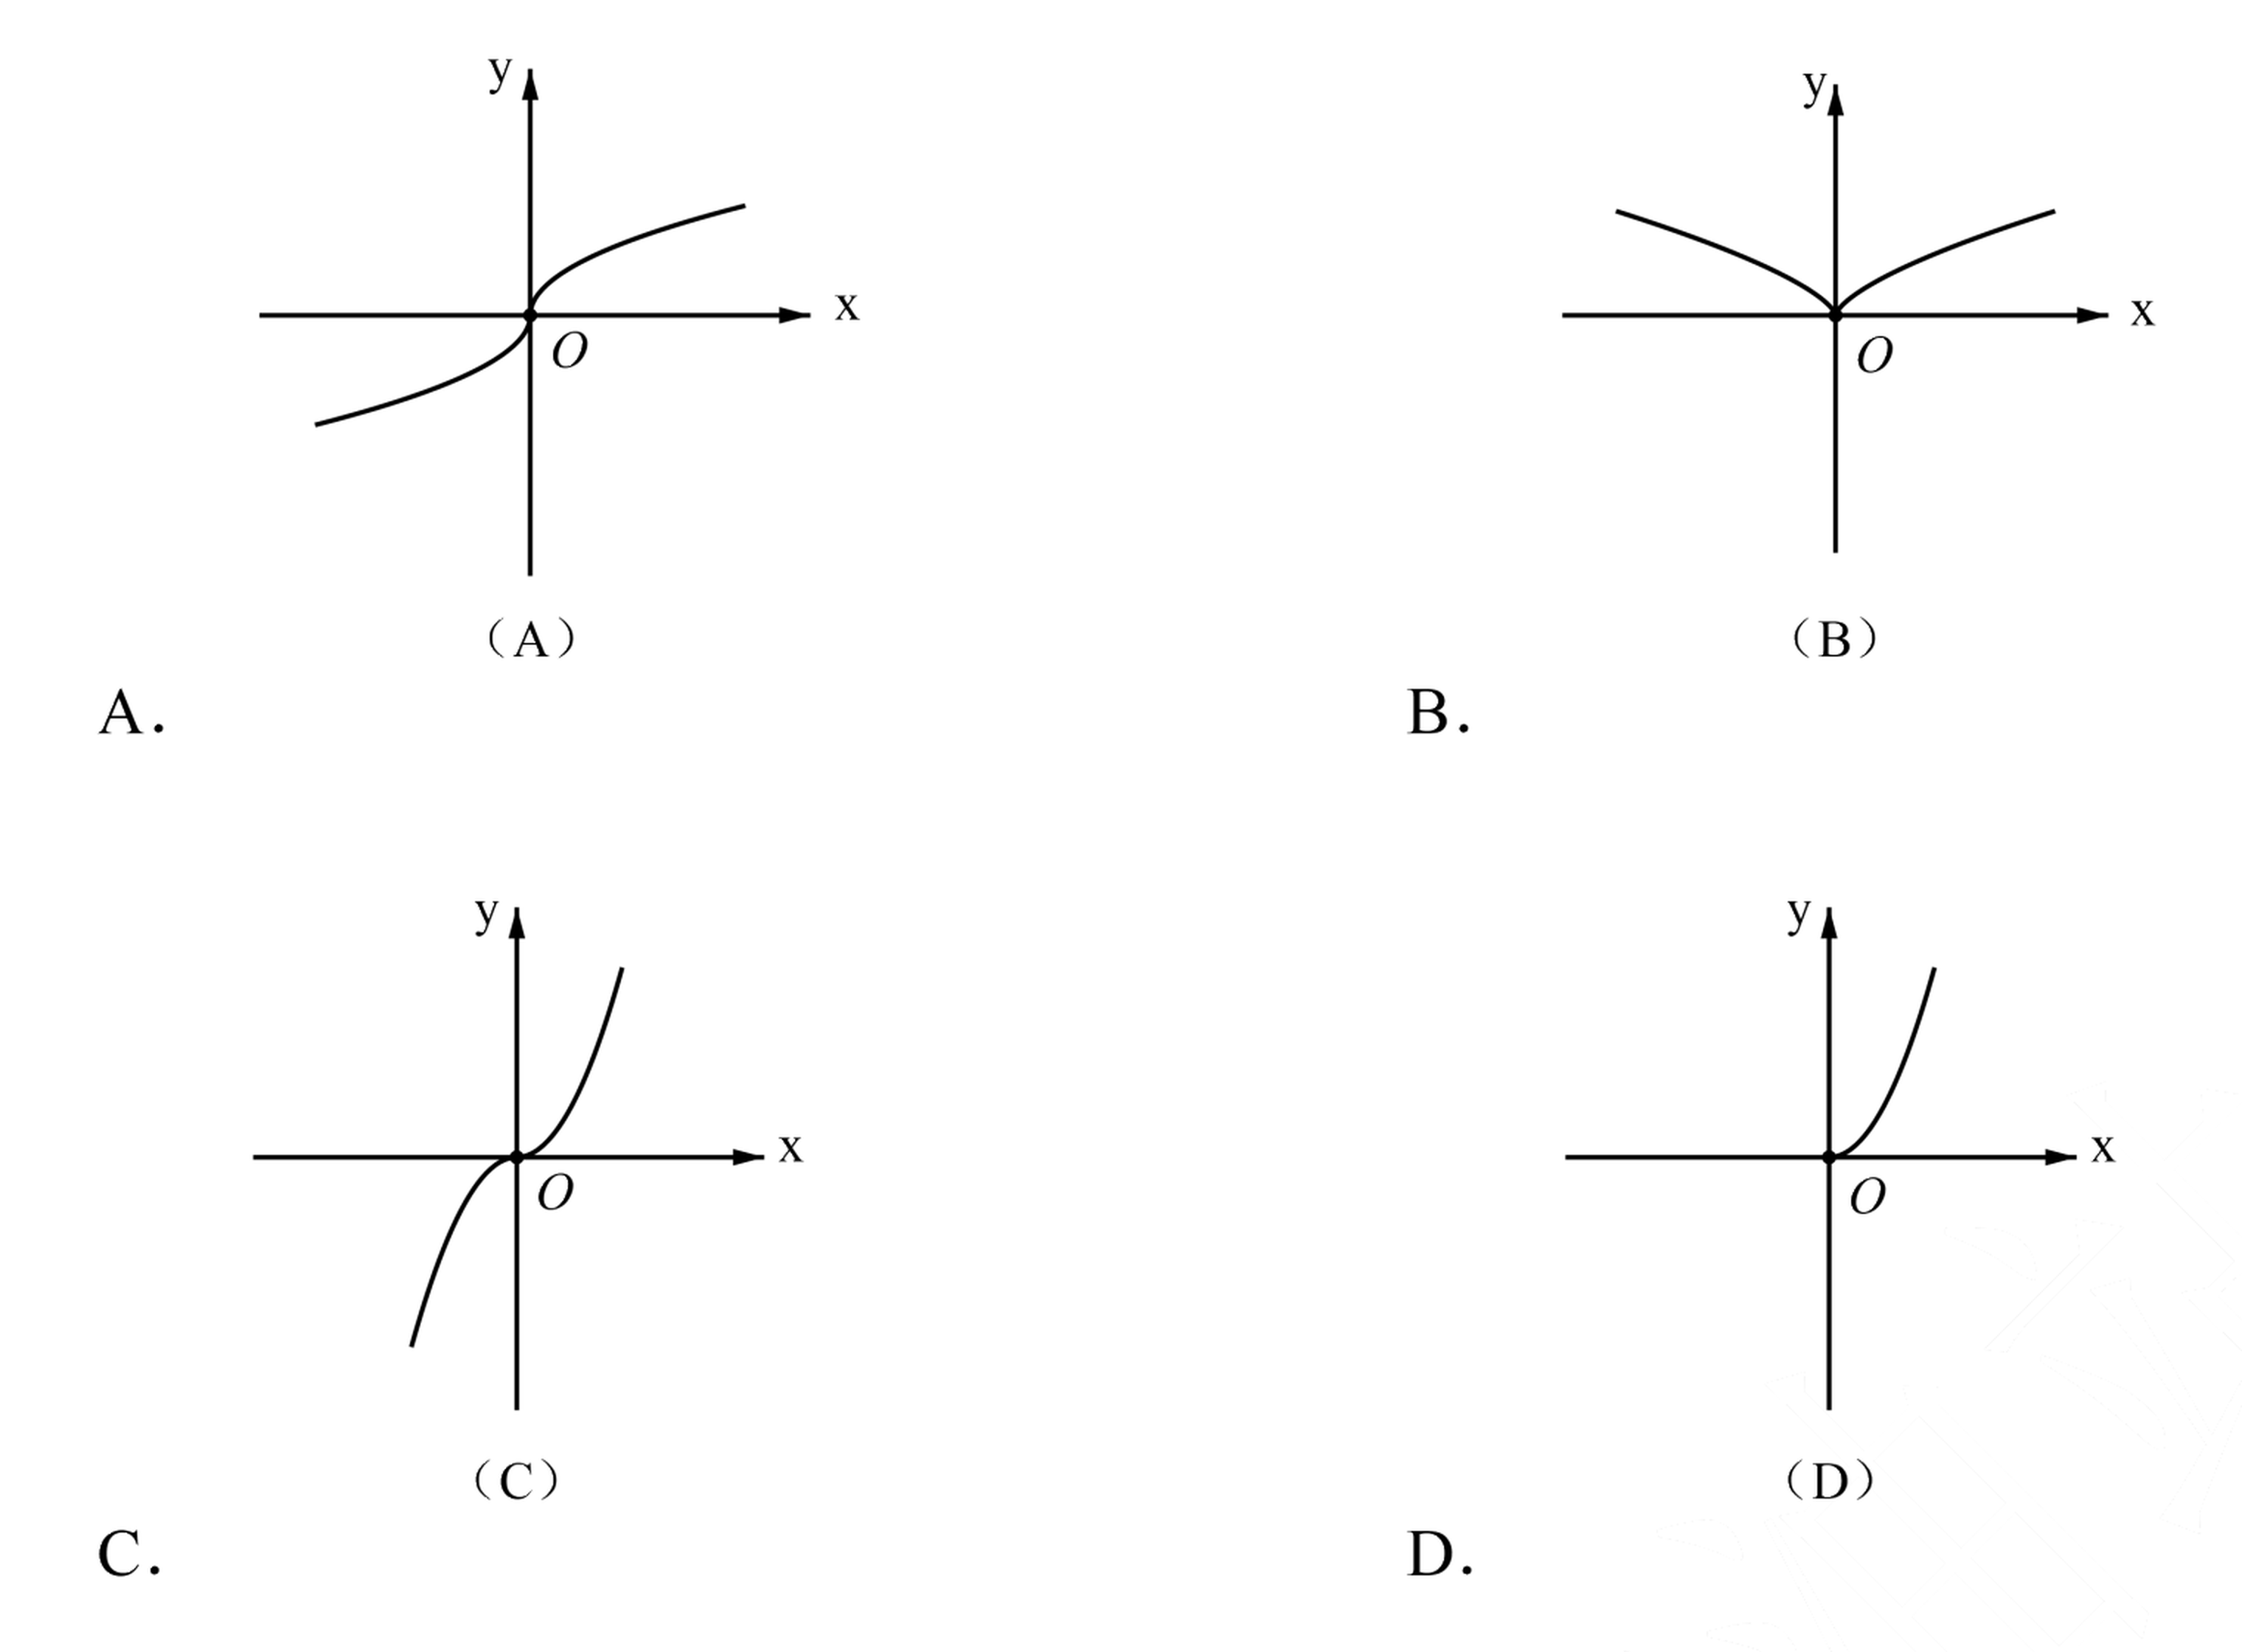
\includegraphics[width=0.80\textwidth]{figures/gao140_q14.png}
\end{center}

\ifanswer
\solbegin
\step{$f(x)=x^{\frac23}=\sqrt[3]{x^2}$ 是偶函数，且恒大于等于 $0$，故选 $B$.}
\solend
\fi

\item 设 $p$：关于 $x$ 的不等式 $x^2+ax+1>0$ 对 $x\in\R$ 恒成立，$q$：对数函数 $y=\log_{4-3a}x$ 在 $(0,+\infty)$ 上单调递减，那么 $p$ 是 $q$ 的\mbox{（\quad）}

\keepwithprev
A. 充分不必要条件\qquad B. 充要条件

C. 必要不充分条件\qquad D. 既不充分也不必要条件

\ifanswer
\solbegin
\step{$p\Leftrightarrow a^2-4<0\Leftrightarrow -2<a<2$. $q\Leftrightarrow 0<4-3a<1\Leftrightarrow 1<a<\dfrac43$.}
\step{由 $\left(1,\dfrac43\right)\subset(-2,2)$ 得 $q\Rightarrow p$；而 $a=0$ 时 $p$ 真、$q$ 假，}% 子集符号原卷印单线 $\subset$，照录
\step{故 $p$ 是 $q$ 的必要不充分条件，故选 $C$.}
\solend
\fi

\item “非空集合 $M$ 的元素都是集合 $P$ 的元素” 是假命题，现有下列命题：

(1) $M$ 的元素都不是 $P$ 的元素；(2) $M$ 中有不属于 $P$ 元素；% 原卷"不属于 P 元素"脱"的"字，照录

(3) $M$ 中有 $P$ 的元素；(4) $M$ 的元素不都是 $P$ 的元素，

其中真命题的个数是\mbox{（\quad）}

\keepwithprev
A. 1\qquad B. 2\qquad C. 3\qquad D. 4

\ifanswer
\solbegin
\step{由于 “非空集合 $M$ 的元素都是集合 $P$ 的元素” 是假命题，}
\step{得 “非空集合 $M$ 的元素至少有一个元素不属于集合 $P$” 是真命题.}
\step{则 (1) 不正确；(2) 正确；(3) $M$ 中不一定有 $P$ 的元素，例如 $M=\{a\}$，}
\step{则 $a\notin P$；(4) 正确.}
\step{综上，真命题只有 (2)(4). 故选 $B$.}
\solend
\fi

\end{enumerate}

\bigsec{三、解答题}

\begin{enumerate}
\setcounter{enumi}{16}

\item 设全集为 $\R$，集合 $A=\left\{x\mid\dfrac{2x}{x-1}\leqslant1\right\}$.

(1) 用区间表示集合 $A$；

(2) 若集合 $B=\{x\mid\lvert x+2\rvert+\lvert x-1\rvert=3\}$，求 $A\cup B$.

\ifanswer
\solbegin
\step{(1) 由 $\dfrac{2x}{x-1}\leqslant1\Leftrightarrow\dfrac{x+1}{x-1}\leqslant0$，故 $A=[-1,1)$，则 $\overline{A}=(-\infty,-1)\cup[1,+\infty)$；}
\step{(2) 由 $B=\{x\mid\lvert x+2\rvert+\lvert x-1\rvert=3\}=[-2,1]$，}
\step{结合上一问有 $A=[-1,1)$，所以 $A\cup B=B=[-2,1]$.}
\solend
\fi

\item (1) 已知指数函数 $y=a^x(a>0$ 且 $a\neq1)$ 在区间 $[-1,1]$ 上的最大值与最小值之和等于 $\dfrac52$，求实数 $a$ 的值.

(2) 已知幂函数 $y=x^{m^2+7m+10}(m\in\Z)$ 的图像关于 $y$ 轴对称，且在 $(0,+\infty)$ 上严格减. 若 $(a-1)^{m^2+7m+10}\geqslant(1+2a)^{m^2+7m+10}$. 求实数 $a$ 的取值范围.

\ifanswer
\solbegin
\step{(1) 指数函数 $y=a^x$ 在区间 $[-1,1]$ 上单调，所以 $a^1+a^{-1}=\dfrac52$，}
\step{所以 $a=2$ 或 $a=\dfrac12$；}
\step{(2) 由题意得 $m^2+7m+10<0$，所以 $-5<m<-2$，又因为 $m\in\Z$，}
\step{所以 $m=-4$ 或 $m=-3$，}
\step{当 $m=-4$ 时，$y=x^{m^2+7m+10}=x^{-2}$，为偶函数，}
\step{当 $m=-3$ 时，$y=x^{m^2+7m+10}=x^{-2}$，为偶函数，}
\step{所以 $m^2+7m+10=-2$，所以 $(a-1)^{-2}\geqslant(1+2a)^{-2}$，}
\step{所以 $\lvert a-1\rvert\leqslant\lvert 1+2a\rvert$，所以 $a\leqslant-2$ 或 $a\geqslant0$，所以 $a\in(-\infty,-2]\cup[0,+\infty)$.}
\solend
\fi

\item 设函数 $f(x)=ax^2+(1-a)x+a-2$ （$a\in\R$）.

(1) 若关于 $x$ 的不等式 $f(x)\leqslant0$ 的解集为 $\left[0,\dfrac12\right]$，求实数 $a$ 的值；

(2) 若 $a\geqslant0$，解关于 $x$ 的不等式：$f(x)<a-1$.

\ifanswer
\solbegin
\step{(1) 由解集得 $a>0$，且 $0$ 是方程 $f(x)=0$ 的根，故 $f(0)=a-2=0$，}
\step{得 $a=2$.}
\step{此时 $f(x)=2x^2-x=x(2x-1)$，$f(x)\leqslant0$ 的解集确为 $\left[0,\dfrac12\right]$.}
\step{(2) $f(x)<a-1\Leftrightarrow ax^2+(1-a)x-1<0\Leftrightarrow(x-1)(ax+1)<0$，}
\step{当 $a=0$ 时，$x-1<0$，解集为 $(-\infty,1)$.}
\step{当 $a>0$ 时，$-\dfrac1a<1$，解集为 $\left(-\dfrac1a,1\right)$.}
\solend
\fi

\item 为了保护环境，某单位采用新工艺，把二氧化碳转化为一种可利用的化工产品，已知该单位每月处理量最多不超过 $300$ 吨. 当月处理量为 $x$ 吨时，月处理成本为 $x^2-200x+40000(0<x\leqslant300)$ 元，且每处理一吨二氧化碳得到可利用的化工产品价值为 $300$ 元.

(1) 若要保证该单位每月不亏损，则每月处理量应控制在什么范围？

(2) 该单位每月处理量为多少吨时，才能使每吨的平均处理成本最低，最低为多少元？

\ifanswer
\solbegin
\step{(1) 由题意得 $S=300x-(x^2-200x+40000)$}
\step{$=-x^2+500x-40000(0<x\leqslant300)$，}
\step{令 $S\geqslant0$，即 $-x^2+500x-40000\geqslant0$，解得 $100\leqslant x\leqslant400$，}
\step{又 $0<x\leqslant300$，所以 $100\leqslant x\leqslant300$，}
\step{故要保证该单位每月不亏损，则每月处理量应控制在 $[100,300]$ 范围内；}
\step{(2) 每吨的平均出来成本为 $\dfrac yx=x+\dfrac{40000}x-200\geqslant2\sqrt{x\cdot\dfrac{40000}x}-200=200$，}% 原卷"平均出来成本"与题干"平均处理成本"措辞不一，照录
\step{当且仅当 $x=\dfrac{40000}x$，即 $x=200$ 时取等号，}
\step{所以该单位每月处理量为 $200$ 吨时，}
\step{才能使每吨的平均处理成本最低且最低为 $200$ 元.}
\solend
\fi

\item 已知函数 $y=f(x),x\in D$，若对于定义域 $D$ 内任意实数 $x,y$，不等式 $f(x)+f(y)\geqslant f(xy)$ 都成立，则称函数 $y=f(x)$ 是 $QB$ 函数，

(1) 判断函数 $f(x)=x+1$ 是否是 $QB$ 函数，并说明理由；

(2) 若函数 $g(x)=\ln(ax),x>0$ 是 $QB$ 函数，求实数 $a$ 的取值范围；

(3) 已知函数 $h(x)=a^x(a\in\R\text{ 且 }a>0)$，证明：“函数 $y=h(x)$ 是 $QB$ 函数” 的充要条件是 “ $a\in\{1\}$ ”.

\ifanswer
\solbegin
\step{(1) 不是，理由如下：因为 $f(x)=x+1$，}
\step{所以 $f(x)+f(y)\geqslant f(xy)\Leftrightarrow x+y\geqslant xy-1\Leftrightarrow(x-1)(y-1)\leqslant2$，}
\step{显然不恒成立，故不是 $QB$ 函数；}
\step{(2) 因为函数 $g(x)=\ln(ax),x>0$，则 $a>0$，}
\step{若函数 $g(x)$ 是 $QB$ 函数，则 $g(x)+g(y)\geqslant g(xy)$，}
\step{即 $\ln(ax)+\ln(ay)\geqslant\ln(axy)$，则 $\ln(a^2xy)\geqslant\ln(axy)$，得 $a^2xy\geqslant axy$，}
\step{且 $x>0,y>0$，得 $a^2\geqslant a$，解得 $a\geqslant1$ 或 $a\leqslant0$（舍去），}
\step{所以实数 $a$ 的取值范围为 $[1,+\infty)$.}
\step{(3) 若函数 $h(x)=a^x$ 是 $QB$ 函数，}
\step{当 $a>1$ 时，令 $x=y=\log_a\dfrac12$，则 $h(x)+h(y)=a^x+a^y=\dfrac12+\dfrac12=1$，}
\step{且 $h(xy)=a^{xy}=(a^x)^y=\left(\dfrac12\right)^{\log_a\frac12}=2^{\log_a2}$，}
\step{因为 $\log_a2>0$，所以 $h(xy)=2^{\log_a2}>1$，不满足 $h(x)+h(y)\geqslant h(xy)$，}
\step{不合题意；}
\step{当 $a=1$ 时，$h(x)+h(y)=a^x+a^y=1+1=2$，且 $h(xy)=a^{xy}=1$，}
\step{满足 $h(x)+h(y)\geqslant h(xy)$，符合题意；}
\step{当 $0<a<1$ 时，令 $x=\log_a2,y=2$，则 $h(x)+h(y)=a^x+a^y=2+a^2$，}
\step{且 $h(xy)=a^{xy}=(a^x)^y=2^2=4$，}
\step{因为 $0<a<1$，所以 $0<a^2<1$，得 $2<2+a^2<3$，}
\step{不满足 $h(x)+h(y)\geqslant h(xy)$，不合题意；}
\step{综上所述，$a\in\{1\}$，即充分性成立；}% 原卷"充分性/必要性"两标签与所证方向互换，照录
\step{若 $a\in\{1\}$，则 $h(x)+h(y)=a^x+a^y=1+1=2$，且 $h(xy)=a^{xy}=1$，}
\step{得 $h(x)+h(y)\geqslant h(xy)$，所以函数 $h(x)=a^x$ 是 $QB$ 函数，即必要性成立；}% 原卷"充分性/必要性"两标签与所证方向互换，照录
\step{综上所述，“函数 $y=h(x)$ 是 $QB$ 函数” 的充要条件是 “ $a\in\{1\}$ ”.}
\solend
\fi

\end{enumerate}

\end{document}
"
% 紧凑版：xelatex "\def\iscompact{1}% 高一140_甘泉外国语_期中.tex
%   —— 高一上数学"2026-2027 年甘泉外国语高一上期中"（试卷版/答案版）
% 试卷版：xelatex 高一140_甘泉外国语_期中.tex
% 答案版：xelatex "\def\isanswer{1}\input{高一140_甘泉外国语_期中.tex}"
% 紧凑版：xelatex "\def\iscompact{1}\input{高一140_甘泉外国语_期中.tex}"
%
% ① 原始材料：微信公众号"魔都数学加油站"文章，连载"27学年高一140"，原文标题
% "27学年高一140——2026-2027年上海市甘泉外国语高一上期中"；
% 原文链接：https://mp.weixin.qq.com/s/eflgf2Ktk1LyT9x-k-ltLw。
% 正文为 9 张 PNG 页（01、02、03、05、06、07、08 为 4762x6735；04、09 为 2560x3620，
% 同一篇各页分辨率不同，逐页按各自分辨率裁图核对），题目下印有【答案】或【解析】，为讲评版。
% 题目、解析均据原图转录；卷面粉红色水印"魔都数学加油站"及公众号页脚未录入。
% 全卷 1 幅插图：第 14 题四幅坐标函数图象选项（04 页），取原卷截图去粉色水印、去色、
% LANCZOS 放大 2 倍，四幅选项按原卷 2x2 排布（含（A）（B）（C）（D）图注与 A./B./C./D.
% 选项字母）合并裁为一张；图前按惯例加 \needvspace 守卫。
%
% 卷首标题：原卷印作"2026-2027 年甘泉外国语高一上期中"（公众号标题中的"上海市"
% 卷面标题行没有，本稿照卷面），年份区间按全稿惯例排 en dash；原卷未印副标题，
% 本卷为期中卷、跨集合与常用逻辑用语／不等式／函数三章，按题目内容标为
% "集合与常用逻辑用语、不等式、函数"（与 125／126／128／129／131／132／133 同期中卷口径相同）：
% 集合与逻辑见 Q5、Q13、Q15、Q16、Q17，不等式见 Q3、Q10、Q11、Q19、Q20，
% 函数（指数／对数／幂函数及其图象、同构与 QB 函数）见 Q4、Q6、Q7、Q8、Q12、Q14、Q18、Q21。
%
% 题号体例：本卷共 19 题——一、填空题 3—12（10 题）、二、选择题 13—16（4 题）、
% 三、解答题 17—21（5 题）。三节分别 \setcounter{enumi}{2}／{12}／{16}。
% 原卷从第 3 题起、无第 1、2 题，本稿保留原题号。
%
% ② 与原卷的排版差异：
%   ① 原文从第 3 题起，本稿保留原题号；
%   ② 原卷每题下直接印【答案】或【解析】，本稿按全稿惯例置于答案版；第 5 题只印
%      【答案】、无【解析】，提 \ans{}；第 13、14、15、16 题答案均在【解析】末句
%      "故选 …"，题干括号内留空、不另提 \ans{}；其余各题印【解析】、无独立答案段；
%      全卷无"答案印在题干括号内且无解析"的一型；
%   ③ 原卷未印副标题，本稿按"知识模块"口径补出；
%   ④ 原卷填空横线按全稿惯例排为 \blankline[4.4em]；选择题括号排 \mbox{（\quad）}、
%      每个选项段前按惯例加 \keepwithprev（四幅图选项那一枚放在 \begin{center} 之前）；
%      解答题不留作答区、不加 \anspace（原卷为讲评版，与 129／131／132／133／136 同）；
%   ⑤ 原卷数集混排：斜体 $R$（Q9、Q12、Q15 等）与黑体／黑板粗体 $R$（Q15、Q17、
%      Q19、Q21）、粗体 $Z$（Q18），按全稿惯例统一改 \R／\Z；空集记号 \varnothing；
%      绝对值排 \lvert…\rvert，集合描述竖线排 \mid；不等号按全稿惯例排 \leqslant／\geqslant；
%      补集照原卷上划线排 \overline{A}；
%   ⑥ 子题标号 (1)(2)(3)(4) 原卷印半角括号，照录（与 131／132／133／134／136 同口径）；
%      括注原卷全角／半角混用，逐处照录：Q8"（结果用 a,b 表示）"、Q19"（a∈R）"、
%      Q21 (2)"（舍去）"印全角，Q18"$a^x(a>0$ 且 $a\neq1)$"、Q20"$40000(0<x\leqslant300)$"、
%      Q21 (3)"($a\in\R$ 且 $a>0$)"及 (0,+∞)、2(a>0) 等数学式内括注印半角；
%   ⑦ 数学式内半角逗号照录（如 Q8"$\lg2=a,10^b=3$"、Q11"$-2,3,4,\cdots,2027$"、
%      Q12"$x_1,x_2$"、Q19"$f(x)=ax^2+(1-a)x+a-2$"、Q21"$x>0,y>0$"）；
%      原卷行末西文句点照录（Q20 题干"300 吨. 当月处理量为 x 吨时"），行中全角逗号照录；
%   ⑧ 一幅插图：第 14 题四幅坐标函数图象选项合并裁为一张 \includegraphics
%      （题前 \needvspace{9cm}）。Q14 是"二、选择题"节内带大图块的第二题
%      （Q13 为节首题但无图），另在 \bigsec{二、选择题} 之前加 \needvspace{11cm}
%      连节标题一起量——守卫必须放在 \bigsec 之前，放标题之后会让"二、选择题"
%      孤立在页末（B 类，照 高一26／40／59／136 成例）；三版切页审计均"合计异常：无"；
%   ⑨ 跨页续印按题合并：Q9 题干在 01 页、解析续至 02 页；Q11 题干与解析前 3 行在 02 页、
%      后 2 行在 03 页；Q14 题干在 03 页末、四幅图与【解析】在 04 页；Q16 题干四条命题
%      在 04 页、选项与【解析】在 05 页；Q18 解析 (1) 首行在 05 页、其余 7 行在 06 页；
%      Q20 题干在 06 页末、"300 元."与两小问及【解析】在 07 页；Q21 解析跨 07—09 页
%      （末 3 行在 09 页）；本稿按题连排，不丢行；
%   ⑩ 题干中的中文弯引号按原卷照录，注释内一律 ASCII 引号；原卷"图像／图象"
%      两种写法混用，逐处照录（Q7、Q18 作"图像"，Q14 作"图象"）；
%   ⑪ 原卷无红色加粗标签（【解析】【答案】均黑色印刷），故本卷未用 \stepm。
%
% 判别式字形：全卷仅第 9 题【解析】"经验证得"cases 块出现两处判别式
%   "$\Delta=p^2-4q>0$"与"$\Delta'=q^2-4p>0$"，原卷两处均印等腰、偏高的
%   三角 $\Delta$（带撇的为 $\Delta'$），逐处放大核对并照录 \Delta、\Delta'；
%   全卷未出现扁等边三角 \triangle。
%
% 子集符号：第 15 题【解析】"由 (1,4/3)⊂(-2,2) 得 q⇒p"一处原卷印单线 $\subset$
%   （不带下划线），逐处放大核对、照录 \subset；全卷未出现带下划线的 \subseteq。
%
% 原卷存疑照录（均照录未改，正文对应处另有 % 注）：
%   第 16 题 (2) 命题"$M$ 中有不属于 $P$ 元素"中"不属于 $P$ 元素"脱"的"字，照录；
%   第 20 题题干 (2) 作"每吨的平均处理成本"、而【解析】(2) 作"每吨的平均出来成本"，
%      "出来"疑为"处理"之误，两处措辞照录不统一；
%   第 21 题 (3)【解析】"综上所述，$a\in\{1\}$，即充分性成立"与"即必要性成立"
%      两处标签与所证方向互换（按充要条件的通常口径），照录。
%
% 行数复核：一条 \step = 原卷解析的一个印刷行，cases 块作一个印刷行计。逐题数 \step
%   条数，合计 92 条（Q3：2；Q4：1；Q5：0；Q6：2；Q7：1；Q8：1；Q9：7；Q10：5；
%   Q11：5；Q12：4；Q13：6；Q14：1；Q15：3；Q16：5；Q17：3；Q18：8；Q19：6；
%   Q20：9；Q21：23），与原卷印刷行逐题相等。第 5 题只印【答案】、提 \ans{}，
%   不计入 \step 账；第 13、14、15、16 题答案在解析末句"故选 …"，括号内留空、
%   不另提 \ans{}；答案版【答案】/【解析】标记数 = 19（1 个 \ans + 18 个 \solbegin）
%   = 全卷题数。
%
\documentclass[a4paper,11pt]{article}
\usepackage{common}

\begin{document}

\examtitlest[3]{2026--2027 年甘泉外国语高一上期中}{集合与常用逻辑用语、不等式、函数}

\bigsec{一、填空题}

\begin{enumerate}
\setcounter{enumi}{2}

\item 不等式 $x^2-2x-3<0$ 的解集为\blankline[4.4em].

\ifanswer
\solbegin
\step{方程 $x^2-2x-3=0$ 的实数根是 $x_1=-1$，$x_2=3$；}
\step{所以不等式 $x^2-2x-3<0$ 的解集为 $\{x\mid -1<x<3\}$.}
\solend
\fi

\item 根式 $\sqrt{x\sqrt{x}}(x>0)$ 的指数幂形式为\blankline[4.4em].

\ifanswer
\solbegin
\step{$\sqrt{x\sqrt{x}}=\sqrt{x\cdot x^{\frac12}}=\sqrt{x^{\frac32}}=x^{\frac34}$.}
\solend
\fi

\item 陈述句 “ $x>1$ 或 $y>1$ ” 的否定形式是\blankline[4.4em].

\ifanswer
\ans{$x\leqslant1$ 且 $y\leqslant1$}
\fi

\item 若 $x<0$ 时，指数函数 $y=(a-1)^x$ 的值总大于 $1$，则实数 $a$ 的取值范围是\blankline[4.4em].

\ifanswer
\solbegin
\step{由题意得 $(a-1)^x>1$ 在 $(-\infty,0)$ 上恒成立，则 $0<a-1<1$，解得 $1<a<2$.}
\step{故实数 $a$ 的取值范围是 $(1,2)$.}
\solend
\fi

\item 若 $f(x)=\log_a(x-1)$，对任意 $a>0$ 且 $a\neq1$，函数 $y=f(x)$ 的图像必过定点\blankline[4.4em].

\ifanswer
\solbegin
\step{令 $x-1=1$，即 $x=2$，此时 $f(2)=0$，即函数图像过定点 $(2,0)$.}
\solend
\fi

\item 已知 $\lg 2=a,10^b=3$，则 $\log_6 2=$\blankline[4.4em]（结果用 $a,b$ 表示）.

\ifanswer
\solbegin
\step{由 $10^b=3$，得 $b=\lg 3$，则 $\log_6 2=\dfrac{\lg 2}{\lg 6}=\dfrac{\lg 2}{\lg 2+\lg 3}=\dfrac{a}{a+b}$.}
\solend
\fi

\item 已知 $p$、$q\in\R$，$x_1$、$x_2$ 是关于 $x$ 的方程 $x^2+px+q=0$ 的两实根，$x_1+1$、$x_2+1$ 是关于 $x$ 的方程 $x^2+qx+p=0$ 的两实根，则 $pq=$\blankline[4.4em].

\ifanswer
\solbegin
\step{因为 $x_1$、$x_2$ 是关于 $x$ 的方程 $x^2+px+q=0$ 的两实根，}
\step{由韦达定理得 $x_1+x_2=-p$，$x_1\cdot x_2=q$，}
\step{因为 $x_1+1$、$x_2+1$ 是关于 $x$ 的方程 $x^2+qx+p=0$ 的两实根，}
\step{由韦达定理得 $x_1+1+x_2+1=-q$，$(x_1+1)(x_2+1)=p$，}
\step{即 $x_1+x_2=-q-2$，$x_1+x_2+x_1x_2=p-1$，又 $x_1+x_2=-p$，$x_1\cdot x_2=q$，}
\step{所以 $\begin{cases}-p=-q-2\\-p+q=p-1\end{cases}$，解得 $\begin{cases}p=-1\\q=-3\end{cases}$，经验证得 $\begin{cases}\Delta=p^2-4q>0\\\Delta'=q^2-4p>0\end{cases}$，}% 判别式原卷印高三角 $\Delta$、$\Delta'$，照录
\step{则 $pq=3$.}
\solend
\fi

\item 对于 $x\in\R$，不等式 $\lvert 3-x\rvert+\lvert 1+x\rvert\geqslant a^2-3a$ 恒成立，则实数 $a$ 的取值范围是\blankline[4.4em].

\ifanswer
\solbegin
\step{对于 $x\in\R$，不等式 $\lvert 3-x\rvert+\lvert 1+x\rvert\geqslant a^2-3a$ 恒成立，}
\step{即 $\lvert 3-x\rvert+\lvert 1+x\rvert$ 的最小值大于或等于 $a^2-3a$，}
\step{$\lvert 3-x\rvert+\lvert 1+x\rvert$ 表示数轴上的 $x$ 对应点到 $3$ 和 $-1$ 对应点的距离之和，}
\step{它的最小值为 $4$，故 $4\geqslant a^2-3a$，即 $a^2-3a-4\leqslant0$，解得 $-1\leqslant a\leqslant4$，}
\step{故实数 $a$ 的取值范围是 $[-1,4]$.}
\solend
\fi

\item 已知同时满足不等式 $x^2-x-2>0$ 和 $2x^2+(5+2a)x+5a<0$ 的 $x$ 的整数值只有 $2026$ 个，则实数 $a$ 的取值范围是\blankline[4.4em].

\ifanswer
\solbegin
\step{整数 $x$ 须满足 $x\leqslant-2$ 或 $x\geqslant3$，且 $(2x+5)(x+a)<0$.}
\step{当 $a<\dfrac52$ 时，需使整数解恰为 $-2,3,4,\cdots,2027$，即 $2027<-a\leqslant2028$.}
\step{当 $a>\dfrac52$ 时，需使整数解恰为 $-2028,-2027,\cdots,-3$，即 $2028<a\leqslant2029$；}
\step{$a=\dfrac52$ 时无解.}
\step{故 $a\in[-2028,-2027)\cup(2028,2029]$.}
\solend
\fi

\item 同构式通俗讲是结构相同的表达式，如：$f(x)=x+e^x$，$f(\ln x)=\ln x+e^{\ln x}=\ln x+x$，称 $x+e^x$ 与 $\ln x+x$ 为同构式. 已知实数 $x_1,x_2$ 满足 $e^{x_1}+x_1=8,\ln\sqrt[5]{5x_2+3}+x_2=1$，则 $x_1+5x_2=$\blankline[4.4em].

\ifanswer
\solbegin
\step{函数 $f(x)=x+e^x$ 在 $\R$ 上严格增，且 $f(x_1)=x_1+e^{x_1}=8$，}
\step{由 $\ln\sqrt[5]{5x_2+3}+x_2=1$，得 $\ln(5x_2+3)+5x_2=5$，则 $\ln(5x_2+3)+5x_2+3=8$，}
\step{即 $f(\ln(5x_2+3))=8$，因此 $f(\ln(5x_2+3))=8=f(x_1)$，则 $x_1=\ln(5x_2+3)$，}
\step{所以 $x_1+5x_2=\ln(5x_2+3)+5x_2=5$.}
\solend
\fi

\end{enumerate}

% 第 14 题四幅图是"二、选择题"节内的大图块；守卫须放在 \bigsec 之前连节标题一起量，
% 否则"二、选择题"会孤立在页末（B 类，照 高一26／40／59／136 成例）
\needvspace{11cm}
\bigsec{二、选择题}

\begin{enumerate}
\setcounter{enumi}{12}

\item 设 $a$、$b$ 为实数，则 “ $a>b>0$ ” 的一个充分非必要条件是\mbox{（\quad）}

\keepwithprev
A. $\sqrt{a-1}>\sqrt{b-1}$\qquad B. $a^2>b^2$

C. $\dfrac1b>\dfrac1a$\qquad D. $a-b>b-a$

\ifanswer
\solbegin
\step{由 $\sqrt{a-1}>\sqrt{b-1}$ 得 $a>b\geqslant1$，故 $a>b>0$，反之不成立，满足题意；}
\step{由 $a^2>b^2$，则 $\lvert a\rvert>\lvert b\rvert$，推不出 $a>b>0$，反向可推出，不满足；}
\step{由 $\dfrac1b>\dfrac1a$，则 $a>b>0$ 或 $b>0>a$ 或 $0>a>b$，推不出 $a>b>0$，}
\step{反向可推出，不满足；}
\step{由 $a-b>b-a$，则 $a>b$，推不出 $a>b>0$，反向可推出，不满足；}
\step{故选 $A$.}
\solend
\fi

% 第 14 题四幅坐标函数图象选项是一整块，守卫放在 \item 之前
\needvspace{9cm}
\item 幂函数 $f(x)=x^{\frac23}$ 的图象大致为\mbox{（\quad）}

\keepwithprev
\begin{center}
% 四幅坐标函数图象选项取原卷 04 页截图去粉色水印、去色，按原卷 2x2 排布合并为一张
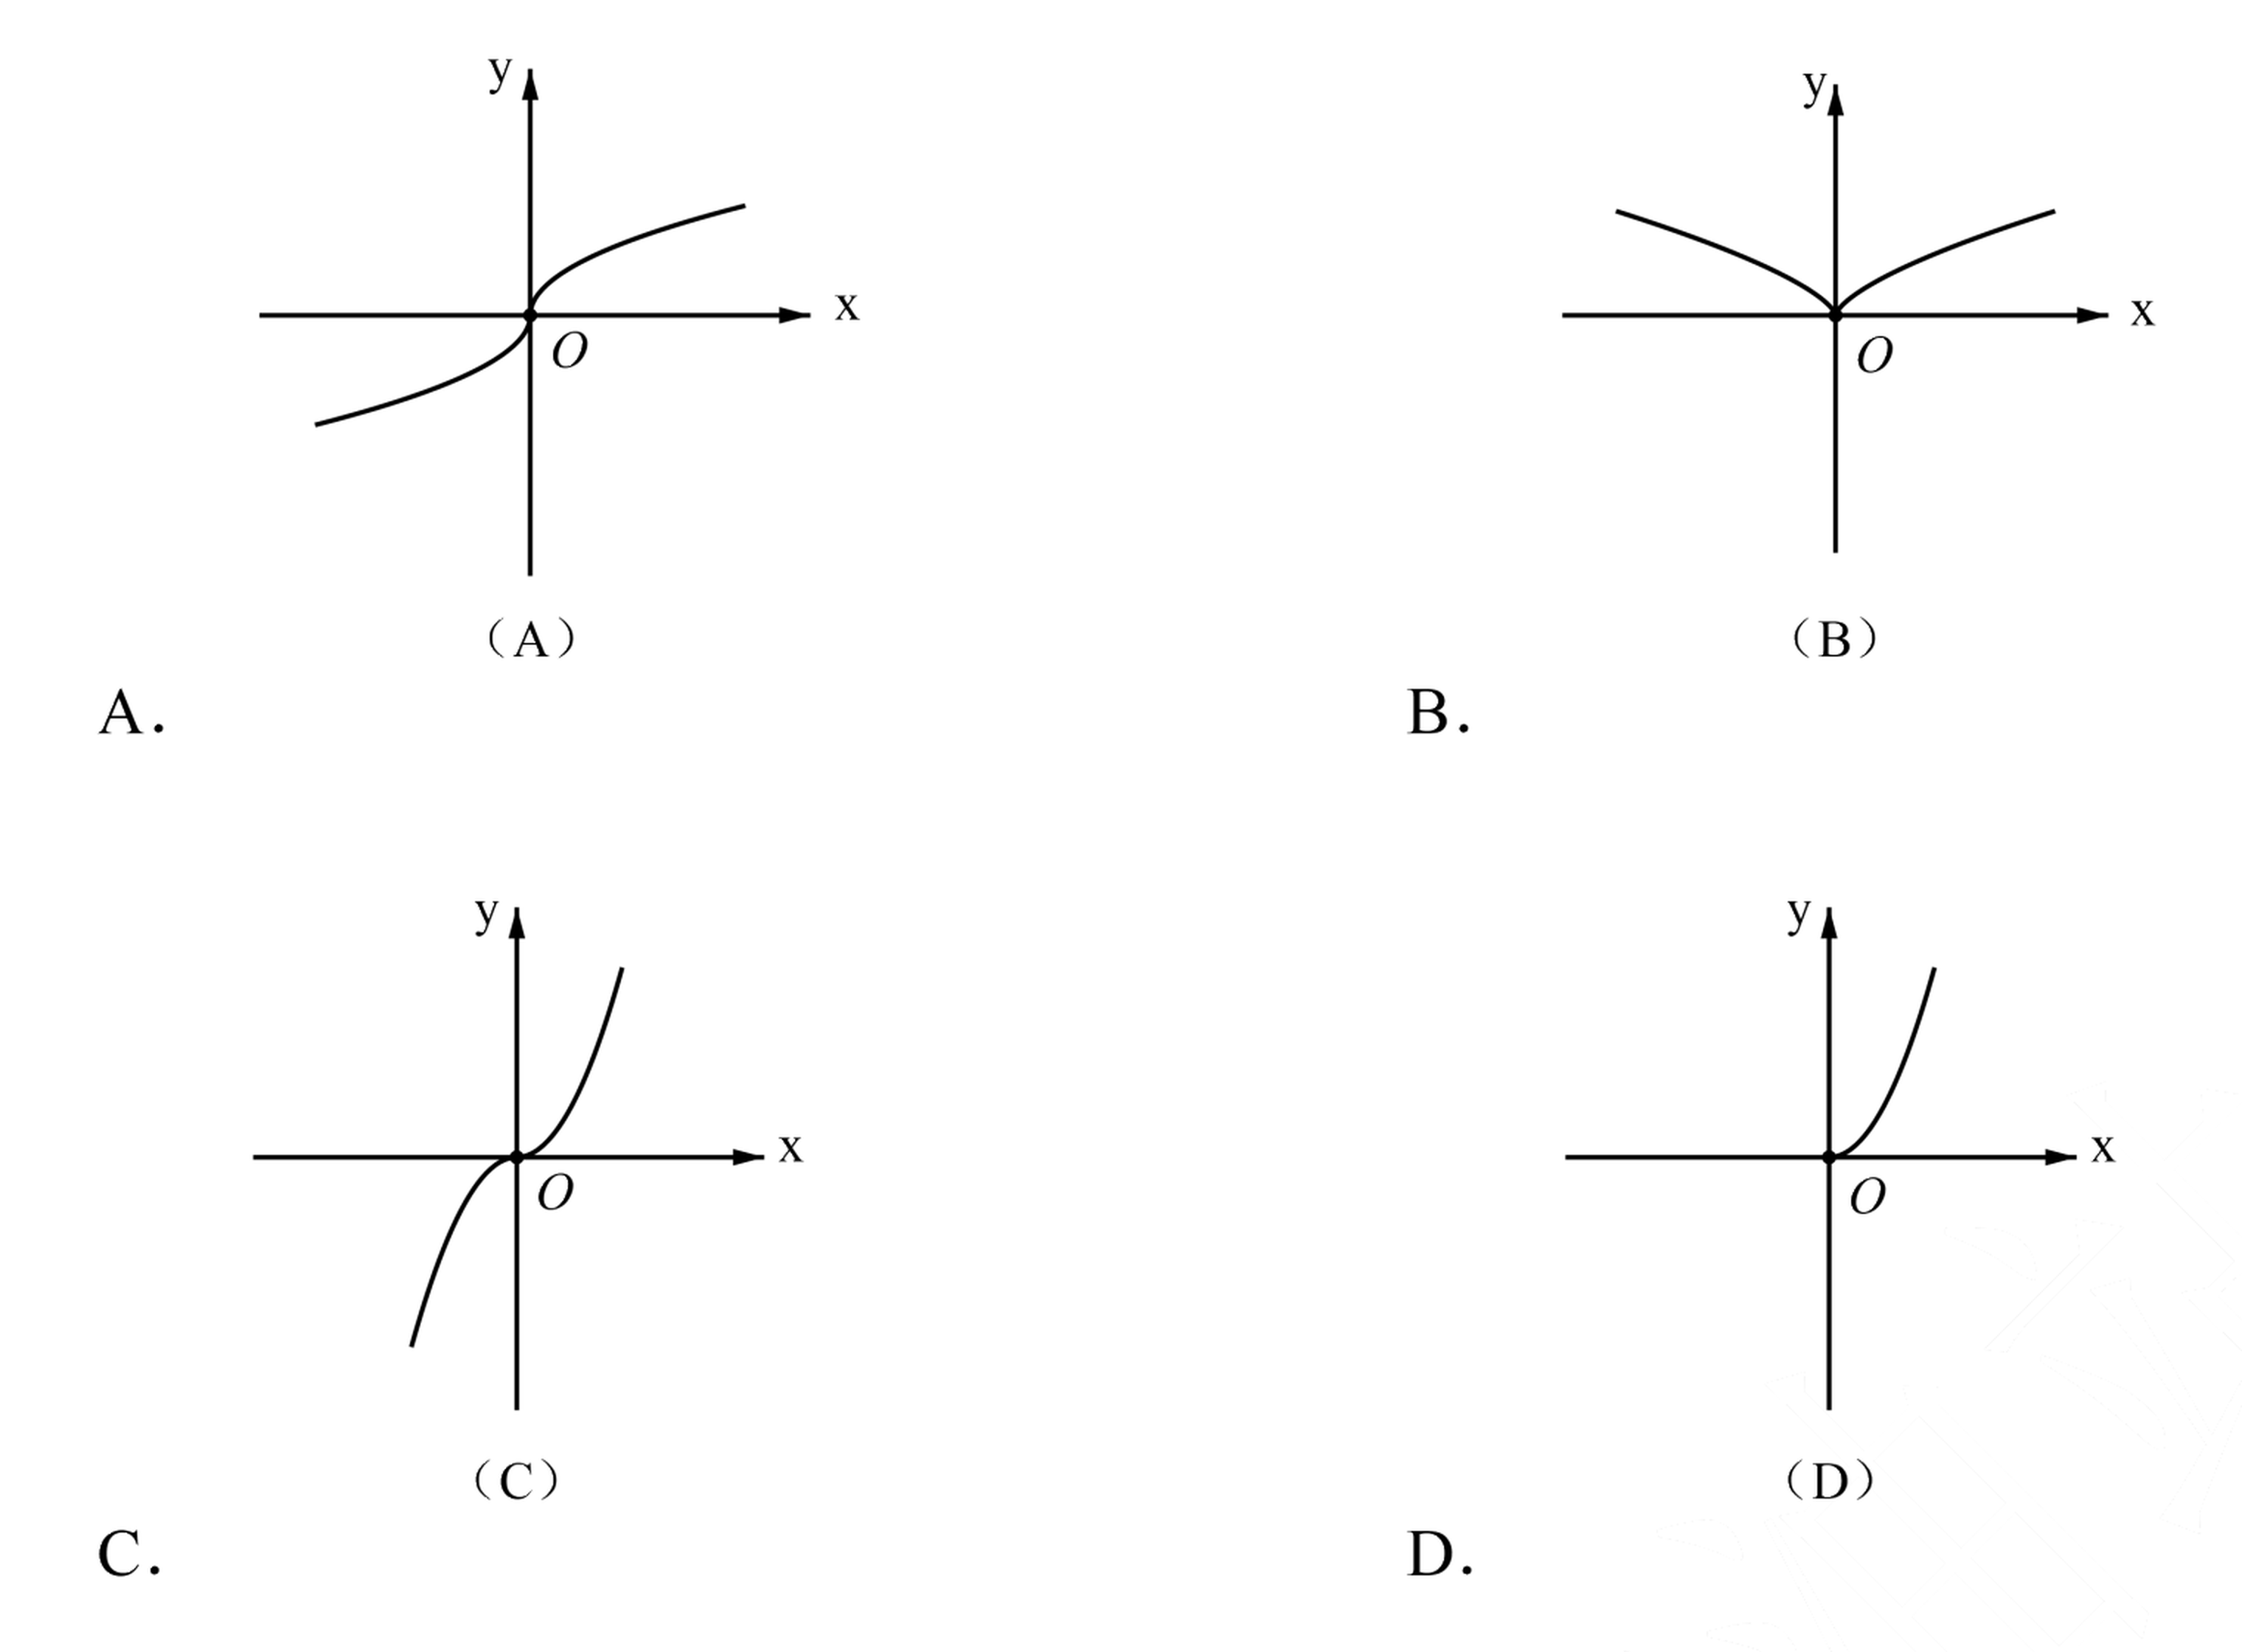
\includegraphics[width=0.80\textwidth]{figures/gao140_q14.png}
\end{center}

\ifanswer
\solbegin
\step{$f(x)=x^{\frac23}=\sqrt[3]{x^2}$ 是偶函数，且恒大于等于 $0$，故选 $B$.}
\solend
\fi

\item 设 $p$：关于 $x$ 的不等式 $x^2+ax+1>0$ 对 $x\in\R$ 恒成立，$q$：对数函数 $y=\log_{4-3a}x$ 在 $(0,+\infty)$ 上单调递减，那么 $p$ 是 $q$ 的\mbox{（\quad）}

\keepwithprev
A. 充分不必要条件\qquad B. 充要条件

C. 必要不充分条件\qquad D. 既不充分也不必要条件

\ifanswer
\solbegin
\step{$p\Leftrightarrow a^2-4<0\Leftrightarrow -2<a<2$. $q\Leftrightarrow 0<4-3a<1\Leftrightarrow 1<a<\dfrac43$.}
\step{由 $\left(1,\dfrac43\right)\subset(-2,2)$ 得 $q\Rightarrow p$；而 $a=0$ 时 $p$ 真、$q$ 假，}% 子集符号原卷印单线 $\subset$，照录
\step{故 $p$ 是 $q$ 的必要不充分条件，故选 $C$.}
\solend
\fi

\item “非空集合 $M$ 的元素都是集合 $P$ 的元素” 是假命题，现有下列命题：

(1) $M$ 的元素都不是 $P$ 的元素；(2) $M$ 中有不属于 $P$ 元素；% 原卷"不属于 P 元素"脱"的"字，照录

(3) $M$ 中有 $P$ 的元素；(4) $M$ 的元素不都是 $P$ 的元素，

其中真命题的个数是\mbox{（\quad）}

\keepwithprev
A. 1\qquad B. 2\qquad C. 3\qquad D. 4

\ifanswer
\solbegin
\step{由于 “非空集合 $M$ 的元素都是集合 $P$ 的元素” 是假命题，}
\step{得 “非空集合 $M$ 的元素至少有一个元素不属于集合 $P$” 是真命题.}
\step{则 (1) 不正确；(2) 正确；(3) $M$ 中不一定有 $P$ 的元素，例如 $M=\{a\}$，}
\step{则 $a\notin P$；(4) 正确.}
\step{综上，真命题只有 (2)(4). 故选 $B$.}
\solend
\fi

\end{enumerate}

\bigsec{三、解答题}

\begin{enumerate}
\setcounter{enumi}{16}

\item 设全集为 $\R$，集合 $A=\left\{x\mid\dfrac{2x}{x-1}\leqslant1\right\}$.

(1) 用区间表示集合 $A$；

(2) 若集合 $B=\{x\mid\lvert x+2\rvert+\lvert x-1\rvert=3\}$，求 $A\cup B$.

\ifanswer
\solbegin
\step{(1) 由 $\dfrac{2x}{x-1}\leqslant1\Leftrightarrow\dfrac{x+1}{x-1}\leqslant0$，故 $A=[-1,1)$，则 $\overline{A}=(-\infty,-1)\cup[1,+\infty)$；}
\step{(2) 由 $B=\{x\mid\lvert x+2\rvert+\lvert x-1\rvert=3\}=[-2,1]$，}
\step{结合上一问有 $A=[-1,1)$，所以 $A\cup B=B=[-2,1]$.}
\solend
\fi

\item (1) 已知指数函数 $y=a^x(a>0$ 且 $a\neq1)$ 在区间 $[-1,1]$ 上的最大值与最小值之和等于 $\dfrac52$，求实数 $a$ 的值.

(2) 已知幂函数 $y=x^{m^2+7m+10}(m\in\Z)$ 的图像关于 $y$ 轴对称，且在 $(0,+\infty)$ 上严格减. 若 $(a-1)^{m^2+7m+10}\geqslant(1+2a)^{m^2+7m+10}$. 求实数 $a$ 的取值范围.

\ifanswer
\solbegin
\step{(1) 指数函数 $y=a^x$ 在区间 $[-1,1]$ 上单调，所以 $a^1+a^{-1}=\dfrac52$，}
\step{所以 $a=2$ 或 $a=\dfrac12$；}
\step{(2) 由题意得 $m^2+7m+10<0$，所以 $-5<m<-2$，又因为 $m\in\Z$，}
\step{所以 $m=-4$ 或 $m=-3$，}
\step{当 $m=-4$ 时，$y=x^{m^2+7m+10}=x^{-2}$，为偶函数，}
\step{当 $m=-3$ 时，$y=x^{m^2+7m+10}=x^{-2}$，为偶函数，}
\step{所以 $m^2+7m+10=-2$，所以 $(a-1)^{-2}\geqslant(1+2a)^{-2}$，}
\step{所以 $\lvert a-1\rvert\leqslant\lvert 1+2a\rvert$，所以 $a\leqslant-2$ 或 $a\geqslant0$，所以 $a\in(-\infty,-2]\cup[0,+\infty)$.}
\solend
\fi

\item 设函数 $f(x)=ax^2+(1-a)x+a-2$ （$a\in\R$）.

(1) 若关于 $x$ 的不等式 $f(x)\leqslant0$ 的解集为 $\left[0,\dfrac12\right]$，求实数 $a$ 的值；

(2) 若 $a\geqslant0$，解关于 $x$ 的不等式：$f(x)<a-1$.

\ifanswer
\solbegin
\step{(1) 由解集得 $a>0$，且 $0$ 是方程 $f(x)=0$ 的根，故 $f(0)=a-2=0$，}
\step{得 $a=2$.}
\step{此时 $f(x)=2x^2-x=x(2x-1)$，$f(x)\leqslant0$ 的解集确为 $\left[0,\dfrac12\right]$.}
\step{(2) $f(x)<a-1\Leftrightarrow ax^2+(1-a)x-1<0\Leftrightarrow(x-1)(ax+1)<0$，}
\step{当 $a=0$ 时，$x-1<0$，解集为 $(-\infty,1)$.}
\step{当 $a>0$ 时，$-\dfrac1a<1$，解集为 $\left(-\dfrac1a,1\right)$.}
\solend
\fi

\item 为了保护环境，某单位采用新工艺，把二氧化碳转化为一种可利用的化工产品，已知该单位每月处理量最多不超过 $300$ 吨. 当月处理量为 $x$ 吨时，月处理成本为 $x^2-200x+40000(0<x\leqslant300)$ 元，且每处理一吨二氧化碳得到可利用的化工产品价值为 $300$ 元.

(1) 若要保证该单位每月不亏损，则每月处理量应控制在什么范围？

(2) 该单位每月处理量为多少吨时，才能使每吨的平均处理成本最低，最低为多少元？

\ifanswer
\solbegin
\step{(1) 由题意得 $S=300x-(x^2-200x+40000)$}
\step{$=-x^2+500x-40000(0<x\leqslant300)$，}
\step{令 $S\geqslant0$，即 $-x^2+500x-40000\geqslant0$，解得 $100\leqslant x\leqslant400$，}
\step{又 $0<x\leqslant300$，所以 $100\leqslant x\leqslant300$，}
\step{故要保证该单位每月不亏损，则每月处理量应控制在 $[100,300]$ 范围内；}
\step{(2) 每吨的平均出来成本为 $\dfrac yx=x+\dfrac{40000}x-200\geqslant2\sqrt{x\cdot\dfrac{40000}x}-200=200$，}% 原卷"平均出来成本"与题干"平均处理成本"措辞不一，照录
\step{当且仅当 $x=\dfrac{40000}x$，即 $x=200$ 时取等号，}
\step{所以该单位每月处理量为 $200$ 吨时，}
\step{才能使每吨的平均处理成本最低且最低为 $200$ 元.}
\solend
\fi

\item 已知函数 $y=f(x),x\in D$，若对于定义域 $D$ 内任意实数 $x,y$，不等式 $f(x)+f(y)\geqslant f(xy)$ 都成立，则称函数 $y=f(x)$ 是 $QB$ 函数，

(1) 判断函数 $f(x)=x+1$ 是否是 $QB$ 函数，并说明理由；

(2) 若函数 $g(x)=\ln(ax),x>0$ 是 $QB$ 函数，求实数 $a$ 的取值范围；

(3) 已知函数 $h(x)=a^x(a\in\R\text{ 且 }a>0)$，证明：“函数 $y=h(x)$ 是 $QB$ 函数” 的充要条件是 “ $a\in\{1\}$ ”.

\ifanswer
\solbegin
\step{(1) 不是，理由如下：因为 $f(x)=x+1$，}
\step{所以 $f(x)+f(y)\geqslant f(xy)\Leftrightarrow x+y\geqslant xy-1\Leftrightarrow(x-1)(y-1)\leqslant2$，}
\step{显然不恒成立，故不是 $QB$ 函数；}
\step{(2) 因为函数 $g(x)=\ln(ax),x>0$，则 $a>0$，}
\step{若函数 $g(x)$ 是 $QB$ 函数，则 $g(x)+g(y)\geqslant g(xy)$，}
\step{即 $\ln(ax)+\ln(ay)\geqslant\ln(axy)$，则 $\ln(a^2xy)\geqslant\ln(axy)$，得 $a^2xy\geqslant axy$，}
\step{且 $x>0,y>0$，得 $a^2\geqslant a$，解得 $a\geqslant1$ 或 $a\leqslant0$（舍去），}
\step{所以实数 $a$ 的取值范围为 $[1,+\infty)$.}
\step{(3) 若函数 $h(x)=a^x$ 是 $QB$ 函数，}
\step{当 $a>1$ 时，令 $x=y=\log_a\dfrac12$，则 $h(x)+h(y)=a^x+a^y=\dfrac12+\dfrac12=1$，}
\step{且 $h(xy)=a^{xy}=(a^x)^y=\left(\dfrac12\right)^{\log_a\frac12}=2^{\log_a2}$，}
\step{因为 $\log_a2>0$，所以 $h(xy)=2^{\log_a2}>1$，不满足 $h(x)+h(y)\geqslant h(xy)$，}
\step{不合题意；}
\step{当 $a=1$ 时，$h(x)+h(y)=a^x+a^y=1+1=2$，且 $h(xy)=a^{xy}=1$，}
\step{满足 $h(x)+h(y)\geqslant h(xy)$，符合题意；}
\step{当 $0<a<1$ 时，令 $x=\log_a2,y=2$，则 $h(x)+h(y)=a^x+a^y=2+a^2$，}
\step{且 $h(xy)=a^{xy}=(a^x)^y=2^2=4$，}
\step{因为 $0<a<1$，所以 $0<a^2<1$，得 $2<2+a^2<3$，}
\step{不满足 $h(x)+h(y)\geqslant h(xy)$，不合题意；}
\step{综上所述，$a\in\{1\}$，即充分性成立；}% 原卷"充分性/必要性"两标签与所证方向互换，照录
\step{若 $a\in\{1\}$，则 $h(x)+h(y)=a^x+a^y=1+1=2$，且 $h(xy)=a^{xy}=1$，}
\step{得 $h(x)+h(y)\geqslant h(xy)$，所以函数 $h(x)=a^x$ 是 $QB$ 函数，即必要性成立；}% 原卷"充分性/必要性"两标签与所证方向互换，照录
\step{综上所述，“函数 $y=h(x)$ 是 $QB$ 函数” 的充要条件是 “ $a\in\{1\}$ ”.}
\solend
\fi

\end{enumerate}

\end{document}
"
%
% ① 原始材料：微信公众号"魔都数学加油站"文章，连载"27学年高一140"，原文标题
% "27学年高一140——2026-2027年上海市甘泉外国语高一上期中"；
% 原文链接：https://mp.weixin.qq.com/s/eflgf2Ktk1LyT9x-k-ltLw。
% 正文为 9 张 PNG 页（01、02、03、05、06、07、08 为 4762x6735；04、09 为 2560x3620，
% 同一篇各页分辨率不同，逐页按各自分辨率裁图核对），题目下印有【答案】或【解析】，为讲评版。
% 题目、解析均据原图转录；卷面粉红色水印"魔都数学加油站"及公众号页脚未录入。
% 全卷 1 幅插图：第 14 题四幅坐标函数图象选项（04 页），取原卷截图去粉色水印、去色、
% LANCZOS 放大 2 倍，四幅选项按原卷 2x2 排布（含（A）（B）（C）（D）图注与 A./B./C./D.
% 选项字母）合并裁为一张；图前按惯例加 \needvspace 守卫。
%
% 卷首标题：原卷印作"2026-2027 年甘泉外国语高一上期中"（公众号标题中的"上海市"
% 卷面标题行没有，本稿照卷面），年份区间按全稿惯例排 en dash；原卷未印副标题，
% 本卷为期中卷、跨集合与常用逻辑用语／不等式／函数三章，按题目内容标为
% "集合与常用逻辑用语、不等式、函数"（与 125／126／128／129／131／132／133 同期中卷口径相同）：
% 集合与逻辑见 Q5、Q13、Q15、Q16、Q17，不等式见 Q3、Q10、Q11、Q19、Q20，
% 函数（指数／对数／幂函数及其图象、同构与 QB 函数）见 Q4、Q6、Q7、Q8、Q12、Q14、Q18、Q21。
%
% 题号体例：本卷共 19 题——一、填空题 3—12（10 题）、二、选择题 13—16（4 题）、
% 三、解答题 17—21（5 题）。三节分别 \setcounter{enumi}{2}／{12}／{16}。
% 原卷从第 3 题起、无第 1、2 题，本稿保留原题号。
%
% ② 与原卷的排版差异：
%   ① 原文从第 3 题起，本稿保留原题号；
%   ② 原卷每题下直接印【答案】或【解析】，本稿按全稿惯例置于答案版；第 5 题只印
%      【答案】、无【解析】，提 \ans{}；第 13、14、15、16 题答案均在【解析】末句
%      "故选 …"，题干括号内留空、不另提 \ans{}；其余各题印【解析】、无独立答案段；
%      全卷无"答案印在题干括号内且无解析"的一型；
%   ③ 原卷未印副标题，本稿按"知识模块"口径补出；
%   ④ 原卷填空横线按全稿惯例排为 \blankline[4.4em]；选择题括号排 \mbox{（\quad）}、
%      每个选项段前按惯例加 \keepwithprev（四幅图选项那一枚放在 \begin{center} 之前）；
%      解答题不留作答区、不加 \anspace（原卷为讲评版，与 129／131／132／133／136 同）；
%   ⑤ 原卷数集混排：斜体 $R$（Q9、Q12、Q15 等）与黑体／黑板粗体 $R$（Q15、Q17、
%      Q19、Q21）、粗体 $Z$（Q18），按全稿惯例统一改 \R／\Z；空集记号 \varnothing；
%      绝对值排 \lvert…\rvert，集合描述竖线排 \mid；不等号按全稿惯例排 \leqslant／\geqslant；
%      补集照原卷上划线排 \overline{A}；
%   ⑥ 子题标号 (1)(2)(3)(4) 原卷印半角括号，照录（与 131／132／133／134／136 同口径）；
%      括注原卷全角／半角混用，逐处照录：Q8"（结果用 a,b 表示）"、Q19"（a∈R）"、
%      Q21 (2)"（舍去）"印全角，Q18"$a^x(a>0$ 且 $a\neq1)$"、Q20"$40000(0<x\leqslant300)$"、
%      Q21 (3)"($a\in\R$ 且 $a>0$)"及 (0,+∞)、2(a>0) 等数学式内括注印半角；
%   ⑦ 数学式内半角逗号照录（如 Q8"$\lg2=a,10^b=3$"、Q11"$-2,3,4,\cdots,2027$"、
%      Q12"$x_1,x_2$"、Q19"$f(x)=ax^2+(1-a)x+a-2$"、Q21"$x>0,y>0$"）；
%      原卷行末西文句点照录（Q20 题干"300 吨. 当月处理量为 x 吨时"），行中全角逗号照录；
%   ⑧ 一幅插图：第 14 题四幅坐标函数图象选项合并裁为一张 \includegraphics
%      （题前 \needvspace{9cm}）。Q14 是"二、选择题"节内带大图块的第二题
%      （Q13 为节首题但无图），另在 \bigsec{二、选择题} 之前加 \needvspace{11cm}
%      连节标题一起量——守卫必须放在 \bigsec 之前，放标题之后会让"二、选择题"
%      孤立在页末（B 类，照 高一26／40／59／136 成例）；三版切页审计均"合计异常：无"；
%   ⑨ 跨页续印按题合并：Q9 题干在 01 页、解析续至 02 页；Q11 题干与解析前 3 行在 02 页、
%      后 2 行在 03 页；Q14 题干在 03 页末、四幅图与【解析】在 04 页；Q16 题干四条命题
%      在 04 页、选项与【解析】在 05 页；Q18 解析 (1) 首行在 05 页、其余 7 行在 06 页；
%      Q20 题干在 06 页末、"300 元."与两小问及【解析】在 07 页；Q21 解析跨 07—09 页
%      （末 3 行在 09 页）；本稿按题连排，不丢行；
%   ⑩ 题干中的中文弯引号按原卷照录，注释内一律 ASCII 引号；原卷"图像／图象"
%      两种写法混用，逐处照录（Q7、Q18 作"图像"，Q14 作"图象"）；
%   ⑪ 原卷无红色加粗标签（【解析】【答案】均黑色印刷），故本卷未用 \stepm。
%
% 判别式字形：全卷仅第 9 题【解析】"经验证得"cases 块出现两处判别式
%   "$\Delta=p^2-4q>0$"与"$\Delta'=q^2-4p>0$"，原卷两处均印等腰、偏高的
%   三角 $\Delta$（带撇的为 $\Delta'$），逐处放大核对并照录 \Delta、\Delta'；
%   全卷未出现扁等边三角 \triangle。
%
% 子集符号：第 15 题【解析】"由 (1,4/3)⊂(-2,2) 得 q⇒p"一处原卷印单线 $\subset$
%   （不带下划线），逐处放大核对、照录 \subset；全卷未出现带下划线的 \subseteq。
%
% 原卷存疑照录（均照录未改，正文对应处另有 % 注）：
%   第 16 题 (2) 命题"$M$ 中有不属于 $P$ 元素"中"不属于 $P$ 元素"脱"的"字，照录；
%   第 20 题题干 (2) 作"每吨的平均处理成本"、而【解析】(2) 作"每吨的平均出来成本"，
%      "出来"疑为"处理"之误，两处措辞照录不统一；
%   第 21 题 (3)【解析】"综上所述，$a\in\{1\}$，即充分性成立"与"即必要性成立"
%      两处标签与所证方向互换（按充要条件的通常口径），照录。
%
% 行数复核：一条 \step = 原卷解析的一个印刷行，cases 块作一个印刷行计。逐题数 \step
%   条数，合计 92 条（Q3：2；Q4：1；Q5：0；Q6：2；Q7：1；Q8：1；Q9：7；Q10：5；
%   Q11：5；Q12：4；Q13：6；Q14：1；Q15：3；Q16：5；Q17：3；Q18：8；Q19：6；
%   Q20：9；Q21：23），与原卷印刷行逐题相等。第 5 题只印【答案】、提 \ans{}，
%   不计入 \step 账；第 13、14、15、16 题答案在解析末句"故选 …"，括号内留空、
%   不另提 \ans{}；答案版【答案】/【解析】标记数 = 19（1 个 \ans + 18 个 \solbegin）
%   = 全卷题数。
%
\documentclass[a4paper,11pt]{article}
\usepackage{common}

\begin{document}

\examtitlest[3]{2026--2027 年甘泉外国语高一上期中}{集合与常用逻辑用语、不等式、函数}

\bigsec{一、填空题}

\begin{enumerate}
\setcounter{enumi}{2}

\item 不等式 $x^2-2x-3<0$ 的解集为\blankline[4.4em].

\ifanswer
\solbegin
\step{方程 $x^2-2x-3=0$ 的实数根是 $x_1=-1$，$x_2=3$；}
\step{所以不等式 $x^2-2x-3<0$ 的解集为 $\{x\mid -1<x<3\}$.}
\solend
\fi

\item 根式 $\sqrt{x\sqrt{x}}(x>0)$ 的指数幂形式为\blankline[4.4em].

\ifanswer
\solbegin
\step{$\sqrt{x\sqrt{x}}=\sqrt{x\cdot x^{\frac12}}=\sqrt{x^{\frac32}}=x^{\frac34}$.}
\solend
\fi

\item 陈述句 “ $x>1$ 或 $y>1$ ” 的否定形式是\blankline[4.4em].

\ifanswer
\ans{$x\leqslant1$ 且 $y\leqslant1$}
\fi

\item 若 $x<0$ 时，指数函数 $y=(a-1)^x$ 的值总大于 $1$，则实数 $a$ 的取值范围是\blankline[4.4em].

\ifanswer
\solbegin
\step{由题意得 $(a-1)^x>1$ 在 $(-\infty,0)$ 上恒成立，则 $0<a-1<1$，解得 $1<a<2$.}
\step{故实数 $a$ 的取值范围是 $(1,2)$.}
\solend
\fi

\item 若 $f(x)=\log_a(x-1)$，对任意 $a>0$ 且 $a\neq1$，函数 $y=f(x)$ 的图像必过定点\blankline[4.4em].

\ifanswer
\solbegin
\step{令 $x-1=1$，即 $x=2$，此时 $f(2)=0$，即函数图像过定点 $(2,0)$.}
\solend
\fi

\item 已知 $\lg 2=a,10^b=3$，则 $\log_6 2=$\blankline[4.4em]（结果用 $a,b$ 表示）.

\ifanswer
\solbegin
\step{由 $10^b=3$，得 $b=\lg 3$，则 $\log_6 2=\dfrac{\lg 2}{\lg 6}=\dfrac{\lg 2}{\lg 2+\lg 3}=\dfrac{a}{a+b}$.}
\solend
\fi

\item 已知 $p$、$q\in\R$，$x_1$、$x_2$ 是关于 $x$ 的方程 $x^2+px+q=0$ 的两实根，$x_1+1$、$x_2+1$ 是关于 $x$ 的方程 $x^2+qx+p=0$ 的两实根，则 $pq=$\blankline[4.4em].

\ifanswer
\solbegin
\step{因为 $x_1$、$x_2$ 是关于 $x$ 的方程 $x^2+px+q=0$ 的两实根，}
\step{由韦达定理得 $x_1+x_2=-p$，$x_1\cdot x_2=q$，}
\step{因为 $x_1+1$、$x_2+1$ 是关于 $x$ 的方程 $x^2+qx+p=0$ 的两实根，}
\step{由韦达定理得 $x_1+1+x_2+1=-q$，$(x_1+1)(x_2+1)=p$，}
\step{即 $x_1+x_2=-q-2$，$x_1+x_2+x_1x_2=p-1$，又 $x_1+x_2=-p$，$x_1\cdot x_2=q$，}
\step{所以 $\begin{cases}-p=-q-2\\-p+q=p-1\end{cases}$，解得 $\begin{cases}p=-1\\q=-3\end{cases}$，经验证得 $\begin{cases}\Delta=p^2-4q>0\\\Delta'=q^2-4p>0\end{cases}$，}% 判别式原卷印高三角 $\Delta$、$\Delta'$，照录
\step{则 $pq=3$.}
\solend
\fi

\item 对于 $x\in\R$，不等式 $\lvert 3-x\rvert+\lvert 1+x\rvert\geqslant a^2-3a$ 恒成立，则实数 $a$ 的取值范围是\blankline[4.4em].

\ifanswer
\solbegin
\step{对于 $x\in\R$，不等式 $\lvert 3-x\rvert+\lvert 1+x\rvert\geqslant a^2-3a$ 恒成立，}
\step{即 $\lvert 3-x\rvert+\lvert 1+x\rvert$ 的最小值大于或等于 $a^2-3a$，}
\step{$\lvert 3-x\rvert+\lvert 1+x\rvert$ 表示数轴上的 $x$ 对应点到 $3$ 和 $-1$ 对应点的距离之和，}
\step{它的最小值为 $4$，故 $4\geqslant a^2-3a$，即 $a^2-3a-4\leqslant0$，解得 $-1\leqslant a\leqslant4$，}
\step{故实数 $a$ 的取值范围是 $[-1,4]$.}
\solend
\fi

\item 已知同时满足不等式 $x^2-x-2>0$ 和 $2x^2+(5+2a)x+5a<0$ 的 $x$ 的整数值只有 $2026$ 个，则实数 $a$ 的取值范围是\blankline[4.4em].

\ifanswer
\solbegin
\step{整数 $x$ 须满足 $x\leqslant-2$ 或 $x\geqslant3$，且 $(2x+5)(x+a)<0$.}
\step{当 $a<\dfrac52$ 时，需使整数解恰为 $-2,3,4,\cdots,2027$，即 $2027<-a\leqslant2028$.}
\step{当 $a>\dfrac52$ 时，需使整数解恰为 $-2028,-2027,\cdots,-3$，即 $2028<a\leqslant2029$；}
\step{$a=\dfrac52$ 时无解.}
\step{故 $a\in[-2028,-2027)\cup(2028,2029]$.}
\solend
\fi

\item 同构式通俗讲是结构相同的表达式，如：$f(x)=x+e^x$，$f(\ln x)=\ln x+e^{\ln x}=\ln x+x$，称 $x+e^x$ 与 $\ln x+x$ 为同构式. 已知实数 $x_1,x_2$ 满足 $e^{x_1}+x_1=8,\ln\sqrt[5]{5x_2+3}+x_2=1$，则 $x_1+5x_2=$\blankline[4.4em].

\ifanswer
\solbegin
\step{函数 $f(x)=x+e^x$ 在 $\R$ 上严格增，且 $f(x_1)=x_1+e^{x_1}=8$，}
\step{由 $\ln\sqrt[5]{5x_2+3}+x_2=1$，得 $\ln(5x_2+3)+5x_2=5$，则 $\ln(5x_2+3)+5x_2+3=8$，}
\step{即 $f(\ln(5x_2+3))=8$，因此 $f(\ln(5x_2+3))=8=f(x_1)$，则 $x_1=\ln(5x_2+3)$，}
\step{所以 $x_1+5x_2=\ln(5x_2+3)+5x_2=5$.}
\solend
\fi

\end{enumerate}

% 第 14 题四幅图是"二、选择题"节内的大图块；守卫须放在 \bigsec 之前连节标题一起量，
% 否则"二、选择题"会孤立在页末（B 类，照 高一26／40／59／136 成例）
\needvspace{11cm}
\bigsec{二、选择题}

\begin{enumerate}
\setcounter{enumi}{12}

\item 设 $a$、$b$ 为实数，则 “ $a>b>0$ ” 的一个充分非必要条件是\mbox{（\quad）}

\keepwithprev
A. $\sqrt{a-1}>\sqrt{b-1}$\qquad B. $a^2>b^2$

C. $\dfrac1b>\dfrac1a$\qquad D. $a-b>b-a$

\ifanswer
\solbegin
\step{由 $\sqrt{a-1}>\sqrt{b-1}$ 得 $a>b\geqslant1$，故 $a>b>0$，反之不成立，满足题意；}
\step{由 $a^2>b^2$，则 $\lvert a\rvert>\lvert b\rvert$，推不出 $a>b>0$，反向可推出，不满足；}
\step{由 $\dfrac1b>\dfrac1a$，则 $a>b>0$ 或 $b>0>a$ 或 $0>a>b$，推不出 $a>b>0$，}
\step{反向可推出，不满足；}
\step{由 $a-b>b-a$，则 $a>b$，推不出 $a>b>0$，反向可推出，不满足；}
\step{故选 $A$.}
\solend
\fi

% 第 14 题四幅坐标函数图象选项是一整块，守卫放在 \item 之前
\needvspace{9cm}
\item 幂函数 $f(x)=x^{\frac23}$ 的图象大致为\mbox{（\quad）}

\keepwithprev
\begin{center}
% 四幅坐标函数图象选项取原卷 04 页截图去粉色水印、去色，按原卷 2x2 排布合并为一张
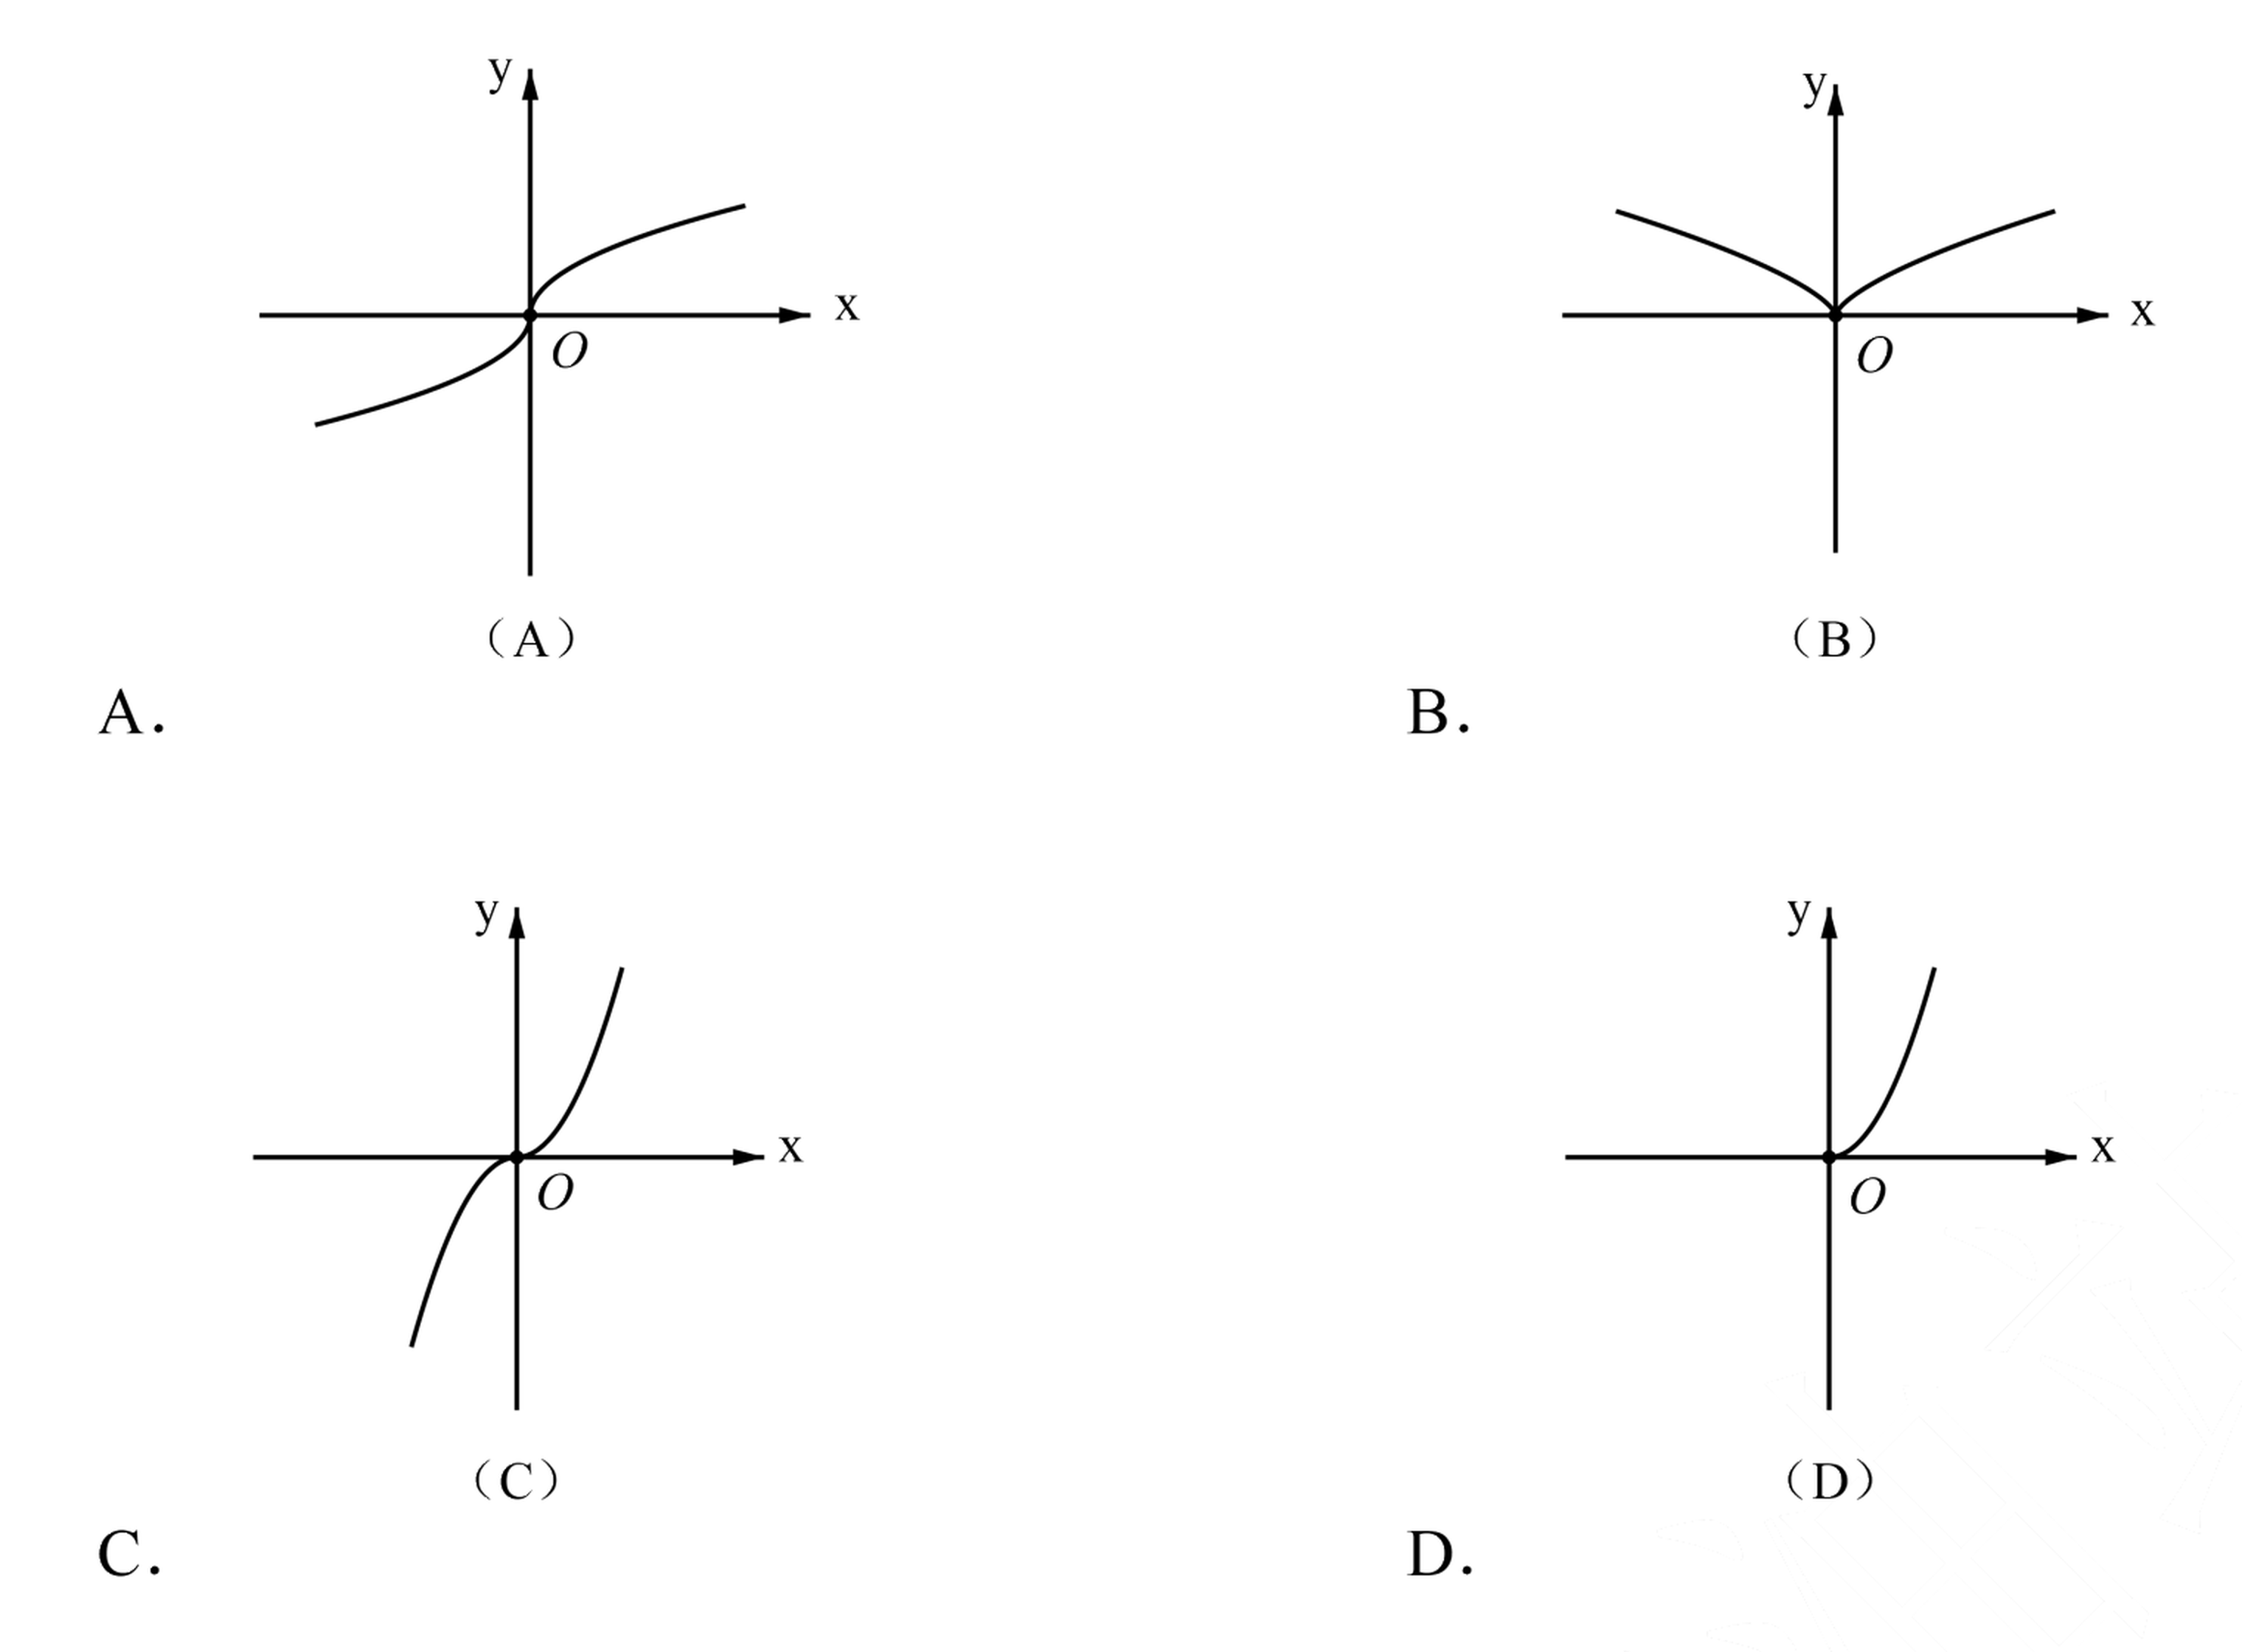
\includegraphics[width=0.80\textwidth]{figures/gao140_q14.png}
\end{center}

\ifanswer
\solbegin
\step{$f(x)=x^{\frac23}=\sqrt[3]{x^2}$ 是偶函数，且恒大于等于 $0$，故选 $B$.}
\solend
\fi

\item 设 $p$：关于 $x$ 的不等式 $x^2+ax+1>0$ 对 $x\in\R$ 恒成立，$q$：对数函数 $y=\log_{4-3a}x$ 在 $(0,+\infty)$ 上单调递减，那么 $p$ 是 $q$ 的\mbox{（\quad）}

\keepwithprev
A. 充分不必要条件\qquad B. 充要条件

C. 必要不充分条件\qquad D. 既不充分也不必要条件

\ifanswer
\solbegin
\step{$p\Leftrightarrow a^2-4<0\Leftrightarrow -2<a<2$. $q\Leftrightarrow 0<4-3a<1\Leftrightarrow 1<a<\dfrac43$.}
\step{由 $\left(1,\dfrac43\right)\subset(-2,2)$ 得 $q\Rightarrow p$；而 $a=0$ 时 $p$ 真、$q$ 假，}% 子集符号原卷印单线 $\subset$，照录
\step{故 $p$ 是 $q$ 的必要不充分条件，故选 $C$.}
\solend
\fi

\item “非空集合 $M$ 的元素都是集合 $P$ 的元素” 是假命题，现有下列命题：

(1) $M$ 的元素都不是 $P$ 的元素；(2) $M$ 中有不属于 $P$ 元素；% 原卷"不属于 P 元素"脱"的"字，照录

(3) $M$ 中有 $P$ 的元素；(4) $M$ 的元素不都是 $P$ 的元素，

其中真命题的个数是\mbox{（\quad）}

\keepwithprev
A. 1\qquad B. 2\qquad C. 3\qquad D. 4

\ifanswer
\solbegin
\step{由于 “非空集合 $M$ 的元素都是集合 $P$ 的元素” 是假命题，}
\step{得 “非空集合 $M$ 的元素至少有一个元素不属于集合 $P$” 是真命题.}
\step{则 (1) 不正确；(2) 正确；(3) $M$ 中不一定有 $P$ 的元素，例如 $M=\{a\}$，}
\step{则 $a\notin P$；(4) 正确.}
\step{综上，真命题只有 (2)(4). 故选 $B$.}
\solend
\fi

\end{enumerate}

\bigsec{三、解答题}

\begin{enumerate}
\setcounter{enumi}{16}

\item 设全集为 $\R$，集合 $A=\left\{x\mid\dfrac{2x}{x-1}\leqslant1\right\}$.

(1) 用区间表示集合 $A$；

(2) 若集合 $B=\{x\mid\lvert x+2\rvert+\lvert x-1\rvert=3\}$，求 $A\cup B$.

\ifanswer
\solbegin
\step{(1) 由 $\dfrac{2x}{x-1}\leqslant1\Leftrightarrow\dfrac{x+1}{x-1}\leqslant0$，故 $A=[-1,1)$，则 $\overline{A}=(-\infty,-1)\cup[1,+\infty)$；}
\step{(2) 由 $B=\{x\mid\lvert x+2\rvert+\lvert x-1\rvert=3\}=[-2,1]$，}
\step{结合上一问有 $A=[-1,1)$，所以 $A\cup B=B=[-2,1]$.}
\solend
\fi

\item (1) 已知指数函数 $y=a^x(a>0$ 且 $a\neq1)$ 在区间 $[-1,1]$ 上的最大值与最小值之和等于 $\dfrac52$，求实数 $a$ 的值.

(2) 已知幂函数 $y=x^{m^2+7m+10}(m\in\Z)$ 的图像关于 $y$ 轴对称，且在 $(0,+\infty)$ 上严格减. 若 $(a-1)^{m^2+7m+10}\geqslant(1+2a)^{m^2+7m+10}$. 求实数 $a$ 的取值范围.

\ifanswer
\solbegin
\step{(1) 指数函数 $y=a^x$ 在区间 $[-1,1]$ 上单调，所以 $a^1+a^{-1}=\dfrac52$，}
\step{所以 $a=2$ 或 $a=\dfrac12$；}
\step{(2) 由题意得 $m^2+7m+10<0$，所以 $-5<m<-2$，又因为 $m\in\Z$，}
\step{所以 $m=-4$ 或 $m=-3$，}
\step{当 $m=-4$ 时，$y=x^{m^2+7m+10}=x^{-2}$，为偶函数，}
\step{当 $m=-3$ 时，$y=x^{m^2+7m+10}=x^{-2}$，为偶函数，}
\step{所以 $m^2+7m+10=-2$，所以 $(a-1)^{-2}\geqslant(1+2a)^{-2}$，}
\step{所以 $\lvert a-1\rvert\leqslant\lvert 1+2a\rvert$，所以 $a\leqslant-2$ 或 $a\geqslant0$，所以 $a\in(-\infty,-2]\cup[0,+\infty)$.}
\solend
\fi

\item 设函数 $f(x)=ax^2+(1-a)x+a-2$ （$a\in\R$）.

(1) 若关于 $x$ 的不等式 $f(x)\leqslant0$ 的解集为 $\left[0,\dfrac12\right]$，求实数 $a$ 的值；

(2) 若 $a\geqslant0$，解关于 $x$ 的不等式：$f(x)<a-1$.

\ifanswer
\solbegin
\step{(1) 由解集得 $a>0$，且 $0$ 是方程 $f(x)=0$ 的根，故 $f(0)=a-2=0$，}
\step{得 $a=2$.}
\step{此时 $f(x)=2x^2-x=x(2x-1)$，$f(x)\leqslant0$ 的解集确为 $\left[0,\dfrac12\right]$.}
\step{(2) $f(x)<a-1\Leftrightarrow ax^2+(1-a)x-1<0\Leftrightarrow(x-1)(ax+1)<0$，}
\step{当 $a=0$ 时，$x-1<0$，解集为 $(-\infty,1)$.}
\step{当 $a>0$ 时，$-\dfrac1a<1$，解集为 $\left(-\dfrac1a,1\right)$.}
\solend
\fi

\item 为了保护环境，某单位采用新工艺，把二氧化碳转化为一种可利用的化工产品，已知该单位每月处理量最多不超过 $300$ 吨. 当月处理量为 $x$ 吨时，月处理成本为 $x^2-200x+40000(0<x\leqslant300)$ 元，且每处理一吨二氧化碳得到可利用的化工产品价值为 $300$ 元.

(1) 若要保证该单位每月不亏损，则每月处理量应控制在什么范围？

(2) 该单位每月处理量为多少吨时，才能使每吨的平均处理成本最低，最低为多少元？

\ifanswer
\solbegin
\step{(1) 由题意得 $S=300x-(x^2-200x+40000)$}
\step{$=-x^2+500x-40000(0<x\leqslant300)$，}
\step{令 $S\geqslant0$，即 $-x^2+500x-40000\geqslant0$，解得 $100\leqslant x\leqslant400$，}
\step{又 $0<x\leqslant300$，所以 $100\leqslant x\leqslant300$，}
\step{故要保证该单位每月不亏损，则每月处理量应控制在 $[100,300]$ 范围内；}
\step{(2) 每吨的平均出来成本为 $\dfrac yx=x+\dfrac{40000}x-200\geqslant2\sqrt{x\cdot\dfrac{40000}x}-200=200$，}% 原卷"平均出来成本"与题干"平均处理成本"措辞不一，照录
\step{当且仅当 $x=\dfrac{40000}x$，即 $x=200$ 时取等号，}
\step{所以该单位每月处理量为 $200$ 吨时，}
\step{才能使每吨的平均处理成本最低且最低为 $200$ 元.}
\solend
\fi

\item 已知函数 $y=f(x),x\in D$，若对于定义域 $D$ 内任意实数 $x,y$，不等式 $f(x)+f(y)\geqslant f(xy)$ 都成立，则称函数 $y=f(x)$ 是 $QB$ 函数，

(1) 判断函数 $f(x)=x+1$ 是否是 $QB$ 函数，并说明理由；

(2) 若函数 $g(x)=\ln(ax),x>0$ 是 $QB$ 函数，求实数 $a$ 的取值范围；

(3) 已知函数 $h(x)=a^x(a\in\R\text{ 且 }a>0)$，证明：“函数 $y=h(x)$ 是 $QB$ 函数” 的充要条件是 “ $a\in\{1\}$ ”.

\ifanswer
\solbegin
\step{(1) 不是，理由如下：因为 $f(x)=x+1$，}
\step{所以 $f(x)+f(y)\geqslant f(xy)\Leftrightarrow x+y\geqslant xy-1\Leftrightarrow(x-1)(y-1)\leqslant2$，}
\step{显然不恒成立，故不是 $QB$ 函数；}
\step{(2) 因为函数 $g(x)=\ln(ax),x>0$，则 $a>0$，}
\step{若函数 $g(x)$ 是 $QB$ 函数，则 $g(x)+g(y)\geqslant g(xy)$，}
\step{即 $\ln(ax)+\ln(ay)\geqslant\ln(axy)$，则 $\ln(a^2xy)\geqslant\ln(axy)$，得 $a^2xy\geqslant axy$，}
\step{且 $x>0,y>0$，得 $a^2\geqslant a$，解得 $a\geqslant1$ 或 $a\leqslant0$（舍去），}
\step{所以实数 $a$ 的取值范围为 $[1,+\infty)$.}
\step{(3) 若函数 $h(x)=a^x$ 是 $QB$ 函数，}
\step{当 $a>1$ 时，令 $x=y=\log_a\dfrac12$，则 $h(x)+h(y)=a^x+a^y=\dfrac12+\dfrac12=1$，}
\step{且 $h(xy)=a^{xy}=(a^x)^y=\left(\dfrac12\right)^{\log_a\frac12}=2^{\log_a2}$，}
\step{因为 $\log_a2>0$，所以 $h(xy)=2^{\log_a2}>1$，不满足 $h(x)+h(y)\geqslant h(xy)$，}
\step{不合题意；}
\step{当 $a=1$ 时，$h(x)+h(y)=a^x+a^y=1+1=2$，且 $h(xy)=a^{xy}=1$，}
\step{满足 $h(x)+h(y)\geqslant h(xy)$，符合题意；}
\step{当 $0<a<1$ 时，令 $x=\log_a2,y=2$，则 $h(x)+h(y)=a^x+a^y=2+a^2$，}
\step{且 $h(xy)=a^{xy}=(a^x)^y=2^2=4$，}
\step{因为 $0<a<1$，所以 $0<a^2<1$，得 $2<2+a^2<3$，}
\step{不满足 $h(x)+h(y)\geqslant h(xy)$，不合题意；}
\step{综上所述，$a\in\{1\}$，即充分性成立；}% 原卷"充分性/必要性"两标签与所证方向互换，照录
\step{若 $a\in\{1\}$，则 $h(x)+h(y)=a^x+a^y=1+1=2$，且 $h(xy)=a^{xy}=1$，}
\step{得 $h(x)+h(y)\geqslant h(xy)$，所以函数 $h(x)=a^x$ 是 $QB$ 函数，即必要性成立；}% 原卷"充分性/必要性"两标签与所证方向互换，照录
\step{综上所述，“函数 $y=h(x)$ 是 $QB$ 函数” 的充要条件是 “ $a\in\{1\}$ ”.}
\solend
\fi

\end{enumerate}

\end{document}
"
%
% ① 原始材料：微信公众号"魔都数学加油站"文章，连载"27学年高一140"，原文标题
% "27学年高一140——2026-2027年上海市甘泉外国语高一上期中"；
% 原文链接：https://mp.weixin.qq.com/s/eflgf2Ktk1LyT9x-k-ltLw。
% 正文为 9 张 PNG 页（01、02、03、05、06、07、08 为 4762x6735；04、09 为 2560x3620，
% 同一篇各页分辨率不同，逐页按各自分辨率裁图核对），题目下印有【答案】或【解析】，为讲评版。
% 题目、解析均据原图转录；卷面粉红色水印"魔都数学加油站"及公众号页脚未录入。
% 全卷 1 幅插图：第 14 题四幅坐标函数图象选项（04 页），取原卷截图去粉色水印、去色、
% LANCZOS 放大 2 倍，四幅选项按原卷 2x2 排布（含（A）（B）（C）（D）图注与 A./B./C./D.
% 选项字母）合并裁为一张；图前按惯例加 \needvspace 守卫。
%
% 卷首标题：原卷印作"2026-2027 年甘泉外国语高一上期中"（公众号标题中的"上海市"
% 卷面标题行没有，本稿照卷面），年份区间按全稿惯例排 en dash；原卷未印副标题，
% 本卷为期中卷、跨集合与常用逻辑用语／不等式／函数三章，按题目内容标为
% "集合与常用逻辑用语、不等式、函数"（与 125／126／128／129／131／132／133 同期中卷口径相同）：
% 集合与逻辑见 Q5、Q13、Q15、Q16、Q17，不等式见 Q3、Q10、Q11、Q19、Q20，
% 函数（指数／对数／幂函数及其图象、同构与 QB 函数）见 Q4、Q6、Q7、Q8、Q12、Q14、Q18、Q21。
%
% 题号体例：本卷共 19 题——一、填空题 3—12（10 题）、二、选择题 13—16（4 题）、
% 三、解答题 17—21（5 题）。三节分别 \setcounter{enumi}{2}／{12}／{16}。
% 原卷从第 3 题起、无第 1、2 题，本稿保留原题号。
%
% ② 与原卷的排版差异：
%   ① 原文从第 3 题起，本稿保留原题号；
%   ② 原卷每题下直接印【答案】或【解析】，本稿按全稿惯例置于答案版；第 5 题只印
%      【答案】、无【解析】，提 \ans{}；第 13、14、15、16 题答案均在【解析】末句
%      "故选 …"，题干括号内留空、不另提 \ans{}；其余各题印【解析】、无独立答案段；
%      全卷无"答案印在题干括号内且无解析"的一型；
%   ③ 原卷未印副标题，本稿按"知识模块"口径补出；
%   ④ 原卷填空横线按全稿惯例排为 \blankline[4.4em]；选择题括号排 \mbox{（\quad）}、
%      每个选项段前按惯例加 \keepwithprev（四幅图选项那一枚放在 \begin{center} 之前）；
%      解答题不留作答区、不加 \anspace（原卷为讲评版，与 129／131／132／133／136 同）；
%   ⑤ 原卷数集混排：斜体 $R$（Q9、Q12、Q15 等）与黑体／黑板粗体 $R$（Q15、Q17、
%      Q19、Q21）、粗体 $Z$（Q18），按全稿惯例统一改 \R／\Z；空集记号 \varnothing；
%      绝对值排 \lvert…\rvert，集合描述竖线排 \mid；不等号按全稿惯例排 \leqslant／\geqslant；
%      补集照原卷上划线排 \overline{A}；
%   ⑥ 子题标号 (1)(2)(3)(4) 原卷印半角括号，照录（与 131／132／133／134／136 同口径）；
%      括注原卷全角／半角混用，逐处照录：Q8"（结果用 a,b 表示）"、Q19"（a∈R）"、
%      Q21 (2)"（舍去）"印全角，Q18"$a^x(a>0$ 且 $a\neq1)$"、Q20"$40000(0<x\leqslant300)$"、
%      Q21 (3)"($a\in\R$ 且 $a>0$)"及 (0,+∞)、2(a>0) 等数学式内括注印半角；
%   ⑦ 数学式内半角逗号照录（如 Q8"$\lg2=a,10^b=3$"、Q11"$-2,3,4,\cdots,2027$"、
%      Q12"$x_1,x_2$"、Q19"$f(x)=ax^2+(1-a)x+a-2$"、Q21"$x>0,y>0$"）；
%      原卷行末西文句点照录（Q20 题干"300 吨. 当月处理量为 x 吨时"），行中全角逗号照录；
%   ⑧ 一幅插图：第 14 题四幅坐标函数图象选项合并裁为一张 \includegraphics
%      （题前 \needvspace{9cm}）。Q14 是"二、选择题"节内带大图块的第二题
%      （Q13 为节首题但无图），另在 \bigsec{二、选择题} 之前加 \needvspace{11cm}
%      连节标题一起量——守卫必须放在 \bigsec 之前，放标题之后会让"二、选择题"
%      孤立在页末（B 类，照 高一26／40／59／136 成例）；三版切页审计均"合计异常：无"；
%   ⑨ 跨页续印按题合并：Q9 题干在 01 页、解析续至 02 页；Q11 题干与解析前 3 行在 02 页、
%      后 2 行在 03 页；Q14 题干在 03 页末、四幅图与【解析】在 04 页；Q16 题干四条命题
%      在 04 页、选项与【解析】在 05 页；Q18 解析 (1) 首行在 05 页、其余 7 行在 06 页；
%      Q20 题干在 06 页末、"300 元."与两小问及【解析】在 07 页；Q21 解析跨 07—09 页
%      （末 3 行在 09 页）；本稿按题连排，不丢行；
%   ⑩ 题干中的中文弯引号按原卷照录，注释内一律 ASCII 引号；原卷"图像／图象"
%      两种写法混用，逐处照录（Q7、Q18 作"图像"，Q14 作"图象"）；
%   ⑪ 原卷无红色加粗标签（【解析】【答案】均黑色印刷），故本卷未用 \stepm。
%
% 判别式字形：全卷仅第 9 题【解析】"经验证得"cases 块出现两处判别式
%   "$\Delta=p^2-4q>0$"与"$\Delta'=q^2-4p>0$"，原卷两处均印等腰、偏高的
%   三角 $\Delta$（带撇的为 $\Delta'$），逐处放大核对并照录 \Delta、\Delta'；
%   全卷未出现扁等边三角 \triangle。
%
% 子集符号：第 15 题【解析】"由 (1,4/3)⊂(-2,2) 得 q⇒p"一处原卷印单线 $\subset$
%   （不带下划线），逐处放大核对、照录 \subset；全卷未出现带下划线的 \subseteq。
%
% 原卷存疑照录（均照录未改，正文对应处另有 % 注）：
%   第 16 题 (2) 命题"$M$ 中有不属于 $P$ 元素"中"不属于 $P$ 元素"脱"的"字，照录；
%   第 20 题题干 (2) 作"每吨的平均处理成本"、而【解析】(2) 作"每吨的平均出来成本"，
%      "出来"疑为"处理"之误，两处措辞照录不统一；
%   第 21 题 (3)【解析】"综上所述，$a\in\{1\}$，即充分性成立"与"即必要性成立"
%      两处标签与所证方向互换（按充要条件的通常口径），照录。
%
% 行数复核：一条 \step = 原卷解析的一个印刷行，cases 块作一个印刷行计。逐题数 \step
%   条数，合计 92 条（Q3：2；Q4：1；Q5：0；Q6：2；Q7：1；Q8：1；Q9：7；Q10：5；
%   Q11：5；Q12：4；Q13：6；Q14：1；Q15：3；Q16：5；Q17：3；Q18：8；Q19：6；
%   Q20：9；Q21：23），与原卷印刷行逐题相等。第 5 题只印【答案】、提 \ans{}，
%   不计入 \step 账；第 13、14、15、16 题答案在解析末句"故选 …"，括号内留空、
%   不另提 \ans{}；答案版【答案】/【解析】标记数 = 19（1 个 \ans + 18 个 \solbegin）
%   = 全卷题数。
%
\documentclass[a4paper,11pt]{article}
\usepackage{common}

\begin{document}

\examtitlest[3]{2026--2027 年甘泉外国语高一上期中}{集合与常用逻辑用语、不等式、函数}

\bigsec{一、填空题}

\begin{enumerate}
\setcounter{enumi}{2}

\item 不等式 $x^2-2x-3<0$ 的解集为\blankline[4.4em].

\ifanswer
\solbegin
\step{方程 $x^2-2x-3=0$ 的实数根是 $x_1=-1$，$x_2=3$；}
\step{所以不等式 $x^2-2x-3<0$ 的解集为 $\{x\mid -1<x<3\}$.}
\solend
\fi

\item 根式 $\sqrt{x\sqrt{x}}(x>0)$ 的指数幂形式为\blankline[4.4em].

\ifanswer
\solbegin
\step{$\sqrt{x\sqrt{x}}=\sqrt{x\cdot x^{\frac12}}=\sqrt{x^{\frac32}}=x^{\frac34}$.}
\solend
\fi

\item 陈述句 “ $x>1$ 或 $y>1$ ” 的否定形式是\blankline[4.4em].

\ifanswer
\ans{$x\leqslant1$ 且 $y\leqslant1$}
\fi

\item 若 $x<0$ 时，指数函数 $y=(a-1)^x$ 的值总大于 $1$，则实数 $a$ 的取值范围是\blankline[4.4em].

\ifanswer
\solbegin
\step{由题意得 $(a-1)^x>1$ 在 $(-\infty,0)$ 上恒成立，则 $0<a-1<1$，解得 $1<a<2$.}
\step{故实数 $a$ 的取值范围是 $(1,2)$.}
\solend
\fi

\item 若 $f(x)=\log_a(x-1)$，对任意 $a>0$ 且 $a\neq1$，函数 $y=f(x)$ 的图像必过定点\blankline[4.4em].

\ifanswer
\solbegin
\step{令 $x-1=1$，即 $x=2$，此时 $f(2)=0$，即函数图像过定点 $(2,0)$.}
\solend
\fi

\item 已知 $\lg 2=a,10^b=3$，则 $\log_6 2=$\blankline[4.4em]（结果用 $a,b$ 表示）.

\ifanswer
\solbegin
\step{由 $10^b=3$，得 $b=\lg 3$，则 $\log_6 2=\dfrac{\lg 2}{\lg 6}=\dfrac{\lg 2}{\lg 2+\lg 3}=\dfrac{a}{a+b}$.}
\solend
\fi

\item 已知 $p$、$q\in\R$，$x_1$、$x_2$ 是关于 $x$ 的方程 $x^2+px+q=0$ 的两实根，$x_1+1$、$x_2+1$ 是关于 $x$ 的方程 $x^2+qx+p=0$ 的两实根，则 $pq=$\blankline[4.4em].

\ifanswer
\solbegin
\step{因为 $x_1$、$x_2$ 是关于 $x$ 的方程 $x^2+px+q=0$ 的两实根，}
\step{由韦达定理得 $x_1+x_2=-p$，$x_1\cdot x_2=q$，}
\step{因为 $x_1+1$、$x_2+1$ 是关于 $x$ 的方程 $x^2+qx+p=0$ 的两实根，}
\step{由韦达定理得 $x_1+1+x_2+1=-q$，$(x_1+1)(x_2+1)=p$，}
\step{即 $x_1+x_2=-q-2$，$x_1+x_2+x_1x_2=p-1$，又 $x_1+x_2=-p$，$x_1\cdot x_2=q$，}
\step{所以 $\begin{cases}-p=-q-2\\-p+q=p-1\end{cases}$，解得 $\begin{cases}p=-1\\q=-3\end{cases}$，经验证得 $\begin{cases}\Delta=p^2-4q>0\\\Delta'=q^2-4p>0\end{cases}$，}% 判别式原卷印高三角 $\Delta$、$\Delta'$，照录
\step{则 $pq=3$.}
\solend
\fi

\item 对于 $x\in\R$，不等式 $\lvert 3-x\rvert+\lvert 1+x\rvert\geqslant a^2-3a$ 恒成立，则实数 $a$ 的取值范围是\blankline[4.4em].

\ifanswer
\solbegin
\step{对于 $x\in\R$，不等式 $\lvert 3-x\rvert+\lvert 1+x\rvert\geqslant a^2-3a$ 恒成立，}
\step{即 $\lvert 3-x\rvert+\lvert 1+x\rvert$ 的最小值大于或等于 $a^2-3a$，}
\step{$\lvert 3-x\rvert+\lvert 1+x\rvert$ 表示数轴上的 $x$ 对应点到 $3$ 和 $-1$ 对应点的距离之和，}
\step{它的最小值为 $4$，故 $4\geqslant a^2-3a$，即 $a^2-3a-4\leqslant0$，解得 $-1\leqslant a\leqslant4$，}
\step{故实数 $a$ 的取值范围是 $[-1,4]$.}
\solend
\fi

\item 已知同时满足不等式 $x^2-x-2>0$ 和 $2x^2+(5+2a)x+5a<0$ 的 $x$ 的整数值只有 $2026$ 个，则实数 $a$ 的取值范围是\blankline[4.4em].

\ifanswer
\solbegin
\step{整数 $x$ 须满足 $x\leqslant-2$ 或 $x\geqslant3$，且 $(2x+5)(x+a)<0$.}
\step{当 $a<\dfrac52$ 时，需使整数解恰为 $-2,3,4,\cdots,2027$，即 $2027<-a\leqslant2028$.}
\step{当 $a>\dfrac52$ 时，需使整数解恰为 $-2028,-2027,\cdots,-3$，即 $2028<a\leqslant2029$；}
\step{$a=\dfrac52$ 时无解.}
\step{故 $a\in[-2028,-2027)\cup(2028,2029]$.}
\solend
\fi

\item 同构式通俗讲是结构相同的表达式，如：$f(x)=x+e^x$，$f(\ln x)=\ln x+e^{\ln x}=\ln x+x$，称 $x+e^x$ 与 $\ln x+x$ 为同构式. 已知实数 $x_1,x_2$ 满足 $e^{x_1}+x_1=8,\ln\sqrt[5]{5x_2+3}+x_2=1$，则 $x_1+5x_2=$\blankline[4.4em].

\ifanswer
\solbegin
\step{函数 $f(x)=x+e^x$ 在 $\R$ 上严格增，且 $f(x_1)=x_1+e^{x_1}=8$，}
\step{由 $\ln\sqrt[5]{5x_2+3}+x_2=1$，得 $\ln(5x_2+3)+5x_2=5$，则 $\ln(5x_2+3)+5x_2+3=8$，}
\step{即 $f(\ln(5x_2+3))=8$，因此 $f(\ln(5x_2+3))=8=f(x_1)$，则 $x_1=\ln(5x_2+3)$，}
\step{所以 $x_1+5x_2=\ln(5x_2+3)+5x_2=5$.}
\solend
\fi

\end{enumerate}

% 第 14 题四幅图是"二、选择题"节内的大图块；守卫须放在 \bigsec 之前连节标题一起量，
% 否则"二、选择题"会孤立在页末（B 类，照 高一26／40／59／136 成例）
\needvspace{11cm}
\bigsec{二、选择题}

\begin{enumerate}
\setcounter{enumi}{12}

\item 设 $a$、$b$ 为实数，则 “ $a>b>0$ ” 的一个充分非必要条件是\mbox{（\quad）}

\keepwithprev
A. $\sqrt{a-1}>\sqrt{b-1}$\qquad B. $a^2>b^2$

C. $\dfrac1b>\dfrac1a$\qquad D. $a-b>b-a$

\ifanswer
\solbegin
\step{由 $\sqrt{a-1}>\sqrt{b-1}$ 得 $a>b\geqslant1$，故 $a>b>0$，反之不成立，满足题意；}
\step{由 $a^2>b^2$，则 $\lvert a\rvert>\lvert b\rvert$，推不出 $a>b>0$，反向可推出，不满足；}
\step{由 $\dfrac1b>\dfrac1a$，则 $a>b>0$ 或 $b>0>a$ 或 $0>a>b$，推不出 $a>b>0$，}
\step{反向可推出，不满足；}
\step{由 $a-b>b-a$，则 $a>b$，推不出 $a>b>0$，反向可推出，不满足；}
\step{故选 $A$.}
\solend
\fi

% 第 14 题四幅坐标函数图象选项是一整块，守卫放在 \item 之前
\needvspace{9cm}
\item 幂函数 $f(x)=x^{\frac23}$ 的图象大致为\mbox{（\quad）}

\keepwithprev
\begin{center}
% 四幅坐标函数图象选项取原卷 04 页截图去粉色水印、去色，按原卷 2x2 排布合并为一张
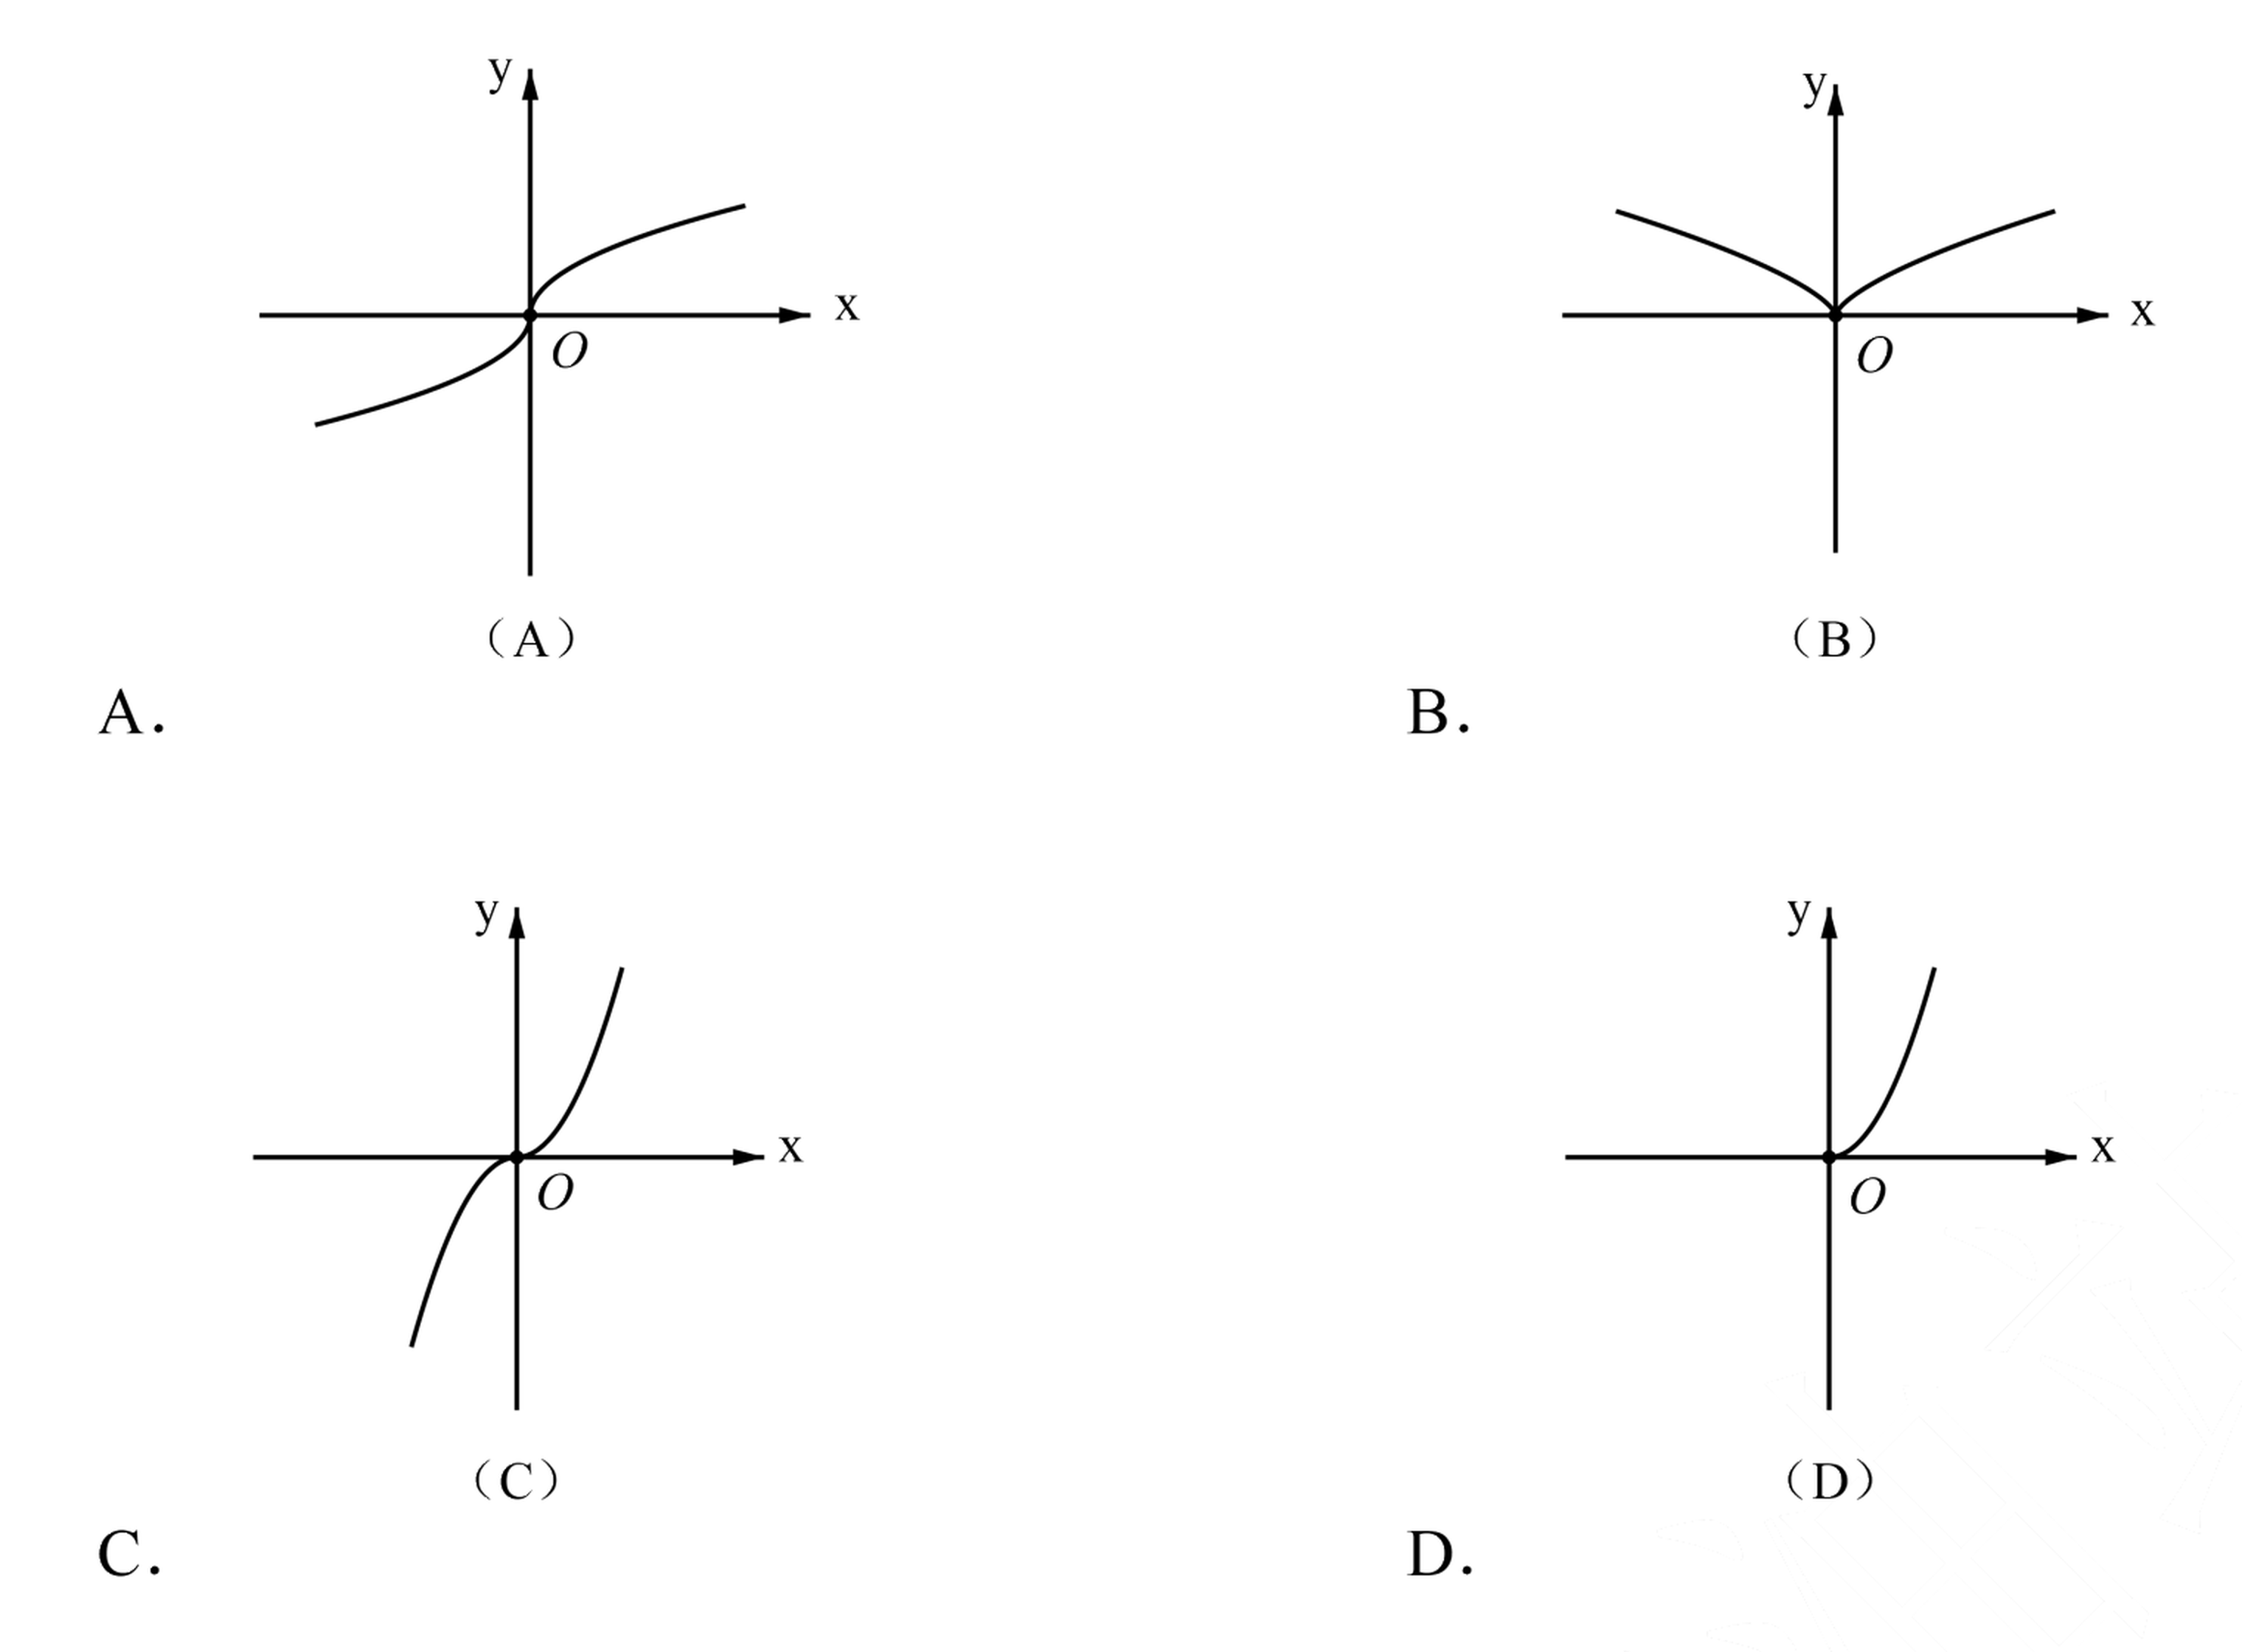
\includegraphics[width=0.80\textwidth]{figures/gao140_q14.png}
\end{center}

\ifanswer
\solbegin
\step{$f(x)=x^{\frac23}=\sqrt[3]{x^2}$ 是偶函数，且恒大于等于 $0$，故选 $B$.}
\solend
\fi

\item 设 $p$：关于 $x$ 的不等式 $x^2+ax+1>0$ 对 $x\in\R$ 恒成立，$q$：对数函数 $y=\log_{4-3a}x$ 在 $(0,+\infty)$ 上单调递减，那么 $p$ 是 $q$ 的\mbox{（\quad）}

\keepwithprev
A. 充分不必要条件\qquad B. 充要条件

C. 必要不充分条件\qquad D. 既不充分也不必要条件

\ifanswer
\solbegin
\step{$p\Leftrightarrow a^2-4<0\Leftrightarrow -2<a<2$. $q\Leftrightarrow 0<4-3a<1\Leftrightarrow 1<a<\dfrac43$.}
\step{由 $\left(1,\dfrac43\right)\subset(-2,2)$ 得 $q\Rightarrow p$；而 $a=0$ 时 $p$ 真、$q$ 假，}% 子集符号原卷印单线 $\subset$，照录
\step{故 $p$ 是 $q$ 的必要不充分条件，故选 $C$.}
\solend
\fi

\item “非空集合 $M$ 的元素都是集合 $P$ 的元素” 是假命题，现有下列命题：

(1) $M$ 的元素都不是 $P$ 的元素；(2) $M$ 中有不属于 $P$ 元素；% 原卷"不属于 P 元素"脱"的"字，照录

(3) $M$ 中有 $P$ 的元素；(4) $M$ 的元素不都是 $P$ 的元素，

其中真命题的个数是\mbox{（\quad）}

\keepwithprev
A. 1\qquad B. 2\qquad C. 3\qquad D. 4

\ifanswer
\solbegin
\step{由于 “非空集合 $M$ 的元素都是集合 $P$ 的元素” 是假命题，}
\step{得 “非空集合 $M$ 的元素至少有一个元素不属于集合 $P$” 是真命题.}
\step{则 (1) 不正确；(2) 正确；(3) $M$ 中不一定有 $P$ 的元素，例如 $M=\{a\}$，}
\step{则 $a\notin P$；(4) 正确.}
\step{综上，真命题只有 (2)(4). 故选 $B$.}
\solend
\fi

\end{enumerate}

\bigsec{三、解答题}

\begin{enumerate}
\setcounter{enumi}{16}

\item 设全集为 $\R$，集合 $A=\left\{x\mid\dfrac{2x}{x-1}\leqslant1\right\}$.

(1) 用区间表示集合 $A$；

(2) 若集合 $B=\{x\mid\lvert x+2\rvert+\lvert x-1\rvert=3\}$，求 $A\cup B$.

\ifanswer
\solbegin
\step{(1) 由 $\dfrac{2x}{x-1}\leqslant1\Leftrightarrow\dfrac{x+1}{x-1}\leqslant0$，故 $A=[-1,1)$，则 $\overline{A}=(-\infty,-1)\cup[1,+\infty)$；}
\step{(2) 由 $B=\{x\mid\lvert x+2\rvert+\lvert x-1\rvert=3\}=[-2,1]$，}
\step{结合上一问有 $A=[-1,1)$，所以 $A\cup B=B=[-2,1]$.}
\solend
\fi

\item (1) 已知指数函数 $y=a^x(a>0$ 且 $a\neq1)$ 在区间 $[-1,1]$ 上的最大值与最小值之和等于 $\dfrac52$，求实数 $a$ 的值.

(2) 已知幂函数 $y=x^{m^2+7m+10}(m\in\Z)$ 的图像关于 $y$ 轴对称，且在 $(0,+\infty)$ 上严格减. 若 $(a-1)^{m^2+7m+10}\geqslant(1+2a)^{m^2+7m+10}$. 求实数 $a$ 的取值范围.

\ifanswer
\solbegin
\step{(1) 指数函数 $y=a^x$ 在区间 $[-1,1]$ 上单调，所以 $a^1+a^{-1}=\dfrac52$，}
\step{所以 $a=2$ 或 $a=\dfrac12$；}
\step{(2) 由题意得 $m^2+7m+10<0$，所以 $-5<m<-2$，又因为 $m\in\Z$，}
\step{所以 $m=-4$ 或 $m=-3$，}
\step{当 $m=-4$ 时，$y=x^{m^2+7m+10}=x^{-2}$，为偶函数，}
\step{当 $m=-3$ 时，$y=x^{m^2+7m+10}=x^{-2}$，为偶函数，}
\step{所以 $m^2+7m+10=-2$，所以 $(a-1)^{-2}\geqslant(1+2a)^{-2}$，}
\step{所以 $\lvert a-1\rvert\leqslant\lvert 1+2a\rvert$，所以 $a\leqslant-2$ 或 $a\geqslant0$，所以 $a\in(-\infty,-2]\cup[0,+\infty)$.}
\solend
\fi

\item 设函数 $f(x)=ax^2+(1-a)x+a-2$ （$a\in\R$）.

(1) 若关于 $x$ 的不等式 $f(x)\leqslant0$ 的解集为 $\left[0,\dfrac12\right]$，求实数 $a$ 的值；

(2) 若 $a\geqslant0$，解关于 $x$ 的不等式：$f(x)<a-1$.

\ifanswer
\solbegin
\step{(1) 由解集得 $a>0$，且 $0$ 是方程 $f(x)=0$ 的根，故 $f(0)=a-2=0$，}
\step{得 $a=2$.}
\step{此时 $f(x)=2x^2-x=x(2x-1)$，$f(x)\leqslant0$ 的解集确为 $\left[0,\dfrac12\right]$.}
\step{(2) $f(x)<a-1\Leftrightarrow ax^2+(1-a)x-1<0\Leftrightarrow(x-1)(ax+1)<0$，}
\step{当 $a=0$ 时，$x-1<0$，解集为 $(-\infty,1)$.}
\step{当 $a>0$ 时，$-\dfrac1a<1$，解集为 $\left(-\dfrac1a,1\right)$.}
\solend
\fi

\item 为了保护环境，某单位采用新工艺，把二氧化碳转化为一种可利用的化工产品，已知该单位每月处理量最多不超过 $300$ 吨. 当月处理量为 $x$ 吨时，月处理成本为 $x^2-200x+40000(0<x\leqslant300)$ 元，且每处理一吨二氧化碳得到可利用的化工产品价值为 $300$ 元.

(1) 若要保证该单位每月不亏损，则每月处理量应控制在什么范围？

(2) 该单位每月处理量为多少吨时，才能使每吨的平均处理成本最低，最低为多少元？

\ifanswer
\solbegin
\step{(1) 由题意得 $S=300x-(x^2-200x+40000)$}
\step{$=-x^2+500x-40000(0<x\leqslant300)$，}
\step{令 $S\geqslant0$，即 $-x^2+500x-40000\geqslant0$，解得 $100\leqslant x\leqslant400$，}
\step{又 $0<x\leqslant300$，所以 $100\leqslant x\leqslant300$，}
\step{故要保证该单位每月不亏损，则每月处理量应控制在 $[100,300]$ 范围内；}
\step{(2) 每吨的平均出来成本为 $\dfrac yx=x+\dfrac{40000}x-200\geqslant2\sqrt{x\cdot\dfrac{40000}x}-200=200$，}% 原卷"平均出来成本"与题干"平均处理成本"措辞不一，照录
\step{当且仅当 $x=\dfrac{40000}x$，即 $x=200$ 时取等号，}
\step{所以该单位每月处理量为 $200$ 吨时，}
\step{才能使每吨的平均处理成本最低且最低为 $200$ 元.}
\solend
\fi

\item 已知函数 $y=f(x),x\in D$，若对于定义域 $D$ 内任意实数 $x,y$，不等式 $f(x)+f(y)\geqslant f(xy)$ 都成立，则称函数 $y=f(x)$ 是 $QB$ 函数，

(1) 判断函数 $f(x)=x+1$ 是否是 $QB$ 函数，并说明理由；

(2) 若函数 $g(x)=\ln(ax),x>0$ 是 $QB$ 函数，求实数 $a$ 的取值范围；

(3) 已知函数 $h(x)=a^x(a\in\R\text{ 且 }a>0)$，证明：“函数 $y=h(x)$ 是 $QB$ 函数” 的充要条件是 “ $a\in\{1\}$ ”.

\ifanswer
\solbegin
\step{(1) 不是，理由如下：因为 $f(x)=x+1$，}
\step{所以 $f(x)+f(y)\geqslant f(xy)\Leftrightarrow x+y\geqslant xy-1\Leftrightarrow(x-1)(y-1)\leqslant2$，}
\step{显然不恒成立，故不是 $QB$ 函数；}
\step{(2) 因为函数 $g(x)=\ln(ax),x>0$，则 $a>0$，}
\step{若函数 $g(x)$ 是 $QB$ 函数，则 $g(x)+g(y)\geqslant g(xy)$，}
\step{即 $\ln(ax)+\ln(ay)\geqslant\ln(axy)$，则 $\ln(a^2xy)\geqslant\ln(axy)$，得 $a^2xy\geqslant axy$，}
\step{且 $x>0,y>0$，得 $a^2\geqslant a$，解得 $a\geqslant1$ 或 $a\leqslant0$（舍去），}
\step{所以实数 $a$ 的取值范围为 $[1,+\infty)$.}
\step{(3) 若函数 $h(x)=a^x$ 是 $QB$ 函数，}
\step{当 $a>1$ 时，令 $x=y=\log_a\dfrac12$，则 $h(x)+h(y)=a^x+a^y=\dfrac12+\dfrac12=1$，}
\step{且 $h(xy)=a^{xy}=(a^x)^y=\left(\dfrac12\right)^{\log_a\frac12}=2^{\log_a2}$，}
\step{因为 $\log_a2>0$，所以 $h(xy)=2^{\log_a2}>1$，不满足 $h(x)+h(y)\geqslant h(xy)$，}
\step{不合题意；}
\step{当 $a=1$ 时，$h(x)+h(y)=a^x+a^y=1+1=2$，且 $h(xy)=a^{xy}=1$，}
\step{满足 $h(x)+h(y)\geqslant h(xy)$，符合题意；}
\step{当 $0<a<1$ 时，令 $x=\log_a2,y=2$，则 $h(x)+h(y)=a^x+a^y=2+a^2$，}
\step{且 $h(xy)=a^{xy}=(a^x)^y=2^2=4$，}
\step{因为 $0<a<1$，所以 $0<a^2<1$，得 $2<2+a^2<3$，}
\step{不满足 $h(x)+h(y)\geqslant h(xy)$，不合题意；}
\step{综上所述，$a\in\{1\}$，即充分性成立；}% 原卷"充分性/必要性"两标签与所证方向互换，照录
\step{若 $a\in\{1\}$，则 $h(x)+h(y)=a^x+a^y=1+1=2$，且 $h(xy)=a^{xy}=1$，}
\step{得 $h(x)+h(y)\geqslant h(xy)$，所以函数 $h(x)=a^x$ 是 $QB$ 函数，即必要性成立；}% 原卷"充分性/必要性"两标签与所证方向互换，照录
\step{综上所述，“函数 $y=h(x)$ 是 $QB$ 函数” 的充要条件是 “ $a\in\{1\}$ ”.}
\solend
\fi

\end{enumerate}

\end{document}
"
%
% ① 原始材料：微信公众号"魔都数学加油站"文章，连载"27学年高一140"，原文标题
% "27学年高一140——2026-2027年上海市甘泉外国语高一上期中"；
% 原文链接：https://mp.weixin.qq.com/s/eflgf2Ktk1LyT9x-k-ltLw。
% 正文为 9 张 PNG 页（01、02、03、05、06、07、08 为 4762x6735；04、09 为 2560x3620，
% 同一篇各页分辨率不同，逐页按各自分辨率裁图核对），题目下印有【答案】或【解析】，为讲评版。
% 题目、解析均据原图转录；卷面粉红色水印"魔都数学加油站"及公众号页脚未录入。
% 全卷 1 幅插图：第 14 题四幅坐标函数图象选项（04 页），取原卷截图去粉色水印、去色、
% LANCZOS 放大 2 倍，四幅选项按原卷 2x2 排布（含（A）（B）（C）（D）图注与 A./B./C./D.
% 选项字母）合并裁为一张；图前按惯例加 \needvspace 守卫。
%
% 卷首标题：原卷印作"2026-2027 年甘泉外国语高一上期中"（公众号标题中的"上海市"
% 卷面标题行没有，本稿照卷面），年份区间按全稿惯例排 en dash；原卷未印副标题，
% 本卷为期中卷、跨集合与常用逻辑用语／不等式／函数三章，按题目内容标为
% "集合与常用逻辑用语、不等式、函数"（与 125／126／128／129／131／132／133 同期中卷口径相同）：
% 集合与逻辑见 Q5、Q13、Q15、Q16、Q17，不等式见 Q3、Q10、Q11、Q19、Q20，
% 函数（指数／对数／幂函数及其图象、同构与 QB 函数）见 Q4、Q6、Q7、Q8、Q12、Q14、Q18、Q21。
%
% 题号体例：本卷共 19 题——一、填空题 3—12（10 题）、二、选择题 13—16（4 题）、
% 三、解答题 17—21（5 题）。三节分别 \setcounter{enumi}{2}／{12}／{16}。
% 原卷从第 3 题起、无第 1、2 题，本稿保留原题号。
%
% ② 与原卷的排版差异：
%   ① 原文从第 3 题起，本稿保留原题号；
%   ② 原卷每题下直接印【答案】或【解析】，本稿按全稿惯例置于答案版；第 5 题只印
%      【答案】、无【解析】，提 \ans{}；第 13、14、15、16 题答案均在【解析】末句
%      "故选 …"，题干括号内留空、不另提 \ans{}；其余各题印【解析】、无独立答案段；
%      全卷无"答案印在题干括号内且无解析"的一型；
%   ③ 原卷未印副标题，本稿按"知识模块"口径补出；
%   ④ 原卷填空横线按全稿惯例排为 \blankline[4.4em]；选择题括号排 \mbox{（\quad）}、
%      每个选项段前按惯例加 \keepwithprev（四幅图选项那一枚放在 \begin{center} 之前）；
%      解答题不留作答区、不加 \anspace（原卷为讲评版，与 129／131／132／133／136 同）；
%   ⑤ 原卷数集混排：斜体 $R$（Q9、Q12、Q15 等）与黑体／黑板粗体 $R$（Q15、Q17、
%      Q19、Q21）、粗体 $Z$（Q18），按全稿惯例统一改 \R／\Z；空集记号 \varnothing；
%      绝对值排 \lvert…\rvert，集合描述竖线排 \mid；不等号按全稿惯例排 \leqslant／\geqslant；
%      补集照原卷上划线排 \overline{A}；
%   ⑥ 子题标号 (1)(2)(3)(4) 原卷印半角括号，照录（与 131／132／133／134／136 同口径）；
%      括注原卷全角／半角混用，逐处照录：Q8"（结果用 a,b 表示）"、Q19"（a∈R）"、
%      Q21 (2)"（舍去）"印全角，Q18"$a^x(a>0$ 且 $a\neq1)$"、Q20"$40000(0<x\leqslant300)$"、
%      Q21 (3)"($a\in\R$ 且 $a>0$)"及 (0,+∞)、2(a>0) 等数学式内括注印半角；
%   ⑦ 数学式内半角逗号照录（如 Q8"$\lg2=a,10^b=3$"、Q11"$-2,3,4,\cdots,2027$"、
%      Q12"$x_1,x_2$"、Q19"$f(x)=ax^2+(1-a)x+a-2$"、Q21"$x>0,y>0$"）；
%      原卷行末西文句点照录（Q20 题干"300 吨. 当月处理量为 x 吨时"），行中全角逗号照录；
%   ⑧ 一幅插图：第 14 题四幅坐标函数图象选项合并裁为一张 \includegraphics
%      （题前 \needvspace{9cm}）。Q14 是"二、选择题"节内带大图块的第二题
%      （Q13 为节首题但无图），另在 \bigsec{二、选择题} 之前加 \needvspace{11cm}
%      连节标题一起量——守卫必须放在 \bigsec 之前，放标题之后会让"二、选择题"
%      孤立在页末（B 类，照 高一26／40／59／136 成例）；三版切页审计均"合计异常：无"；
%   ⑨ 跨页续印按题合并：Q9 题干在 01 页、解析续至 02 页；Q11 题干与解析前 3 行在 02 页、
%      后 2 行在 03 页；Q14 题干在 03 页末、四幅图与【解析】在 04 页；Q16 题干四条命题
%      在 04 页、选项与【解析】在 05 页；Q18 解析 (1) 首行在 05 页、其余 7 行在 06 页；
%      Q20 题干在 06 页末、"300 元."与两小问及【解析】在 07 页；Q21 解析跨 07—09 页
%      （末 3 行在 09 页）；本稿按题连排，不丢行；
%   ⑩ 题干中的中文弯引号按原卷照录，注释内一律 ASCII 引号；原卷"图像／图象"
%      两种写法混用，逐处照录（Q7、Q18 作"图像"，Q14 作"图象"）；
%   ⑪ 原卷无红色加粗标签（【解析】【答案】均黑色印刷），故本卷未用 \stepm。
%
% 判别式字形：全卷仅第 9 题【解析】"经验证得"cases 块出现两处判别式
%   "$\Delta=p^2-4q>0$"与"$\Delta'=q^2-4p>0$"，原卷两处均印等腰、偏高的
%   三角 $\Delta$（带撇的为 $\Delta'$），逐处放大核对并照录 \Delta、\Delta'；
%   全卷未出现扁等边三角 \triangle。
%
% 子集符号：第 15 题【解析】"由 (1,4/3)⊂(-2,2) 得 q⇒p"一处原卷印单线 $\subset$
%   （不带下划线），逐处放大核对、照录 \subset；全卷未出现带下划线的 \subseteq。
%
% 原卷存疑照录（均照录未改，正文对应处另有 % 注）：
%   第 16 题 (2) 命题"$M$ 中有不属于 $P$ 元素"中"不属于 $P$ 元素"脱"的"字，照录；
%   第 20 题题干 (2) 作"每吨的平均处理成本"、而【解析】(2) 作"每吨的平均出来成本"，
%      "出来"疑为"处理"之误，两处措辞照录不统一；
%   第 21 题 (3)【解析】"综上所述，$a\in\{1\}$，即充分性成立"与"即必要性成立"
%      两处标签与所证方向互换（按充要条件的通常口径），照录。
%
% 行数复核：一条 \step = 原卷解析的一个印刷行，cases 块作一个印刷行计。逐题数 \step
%   条数，合计 92 条（Q3：2；Q4：1；Q5：0；Q6：2；Q7：1；Q8：1；Q9：7；Q10：5；
%   Q11：5；Q12：4；Q13：6；Q14：1；Q15：3；Q16：5；Q17：3；Q18：8；Q19：6；
%   Q20：9；Q21：23），与原卷印刷行逐题相等。第 5 题只印【答案】、提 \ans{}，
%   不计入 \step 账；第 13、14、15、16 题答案在解析末句"故选 …"，括号内留空、
%   不另提 \ans{}；答案版【答案】/【解析】标记数 = 19（1 个 \ans + 18 个 \solbegin）
%   = 全卷题数。
%
\documentclass[a4paper,11pt]{article}
\usepackage{common}

\begin{document}

\examtitlest[3]{2026--2027 年甘泉外国语高一上期中}{集合与常用逻辑用语、不等式、函数}

\bigsec{一、填空题}

\begin{enumerate}
\setcounter{enumi}{2}

\item 不等式 $x^2-2x-3<0$ 的解集为\blankline[4.4em].

\ifanswer
\solbegin
\step{方程 $x^2-2x-3=0$ 的实数根是 $x_1=-1$，$x_2=3$；}
\step{所以不等式 $x^2-2x-3<0$ 的解集为 $\{x\mid -1<x<3\}$.}
\solend
\fi

\item 根式 $\sqrt{x\sqrt{x}}(x>0)$ 的指数幂形式为\blankline[4.4em].

\ifanswer
\solbegin
\step{$\sqrt{x\sqrt{x}}=\sqrt{x\cdot x^{\frac12}}=\sqrt{x^{\frac32}}=x^{\frac34}$.}
\solend
\fi

\item 陈述句 “ $x>1$ 或 $y>1$ ” 的否定形式是\blankline[4.4em].

\ifanswer
\ans{$x\leqslant1$ 且 $y\leqslant1$}
\fi

\item 若 $x<0$ 时，指数函数 $y=(a-1)^x$ 的值总大于 $1$，则实数 $a$ 的取值范围是\blankline[4.4em].

\ifanswer
\solbegin
\step{由题意得 $(a-1)^x>1$ 在 $(-\infty,0)$ 上恒成立，则 $0<a-1<1$，解得 $1<a<2$.}
\step{故实数 $a$ 的取值范围是 $(1,2)$.}
\solend
\fi

\item 若 $f(x)=\log_a(x-1)$，对任意 $a>0$ 且 $a\neq1$，函数 $y=f(x)$ 的图像必过定点\blankline[4.4em].

\ifanswer
\solbegin
\step{令 $x-1=1$，即 $x=2$，此时 $f(2)=0$，即函数图像过定点 $(2,0)$.}
\solend
\fi

\item 已知 $\lg 2=a,10^b=3$，则 $\log_6 2=$\blankline[4.4em]（结果用 $a,b$ 表示）.

\ifanswer
\solbegin
\step{由 $10^b=3$，得 $b=\lg 3$，则 $\log_6 2=\dfrac{\lg 2}{\lg 6}=\dfrac{\lg 2}{\lg 2+\lg 3}=\dfrac{a}{a+b}$.}
\solend
\fi

\item 已知 $p$、$q\in\R$，$x_1$、$x_2$ 是关于 $x$ 的方程 $x^2+px+q=0$ 的两实根，$x_1+1$、$x_2+1$ 是关于 $x$ 的方程 $x^2+qx+p=0$ 的两实根，则 $pq=$\blankline[4.4em].

\ifanswer
\solbegin
\step{因为 $x_1$、$x_2$ 是关于 $x$ 的方程 $x^2+px+q=0$ 的两实根，}
\step{由韦达定理得 $x_1+x_2=-p$，$x_1\cdot x_2=q$，}
\step{因为 $x_1+1$、$x_2+1$ 是关于 $x$ 的方程 $x^2+qx+p=0$ 的两实根，}
\step{由韦达定理得 $x_1+1+x_2+1=-q$，$(x_1+1)(x_2+1)=p$，}
\step{即 $x_1+x_2=-q-2$，$x_1+x_2+x_1x_2=p-1$，又 $x_1+x_2=-p$，$x_1\cdot x_2=q$，}
\step{所以 $\begin{cases}-p=-q-2\\-p+q=p-1\end{cases}$，解得 $\begin{cases}p=-1\\q=-3\end{cases}$，经验证得 $\begin{cases}\Delta=p^2-4q>0\\\Delta'=q^2-4p>0\end{cases}$，}% 判别式原卷印高三角 $\Delta$、$\Delta'$，照录
\step{则 $pq=3$.}
\solend
\fi

\item 对于 $x\in\R$，不等式 $\lvert 3-x\rvert+\lvert 1+x\rvert\geqslant a^2-3a$ 恒成立，则实数 $a$ 的取值范围是\blankline[4.4em].

\ifanswer
\solbegin
\step{对于 $x\in\R$，不等式 $\lvert 3-x\rvert+\lvert 1+x\rvert\geqslant a^2-3a$ 恒成立，}
\step{即 $\lvert 3-x\rvert+\lvert 1+x\rvert$ 的最小值大于或等于 $a^2-3a$，}
\step{$\lvert 3-x\rvert+\lvert 1+x\rvert$ 表示数轴上的 $x$ 对应点到 $3$ 和 $-1$ 对应点的距离之和，}
\step{它的最小值为 $4$，故 $4\geqslant a^2-3a$，即 $a^2-3a-4\leqslant0$，解得 $-1\leqslant a\leqslant4$，}
\step{故实数 $a$ 的取值范围是 $[-1,4]$.}
\solend
\fi

\item 已知同时满足不等式 $x^2-x-2>0$ 和 $2x^2+(5+2a)x+5a<0$ 的 $x$ 的整数值只有 $2026$ 个，则实数 $a$ 的取值范围是\blankline[4.4em].

\ifanswer
\solbegin
\step{整数 $x$ 须满足 $x\leqslant-2$ 或 $x\geqslant3$，且 $(2x+5)(x+a)<0$.}
\step{当 $a<\dfrac52$ 时，需使整数解恰为 $-2,3,4,\cdots,2027$，即 $2027<-a\leqslant2028$.}
\step{当 $a>\dfrac52$ 时，需使整数解恰为 $-2028,-2027,\cdots,-3$，即 $2028<a\leqslant2029$；}
\step{$a=\dfrac52$ 时无解.}
\step{故 $a\in[-2028,-2027)\cup(2028,2029]$.}
\solend
\fi

\item 同构式通俗讲是结构相同的表达式，如：$f(x)=x+e^x$，$f(\ln x)=\ln x+e^{\ln x}=\ln x+x$，称 $x+e^x$ 与 $\ln x+x$ 为同构式. 已知实数 $x_1,x_2$ 满足 $e^{x_1}+x_1=8,\ln\sqrt[5]{5x_2+3}+x_2=1$，则 $x_1+5x_2=$\blankline[4.4em].

\ifanswer
\solbegin
\step{函数 $f(x)=x+e^x$ 在 $\R$ 上严格增，且 $f(x_1)=x_1+e^{x_1}=8$，}
\step{由 $\ln\sqrt[5]{5x_2+3}+x_2=1$，得 $\ln(5x_2+3)+5x_2=5$，则 $\ln(5x_2+3)+5x_2+3=8$，}
\step{即 $f(\ln(5x_2+3))=8$，因此 $f(\ln(5x_2+3))=8=f(x_1)$，则 $x_1=\ln(5x_2+3)$，}
\step{所以 $x_1+5x_2=\ln(5x_2+3)+5x_2=5$.}
\solend
\fi

\end{enumerate}

% 第 14 题四幅图是"二、选择题"节内的大图块；守卫须放在 \bigsec 之前连节标题一起量，
% 否则"二、选择题"会孤立在页末（B 类，照 高一26／40／59／136 成例）
\needvspace{11cm}
\bigsec{二、选择题}

\begin{enumerate}
\setcounter{enumi}{12}

\item 设 $a$、$b$ 为实数，则 “ $a>b>0$ ” 的一个充分非必要条件是\mbox{（\quad）}

\keepwithprev
A. $\sqrt{a-1}>\sqrt{b-1}$\qquad B. $a^2>b^2$

C. $\dfrac1b>\dfrac1a$\qquad D. $a-b>b-a$

\ifanswer
\solbegin
\step{由 $\sqrt{a-1}>\sqrt{b-1}$ 得 $a>b\geqslant1$，故 $a>b>0$，反之不成立，满足题意；}
\step{由 $a^2>b^2$，则 $\lvert a\rvert>\lvert b\rvert$，推不出 $a>b>0$，反向可推出，不满足；}
\step{由 $\dfrac1b>\dfrac1a$，则 $a>b>0$ 或 $b>0>a$ 或 $0>a>b$，推不出 $a>b>0$，}
\step{反向可推出，不满足；}
\step{由 $a-b>b-a$，则 $a>b$，推不出 $a>b>0$，反向可推出，不满足；}
\step{故选 $A$.}
\solend
\fi

% 第 14 题四幅坐标函数图象选项是一整块，守卫放在 \item 之前
\needvspace{9cm}
\item 幂函数 $f(x)=x^{\frac23}$ 的图象大致为\mbox{（\quad）}

\keepwithprev
\begin{center}
% 四幅坐标函数图象选项取原卷 04 页截图去粉色水印、去色，按原卷 2x2 排布合并为一张
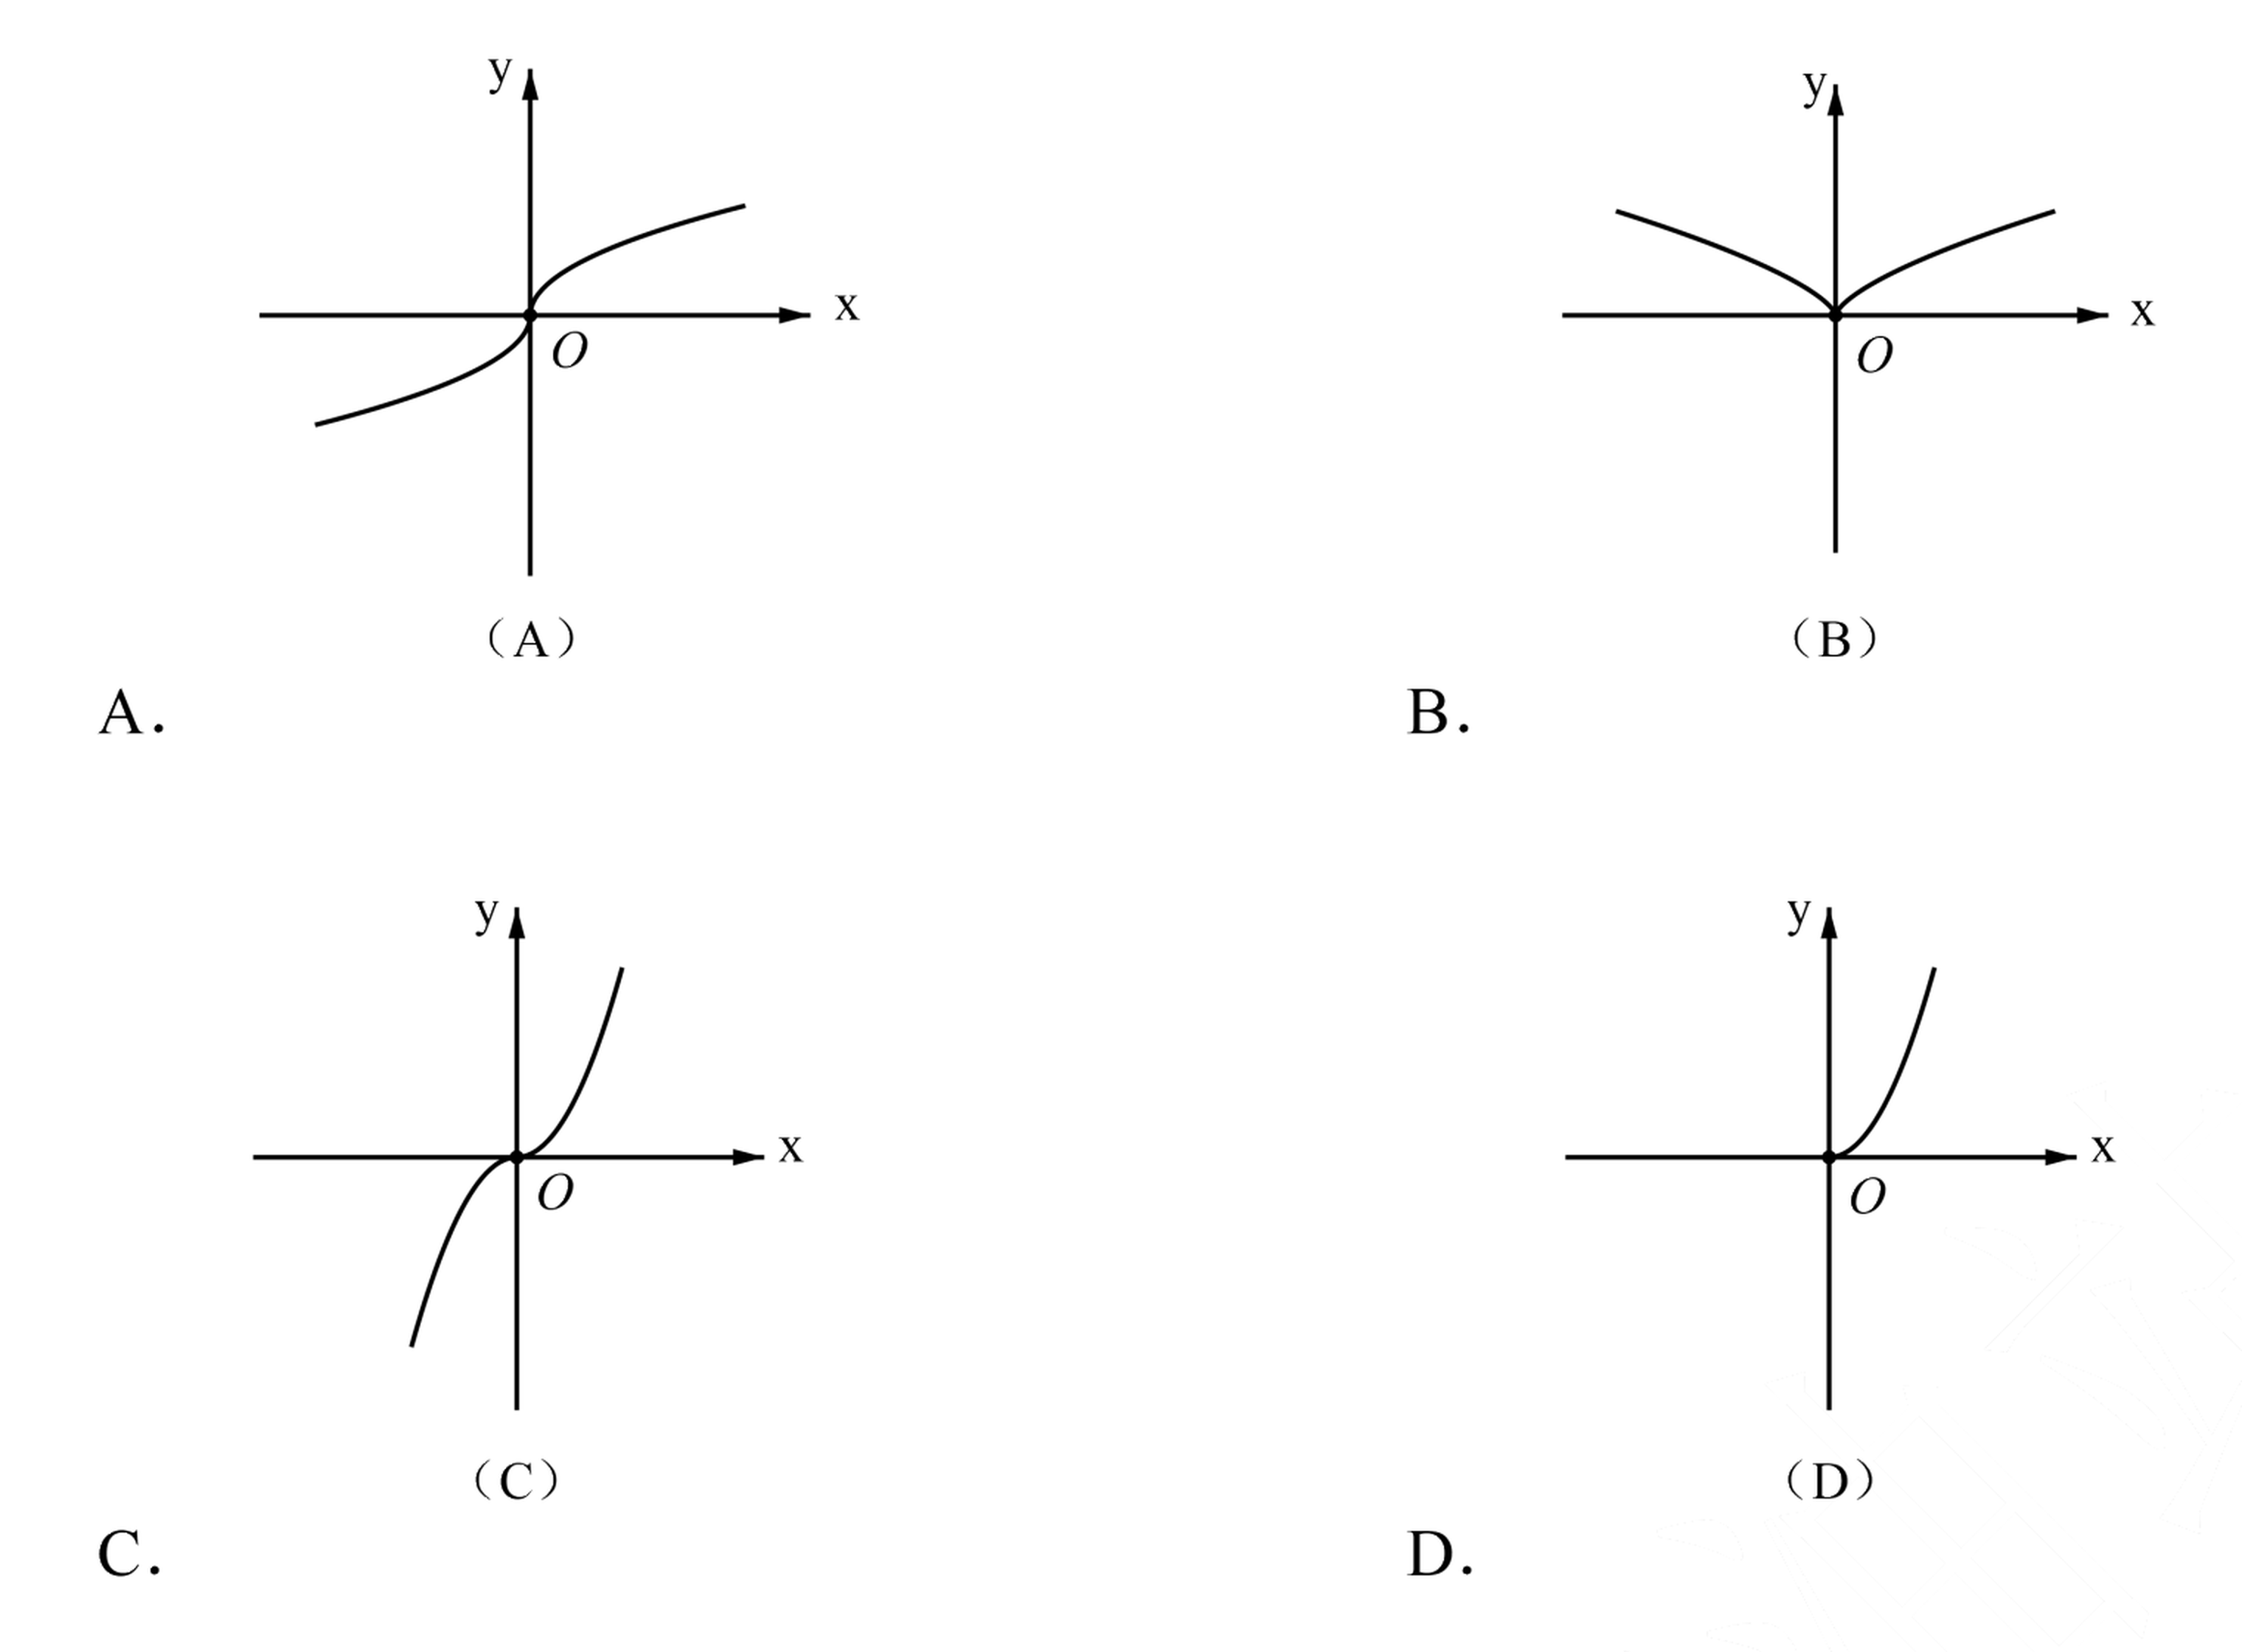
\includegraphics[width=0.80\textwidth]{figures/gao140_q14.png}
\end{center}

\ifanswer
\solbegin
\step{$f(x)=x^{\frac23}=\sqrt[3]{x^2}$ 是偶函数，且恒大于等于 $0$，故选 $B$.}
\solend
\fi

\item 设 $p$：关于 $x$ 的不等式 $x^2+ax+1>0$ 对 $x\in\R$ 恒成立，$q$：对数函数 $y=\log_{4-3a}x$ 在 $(0,+\infty)$ 上单调递减，那么 $p$ 是 $q$ 的\mbox{（\quad）}

\keepwithprev
A. 充分不必要条件\qquad B. 充要条件

C. 必要不充分条件\qquad D. 既不充分也不必要条件

\ifanswer
\solbegin
\step{$p\Leftrightarrow a^2-4<0\Leftrightarrow -2<a<2$. $q\Leftrightarrow 0<4-3a<1\Leftrightarrow 1<a<\dfrac43$.}
\step{由 $\left(1,\dfrac43\right)\subset(-2,2)$ 得 $q\Rightarrow p$；而 $a=0$ 时 $p$ 真、$q$ 假，}% 子集符号原卷印单线 $\subset$，照录
\step{故 $p$ 是 $q$ 的必要不充分条件，故选 $C$.}
\solend
\fi

\item “非空集合 $M$ 的元素都是集合 $P$ 的元素” 是假命题，现有下列命题：

(1) $M$ 的元素都不是 $P$ 的元素；(2) $M$ 中有不属于 $P$ 元素；% 原卷"不属于 P 元素"脱"的"字，照录

(3) $M$ 中有 $P$ 的元素；(4) $M$ 的元素不都是 $P$ 的元素，

其中真命题的个数是\mbox{（\quad）}

\keepwithprev
A. 1\qquad B. 2\qquad C. 3\qquad D. 4

\ifanswer
\solbegin
\step{由于 “非空集合 $M$ 的元素都是集合 $P$ 的元素” 是假命题，}
\step{得 “非空集合 $M$ 的元素至少有一个元素不属于集合 $P$” 是真命题.}
\step{则 (1) 不正确；(2) 正确；(3) $M$ 中不一定有 $P$ 的元素，例如 $M=\{a\}$，}
\step{则 $a\notin P$；(4) 正确.}
\step{综上，真命题只有 (2)(4). 故选 $B$.}
\solend
\fi

\end{enumerate}

\bigsec{三、解答题}

\begin{enumerate}
\setcounter{enumi}{16}

\item 设全集为 $\R$，集合 $A=\left\{x\mid\dfrac{2x}{x-1}\leqslant1\right\}$.

(1) 用区间表示集合 $A$；

(2) 若集合 $B=\{x\mid\lvert x+2\rvert+\lvert x-1\rvert=3\}$，求 $A\cup B$.

\ifanswer
\solbegin
\step{(1) 由 $\dfrac{2x}{x-1}\leqslant1\Leftrightarrow\dfrac{x+1}{x-1}\leqslant0$，故 $A=[-1,1)$，则 $\overline{A}=(-\infty,-1)\cup[1,+\infty)$；}
\step{(2) 由 $B=\{x\mid\lvert x+2\rvert+\lvert x-1\rvert=3\}=[-2,1]$，}
\step{结合上一问有 $A=[-1,1)$，所以 $A\cup B=B=[-2,1]$.}
\solend
\fi

\item (1) 已知指数函数 $y=a^x(a>0$ 且 $a\neq1)$ 在区间 $[-1,1]$ 上的最大值与最小值之和等于 $\dfrac52$，求实数 $a$ 的值.

(2) 已知幂函数 $y=x^{m^2+7m+10}(m\in\Z)$ 的图像关于 $y$ 轴对称，且在 $(0,+\infty)$ 上严格减. 若 $(a-1)^{m^2+7m+10}\geqslant(1+2a)^{m^2+7m+10}$. 求实数 $a$ 的取值范围.

\ifanswer
\solbegin
\step{(1) 指数函数 $y=a^x$ 在区间 $[-1,1]$ 上单调，所以 $a^1+a^{-1}=\dfrac52$，}
\step{所以 $a=2$ 或 $a=\dfrac12$；}
\step{(2) 由题意得 $m^2+7m+10<0$，所以 $-5<m<-2$，又因为 $m\in\Z$，}
\step{所以 $m=-4$ 或 $m=-3$，}
\step{当 $m=-4$ 时，$y=x^{m^2+7m+10}=x^{-2}$，为偶函数，}
\step{当 $m=-3$ 时，$y=x^{m^2+7m+10}=x^{-2}$，为偶函数，}
\step{所以 $m^2+7m+10=-2$，所以 $(a-1)^{-2}\geqslant(1+2a)^{-2}$，}
\step{所以 $\lvert a-1\rvert\leqslant\lvert 1+2a\rvert$，所以 $a\leqslant-2$ 或 $a\geqslant0$，所以 $a\in(-\infty,-2]\cup[0,+\infty)$.}
\solend
\fi

\item 设函数 $f(x)=ax^2+(1-a)x+a-2$ （$a\in\R$）.

(1) 若关于 $x$ 的不等式 $f(x)\leqslant0$ 的解集为 $\left[0,\dfrac12\right]$，求实数 $a$ 的值；

(2) 若 $a\geqslant0$，解关于 $x$ 的不等式：$f(x)<a-1$.

\ifanswer
\solbegin
\step{(1) 由解集得 $a>0$，且 $0$ 是方程 $f(x)=0$ 的根，故 $f(0)=a-2=0$，}
\step{得 $a=2$.}
\step{此时 $f(x)=2x^2-x=x(2x-1)$，$f(x)\leqslant0$ 的解集确为 $\left[0,\dfrac12\right]$.}
\step{(2) $f(x)<a-1\Leftrightarrow ax^2+(1-a)x-1<0\Leftrightarrow(x-1)(ax+1)<0$，}
\step{当 $a=0$ 时，$x-1<0$，解集为 $(-\infty,1)$.}
\step{当 $a>0$ 时，$-\dfrac1a<1$，解集为 $\left(-\dfrac1a,1\right)$.}
\solend
\fi

\item 为了保护环境，某单位采用新工艺，把二氧化碳转化为一种可利用的化工产品，已知该单位每月处理量最多不超过 $300$ 吨. 当月处理量为 $x$ 吨时，月处理成本为 $x^2-200x+40000(0<x\leqslant300)$ 元，且每处理一吨二氧化碳得到可利用的化工产品价值为 $300$ 元.

(1) 若要保证该单位每月不亏损，则每月处理量应控制在什么范围？

(2) 该单位每月处理量为多少吨时，才能使每吨的平均处理成本最低，最低为多少元？

\ifanswer
\solbegin
\step{(1) 由题意得 $S=300x-(x^2-200x+40000)$}
\step{$=-x^2+500x-40000(0<x\leqslant300)$，}
\step{令 $S\geqslant0$，即 $-x^2+500x-40000\geqslant0$，解得 $100\leqslant x\leqslant400$，}
\step{又 $0<x\leqslant300$，所以 $100\leqslant x\leqslant300$，}
\step{故要保证该单位每月不亏损，则每月处理量应控制在 $[100,300]$ 范围内；}
\step{(2) 每吨的平均出来成本为 $\dfrac yx=x+\dfrac{40000}x-200\geqslant2\sqrt{x\cdot\dfrac{40000}x}-200=200$，}% 原卷"平均出来成本"与题干"平均处理成本"措辞不一，照录
\step{当且仅当 $x=\dfrac{40000}x$，即 $x=200$ 时取等号，}
\step{所以该单位每月处理量为 $200$ 吨时，}
\step{才能使每吨的平均处理成本最低且最低为 $200$ 元.}
\solend
\fi

\item 已知函数 $y=f(x),x\in D$，若对于定义域 $D$ 内任意实数 $x,y$，不等式 $f(x)+f(y)\geqslant f(xy)$ 都成立，则称函数 $y=f(x)$ 是 $QB$ 函数，

(1) 判断函数 $f(x)=x+1$ 是否是 $QB$ 函数，并说明理由；

(2) 若函数 $g(x)=\ln(ax),x>0$ 是 $QB$ 函数，求实数 $a$ 的取值范围；

(3) 已知函数 $h(x)=a^x(a\in\R\text{ 且 }a>0)$，证明：“函数 $y=h(x)$ 是 $QB$ 函数” 的充要条件是 “ $a\in\{1\}$ ”.

\ifanswer
\solbegin
\step{(1) 不是，理由如下：因为 $f(x)=x+1$，}
\step{所以 $f(x)+f(y)\geqslant f(xy)\Leftrightarrow x+y\geqslant xy-1\Leftrightarrow(x-1)(y-1)\leqslant2$，}
\step{显然不恒成立，故不是 $QB$ 函数；}
\step{(2) 因为函数 $g(x)=\ln(ax),x>0$，则 $a>0$，}
\step{若函数 $g(x)$ 是 $QB$ 函数，则 $g(x)+g(y)\geqslant g(xy)$，}
\step{即 $\ln(ax)+\ln(ay)\geqslant\ln(axy)$，则 $\ln(a^2xy)\geqslant\ln(axy)$，得 $a^2xy\geqslant axy$，}
\step{且 $x>0,y>0$，得 $a^2\geqslant a$，解得 $a\geqslant1$ 或 $a\leqslant0$（舍去），}
\step{所以实数 $a$ 的取值范围为 $[1,+\infty)$.}
\step{(3) 若函数 $h(x)=a^x$ 是 $QB$ 函数，}
\step{当 $a>1$ 时，令 $x=y=\log_a\dfrac12$，则 $h(x)+h(y)=a^x+a^y=\dfrac12+\dfrac12=1$，}
\step{且 $h(xy)=a^{xy}=(a^x)^y=\left(\dfrac12\right)^{\log_a\frac12}=2^{\log_a2}$，}
\step{因为 $\log_a2>0$，所以 $h(xy)=2^{\log_a2}>1$，不满足 $h(x)+h(y)\geqslant h(xy)$，}
\step{不合题意；}
\step{当 $a=1$ 时，$h(x)+h(y)=a^x+a^y=1+1=2$，且 $h(xy)=a^{xy}=1$，}
\step{满足 $h(x)+h(y)\geqslant h(xy)$，符合题意；}
\step{当 $0<a<1$ 时，令 $x=\log_a2,y=2$，则 $h(x)+h(y)=a^x+a^y=2+a^2$，}
\step{且 $h(xy)=a^{xy}=(a^x)^y=2^2=4$，}
\step{因为 $0<a<1$，所以 $0<a^2<1$，得 $2<2+a^2<3$，}
\step{不满足 $h(x)+h(y)\geqslant h(xy)$，不合题意；}
\step{综上所述，$a\in\{1\}$，即充分性成立；}% 原卷"充分性/必要性"两标签与所证方向互换，照录
\step{若 $a\in\{1\}$，则 $h(x)+h(y)=a^x+a^y=1+1=2$，且 $h(xy)=a^{xy}=1$，}
\step{得 $h(x)+h(y)\geqslant h(xy)$，所以函数 $h(x)=a^x$ 是 $QB$ 函数，即必要性成立；}% 原卷"充分性/必要性"两标签与所证方向互换，照录
\step{综上所述，“函数 $y=h(x)$ 是 $QB$ 函数” 的充要条件是 “ $a\in\{1\}$ ”.}
\solend
\fi

\end{enumerate}

\end{document}
